\documentclass[pdftex,12pt,a4paper]{report}

\usepackage{dbstmpl}
\usepackage{hyperref}
\usepackage{amsthm}
\usepackage{graphicx}
\usepackage{wrapfig}
\usepackage{bbold}
\usepackage{aligned-overset}
\usepackage{algpseudocode}
\usepackage{algorithm}
\usepackage{placeins}
\usepackage{amsmath}
\usepackage{mdframed}
\usepackage{xcolor}
\newmdenv[
  leftmargin = 0pt,
  innerleftmargin = 1em,
  innertopmargin = 0pt,
  innerbottommargin = 0pt,
  innerrightmargin = 0pt,
  rightmargin = 0pt,
  linewidth = 3pt,
  linecolor=lightgray,
  topline = false,
  rightline = false,
  bottomline = false
  ]{leftbar}

\graphicspath{{./images/}}
\newtheorem{definition}{Definition}[section]
\newtheorem{theorem}[definition]{Theorem}
\newtheorem{alg}{Algorithm}



\newcommand{\myvec}[1]{\ensuremath{\begin{pmatrix}#1\end{pmatrix}}}
\newcommand*{\vertbar}{\rule[-1ex]{0.5pt}{2.5ex}}
\newcommand*{\horzbar}{\rule[.5ex]{2.5ex}{0.5pt}}
\newcommand\norm[1]{\left\lVert#1\right\rVert}
\newcommand\normx[1]{\left\Vert#1\right\Vert}

\newcommand\undermat[2]{%
  \makebox[0pt][l]{$\smash{\underbrace{\phantom{%
    \begin{matrix}#2\end{matrix}}}_{\text{$#1$}}}$}#2}


\global\arbeit{Master's Thesis}

\global\titel{Order Preservation in Dimensionality Reduction:\\Structure-Based Embeddings in Real and Complex Space}
\global\bearbeiter{Anna Maria Thum}
\global\betreuer{Dr. Anna Beer}
\global\aufgabensteller{Prof. Dr. Thomas Seidl}
\global\abgabetermin{6. October 2023}
\global\ort{München}
\global\fach{Computer Science}

\begin{document}

\deckblatt

\erklaerung

\begin{abstract}
In many real-world datasets, such as time series, the inherent order of data encodes valuable information.
However, commonly used dimensionality reduction methods, like Principal Component Analysis (PCA), often cannot capture this order, potentially leading to a loss of crucial insights.
In this work, we propose a new focus for dimensionality reduction methods: order-based distance preservation.
Moreover, we introduce Principal Component Analysis for Structure-Aware Representation (PCA*) and variants of Complex Principal Components Analysis (CPCA).
These methods are designed to incorporate sequential information into the dimensionality reduction process.
By considering the inherent relationships in the data, PCA* aims to provide more meaningful and informative representations.
This has the potential to enhance data analysis, visualisation, and model building in domains where order plays a critical role.
Our experiments demonstrate promising results for order-based distance preservation with PCA* in comparison to other dimensionality reduction methods including PCA, random projection and LLE.
To evaluate the quality of order-based distance preservation of dimensionality reduction methods, we employ different measures and conduct experiments on both synthetic and real-world data.

\end{abstract}

\tableofcontents

\chapter{Introduction}

High-dimensional data poses many challenges and complexities that can impede data analysis, visualisation and interpretation.
Among these challenges is the curse of dimensionality.
It describes how the data becomes sparser while the dimensionality of the data space increases, which in turn affects distance measures.
In addition to the curse of dimensionality, there are other geometric property phenomena.
Consider the volume of the unit sphere, for instance.
While the volume increases steadily from dimension one to five, it then subsequently decreases and eventually approximates zero as the dimensionality of the unit sphere reaches higher dimensions \cite{dimensionality-curse}.
Therefore reducing dimensions is an important part of data analysis.

Since there are many challenges with high-dimensional data, there are numerous dimensionality reduction methods offering effective ways to distil valuable insights.
For example, it is common to categorise dimensionality reduction techniques into local or global structure-preserving methods.
Dimensionality reduction techniques with a high degree of local structure preservation maintain the local distances and relationships between neighbouring data points.
Essentially they aim to map nearby points to nearby points in the lower-dimensional space \cite{global-vs-local-nonlinear-dim-reduction}.
Some of these techniques are Locally Linear Embedding (LLE) \cite{LLE}, t-Distributed Stochastic Neighbour Embedding (t-SNE) \cite{t-SNE} and Uniform Manifold Approximation and Projection (UMAP) \cite{umap-implementation}.
On the other hand, global structure-preserving methods aim to keep the overall relationships and trends in the data.
Principal Component Analysis (PCA) emphasises dominant patterns of variability within a population, which can capture the overall patterns and trends across the dataset.
In summary, PCA aims to capture the maximum amount of variance in the data by finding the directions of maximum variation through the principal components \cite{PCA-global-structure-preserving}.

In the above-mentioned dimensionality reduction methods the primary focus is on capturing the spatial structure of the data.
However, when dealing with ordered data, which refers to data where the arrangement or sequence of data points holds significance, these methods disregard this aspect.
Ordered data implies that the data points are organised in a specific sequence, and the relationships between adjacent points carry valuable information.
For example, time series data are ordered, as they consist of observations collected over successive time intervals, and these observations have inherent temporal dependencies \cite{dropp}.
These dependencies require specialised analysis techniques to capture trends, patterns and seasonality accurately \cite{dropp} \cite{PCA-joliffe}.
Therefore, in addition to preserving local and global structures, we introduce another essential property: order-based distance preservation for dimensionality reduction methods designed specifically for ordered data.
This property aims to ensure that the meaningful order and relationships between data points are maintained during the dimensionality reduction process.
Similarly to local structure preservation which focuses on preserving the distances of the $k$-nearest neighbours, we want to preserve the distances to the predecessor and successor of each data point in the known order.
For example, the order-preserving property ensures that in sequentially ordered data like time series the temporal relationships are accurately maintained in the lower-dimensional space.
This can aid in understanding patterns, trends and changes over time, leading to more interpretable and actionable results.

We introduce the PCA variant Principal Component Analysis for Structure-Aware Representation (PCA*) which allows us to incorporate sequential order information into the dimensionality reduction process.
By considering the vectors between successive data points in sequential data, PCA* captures the inherent relationships and dependencies within the dataset.
This approach provides therefore a deterministic way to preserve order-based distances while reducing dimensions.

Furthermore, we compare our method with PCA as well as other unsupervised dimensionality reduction methods, like LLE, t-SNE and UMAP.
Like PCA our proposed method is simple to implement and has roughly the same computational runtime as PCA.

This work is structured as follows:
in Chapter~\ref{related-work} we give an overview of the PCA algorithm.
We also explore other global and local structure-preserving dimensionality reduction methods.
Chapter~\ref{dim_red on ordered data} introduces the concept of ordered data emphasising the importance of preserving various structures, particularly order-based distance preservation.
Chapter~\ref{experiments} presents the practical aspect, including the datasets, quality measures and implementation details.
We conduct experiments on synthetic and real-world data with PCA* and the variants of CPCA.
Chapter~\ref{future-work} outlines potential future research directions in the field of order-based distance preservation and PCA*.
To conclude this work, we summarise the key findings in the last Chapter~\ref{conclusion}.


\chapter{Related Work} \label{related-work}
As the volume of collected data continues to expand, driven by ongoing improvements in technology and the complexity of real-world problems, dimensionality reduction has become a fundamental part the modern research \cite{dimensionality-curse}.
Therefore, there is a growing demand for dimensionality reduction methods with different functionalities.
To answer these needs there are diverse dimensionality reduction methods, each tailored to specific data characteristics and analytical goals.
In the following sections, we explore various dimensionality reduction methods, from global or local structure-preserving to dimensionality reduction techniques for ordered data.

\section{Global Structure Preserving Dimensionality Reduction Methods}
Global structure-preserving dimensionality reduction methods offer a profound means to retain essential information from high-dimensional data while retaining the inherent relationships and patterns within the data.
We start by examining Principal Component Analysis (PCA) and linear discriminant analysis (LDA).
Since PCA* is based on PCA, we delve deeper into the theory behind PCA. 
For other dimensionality reduction methods, we provide a brief description of their core principles.

\subsection{Principal Component Analysis} \label{PCA}

Principal Component Analysis (PCA) is one of the most often used dimensionality reduction methods due to its simplicity and non-parametricity \cite{PCA-joliffe}.
It aims to capture the most essential information within a high-dimensional dataset by transforming the data into a new lower-dimensional space with its principal components.
Principal components are the orthogonal directions in the data space accounting for the maximum variance and thus the transformation results in a new set of axes or dimensions that capture the most significant variations.
This makes PCA a powerful method for dimensionality reduction \cite{PCA-tutorial} \cite{PCA-joliffe}.
In this section, we explore how PCA works and where its strengths and weaknesses lie.

As mentioned earlier, PCA is a widely used technique in data analysis and has been defined in various contexts.
In this work, we establish our definition based on the work of \cite{PCA-optimisation}:

\begin{definition}[Principal Component Analysis] 
    Let $X$ be data in $\R ^{n \times d}$ with each row representing a $d$-dimensional data point $x_i$ with $i \in \{1, \dots, n\}$.
    PCA now aims to identify a set of $k$ orthonormal unit vectors $\mathcal{V} = [\nu_1, \dots, \nu_k]$, where each column $\nu_i$ represents a principal component capturing the directions of maximum variance in the data space and $k \leq d$.
    The goal is to maximise the variance of the data projected onto these vectors.
    Therefore, PCA can be written as an optimisation problem:
    \begin{align*}
        \max_{\mathcal{V}} \operatorname{tr}(\mathcal{V} ^T X^T X \mathcal{V}) 
    \end{align*}
    such that
    \begin{align*}
        \mathcal{V}^T \mathcal{V} = \mathbb{1}_{k \times k},
    \end{align*}
    where $ \operatorname{tr}$ denotes the trace operation, $\mathbb{1}_{k \times k}$ is the $k \times k $ unit matrix, and $X^T$ denotes the transposed matrix.
\end{definition}

In simpler terms, PCA aims to maximise the variance of the transformed data values.
The diagonal entries of the covariance matrix of the original data matrix represent these variances.
Transforming the data results in the transformed covariance matrix $\mathcal{V} ^T X^T X \mathcal{V}$ for the transformed data shown in the definition above.
By maximising the trace of this matrix, we effectively maximise the variance within the transformed data.

When using PCA we are following assumptions \cite{PCA-tutorial}:
\begin{itemize}
    \item Linearity: PCA operates on linear combinations of features and therefore, does not capture non-linear relationships or patterns in the data effectively.
    \item The larger the variance the more important: PCA uses variance as a measure of spread and by maximising this, PCA ensures to capture as much information as possible about the data's spread and variability
    \item Independence: PCA uses the covariance matrix to find the principal components, but this technique assumes certain statistical properties, including independence of the variables \cite{PCA-joliffe}.
\end{itemize}

There are multiple ways to compute PCA.
One option is using the Singular Value Decomposition (SVD) of the data matrix.
SVD is used in linear algebra to decompose a matrix into three separate matrices, which provide insights into the structure and properties of the original matrix.

For SVD, a commonly employed mathematical technique, we define it based on \cite{PCA-joliffe}:
\begin{definition}[Singular Value Decomposition]\label{SVD}
    Suppose matrix $X$ of dimension $ n \times d$ is given.
    The singular value decomposition of $X$ is as defined follows:
    \begin{align*}
        X = U \Sigma V^T,
    \end{align*}
    where
    \begin{itemize}
        \item $U$ is an $n \times d$ orthonormal matrix which is often referred to as the left singular vectors,
        \item $V$ is an $n \times d$ orthonormal matrix. It commonly is called the right singular matrix,
        \item $\Sigma$ is an $d \times d$ diagonal matrix containing the singular values of $X$. 
    \end{itemize}
\end{definition}
PCA involves finding the principal components of a dataset, which are the directions of maximum variance.
These are essentially the eigenvectors of the covariance matrix of $X$.
SVD helps to achieve this by decomposing the data such that its principal components are revealed.

First, for the dimensionality reduction of data with PCA, we prepare the data.
Let $X$ be the $n \times d$-dimensional data.
To compute the covariance matrix we need to center $X$.
Centring data is important as without it, there might be translation effects and it is not clear if the results are statistically appropriate, see \cite{relation-centered-uncentered-PCA}.
The covariance matrix is calculated as follows:
\begin{align*}
    \operatorname{Cov}(X_{\mathrm{centred}}) = \frac{1}{n} X_{\mathrm{centred}} ^T X_{\mathrm{centred}}.
\end{align*}

We show that the matrix of the left singular vectors $V$ contains the eigenvectors of the covariance matrix of X, by computing:
\begin{align*}
    \operatorname{Cov}(X_{\mathrm{centred}}) = \frac{1}{n} X_{\mathrm{centred}}^T X_{\mathrm{centred}} \overset{\text{SVD}}&{=} \frac{1}{n}(U \Sigma V^T)^T (U \Sigma V^T) = \frac{1}{n} V \Sigma^T \Sigma V^T.
\end{align*}
% Additionally, the eigenvalues of $X$ are the square root of the eigenvalues of $n \operatorname{Cov}(X_{\mathrm{centred}})$.
% If we now multiply both sides of $X_{\mathrm{centred}} = U \Sigma V^T$ with $V$ on the right, we gain $X_{\mathrm{centred}}V = U \Sigma$.
Therefore contains $\Sigma^T \Sigma$ the eigenvalues of $\operatorname{Cov}(X_{\mathrm{centred}})$ as diagonal entries and $V$ the eigenvectors, or, in the case of PCA, on $X$ the principal components.
To project the data to a lower dimensional space, we truncate $V$ to $k \leq d$ columns and multiply $X_{\mathrm{centred}}$ with the truncated matrix.
For this, we sort the eigenvalues in descending order.
The eigenvectors corresponding to the largest eigenvalues are selected, as they represent the directions of the maximum variance in the data.
We denote the truncated right singular vectors as $V_k$.

If we want to reconstruct the data from the lower-dimensional representation, we multiply the transformed data by the transpose of the principal component matrix $V_k$.
% This reconstruction step approximates the original data using the reduced principal components.
The quality of reconstruction depends on how many principal components are retained.

As PCA captures the directions in which the data varies the most, PCA effectively preserves the overall spread and dispersion of the data and preserves therefore the global structure \cite{PCA-global-structure-preserving}.

% \subsection{Independent Component Analysis}
% % Unlike PCA, independent component analysis (ICA) assumes the data not to be a linear combination of data components, it rather seeks to find statistically independent components.

% Though it can be considered an extension of PCA, independent component analysis (ICA) does not aim to find orthogonal components that capture the maximum variance in the data, rather it seeks to detect statistically independent components \cite{ICA-book}.
% ICA assumes the observed data to be linear combinations of hidden sources, and it aims to find these sources.
% It relies on the assumption that the sources themselves are statistically independent from each other.
% This means that the probability distribution of one source should not depend on the probability distribution of another source.
% By deleting or retaining some sources it can be considered a dimensionality reduction method.
% Essentially it aims to unmix the underlying sources of variation in the data.
% This is especially useful for scenarios where the observed data are mixed and overlapped, such as audio signals, images or biomedical data \cite{ICA-book}.


% Assume data $X$ consisting of $n$ linear mixtures $x_1, \dots, x_n$ of $n$ independent components:
% \begin{align*}
%     x_i = a_{i1} s_1 + a_{i2} s_2 + \dots + a_{in} s_n \text{ for } i \in [1, \dots, n],
% \end{align*}
% where
% \begin{itemize}
%     \item $x_i$ is the observed mixed signal $i$,
%     \item $s_i$ is the $i$-th independent component or signal,
%     \item $a_{ij}$ is a coefficient representing the mixing between the $j$-th independent component and the $i$-th observed signal.
% \end{itemize}

% \begin{definition}[Independent Component Analysis]
%     Let $X$ be a $n \times d$ matrix containing $n$ mixed signal as its rows.
%     ICA can now be formulated as an optimisation problem where the objective is to find the unmixing $d \times d$-dimensional matrix $A$ that satisfies:
%     \begin{equation*}
%         X = SA,
%     \end{equation*}
%     where $S$ is an $n \times d$ matrix containing the independent components $s_1, \dots, s_d$ as its rows.
%     ICA aims to find $A$ that separates $X$ into $S$ and satisfies the independence assumption: the independence of the components $s_1, \dots, s_d$.
% \end{definition}
% ICA assumes the elements of $S$ to be independent and identically distributed random variables.


\subsection{Linear Discriminant Analysis}
Linear Discriminant Analysis (LDA) is a supervised dimensionality reduction method, which can be used to classify data in machine learning and statistics when the groups are known.
It is often used for feature extraction and reducing the number of dimensions of data while preserving class separability.
LDA starts with a labelled dataset where each data point is associated with a class label.
Then LDA can be broken down into three main steps: Separability calculation between different classes, calculation of the distance between the mean and the samples of each class, and projection of the data into a lower-dimensional embedding, such that the between-class variance is maximised and the within-class variance is minimised.
Even though LDA is an often used technique, there is also a disadvantage:
If the number of dimensions is much higher than the number of samples then LDA cannot find a lower-dimensional embedding for the data \cite{lda} \cite{linear-dim-red}.

\section{Local Structure Preserving Dimensionality Reduction Methods}

Apart from capturing variance and statistical independence, there are dimensionality reduction methods like Locally Linear Embedding (LLE), t-Distributed Stochastic Neighbour Embedding (t-SNE) and Uniform Manifold Approximation and Projection (UMAP) designed to preserve the local structure and relationships in high-dimensional data.

\subsection{Locally Linear Embedding}
LLE is a powerful non-linear dimensionality reduction method preserving the local structure of the data in the lower-dimensional embedding space.
Its core idea is to find a representation of the data in the lower-dimensional space such that the local structure is optimally preserved.
It first finds with the $k$-Nearest Neighbours ($k$-NN) Algorithm the pairwise Euclidean distances between data points.
Then each data point is reconstructed as a weighted linear combination of its neighbours such that the neighbourhood of each data point is maintained while projecting it into a lower-dimensional space.
In simpler terms, if points are close in the original dataset, then their respective transformed data points should be close in the projected dataset.
As LLE only considers close data points found with the $k$-NN algorithm, there is no certainty given that far away points stay far away from each other in the embedding space.
Additionally to this, LLe is also sensitive to noise and its own parameters \cite{LLE}.
One more aspect to consider is that there is no ensured one-on-one mapping from the higher-dimensional space to its projected lower-dimensional space \cite{drawback-LLE}.
This means for every new run LLE might produce different results.

\subsection{t-Distributed Stochastic Neighbour Embedding}
Like LLE, t-SNE is also an effective non-linear dimensionality reduction technique.
It is often used to embed high-dimensional data in a lower-dimensional space to find clusters within the data by grouping similar data points closer.
In its initial step, t-SNE defines pairwise similarities between each data point in the original higher-dimensional space.
t-SNE then converts these similarities into conditional distributions such that closer points have higher probabilities.
To transform the data to a lower-dimensional embedding space, t-SNE again computes pairwise similarities but with a different distribution.
This different distribution is defined such that it matches best with the conditional probabilities from the higher-dimensional space.
To find the best distribution that matches optimally the first probability distribution in the higher-dimensional space, t-SNE minimises the Kullback-Leibler divergence between these two distributions via gradient descent optimisation \cite{t-SNE}.
Similar to LLE, there are some aspects we have to acknowledge.
t-SNE is sensitive to its hyperparameters, such as perplexity.
Perplexity in t-SNE controls the balance between preserving the local and global structure.
Therefore selecting hyperparameters can be a challenging task.
Additionally, t-SNE is stochastic in nature, which means for every new run t-SNE may produce different results, even with the same parameters and input data \cite{tsne-drawback}.

\subsection{Uniform Manifold Approximation and Projection }
Uniform Manifold Approximation and Projection (UMAP) assumes the data points to be uniformly distributed and gives similar results to t-SNE but with more respect to the global structure of the source data.
The UMAP algorithm consists of two main steps: construction of a weighted $k$-neighbour graph and computation of a representation of the data in the lower-dimensional embedding.
To construct the specific weighted $k$-neighbour graph, UMAP finds the $k$-nearest neighbours under a predefined metric $d$.
Then a weighted directed graph is defined such that its vertices are the data points and its edges are the prior computed $k$-nearest neighbours with a specific weight dependent on the distance between the considered points.
UMAP then optimises the embedding of data points into a lower-dimensional space with a mathematical framework based on Riemannian geometry.
As UMAP uses the stochastic $k$-nearest neighbour algorithm as well as the stochastic gradient descent algorithm, UMAP is not deterministic.
Unlike for PCA, where the resulting dimensions represent the directions of the highest variance in the data, the dimensions in the lower-dimensional space lack specific meaning for the result of UMAP \cite{umap-implementation}.
Thus, the interpretability of its results may be challenging.

\subsection{Random Projections}
Similar to PCA, random projection also uses linear projections to decrease the number of dimensions of high-dimensional data.
In contrast to PCA however, the transformation matrix is not calculated by an eigenvalue decomposition, but rather chosen randomly with columns having unit-length, meaning each column has the length 1.
Random projection is designed such that they approximately preserve certain pairwise distances between data points, despite their random nature.
As the transformation matrix is chosen randomly, random projection is not deterministic resulting in different embeddings for the same data for multiple runs \cite{Random-projection}.

\subsection{Locality Preserving Projections}
The primary goal of Locality Preserving Projection (LPP) is to retain the local relationships or neighbourhood information among the data points.
It begins by computing an affinity matrix, where each entry denotes the similarity between data points.
This matrix quantifies how similar or dissimilar data points are to each other based on a chosen metric.
Often the Euclidean distance or cosine similarity is used to calculate the similarities.
The entries of the affinity matrix are then weighted by using heat kernels, resulting in the matrix $W$.
LPP then constructs the graph Laplacian matrix $\mathcal{L}$ from the affinity matrix and then identifies a set of eigenvalues and their corresponding eigenvectors framework $\mathcal{L}$.
The Laplacian matrix describes the graph's topology and connectivity by representing the difference between the diagonal matrix $D$ and $W$, where $D$ contains the sums of columns from $X$.
Subsequently, the eigenvectors associated with the smallest eigenvalues are selected and used to project the dataset into a lower-dimensional space while preserving the local relationships \cite{linear-dim-red}.

\section{Dimensionality Reduction on Ordered Data}
This section focuses on dimensionality reduction methods especially designed to work on data which is ordered.


\subsection{Time-Lagged Independent Component Analysis}
A fundamental aspect of ordered data are time series.
Time series data often possess unique characteristics and challenges that necessitate specialised dimensionality reduction techniques.

One of these methods is time-lagged ICA (tICA).
tICA extends independent component analysis (ICA) to capture essential temporal patterns and slow dynamics in time series \cite{tICA}.

ICA, a widely used technique, assumes that observed data can be represented as linear combinations of hidden sources, and its primary objective is to find these underlying sources \cite{ICA-book}.
A key assumption of ICA is that these sources are statistically independent from one another, meaning that the probability distribution of one source should not depend on the probability distribution of another.
ICA can be viewed as a dimensionality reduction method, as it aims to disentangle the distinct sources of variation within the data and by keeping only the sources with the highest amount of information dimensions are reduced.
Essentially it aims to unmix the underlying sources of variation in the data.
This is especially useful for scenarios where the observed data are mixed and overlapped, such as audio signals, images or biomedical data \cite{ICA-book}.

Similarly to ICA, tICA focuses on identifying independent components that represent meaningful temporal variations in the data.
It does this by removing overall drift or translation of the data, by centring the data.
Then it calculates the lagged covariance matrix of the centred data.
The lag parameter determines how many time steps are considered when computing the time-lagged covariance.
On this time-lagged covariance matrix, tICA performs an eigenvalue decomposition.
As a dimensionality reduction method, tICA projects the source data onto the dominant independent components, where the corresponding eigenvalues indicate the slowness of their respective process \cite{tICA}.

\subsection{Linear Sequence Discriminant Analysis}
Linear Sequence Discriminant Analysis (LSDA) aims to capture the optimal embedding of the high-dimensional sequential data in a lower-dimensional embedding, such that the separability of the sequence classes is maximised.
Sequences are time series or multiple observations with an inherent order.
LSDA can be seen as a more general version of LDA and can be described by the following steps:
LSDA first computes statistical quantities like the mean sequence and the variance matrix to summarise and capture its essential characteristics.
Thus it is assumed, that these first-order and second-order statistics explain a crucial part of differentiating the sequence classes.
Once these statistics are computed, LSDA aims to reduce the dimensionality of the data.
It does this by finding a linear transformation that maximises the separability between each different class of sequences.
As different statistics can be used, there are various variants developed.
However, this method aims to find a way to transform the data so that different sequences within the data become as distinct from each other as possible  \cite{lsda}. 


\paragraph*{}
To our knowledge, there exists no unsupervised method for explicitly maintaining the order-based distances in ordered data.


\chapter{Dimensionality Reduction on Ordered Data} \label{dim_red on ordered data}
In this chapter, we define the nature of the data we work with in this thesis.
We then explore three different preservation aspects of dimensionality reduction methods: local structure, global structure and order-based distance preservation.
These focuses play a crucial role in dimensionality reduction methods as they help to obtain meaningful insights from data by preserving specific information while reducing dimensionality.
Subsequently, we examine four variants of PCA: PCA with Ids and three different extensions of PCA using complex space.
Finally, we propose PCA*, which extends PCAs functionality to sequential data.


\section{Ordered Data} \label{ordered-data}
In the following, we explore the characteristics of ordered data.
First, we define what we mean with ordered data and then look at examples like time series data.
These highlight the importance of maintaining the inherent order of data while reducing dimensionality.

The following definition for sequential data is based on \cite{dropp}.
\begin{definition}[Sequential Data] \label{def:sequences}
    Assume $n$ data points $X = (x_1, \dots, x_n)$ in $\mathbb{R}^{n \times d}$. 
    The dataset $X$ is ordered sequentially if 
    each element in $X$ is associated with an index or position within the sequence.
    Formally, there exists a strict total order for all $x_i, x_j \in X$: $ x_i <_{\mathrm{order}} x_j$, for $i < j$ and $i,j \in \{1, \dots, n \}$.
\end{definition}

In the following, we refer to sequential data also as sequences.

Often, we encounter observations, where multiple sequences are concurrently detected.
For instance, in financial markets, we may consider concurrent sequences of stock prices, trading volumes and bond yields, all originating from the same trading session.
Consequently, we regard not only individual sequences but also sets of multiple sequences:

\begin{definition}[Set of Sequences] \label{def:set-sequences}
    A set of sequences is a collection of sequences, each consisting of more than one data point.
    Each of these sequences has the same dimensionality and the same number of elements
\end{definition}

One of the most prominent categories of sequences and sets of sequences are among others time series.
Time series are a set of data points which are observed chronologically.
They are used to analyse trends, patterns and behaviours that happen over time and can be found in various fields, like economics, finance, engineering, meteorology and more \cite{timeseries}.
An example of time series are sensor data streams, as each measurement is taken at a specific moment.
The order is important to understand how the measured entity changes over time.
As we can have many sensors running at longer times these kinds of data streams can generate a high volume of high-dimensional data.

On the other hand, there are also data of which the order depends essentially on its geographic location, distances to other points \cite{spatial-data} and relations between objects \cite{graph-data}.
Biological and chemical sequences like chemical compounds \cite{chemical-compounds} and genomic data like DNA-sequences \cite{atoms-graphs} can be, due to their inherent structure and the way information is encoded represented as graphs \cite{atoms-graphs}.
A fundamental aspect of chemical compounds is their molecular and chemical structure because it describes how atoms are bonded together.
For instance, isomers are molecules with the same number of atoms of each element but with a different arrangement or different spatial orientations.
Isomers play a distinct role in chemistry, as their arrangement of atoms often leads to different chemical and physical properties \cite{isomers}.
In this context, our focus is on data conforming to the above definitions as either sequential or sets of sequences.
Therefore, we need to ensure that the data is either totally ordered or totally ordered in one sequence.

There are also data displaying both time series and spatial order.
Molecular dynamics, for example, are over time simulated trajectories of atoms and molecules where sequential positions and interactions are critical for understanding molecular behaviour \cite{dropp}.
However, we do not consider this type of data, as our focus is primarily on sequential data defined above and leave it to future research.


\section{Structure and Order Preservation}
When reducing dimensionality, it's important to acknowledge some level of information loss.
This loss occurs when simplifying the representation of complex data to a compressed lower-dimensional version.
As a consequence, fine-grained relationships or nuances in the original data may not be fully kept \cite{information-loss}.
There are different ways this information loss can appear and it is often assessed through various preservation metrics. 
We can categorise dimensionality reduction methods by the quality of their local or global structure preservation.
In this section, we define both properties and provide arguments for their significance in ensuring meaningful data representations in lower-dimensional spaces as well as in their reconstructed space if possible.
Subsequently, we define a new focus of dimensionality reduction methods: order-based distance preservation.
The importance of this property is shown by an example of genetic mutations and the ordering of news.

We define the set of $k$-nearest neighbours ($k$NN) rooting on \cite{kNN}, which is often used in fields like regression, classification and data analysis \cite{kNN-application}.

\begin{definition}[Set of $k$-Nearest Neighbours] \label{kNN}
    Let $X$ be a dataset consisting of $n$ datapoints $ (x_1, \dots, x_n )$.
    The set of the $k$-nearest neighbours of a datapoint $x_i \in X$ is defined as the set of data points in $X$ which have the $k$ smallest distances to $x_i$, in terms of a distance metric.
\end{definition}

With the set of $k$-nearest neighbours defined, we define local structure preservation for dimensionality reduction techniques based on \cite{neighborhood-presv-embedding} and \cite{global-vs-local-nonlinear-dim-reduction}.
\begin{definition}[Local Structure Preservation]
    Let $X \in \mathbb{R}^{n \times d}$ represent the data in the original high-dimensional space, where $n$ is the number of samples and $d$ is the feature dimensionality.
    Assume $Y \in \mathbb{R}^{n \times l}$ being the data obtained after applying a dimensionality reduction method to $X$, where $l$ is the reduced number of features, with $l < d$.
    We say the dimensionality reduction method preserves local structure, if it primarily maintains the relationships of the $k$-nearest neighbours for each point when reducing to lower dimensions, that is 
    \begin{align*}
        \forall x_i \in X \text{   }\forall x_j \in \operatorname{N}_k (x_i): \| x_i - x_j \| \approx \| y_i - y_j \|,
    \end{align*}
    where $\operatorname{N}_k (x_i)$ denotes the set of k-nearest neighbours of $x$, $\| \cdot \| $ the distance measured applied and $ \cdot \approx \cdot$ defines the approximation relationship between two values. 
\end{definition}

Dimensionality reduction methods focusing on local structure preservation aim to capture the local structure or local relationships among pairwise similar data points.
They ensure that nearby data points in the higher-dimensional space should also be near each other in the transformed lower-dimensional space.
The closeness of two data points is typically measured by an appropriate distance or similarity metric.
As we see in often used dimensionality reduction methods like LLE \cite{LLE} and t-SNE \cite{t-SNE} the number of nearest neighbours that is used is variable and should be chosen depending on the data.
If we extend the local structure preservation to all data points, we capture relationships on a broader scale.
Similarly to local structure preservation, global structure preservation is a common concept in literature for dimensionality reduction methods, we base our definition on \cite{global-vs-local-nonlinear-dim-reduction} and \cite{global-local-structure}.

\begin{definition}[Global Structure Preservation]
    Let $X$ be the original high-dimensional data in $\mathbb{R}^{n \times d}$, where $n$ is the number of samples and $d$ is the number of features.
    Let $Y$ be the result of applying a dimensionality reduction method on $X$, where each data point $y_i$ is a $l$-dimensional vector with $l < d$.
    Global structure preservation ensures that pairwise distances between data points are preserved in the reduced space.
    In other words, for any data points $x_i$ and $x_j$ in $X$ and their respective lower-dimensional representations $y_i$ and $y_j$ in $Y$ follows:
    \begin{align*}
        \forall i, j \in \{1, \dots, n \}: \| x_i - x_j \| \approx \| y_i - y_j \|,
    \end{align*}
    where $ \cdot \approx \cdot$ denotes the approximation between two values.
\end{definition}

Dimensionality reduction methods preserving global structure aim at maintaining the overall distance from every data point to every other data point in the lower-dimensional space.

\begin{figure}[htb!] 
    \begin{center}
        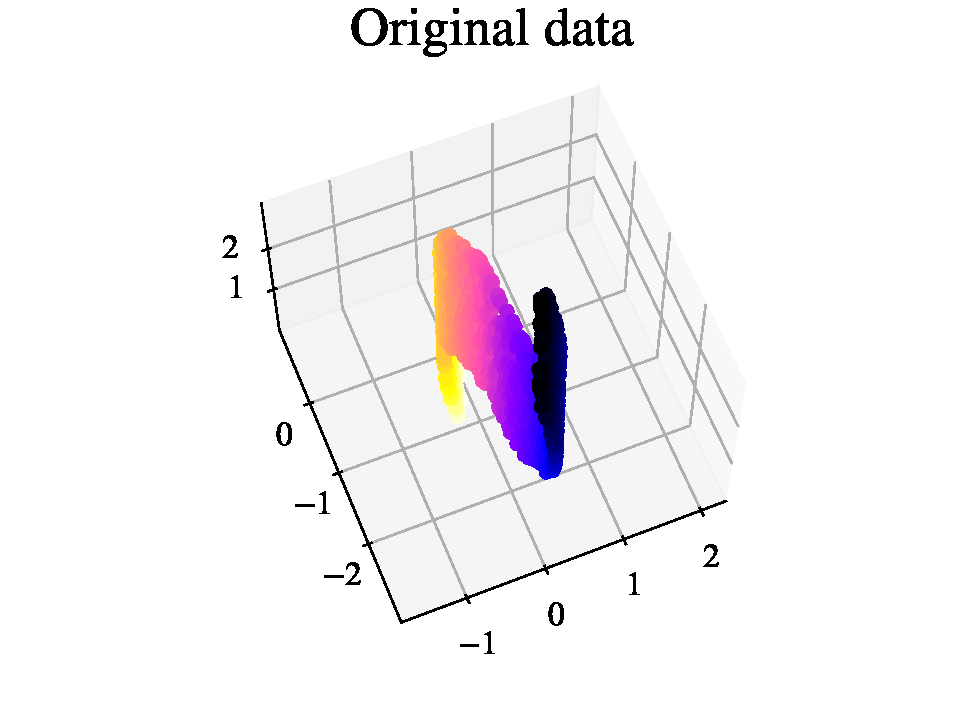
\includegraphics[width=7cm]{images/demo-structure-preservation/original-data.pdf}
        \hfill
        \\[\smallskipamount]
        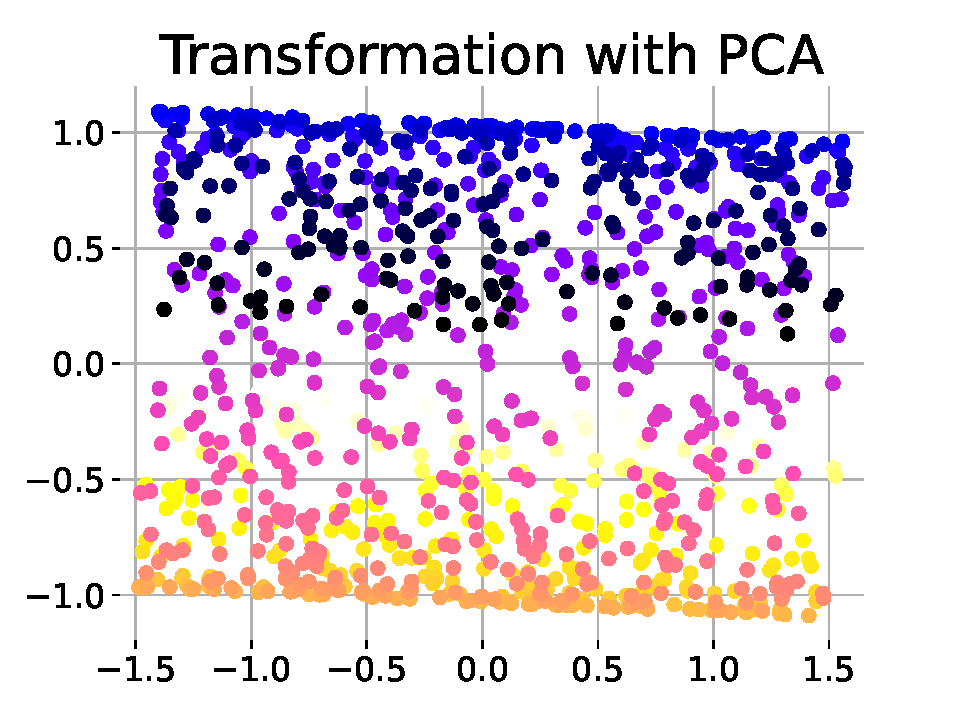
\includegraphics[width=6cm]{images/demo-structure-preservation/pca.pdf}\hfill
        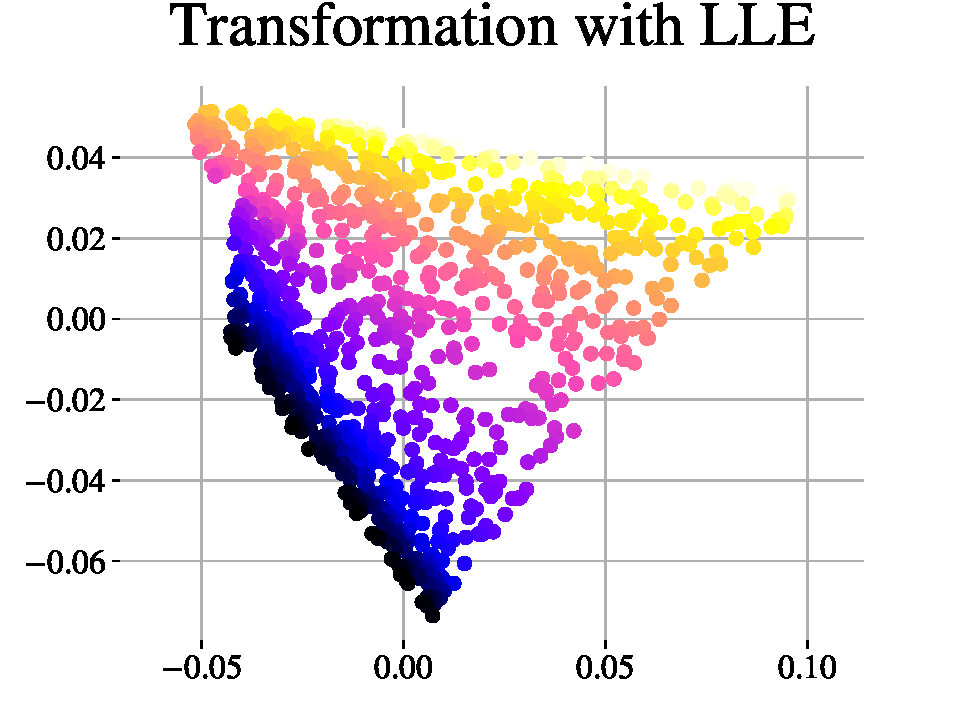
\includegraphics[width=6cm]{images/demo-structure-preservation/lle.pdf}
        \caption{Transformation results with different dimensionality reduction methods}
        \label{demo:structure-preservation}
    \end{center} 
\end{figure}
As a result, dimensionality reduction methods having both local and global structure-preserving properties, offer numerous advantages.
As mentioned above, the local structure-preserving property ensures that the fine-grained relationships within the data are captured in the lower-dimensional space.
Clusters, neighbourhoods or other local structures are therefore precisely represented.
On the other hand, dimensionality reduction methods with a high degree of global structure preservation maintain the overall relationships, dependencies and coherence of the data.
Thus the underlying data distribution is retained which helps with interpretability and visualisation.
Therefore combining both properties in a dimensionality reduction method enhances the representation of local details along with the global structure.

Figure \ref{demo:structure-preservation} shows the result of different dimensionality reduction methods on the same dataset.
This is an often-used example to visualise global and local structure preservation.
Here, the data is 3-dimensional and forms a S-shape.
As PCA reduces dimensionality by aiming at linear projections which maximise the global variance of the transformed data, it only considers the global structure but not the local structure \cite{global-local-structure} \cite{PCA-global-structure-preserving}.
Therefore the starting of the S is squashed with the middle part of the shape.
On the other hand, we see that LLE preserves the local structure, as only the nearest neighbours are close to each other in the transformation, while the distances to other data points are ignored.

Additionally to the above-mentioned structure preservations, we propose a new focus for dimensionality reduction methods. 
For instance for ordered data, like time series, it may be of importance that the distance between each data point and its sequential data point is maintained in the projected space.

\begin{definition}[Order-Based Distance Preservation]
    Let $X = (x_1,\dots,x_n )$ be an ordered dataset as sequences or set of sequences, see Section~\ref{ordered-data}.
    Furthermore, let $Y = (y_1, \dots, y_n)$ be its lower-dimensional projection by a dimensionality reduction method.
    We say the dimensionality reduction method aims to preserve the order-based distances if for every data-pair $(x_i, x_{i+1})$ for $ i \in \{1, \dots, n \}$ in the ordered data-set $X$, its respective lower-dimensional data-pair $(y_i, y_{i+1})$ has approximately the same distance in terms of a distance metric.
\end{definition}

\begin{figure}[htb!]
    \begin{center}
        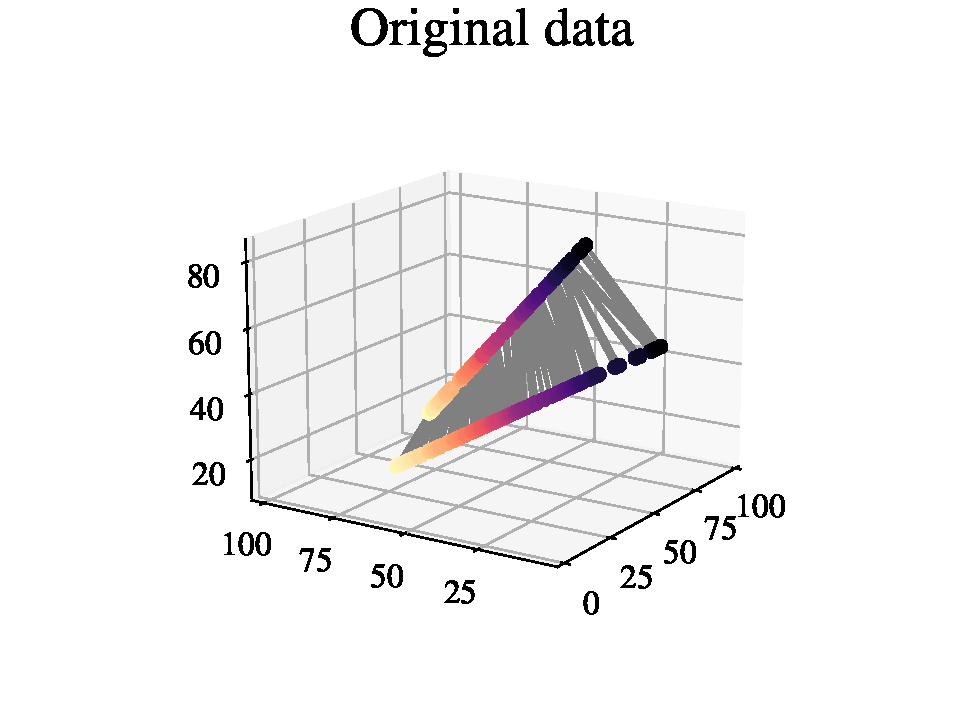
\includegraphics[width=7cm]{images/demo-structure-preservation/zigzag.pdf}
        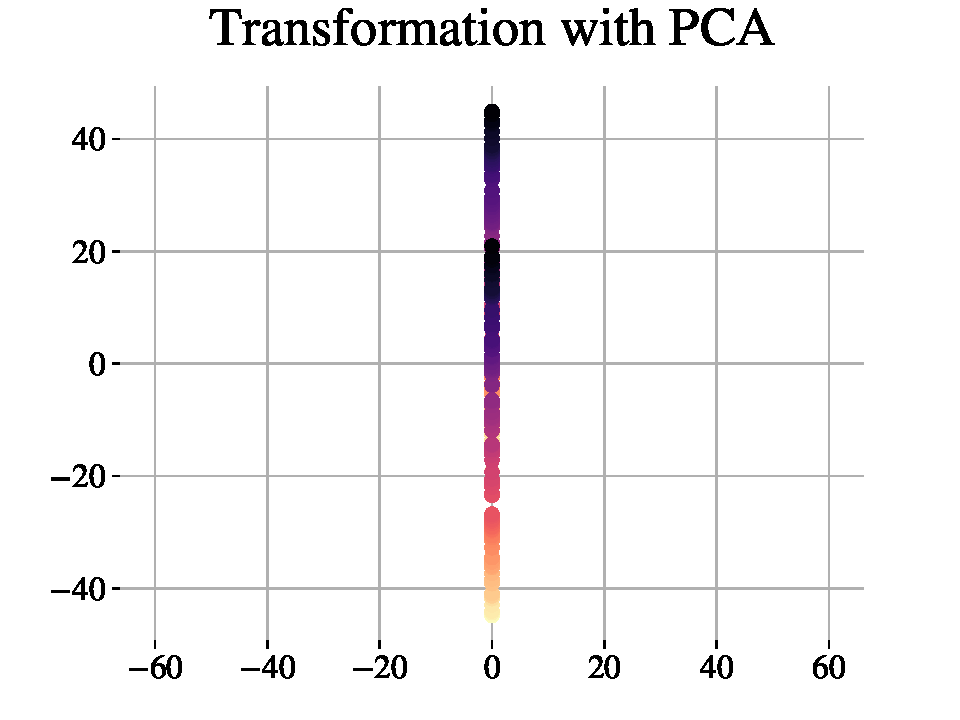
\includegraphics[width=6cm]{images/demo-structure-preservation/zigzag_pca.pdf}\hfill
        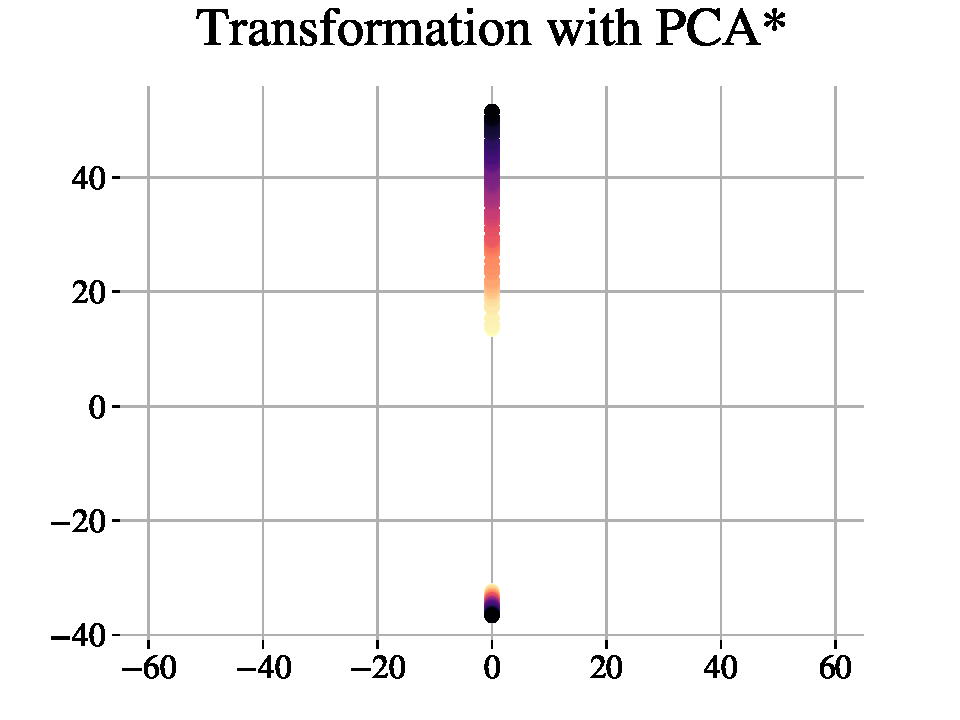
\includegraphics[width=6cm]{images/demo-structure-preservation/zigzag_vector.pdf}
        \caption{Transformation results with PCA and distance-order preserving variant PCA*}
        \label{demo:order-preservation-our}
    \end{center}
\end{figure}
Dimensionality reduction methods focusing on preserving order-based distances ensure that distances between each consecutive pair of data points in a sequence are similar in the original higher-dimensional and lower-dimensional space.
By preserving the distances in the order, the method can accurately capture sequential relationships.
This property is especially interesting for ordered data, where the order holds essential information like time series data.
This may improve the overall interpretability of the result as we assume that variables that are far away in an order are also less dependent in contrast to those which are close in the order.
See for example Figure~\ref{demo:order-preservation-our}.
The data points appear in two lines and are ordered in a zigzag form, meaning every next data point lies on the opposite line.
Transforming this data with PCA to a one-dimensional space, results in two lines but we see that the data points in the lines are not exactly as coloured as in the original space, whereas for the method PCA* they are.
PCA* is a variant of PCA, which focuses on preserving order-based distances.
For more information about PCA*, please refer to Section~\ref{pca*-section}.

One real-world example can be seen in genetic mutations which when appearing close to each other on a chromosome have a higher likelihood to be co-inherited compared to mutations which are positioned at a greater distance from each other \cite{order-important}.
Another example was shown by Advani, Papotti and Asudeh \cite{news-ordering} by demonstrating that among many other aspects, the order of how news appear on a web page or broadcasting service, may affect the readers' opinions about current events or other topics.
This can be manipulated in such a way that bias can be incorporated even though the correctness of the information is secured \cite{inject-bias}.

It is also important to note that achieving all three properties simultaneously can be challenging, as they sometimes conflict with each other.
For instance, retaining the local structure in a time series with rapid and large fluctuations may lead to distortions in the temporal order of the data points.
In other words, data points that were originally adjacent in time might have a different relationship with each other in the lower-dimensional representation to better satisfy the global distance preservation.


\section{Variants of Principal Component Analysis} \label{variants-pca}
With the motivation to find a dimensionality reduction method, which preserves order-based distances we chose PCA as our fundamental dimensionality reduction method due to its computational efficiency, deterministic results as well as its common usage in several fields \cite{pca-often}.
Thus, to incorporate sequential information into the dimensionality reduction technique we explore the following PCA variants: PCA with Ids, Complex PCA and PCA*.

\subsection{PCA with Ids} \label{subsec:idpca}
To answer the question of how we can insert structural information into the data to keep this information in the lower-dimensional representation, a common suggestion is, to enumerate the data points.
Assume $X$ to be the data conforming to the definition \ref{def:sequences} or definition \ref{def:set-sequences}.
To enumerate the data points, we add a new dimension with its enumerated ID value to each data point in $X$:
\begin{equation*}
    X = 
    \begin{pmatrix}
        x_{1,1} & \dots & x_{1,d} \\
        \vdots & \ddots & \vdots \\
        x_{n,1} & \dots & x_{n,d}
    \end{pmatrix}
    \rightarrow
    X_{\mathrm{id}} = 
    \begin{pmatrix}
        x_{1,1} & \dots & x_{1,d} & 1 \\
        \vdots & \ddots & \vdots & \vdots \\
        x_{n,1} & \dots & x_{n,d} & n
    \end{pmatrix}.
\end{equation*} 
There are two distinct approaches for the application of PCA to $X_{\mathrm{id}}$.
The first one is applying PCA on $X$ to compute the principal components, and then applying them to $X_{\mathrm{id}}$ on only the first $d$ entries to reduce the dimensionality.
This essentially gives the same representation to PCA with one dimensionality more, which contains the Id values.
When plotting the data, we have to either remove the dimensionality containing the enumeration and treat it as metadata, or if not, we have to plot a dimensionality more.
The other option is to apply PCA to the $X_{\mathrm{id}}$ as if the new extended dimension were a normal feature of the dataset.
In the subsequent, we explore some notable points why we have to be cautious when applying PCA on $X_{\mathrm{id}}$ to preserve order-based distances.
\paragraph{PCA on Discrete Data}
One assumption of PCA is that data follows a multivariate normal distribution, or at least, it operates under the assumption that the data is approximately normally distributed.
Discrete data, on the contrary, follows non-normal probability distributions \cite{pca-not-for-discrete}.
Therefore PCA treats the values in the Id dimension as numerical and may therefore attempt to find principal components that maximise variance in this dimension, which leads us to the next consequence.
\paragraph{Distortion of Order Distances}
As PCA aims to capture the most significant sources of variance, the presence of the enumeration dimension may lead PCA to emphasise variation that is unrelated to the order-based distances.
\paragraph{Loss of Interpretability}
The resulting principal components may not be easily interpretable, as the added dimension may dominate the principal components.
Therefore, extracting meaningful insights about the original order relationships is made difficult.


\subsection{Complex PCA on Ordered Data} \label{CPCA}
To address the challenge of order-based distance preservation in PCA, we augment the data with complex vectors derived from consecutive data points in the sequentially ordered data set.
Here we incorporate an additional layer of information that captures the sequential dependencies within the data in the complex part.
We start by computing for each data point the vector to the next data point in the sequence.
By adding the vectors as the complex part of the data, we aim to encode the sequential order effectively in the data itself.
Therefore, the real part of the augmented data retains the original data and the complex part denotes the inter-point relationships.
Applying principal components to the augmented data might thus lead to reduced information loss as the structure of the data is considered.

% Description
As described above, to incorporate the structure into the data, we exploit the complex space by adding imaginary values indicating the direction of the next data point:
\begin{align*}
    X & = 
    \begin{pmatrix}
        x_{1,1} & \dots & x_{1,d} \\
        \vdots &  \ddots & \vdots & \\
        x_{n,1} & \dots & x_{n,d}
    \end{pmatrix}
    \rightarrow \\
     X_{\mathrm{complex}} & =
    \begin{pmatrix}
        x_{1,1} + i c_{1,1} & \dots & x_{1,d - 1} + i c_{1,d - 1} & x_{1,d} \\
        \vdots &  & \vdots &\vdots & \\
        x_{n,1} + i c_{n,1} & \dots & x_{n,d - 1} + i c_{n,d - 1} &x_{n,d}
    \end{pmatrix},
\end{align*}
where each row of $X$ is a data point in $\R^d$ and $c_{k,l} = x_{k + 1, l} - x_{k,l}$ for $k \in \{1,\dots, n \}$ and $l \in \{1, \dots, d - 1\}$. 
When reducing the dimensionality of $X_{\mathrm{complex}}$ with PCA, we first have to centre the data.
If we centre the data, not considering the complex part as vectors, the vectors of the centred $X_{\mathrm{complex}}$ do not have the correct length to indicate the position of the next point:

\begin{leftbar}
    \textbf{Example} Assume the data to consist of three one-dimensional data points:
    \begin{equation*}
        \begin{split}
            x_1 = 1 \\
            x_2 = 3 \\
            x_3 = 7    
        \end{split}
        \quad\rightarrow\quad
        \begin{split}
            &x_{1, \mathrm{comp.}} = 1 + 2i \\
            &x_{2, \mathrm{comp.}} = 3 + 4i \\
            &x_{3, \mathrm{comp.}} = 7.
        \end{split}
    \end{equation*}
    Centring yields:
    \begin{align*}
        &x_{1, \mathrm{comp., centr.}} = -\frac{8}{3}  \\
        &x_{2, \mathrm{comp., centr.}} = -\frac{2}{3} + 2i \\
        &x_{3, \mathrm{comp., centr.}} = \frac{10}{3} - 2i.
    \end{align*}
    Thus we see, that the centred complex vectors do not have the correct length to accurately point to the next data point.
    Additionally, after centring, it becomes unclear where the sequence ends, since the last data point retains an imaginary part.
    This might be challenging when datasets consist of more than one sequence.
\end{leftbar}

As our primary motivation is to enhance the information of the data by incorporating the sequential vector data in the complex part, centring hinders this approach.
Hence we assume to only centre the data on the real part but leave the complex part.
This partial centring leads to the question if the result of complex PCA (CPCA) is still usable.
In \cite{uncentered-pca-burned} it is stated that centring data in SVD is optional and that not centring data minimises the influence of a cluster's variance on another cluster. 
Cadima and Jolliffe \cite{relation-centered-uncentered-PCA} show that the transformed columns of the $d$-dimensional data $X_{\mathrm{complex}} = X_{\mathrm{real}} + i X_{\mathrm{imag}}$ can be correlated and emphasise the difference of the principal components of centred and uncentred data:
Let $X_{\mathrm{complex}}\nu_i$ and $X_{\mathrm{complex}}\nu_j$ be transformed data, with $\nu_k$ being the $k$-th principal component of its respective eigenvalue $\lambda_k$ and $i,j,k \in \{1, \dots d\}$, then:
\begin{align*}
    \operatorname{Cov}(X_{\mathrm{complex}}\nu_i, X_{\mathrm{complex}}\nu_j) = \nu_i^T C \nu_j = \lambda_i \nu_i^T \nu_i - (\nu_i^Tc_m)(\nu_j^T c_m), 
\end{align*}
where $C$ is the covariance matrix of $X_{\mathrm{complex}}$ and $c_m = \frac{1}{n} \operatorname{Im}(X_{\mathrm{imag}})^T \mathbb{1}_n$.
This formula we already fit to our case with only the imaginary part not being centred.
We see in the equation, that if the principal components are uncorrelated depends on how far away the connected data points are.
Due to the resulting components potentially being correlated, they are generally dependent if the variables are Gaussian distributed.
As PCA is not suitable for dependent or correlated data, the result of this dimensionality reduction method might not be mathematically or statistically significant \cite{pca-only-independent}.
On the other hand, Joliffe states in \cite{PCA-joliffe} that uncentred PCA is a well-established method in chemistry, ecology and geology. 
They also mention that uncentred PCA performs eigenanalysis on matrices that are not covariance or correlation matrices but still can be seen as measures of similarity.

Apart from the above-shown consequences of partially centring data, applying PCA to $X_{\mathrm{complex}}$ introduces some other consequences.
Applying PCA to complex-valued data results in complex principal components which then transform into a lower-dimensional complex space, introducing a level of intricacies and the consideration of how the real and imaginary parts are interdependent, as these components are intertwined, especially during the process of finding the principal components of the covariance matrix $\operatorname{Cov}(X_{\mathrm{complex}})$:
\begin{align*}
    \operatorname{Cov}(X_{\mathrm{complex}}) \neq \operatorname{Cov}(X_{\mathrm{real}}) + \operatorname{Cov}(X_{\mathrm{imag}})
    ,
\end{align*}
where $X_{\mathrm{complex}} = X_{\mathrm{real}} + iX_{\mathrm{imag}}$.

In the following, we concentrate on two main variants of CPCA, as these maintain correctly scaled vectors directing to the next consecutive data point, which can be seen as metadata:
\begin{itemize}
    \item[] \textbf{CPCA-real}: After obtaining the complex principal components, we choose to focus only on the real part.
    \item[] \textbf{CPCA-imag}: To transform the complex data, we only use the imaginary part of the principal components.
\end{itemize}


Unlike PCA on real-valued data where the principal components are unique up to the sign, the principal components for PCA on complex data, or short Complex PCA (CPCA), are unique up to a multiplication by a unit phase factor $e^i\varphi$.
In the case of PCA, there are some commonly used options on how to ensure deterministic output:
One is the positive sign approach.
This simple and commonly used approach aligns principal components such that their signs are positive.
For example, we scale the vector in such a way, such that its maximum element is positive \cite{sign-flip}.
Another option is the largest-absolute-value-based approach.
This method ensures that the largest absolute value within each component is positive. This is also the approach we are using as \texttt{scikit} conforms to this as well, see \cite{sign-flip} and \cite{website-pca}.

The importance of choosing one convention to solve the sign arbitrariness can be seen in the comparison of results of multiple runs of PCA, see \cite{sign-flip}.

As the complex principal components are unique up to a scaling factor $e^i\varphi$, there are multiple ways to solve this ambiguity.
In the following, we explore two options:
\begin{itemize}
    \item \textbf{Align to PCA} To promote stability in the outcome of CPCA, we scale the complex principal components such that they are as close as possible to the principal components derived from applying PCA to the original data.
    The motivation behind this strategy is based on the desire to maintain the essence of the original data while leveraging the additional insights offered by the complex information.
    By aligning with the original principal components, we effectively 'ground' the complex principal components in a familiar, interpretable context, making them more accessible.
    Therefore, this alignment facilitates the interpretation of the result of CPCA in the context of the original data.
\end{itemize}
As the transformation with the resulting principal components of CPCA is complex, we may obtain the real part of the lower-dimensional representation.
Therefore, to not lose as much information, we explore the second option:
\begin{itemize}
    \item \textbf{Align to smallest imaginary part}
    By minimising the magnitude of the complex parts of the principal components, we effectively 'dampen' the influence of the phase information.
    This reduction in the complex part's magnitude aligns complex principal components more closely to their real counterparts.
    Therefore it promotes a deterministic and stable output, facilitating comparisons across different runs of complex PCA.
\end{itemize}

In the following theorem we show that phase-shifting a complex vector may not go as far as producing the exact same vector it has been aligned to:

\begin{theorem}[Unit Phase Factor Alignment] 
    The real part of a complex-valued vector cannot take any arbitrary value solely by unit phase factor alignment.
\end{theorem}

\begin{proof}
    Assume $x$ to be a complex vector.
    Let $\hat{x} = e^{i \varphi}x$ be the aligned vector obtained by aligning $x$ with a unit phase factor $e^{i \varphi}$.
    The real part of the aligned vector is given by $\operatorname{Re}(\hat{x}) = \operatorname{Re}(x) + \cos(\varphi) - \operatorname{Im}(x) \sin(\varphi)$ by using Euler's formula .
    Now assume there exists $Z \in \mathbb{R}$ arbitrarily chosen such that $\operatorname{Re}(\hat{x}) = Z$.
    With substituting this for $\operatorname{Re}(\hat{x})$, follows $\operatorname{Re}(x) \cos(\varphi) - \operatorname{Im}(x) \sin(\varphi) = Z$.
    This equation cannot be directly solved alone for $\varphi$ as it is also dependent on $\operatorname{Im}(x)$, $\cos(\varphi)$ and $\sin(\varphi)$.
    To prove this assume $x = 1$.
    Above equation is now $ \cos(\varphi)= z$.
    Since $\cos(\varphi)$ is bounded between $-1$ and $1$, $z$ can only take values between $-1$ and $1$.
    Now consider $x = i$ which is purely complex.
    This makes above equation $\operatorname{Re}(0) \cos(\varphi) - \operatorname{Im}(i) \sin(\varphi) = Z$.
    Therefore $-\sin(\varphi) = Z$.
    As $\sin()$ is bounded, $Z$ cannot be arbitrarily chosen in $\mathbb{R}$.
\end{proof}

In summary, we see that incorporating the sequential information into the data as the complex part to maximise the degree of how well PCA maintains the order-based distances within the data, has some disadvantages, like resulting dependence in data, phase aligning and poorer interpretability.

\subsection{PCA*} \label{pca*-section}
This chapter introduces a variant of Principal Component Analysis that leverages the concept of vector differences between consecutive points in the dataset, allowing for the analysis of sequential changes and trends in the data.
Principal Component Analysis for Structure-Aware Representation (PCA*) focuses essentially on the connections of each pair of consecutive data points in the sequentially ordered dataset.

\begin{definition}[PCA*] \label{pca*}
    Assume a high-dimensional dataset $X \subset \mathbb{R}^{n \times d}$ consisting of $n$ $d$-dimensional data points $\{x_1, \dots, x_n \} $.
    To transform the data with PCA* following steps have to be taken:
    \begin{enumerate}
        \item Data Centering: Data centring is done by subtracting the mean of each column from the corresponding column of the data matrix $X$. \label{cent-data}
        Let $\mu_X$ be the set of all means in $X$ and $X_\mathrm{centred}$ be the computed centred dataset.
        This step is important as without it the result may be shifted, see the general case in Theorem~\ref{data-uncentred}.
        \item Vector Computation: Compute the connections of each consecutive pair of data points in $X$. \label{vector-comp}
        Let $V = \{v_1, \dots, v_{n-1} \}$ be the set of all these vector differences, with
        \begin{align*}
            v_i = x_{i+1} - x_i \text{   } \forall i \in \{1, \dots, n-1\}.        
        \end{align*}
        \item Vector Centring:
        As we have seen in the previous subsection, centring data before applying SVD is crucial.
        Therefore, $V$ needs to be centred similarly to step 1.
        Denote $V_\mathrm{centred}$ as the centred $V$.
        \item SVD Decomposition: Next perform Singular Value Decomposition (SVD) on $V_\mathrm{centred}$.
        SVD decomposes $V_\mathrm{centred}$ into three matrices:
        \begin{align*}
            V_\mathrm{centred} = U \Sigma Z^T,
        \end{align*}
        where 
        \begin{itemize}
            \item $U$ contains the left singular vectors
            \item $\Sigma$ is a diagonal matrix containing singular values
            \item $Z^T$ is a transposed matrix consisting of right singular vectors.
        \end{itemize}
        \item Selecting Principal Components: We sort the singular values in $\Sigma$ in descending order.
        The principal components corresponding to the largest singular values capture the most variance in the data $V$.
        Thus, we choose the top $k$ principal components, where $k$ denotes the desired number of dimensions for the lower-dimensional space.
        Let $PC_k$ be the matrix containing the chosen principal components as columns.
        \item Projection: Using the principal components from the step earlier, we project $X_\mathrm{centred}$ into the lower-dimensional space:
        \begin{align*}
            X_{\mathrm{transf}} = X_\mathrm{centred} PC_k.
        \end{align*}
        \item Reconstruction [Optional]: We reconstruct the lower-dimensional representation of $X$ back into the original high-dimensional space:
        \begin{align*}
            X_{\mathrm{reconstr}} = X_{\mathrm{transf}} PC_k^T + \mu_X,
        \end{align*}
        where $PC_k^T$ denotes the transposed matrix $PC_k$ and $\mu_X$ be the column-wise mean of $X$ of step 1.
    \end{enumerate}
\end{definition}

By focusing on the connections between sequential data points and by applying PCA to them, PCA* aims to capture the most important directional changes in the data while reducing dimensionality.

\begin{theorem} \label{data-uncentred}
    Let $X$ be the original high-dimensional source data and let $PC_k$ be the top $k$ principal components corresponding to the largest eigenvalues of the SVD of $X_{\mathrm{centred}}$, where $X_{\mathrm{centred}}$ denotes the centred data $X$, like in the Definition~\ref{pca*} of PCA* in step \ref{cent-data}.
    Not centring the original data when applying the principal components $PC_k$ may result in shifted reconstructed data for PCA and PCA*.
\end{theorem}

\begin{proof}
    Assume $X$ to be the source data.
    We now want to show that if we compute PCA on the centred data $X_\mathrm{centred}$ and then apply the principal components to $X$, the resulting data is shifted.
    Suppose $PC = \{pc_1, \dots, pc_d\}$ are the principal components calculated by applying PCA to the centred data $X_\mathrm{centred} = X - \mu_X$, where $\mu_X$ the column-wise mean denotes.
    We now transform both $X$ and  $X_\mathrm{centred}$ with a subset of $PC$ of vectors corresponding to the biggest eigenvalues $PC_k$, where $k$ denotes the number of dimensions of the lower-dimensional space.
    Originally PCA applies the principal components onto $X_\mathrm{centred}$:
    \begin{align*}
        X_{\mathrm{centred, transf}} = X_\mathrm{centred} PC_k.
    \end{align*}
    We now want to check applying the principal components on $X$:
    \begin{align*}
        X_{\mathrm{transf}} = X PC_k.
    \end{align*}
    We now can substitute $X$ with $X_\mathrm{centred}$:
    \begin{align*}
    X_\mathrm{transf} = X PC_k = (X_\mathrm{centred} + \mu_X) PC_k.
    \end{align*}
    Therefore the transformation does not eliminate the mean contribution from the data and the resulting transformed data may not have a mean of zero.
    When reconstructing the data we see the shift even more:
    \begin{align*}
        \begin{split}
            X_\mathrm{reconstr} & = X_\mathrm{transf} PC_k^T = (X_\mathrm{centred} + \mu_X) PC_k PC_k^T \\ & =  X_\mathrm{centred} PC_ PC_k^T + \mu_X PC_k PC_k^T
        \end{split}
    \end{align*}
    whereas for the centred data follows:
    \begin{equation*}
        \begin{split}
            X_{\mathrm{centr, reconstr}} & = X_{\mathrm{centr, transf}} PC_k^T = X_\mathrm{centred} PC_k PC_k^T,
        \end{split}
    \end{equation*}
    where then PCA adds $\mu_X$ to shift the reconstructed data to the centre of $X$, in contrast to the uncentred case where $\mu_X P C_k P C_k^T$ is added but this is not the correct centre of $X$.
    Thus the reconstruction of the uncentred data appears shifted.
\end{proof}
\begin{figure}[htb!]
    \subfigure[Data with high fluctuations]{
        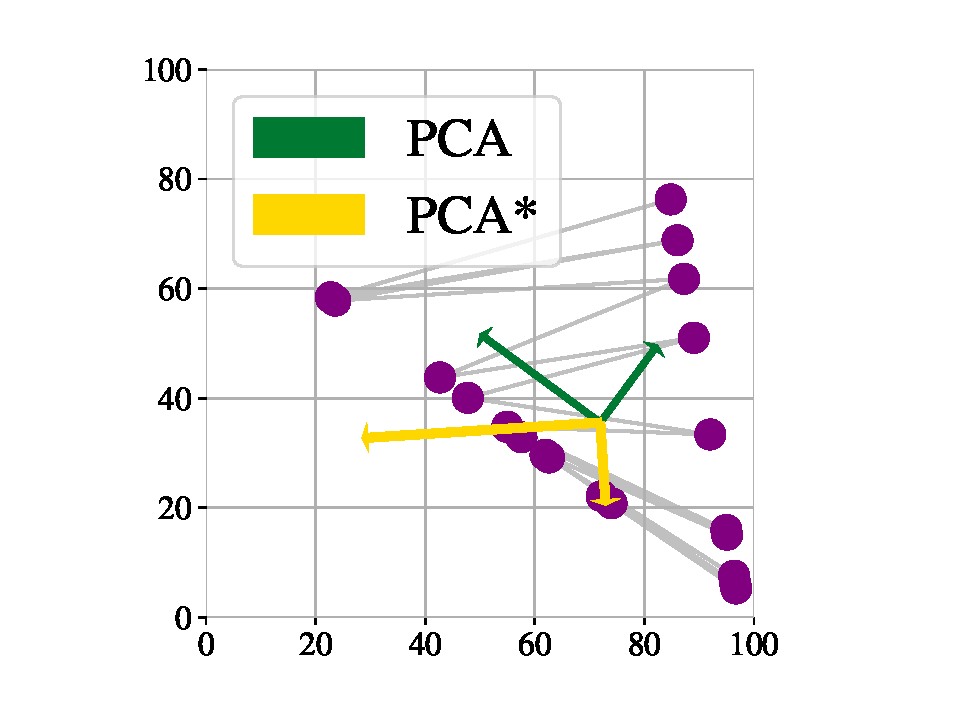
\includegraphics[width= \textwidth /2]{images/pcastar/zigzag.pdf}}
    \subfigure[Data with low fluctuations]{
        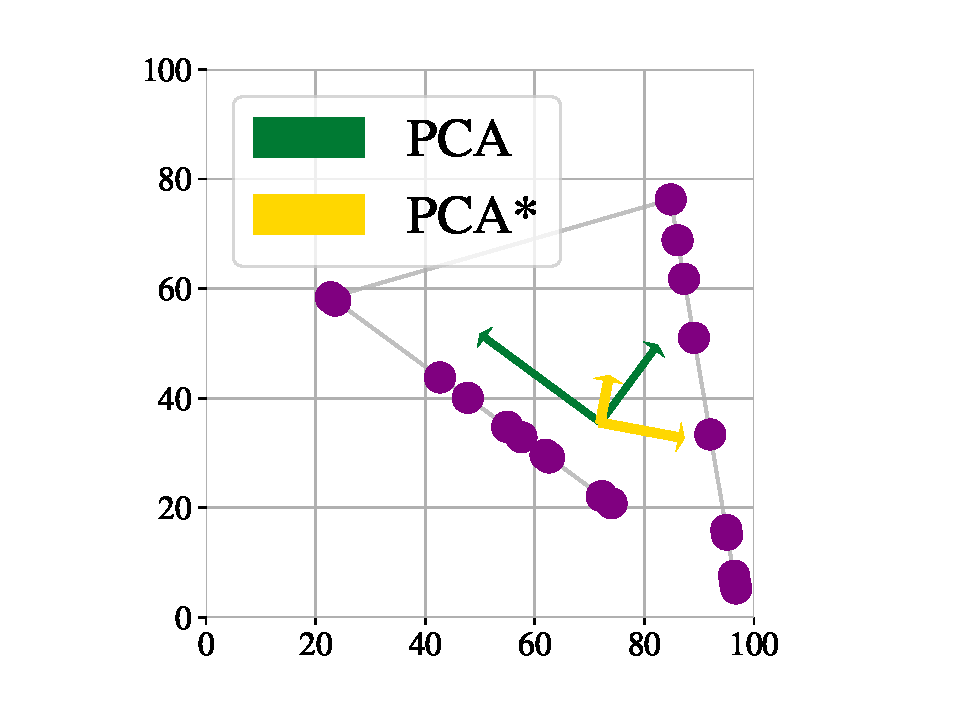
\includegraphics[width= \textwidth /2]{images/pcastar/one_line.pdf}}
    \caption{Principal components for PCA and PCA* on differently ordered datasets}
    \label{fig:pcs-difference}
\end{figure}
As PCA and PCA* might look similar we now explore their main differences:
\begin{enumerate}
    \item Data Representation:
    \begin{itemize}
        \item PCA: PCA operates on tabular data, where each row represents an observation and each column a feature.
        It aims to find orthogonal linear combinations of the original features to project the data into a new lower-dimensional space while still maximising the variance.
        \item PCA*: PCA* is specifically designed for sequential data, where each data point is a vector observed over time or multiple sequences of vectors observed over time.
        It focuses on preserving the sequential relationships within the data while reducing dimensionality.
    \end{itemize}
    \item Dimensionality Reduction Goal:
    \begin{itemize}
        \item PCA: PCA aims to reduce the dimensionality of data by finding a new set of orthogonal axes that capture the maximum variance.
        It assumes the data points to be independent and does not consider any inherent time or sequential order.
        PCA treats each data point as a separate entity.
        \item PCA*: On the other hand, the primary goal of PCA* is to reduce dimensionality while still preserving the temporal or sequential relationships within the data.
        To accomplish this PCA* looks for a lower-dimensional representation that maintains the underlying patterns and dependencies in the data.
        It therefore might happen that the same data just differently ordered results in different lower-dimensional representations, see Figure~\ref{fig:pcs-difference}.
    \end{itemize}
    \item Applications:
    \begin{itemize}
        \item PCA: This is an often used dimensionality reduction method for various tasks, like feature selection, noise-reduction and visualisation of high-dimensional data.
        \item PCA*: PCA* is a specifically tailored algorithm for tasks like data analysis, where the sequential order of observations is crucial.
    \end{itemize}
\end{enumerate}

Figure \ref{fig:pcs-difference} emphasises the different results of PCA* and PCA.
While PCA finds for both orders the same principal components, PCA*'s principal components depend on the order.
Thus it provides a more flexible approach to dimensionality reduction, as it acknowledges that different orders and sequences within the data may reveal distinct patterns.

To summarise: PCA is a general-purpose dimensionality reduction method, whereas PCA* focuses on sequential data analysis, enhancing the quality of sequential dependencies within the data points.


\chapter{Experiments}\label{experiments}
In this chapter, we present a series of experiments to evaluate PCA* and the CPCA variants.
We begin by introducing the data used for these experiments, which include both synthetic, generated data and real-world data such as stock closing prices.
To assess the results, we use quality measures outlined in the second section of this chapter.
While there are several variants of PCA discussed in Section~\ref{variants-pca}, our primary focus in this section lies on PCA*.
However, we also explore some of the primary experiment settings involving these CPCA variants.
The measures are used to compare PCA* to some of the most often used dimensionality reduction methods described in Chapter~\ref{related-work}, namely PCA, LLE, UMAP, t-SNE. 

\section{Datasets} \label{datasets}
To evaluate the dimensionality reduction methods, we explore multiple generated and real-world datasets.
We first describe how we generate data and subsequently examine datasets of stock closing prices, air pollution in Japan and generated flight data (MTS).

\paragraph{Synthetic Data} \label{generated_data}
These data we constructed to assess and compare the performance of PCA*, Id PCA and the CPCA variants against other common dimensionality reduction methods on data where we have control over their complexity and order.
The data generation process involves constructing data points that lie consecutively on $l$ lines within a high-dimensional space.
These lines are then sorted, so that the starting and ending points of close lines are near in proximity.
Each line consists of an equal number of data points.
To obtain sequentially ordered data, as defined in Section~\ref{ordered-data}, we shuffle the data points to resemble specific orderings.
These can be categorised as zigzag and smoothly ordered data as well as data ordered in separate lines.

\begin{figure}
    \subfigure[Zigzag order]{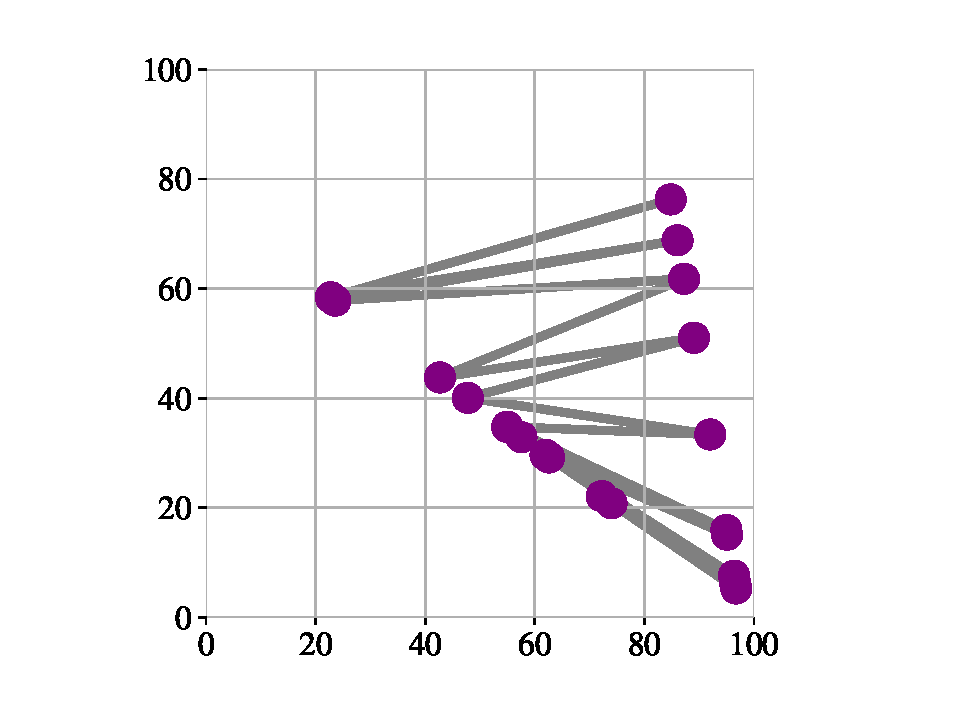
\includegraphics[width=\textwidth / 4]{./images/demo_orders/zigzag.pdf} \label{zigzag}}
    \hfill
    \subfigure[Smooth order]{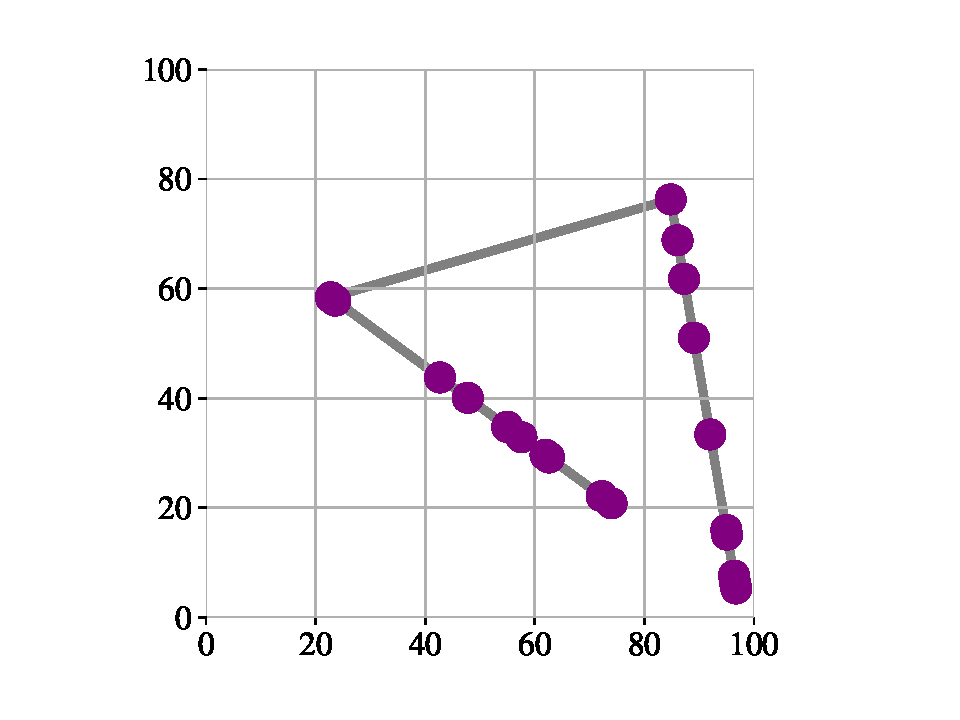
\includegraphics[width=\textwidth / 4]{./images/demo_orders/one_line.pdf} \label{one-line}}
    \hfill
    \subfigure[Separate lines]{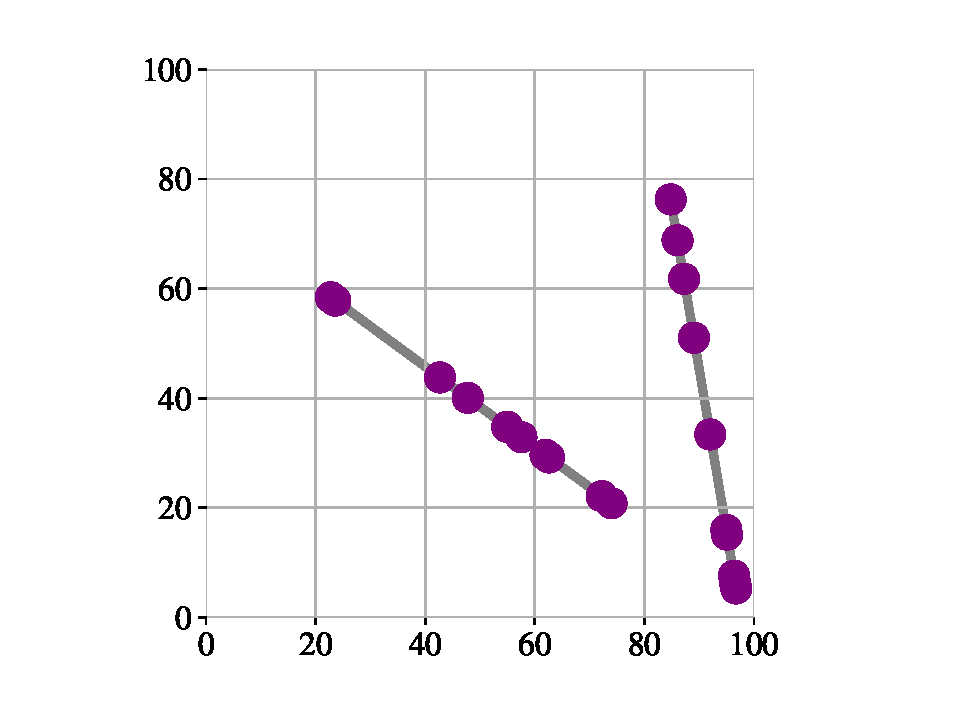
\includegraphics[width=\textwidth / 4]{./images/demo_orders/sep_lines.pdf} \label{sep_lines}}
    \hfill
    \caption{Figures show two-dimensional data generated in two lines.}
\end{figure}
If the data is arranged in zigzag order, we order the data points by their position within the lines.
Suppose a list of lines.
We then collect iteratively the $i$th points of each line:
we start by taking the first points of each line, then the second until all points are collected.
This creates a zigzag pattern as seen in Figure~\ref{zigzag}.

However, if the order of the data is smooth, then we connect each separate line by a continuous line.
If we desire the data to remain in separate lines, we refrain from connecting them.
An example is given in Figure~\ref{ordered-data}, where \ref{zigzag} how the data is ordered in a zigzag form, \ref{one-line} shows the same data as one-line ordered data and finally \ref{sep_lines} the data as separate lines.
We selected these orderings to simulate different data behaviours.
Zigzag-ordered data represent data which have rapid and high fluctuations, while smoothly-ordered data simulates datasets where consecutive data points change only gradually.
To cover a range of scenarios, we explore data ordered in separate lines.
All these data orders consist of the same data points, allowing us to evaluate the effect of different ordering patterns on the performance of various dimensionality reduction methods.

We also introduce a level of randomness by adding a random value within a range determined by a jitter-bound to each dimensionality in the generated data points.
This introduces slight variations in the data, making it more representative of real-world scenarios where data may not be perfectly precise but can exhibit small fluctuations.

\paragraph{Simulated and Real-World Data} \label{real-world-data}
As the synthetic data consists of data points laying on more or less straight lines, we also explore PCA* on bigger datasets, and compare the results with the outcomes with PCA, LLE, t-SNE and UMAP:
\begin{itemize}
    \item \textbf{Russell2000} The Russell2000 data consists of daily adjusted close prices of 1794 stocks like the CCBG (Capital City Bank Group, Inc.) and HCT (Holista Colltech Limited) for the time of January 1st, 2013 to 2014 \cite{russell2000}.
    For simplicity, we excluded stocks containing missing data and omitted the time dimension since the order of the data points is represented by their input sequence.
    Thus, our analysis is conducted on a 1597-dimensional dataset, with each dimension containing 504 numerical observations.
    \item \textbf{MTS} We utilise the data set sourced from NASA \cite{mts-flights}, containing 10 samples of flight data.
    The dataset, although valuable for our purposes, presents certain limitations.
    Specifically, apart from basic information such as data sizes and dimensions for each flight time series, no additional contextual details were provided.
    However, these limitations do not hinder our primary research objective, which focuses on testing and evaluating dimensionality reduction techniques with respect to order-based distance preservation.
    Each of the given flight data contains 30 dimensions of which one denotes the time, which we removed similarly to the Russell2000 data.
    The number of observations varies between 4660 and 4900.
    To make them all equally long, we shortened each time series to 4660 data points.
    \item \textbf{Air Pollution in Japan} This air pollution dataset consists of observations of the nationwide sensor network surveilling air pollution in Japan, called the Atmospheric Environmental Regional Observation System (AEROS), set up by the Ministry of Environment Japan.
    There are hourly recordings of more than a thousand sensors from 2018 to 2023.
    Missing values are substituted with zeroes as recommended by the authors.
    Overall the dataset contains 1832 dimensions \cite{air_pollution}.
    In this thesis, we use the data from the first half year which contains 4380 observations.
\end{itemize}

As a result, these datasets exhibit diverse characteristics:
One dataset features more dimensions than observations, another has low dimensions but a substantial number of observations and is ordered in separate flights, and the final dataset combines high dimensions with a large number of observations.

\section{Quality Measures for Dimensionality Reduction Algorithms} \label{quality-measures}
In order to evaluate the effectiveness of dimensionality reduction techniques, we need some measures for datasets to quantify the dissimilarity between the transformed data and the original dataset.
We first discuss two fundamental metrics Mean Absolute Error (MAE) and Root Mean Square Error (RMSE).
These metrics provide insights into the average distances between corresponding data points in two datasets.
Based on these two metrics, we explore two new metrics which are used to assess the performance of dimensionality reduction methods.
Finally, we explore the Dynamic-Time Warping Algorithm and how we can use it to compare patterns in two data sequences.

In this section, we assume data to be sequential if not other stated.
The next definition is based on \cite{error-measures}.
\begin{definition}[Mean Absolute Error]
    The mean absolute error (MAE) measures the average absolute distances between two equally large sets of data $X$ and $Y$.
    It is computed by summing up the absolute distance between each dataset and then dividing it by the total number of values.
    More precisely:
    \begin{align*}
        \operatorname{MAE}(X, Y) = \frac{1}{n} \sum_{i=1}^n \| x_i - y_i \|,
    \end{align*}
    where $\| \cdot \| $ is the $L_2$-norm and for $x_i \in X$ and $y_i \in Y$ for $i \in \{1, \dots, n \}$. $n$ is the number of observations.
\end{definition}
The mean absolute error is a metric used to quantify the average magnitude of errors between two sets of values.
In simpler terms, MAE measures the average distance between data points of $X$ and $Y$, with no consideration of the direction of the errors.
Lower MAE values indicate higher similarity as they imply a smaller average deviation between each observation.
The following definition is based on \cite{error-measures}.
\begin{definition}[Root Mean Square Error]
    The root mean square error (RMSE) is a measure to compute the distance of two datasets $X$ and $Y$ with $n$ entries.
    It is calculated by taking the square root of the average of the squared distances between $X$ and $Y$:
    \begin{displaymath}
        \mathrm{RMSE}(X,Y) = \sqrt{\dfrac{1}{n} \sum_{i = 1}^{n}(x_i - y_i)^2},
    \end{displaymath}
    where $x_i \in X$ and $y_i \in Y$ for $ i \in \{1, \dots, n \}$ and $n$ is the number of observations.
\end{definition}
RMSE measures the square root of the average of the squared errors, giving more weight to larger errors compared to MAE.
Similarly to MAE, lower RMSE values indicate more similar datasets.

The next measure was proposed by Hajizadeh, Aghagolzadeh and Ezoji (2020) \cite{distance-measure}.
Unlike suggested in the paper, we do not scale with the proposed scaling factor to compare the higher- and lower-dimensional spaces, as the lower-dimensional representation is directly projected onto the higher-dimensional space without any change in the length of the data vectors, see following theorem:
\begin{theorem} \label{inv-transf-length}
    Let $X$ be a $d$-dimensional data with $n$ data points and let $X_{\mathrm{transf.}}$ be its PCA-transformed lower-dimensional representation.
    Then points in the transformed dataset have the same length as their respective points in the reconstructed embedding.
\end{theorem}

\begin{proof}
    Assume $y = (y_1, \dots, y_k) \in \R^k$ to be the transformed version of a data point in $X$ where $k \leq d$.
    We can rewrite the inverse-transformed $y$ as follows:
    \begin{align*}
        (y_1, \dots, y_k) 
        \begin{pmatrix}
            \nu_{1,1} & \dots & \nu_{1,d} \\
            \vdots & \ddots & \vdots \\
            \nu_{k,1} & \dots & \nu_{k,d}
        \end{pmatrix}
        & = \left( \sum_{i=1}^k y_i \nu_{i,1}, \dots, \sum_{i=1}^k y_i \nu_{i,d} \right) \\
        & = \sum_{i = 1}^k y_i (\nu_{i,1}, \dots, \nu_{i,d}) \\
        & = \sum_{i = 1}^k y_i \nu_i,
    \end{align*}
    where $\nu_i = (\nu_{i,1}, \dots, \nu_{i,d}) \in \R^d$ denote the principal components with $i \in \{1, \dots, k\}$.
    With this, we show that the reconstructed point has the same length:
    \begin{align*}
        \norm{\sum_{i = 1}^k y_i \nu_i} ^2 
        & = \Biggl \langle \sum_{i = 1}^k y_i \nu_i, \sum_{i = 1}^k y_i \nu_i  \Biggl \rangle \\
        &=  \sum_{i=1}^k \sum_{j=1}^k y_i y_j \underbrace{\langle \nu_i, \nu_j \rangle}_{\substack{= 0, \text{ if } i \neq j \\ = 1, \text{ if } i = j}} \\
        & = \sum_{i=1}^k y_i^2 \\
        & = \| (y_1, \dots, y_k) \|^2,
    \end{align*}
    where we used $\| \cdot \|^2 = \langle \cdot, \cdot \rangle$ with the scalar product $ \langle \cdot, \cdot \rangle$.
\end{proof}
In other words, if we initially had data in a 100-dimensional space and reduced it to a 2-dimensional representation using PCA, the reconstructed data points form a 2-dimensional plane in the 100-dimensional space.

\begin{definition}[Neighbour-Distance-Measure] \label{Neighbour-Distance-Measure}
    Let $X = (x_1, \dots, x_n)$ and $Y=(y_1, \dots, y_n)$ be two datasets that may not have the same dimensions.
    The Neighbour-Distance-Measure is the RMSE of distances between each successive point in $X$ subtracted by the respective distance by each point in $Y$:
    \begin{align*}
        q_{\mathrm{neigh-distance}} (X,Y) = \frac{1}{nk} \sum_{i=1}^n \sum_{{j=1}}^k \left| \|x_i - x_j\|^2 - \|y_i - y_j\|^2 \right|,
    \end{align*}
    where $\| \cdot \|$ is the $L_2$-norm and $k$ is the number of nearest neighbours of a point $x$ in $X$, see Definition~\ref{kNN}.
\end{definition}
As we are not operating on a dataset, but rather a data sequence we are not considering the $k$-nearest spatial neighbours but rather the $k$-nearest neighbours on the sequence.

The Neighbour-Distance-Measure quantifies how similar pairwise distances between data points in two datasets are.
This is done by comparing the squared distances between successive points in dataset $X$ to the corresponding squared distances in dataset $Y$.
Therefore, it is important to note that this measure relies on the method of how the neighbouring data points are sampled.
A lower value of the Neighbour-Distance-Measure indicates a higher similarity in the datasets.

As the Neighbour-Distance-Measure compares how the pairwise distances in each data set differ from each other, we define our second measure to evaluate the relation between each data point to its neighbouring point in both datasets.
\begin{definition}[Neighbour-Relation-Measure]
    Consider the dataset $X = (x_1, \dots, x_n)$ in $d$-dimensional space and its projection $Y = (y_1, \dots, y_n)$ in lower-dimensional space with $k$ dimensions where $k < d$.
    Let $V = (v_1, \dots, v_{n-1})$ represent the vectors connecting each data point to its successive data point:
    \begin{align*}
        v_i=x_{i+1} - x_i \text{   } \forall i \in \{1, \dots,n-1\}.
    \end{align*}
    Let $U = (u_1, \dots, u_{n-1})$ be the corresponding list of vectors for the projected data $Y$. The neighbour-relation measure quantifies the similarity between the relationships of vectors $V$ and $U$ as follows:
    \begin{align*}
        q_{\mathrm{scal-prod}} (X,Y) = \frac{1}{n-2}\sum_{i=1}^{n-2} |\langle v_i,v_{i+1} \rangle - \langle u_i,u_{i+1} \rangle|,
    \end{align*}
    where $\langle \cdot \rangle$ denotes the standard scalar product.
\end{definition}
% We have n - 2 many absolute values we sum up, as the formula for finding the possible number of consecutive elements in a sequence is n - k + 1.
% We have only n -1 vectors and consider two elements to be consecutive -> (n - 1) - 2 + 1= n - 2
As this measure uses the scalar product of the connections between each data pair in a sequence, we may call it the scalar-product measure as well.

Similarly to the neighbour-distance measure above we can extend the neighbour-relation measure to multiple neighbours, to see if the relation up to the next $k$ neighbours stays the same.

\begin{definition}[Multiple-Neighbour-Relation-Measure] \label{Multiple-Neighbour-Relation-Measure}
    Let $X = (x_1, \dots, x_n)$ be the data in a $d$-dimensional space and $Y = (y_1, \dots, y_n)$ its dimensionality reduced or reconstructed representation.
    To measure the relation up to $k$ neighbours, we sum the neighbour-relation measure up for every k-nearest neighbour on the sequence and take the mean:
    \begin{align*}
         q_{\mathrm{mult-scal-prod}} (X,Y) =
        \frac{1}{\sum_{l = 1}^k (n - 2l)} \sum_{j=1}^{k} \sum_{i = j + 1} ^{n-j} |\langle v_{i,j}^-,v_{i,j}^+ \rangle - \langle u_{i,j}^-,u_{i,j}^+ \rangle|,
    \end{align*}
    where $v_{i,j}^-$ represents the vector from the $i$th point to its $j$th predecessor, while $v_{i,j}^+$ represents the vector between the $i$th point to its $j$th successor.
    Similarly, $u_{i,j}^-$ and $u_{i,j}^+$ denote the corresponding vectors in the original data.
    Moreover, $k < n / 2$ denotes the number of considered nearest data points on the order of $X$ and $\langle \cdot, \cdot \rangle$ the standard scalar product.
\end{definition}

In essence, this measure computes the MAE of the differences between the pairwise scalar products of the vectors.
Therefore we not only compare the length of each connection between the data-pairs in the order of the data, but also quantify the angle between them.
\begin{wrapfigure}{r}{7cm}
    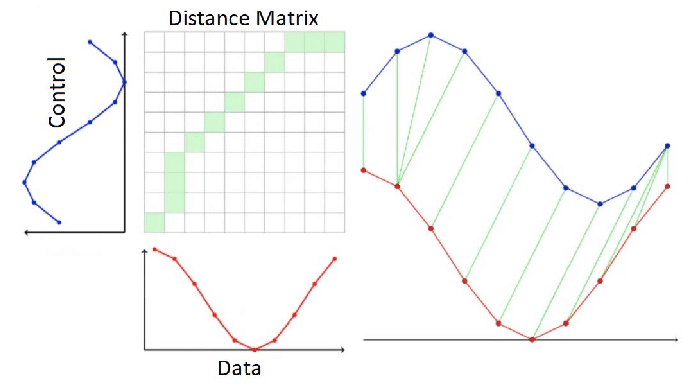
\includegraphics[width=7cm]{images/Dynamic-Time-Warping-23.png}
    \caption{Dynamic Time Warping by Diab Mahmoud Diab, Basil AsSadhan, Hamad Binsalleeh, S. Lambotharan, Konstantinos Kyriakopoulos, and Ibrahim Ghafir \cite{dtw-image}}\label{wrap-fig:1}
\end{wrapfigure} 
A lower error implies that the dimensionality reduction technique maintained the essential structure and patterns in the data, as the Scalar-Product-Measure takes the angle between each connection into account as well as both lengths of the vectors between the two data points.

As time series data play in many data science and data mining fields an important role, the need to compare time series increased.
One often used time series similarity measure is the Dynamic Time Warping (DTW) algorithm.
DTW was introduced by Berndt and Clifford in 1994 to find similarities in time series, as it was earlier used in the speech recognition field \cite{introduction-dtw}.
It aims to capture patterns and similarities in two sequences by minimising the cumulative distance along an optimal alignment path that matches corresponding data points while keeping the influence of temporal shifting and distortion low.
The next definition is sourced from \cite{weighted-dtw} and \cite{scaling-dtw}.
\begin{definition}[Dynamic Time Warping] \label{dtw}
    Let $X = (x_1, \dots. x_n)$ be a sequence of $n$ $d$-dimensional data points and $Y = (y_1, \dots, y_m)$ be a second sequence of $m$ $d$-dimensional data points.
    The first step to compute Dynamic Time Warping algorithm (DTW) is to calculate the $n \times m$-dimensional distance matrix $\operatorname{Dist}_{X, Y}$ of $X$ and $Y$ where the $(i^{th}, j^{th})$ entry of $\operatorname{Dist}_{X, Y}$ equals the squared distance of $x_i$ and $y_j$.
    $Dist_{X, Y}$ is also sometimes called path matrix as it is used to find the best warping path between these sequences which minimises the total cumulative distance between them.
    A warping path $P = (p_1, \dots, p_k)$, where $\max (m, n) \leq k < m + n - 1$ and $p_l$ being a entry of $\operatorname{Dist}_{X, Y}$, is a set of matrix entries defining a mapping between $X$ and $Y$ with following constraints:
    \begin{itemize}
        \item Endpoint constraint: the start- and endpoints of the warping path have to be the first and last data points of the path matrix, meaning $p_1 = (x_1, y_1)$ and $p_k = (x_n, y_m)$.
        \item Continuity constraint: The path cannot skip a step, i.e. the path takes step after step.
        This is when for the step $p_k = (x_i, y_j)$ and its following step $p_{k + 1} = (x_{i + 1}, y_{j + 1})$ where $x_i - x_{i +1} \leq 1$ and $y_j - y_{j + 1} \leq 1$.
        \item Monotonicity: the path is increasing, meaning the indices in the path move forward or stay the same while traversing the path.
    \end{itemize}
    Let $\mathcal{P}$ be the set of all warping paths $P$ mapping between $X$ and $Y$ as described above.
    DTW aims to minimise the warping costs:
    \begin{align*}
        \operatorname{DTW}(X, Y) = \min_{P \in \mathcal{P}} \Bigl \{ \sum_{p \in P} p \Bigr \}. 
    \end{align*}
    
    Two sequences are optimally matched with the lowest distance path.
\end{definition}

DTW captures patterns and similarities in sequences which might have different lengths, speeds or temporal distortions.

In this work, we focus on the first two measures we explored: the Neighbour-Distance Measure and the Neighbour-Relation Measure, as these two are specifically created to quantify the order-based distance preservation of dimensionality reduction methods, whereas for DTW we want to maintain a reasonable level performance compared to other common dimensionality reduction methods.

\section{Implementation Details}
The following experiments were executed on a 64-bit ASUS computer with 7,6 GiB, Intel@ $\mathrm{Core}^{\mathrm{TM}}$ i7-4720HQ CPU @ 2.60 GHz $\times$ 8 with a disk capacity of 960,2 GB.
Experiments in Subsections \ref{subsec:avg_dev_vs_dyn_high}, \ref{sec:avg_dev_vs_dyn_low_dims}, \ref{subsec:num_neigh_vs_dyn_low} and Section~\ref{real-world-experiments} were computed on Slurm, as these experiments took longer than 10 minutes each.
Slurm operates on several Linux clusters.
The machines connected to Slurm are the computers of the Institute of Computer Science of LMU with some exceptions.
The experiments on SLURM took between half an hour and three days, with LLE being the method that most frequently required the longest processing time.
Runtime-wise, PCA* is comparable to PCA.

We implemented PCA* with Python3, using \texttt{NUMPY} data structures and processed with \texttt{NUMPY} and \texttt{Pandas} operations.
Principal components for PCA, PCA* as well as for the CPCA variants were computed using \texttt{Scipy}'s SVD function.
To facilitate a comparison of PCA* results, we present the results alongside results from LLE, t-SNE, UMAP and random projection.
For the latter three techniques, we made use of \texttt{Sklearn}'s implementations, while for UMAP, we used the implementation \texttt{umap-learn}\cite{umap-implementation}.

To quantify the order-based distance preservation of the above-mentioned dimensionality reduction methods, we implemented the Neighbour-Distance measure using the distance matrix from \texttt{scipy}.
As DTW is an often used measure, we used the \texttt{fastdtw} implementation \cite{fastdtw-implementation}.
Apart from that, we used overall \texttt{numpy} operations.


\section{Experiments with CPCA on Synthetic Data}
The following experiments aim to investigate the impact of the variants of CPCA and Id PCA in comparison with PCA on order-based distance preservation on sequential data.
The first experiment assesses order-based distance preservation with varying dimensions to understand how these methods improve as more information is retained.
The subsequent experiment transforms the data into two dimensions and examines the preservation of distances and relations with a varying number of predecessors and successors.
The third experiment combines the first two, exploring dimensionality reduction and assessing distances and relations with an increasing number of neighbours. We measure order-based distance preservation using the Neighbour-Distance (ND) and relations with the Multiple-Neighbour-Relation (MNR), measure, comparing both transformations and reconstructions to the original data, see Definition \ref{Neighbour-Distance-Measure} and \ref{Multiple-Neighbour-Relation-Measure}.
In this section, the nearest neighbours denote the data points which are the nearest in the order.

In the following experiments, we will call the CPCA variants:
\begin{itemize}
    \item \textit{CPCA real+scaled pca} We apply CPCA to the complex data and use only the real part of the resulting principal components. These components are phase-shifted to make them as similar as possible to the principal components of PCA.
    \item \textit{CPCA-real+low imag} Similar to the the previous, we use the real part of the complex principal components but phase shift them to minimise their imaginary part.
    \item \textit{CPCA-imag}: In this variant, we exclusively use the imaginary part of the complex principal components, scaling them to maximise their similarity to the principal components of real PCA.
\end{itemize}
Furthermore, we use the Id PCA variant, where we apply PCA to the whole dataset with Ids, as the other variant gives exactly the same results as PCA, see Section~\ref{subsec:idpca}.
In every experiment, we generate data with 10 different seeds, such that the results are not seed-dependent and show the average of all runs.
The use of distinct seeds simulates various possible scenarios and the experiment results are thus comparable.
Unless stated differently, we generate data distributed on 5 lines, each consisting of 100 data points.
To each data point we add a jitter, such they are more representative of real-world data.
If the data is ordered in separate lines, we apply the quality measures on each line separately to quantify the intra-line differences.
\subsection{Expanding the Dimensionality of the Transformation}

The choice of transformation dimensionality plays often a pivotal role in the quality of results of dimensionality reduction techniques.
This is because selecting the most suitable configurations to aim for the best balance between reducing dimensionality and preservation of essential data characteristics can be challenging.
To explore the quality of the variants of CPCA, we start by transforming the data multiple times, with different seeds for data generation.


\begin{figure}[htb!]
    \subfigure[Neighbour-Distance Measure]{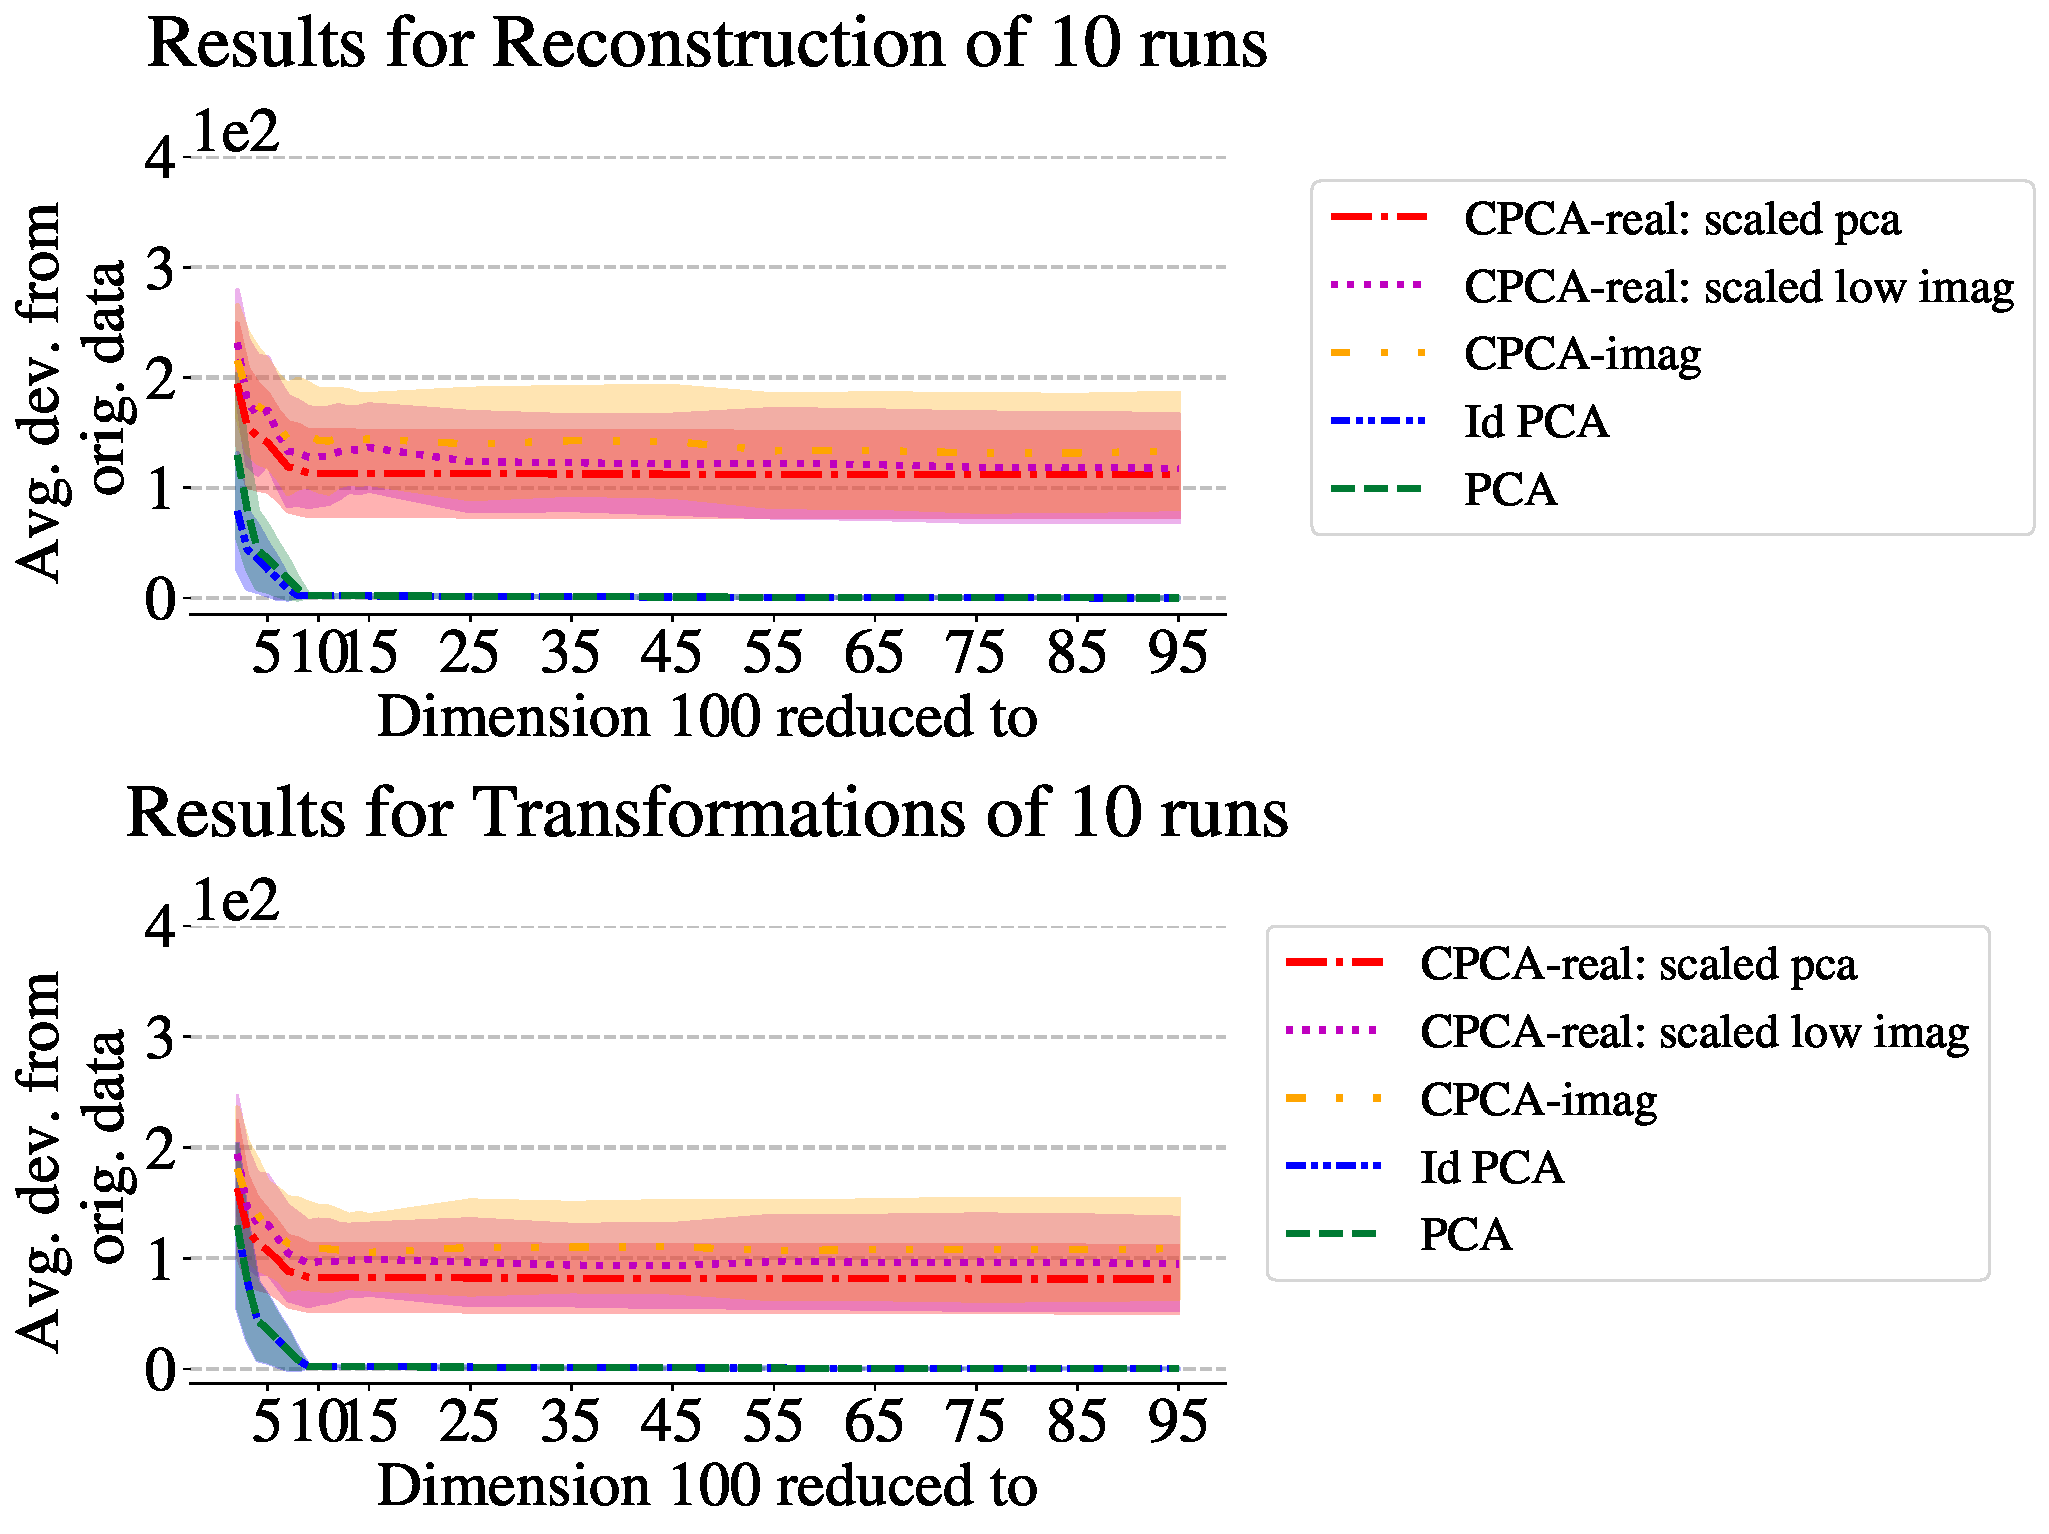
\includegraphics[width=7cm]{./images/multiple_runs/cpca/zigzag/avg_dev_vs_dyn_low/5lines_100points_1neighbours_euclidean.pdf}}
    \subfigure[Neighbour-Relation Measure]{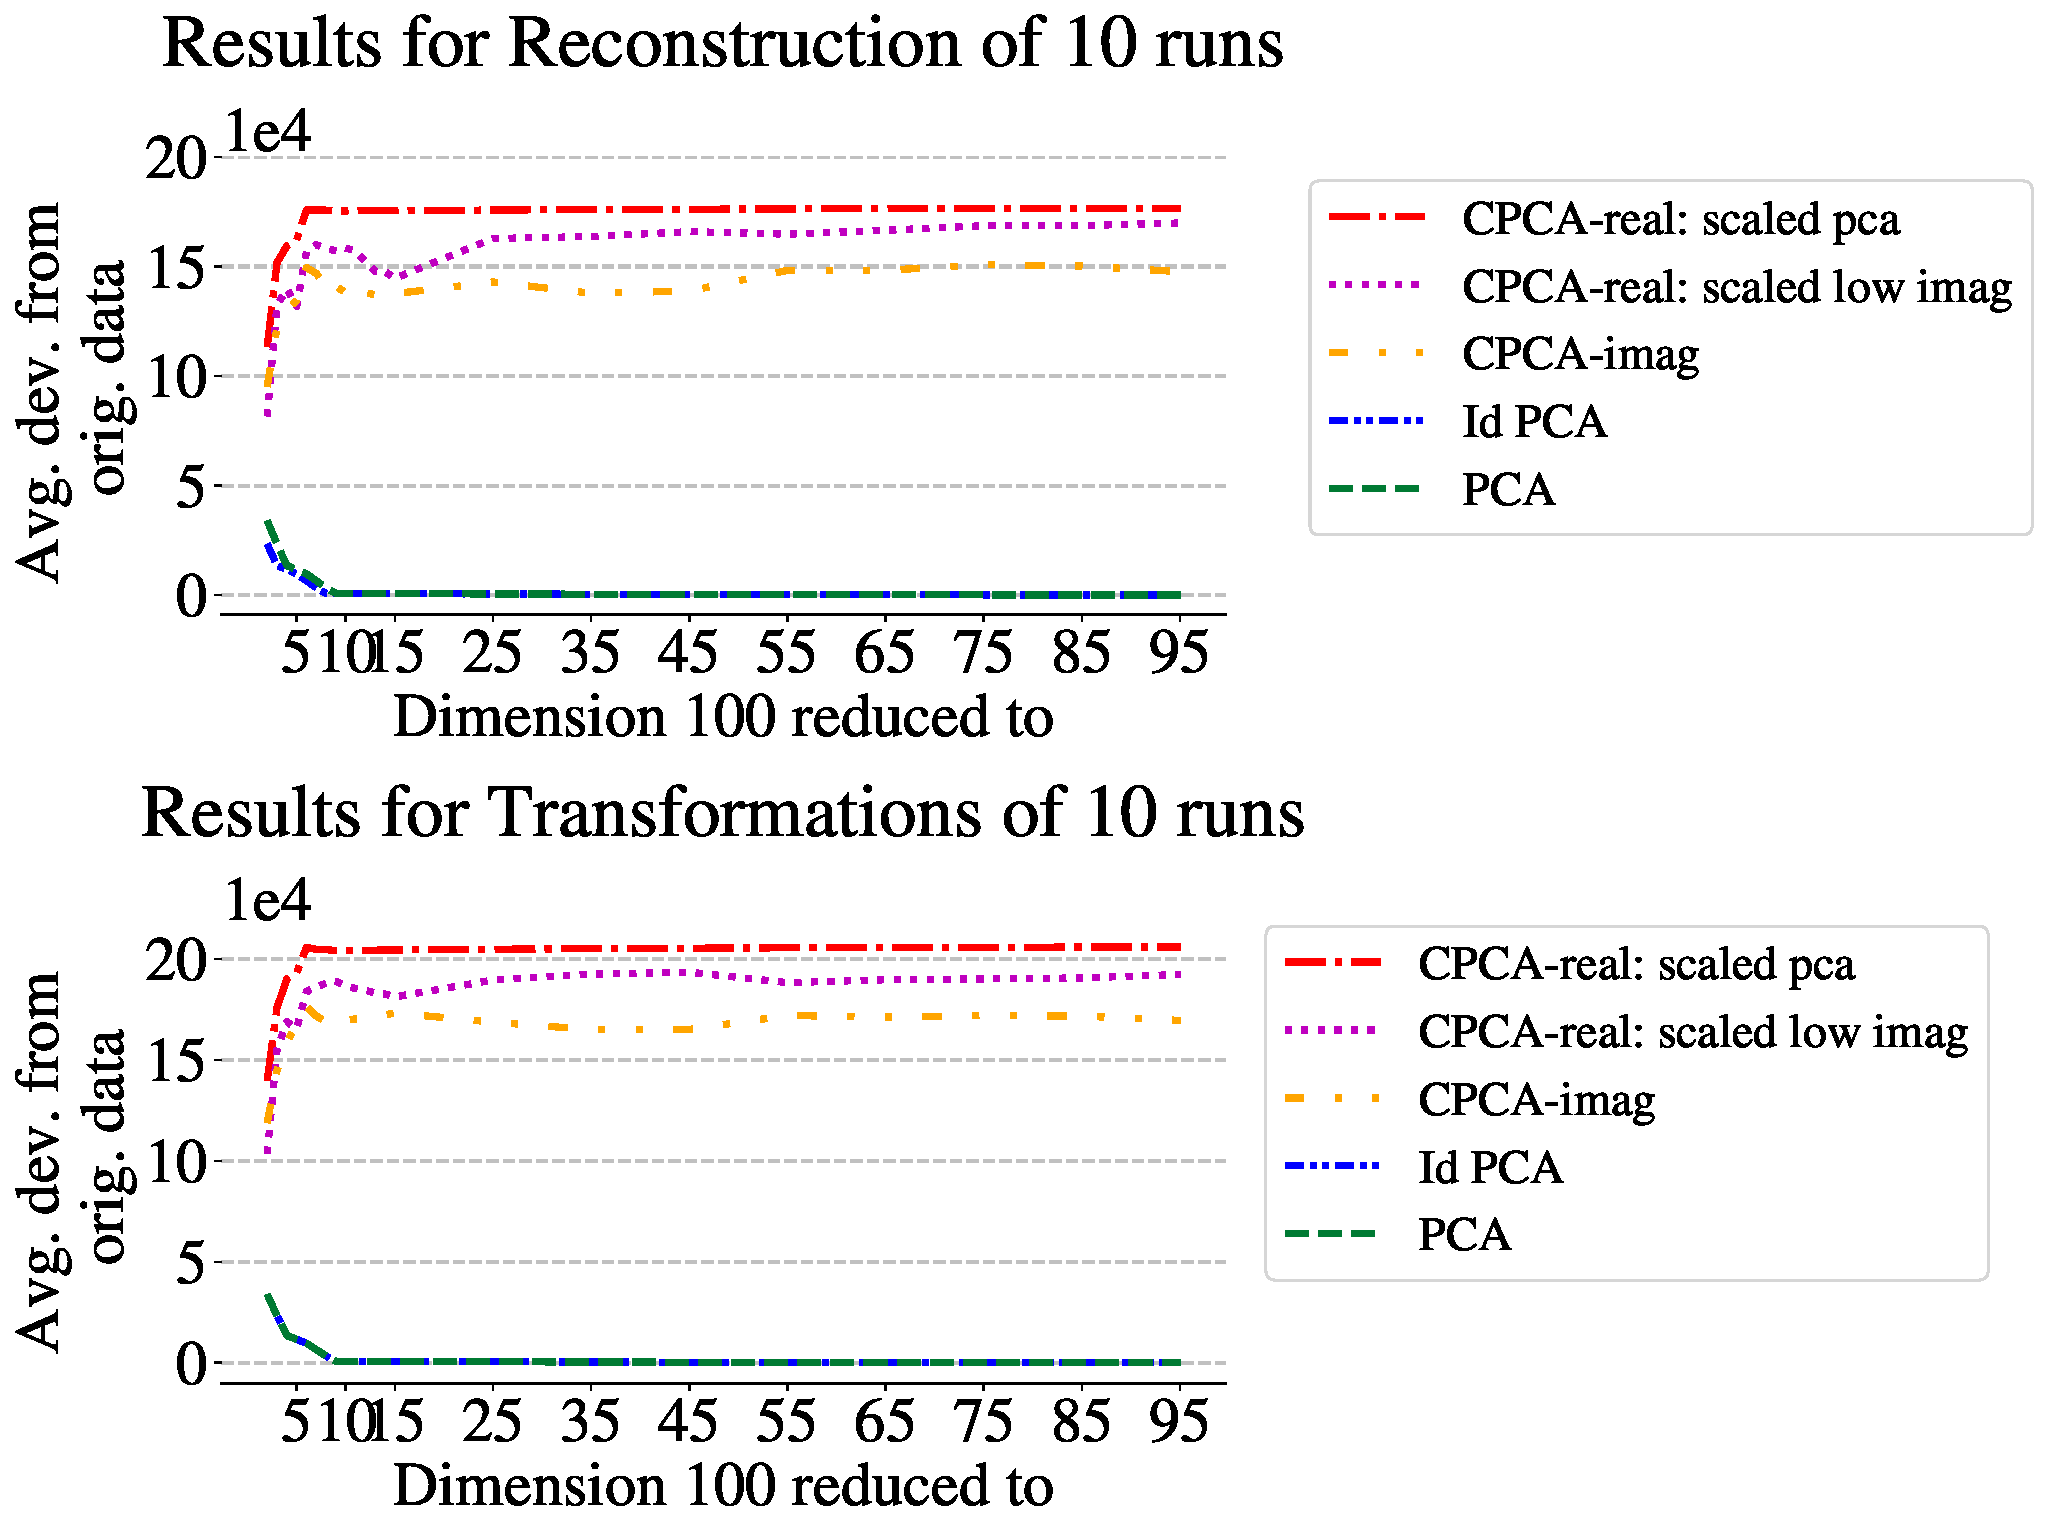
\includegraphics[width=7cm]{./images/multiple_runs/cpca/zigzag/avg_dev_vs_dyn_low/5lines_100points_1neighbours_multiple_scalar_product.pdf}}
    \caption{Results for zigzag data: comparing the summed distances between each predecessor and successor for data points in the original dataset and their reduced/reconstructed representations as dimensions increase}\label{fig:cpca-avg_dev_vs_high_dim-zigzag}
\end{figure}
Furthermore, we progressively increase the number of dimensions in each transformation.
This step allows us to explore the impact of dimensionality on the quality of order-based distance and relation preservation.


\begin{figure}
    \subfigure[Neighbour-Distance Measure]{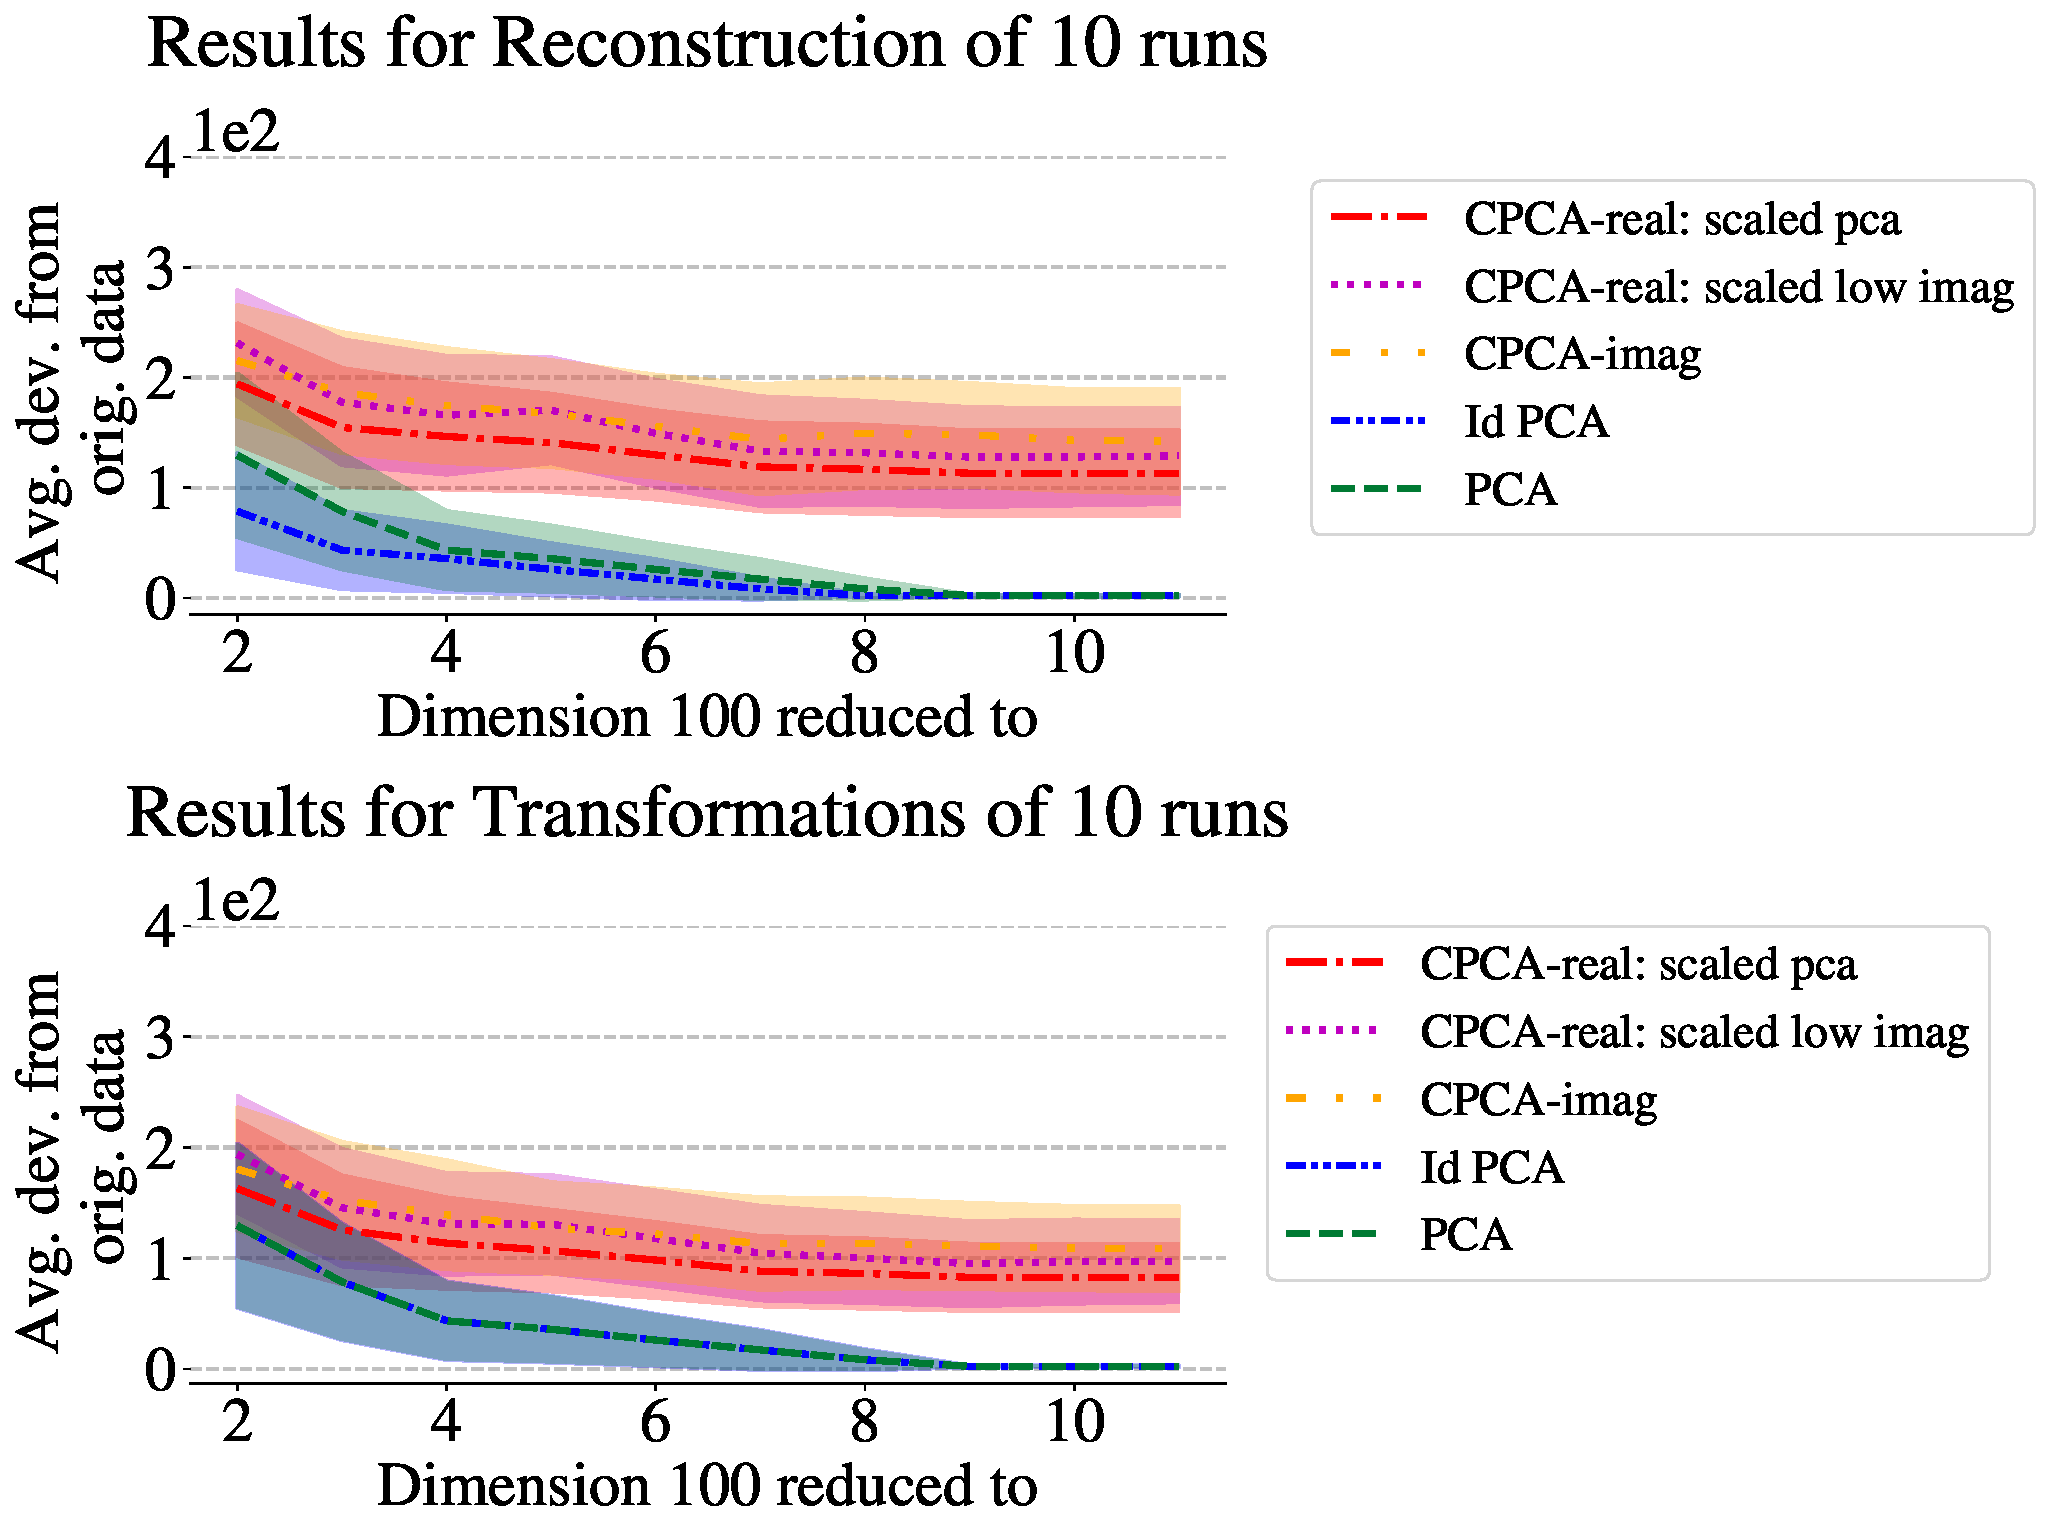
\includegraphics[width=7cm]{./images/multiple_runs/cpca/zigzag/avg_dev_vs_dyn_low/5lines_100points_1neighbours_euclidean_cutk10.pdf}}
    \subfigure[Neighbour-Relation Measure]{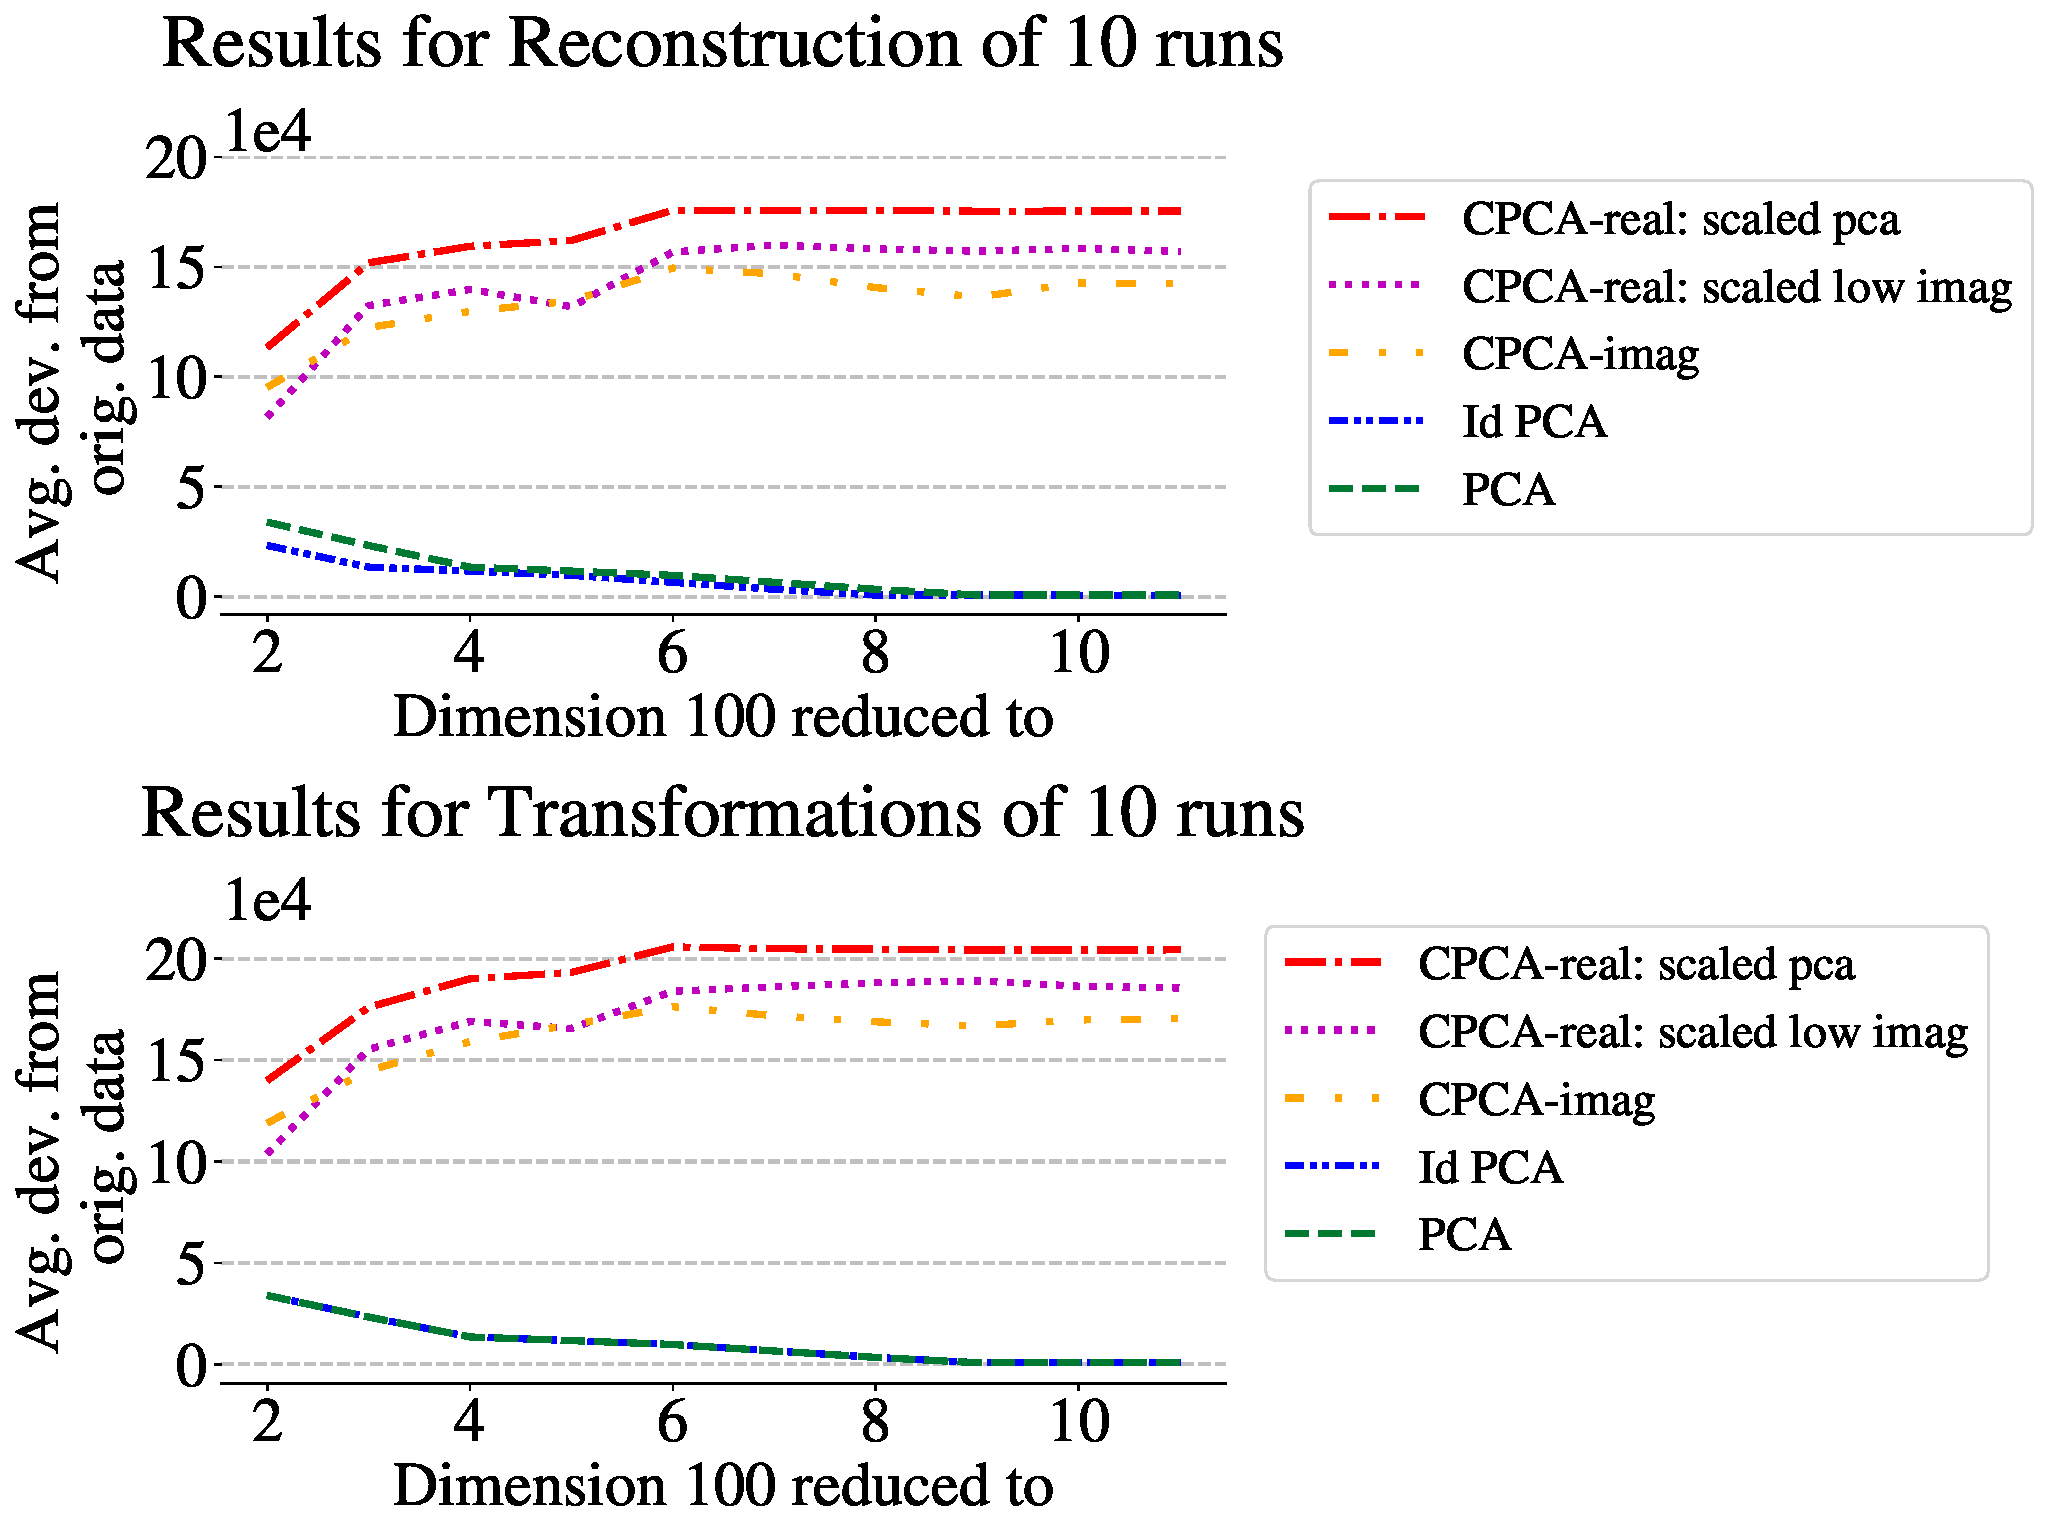
\includegraphics[width=7cm]{./images/multiple_runs/cpca/zigzag/avg_dev_vs_dyn_low/5lines_100points_1neighbours_multiple_scalar_product_cutk10.pdf}}
    \caption{Results for zigzag data for transformation dimensions between 2 and 10: comparing the summed distances between each predecessor and successor for data points in the original dataset and their reduced/reconstructed representations as dimensions increase} \label{fig:cpca-avg_dev_vs_high_dim-cut-zigzag}
\end{figure}

In this experiment setting, Figure~\ref{fig:cpca-avg_dev_vs_high_dim-zigzag} presents the results of PCA, Id PCA and the CPCA variants applied to zigzag data.
The outcomes for all three CPCA variants show poor performance in both the reconstructed and transformed representations, assessed with both measures. 
However, Id PCA exhibits a similar outcome to PCA while better preserving the cumulative distances to each predecessor and successor of every data point, as measured by the ND metric.
This is also shown in Figure~\ref{fig:cpca-avg_dev_vs_high_dim-cut-zigzag}, which focuses on dimensions between 2 and 10, a range often preferred for analysis.

\begin{figure}[htb!]
    \subfigure[Neighbour-Distance Measure]{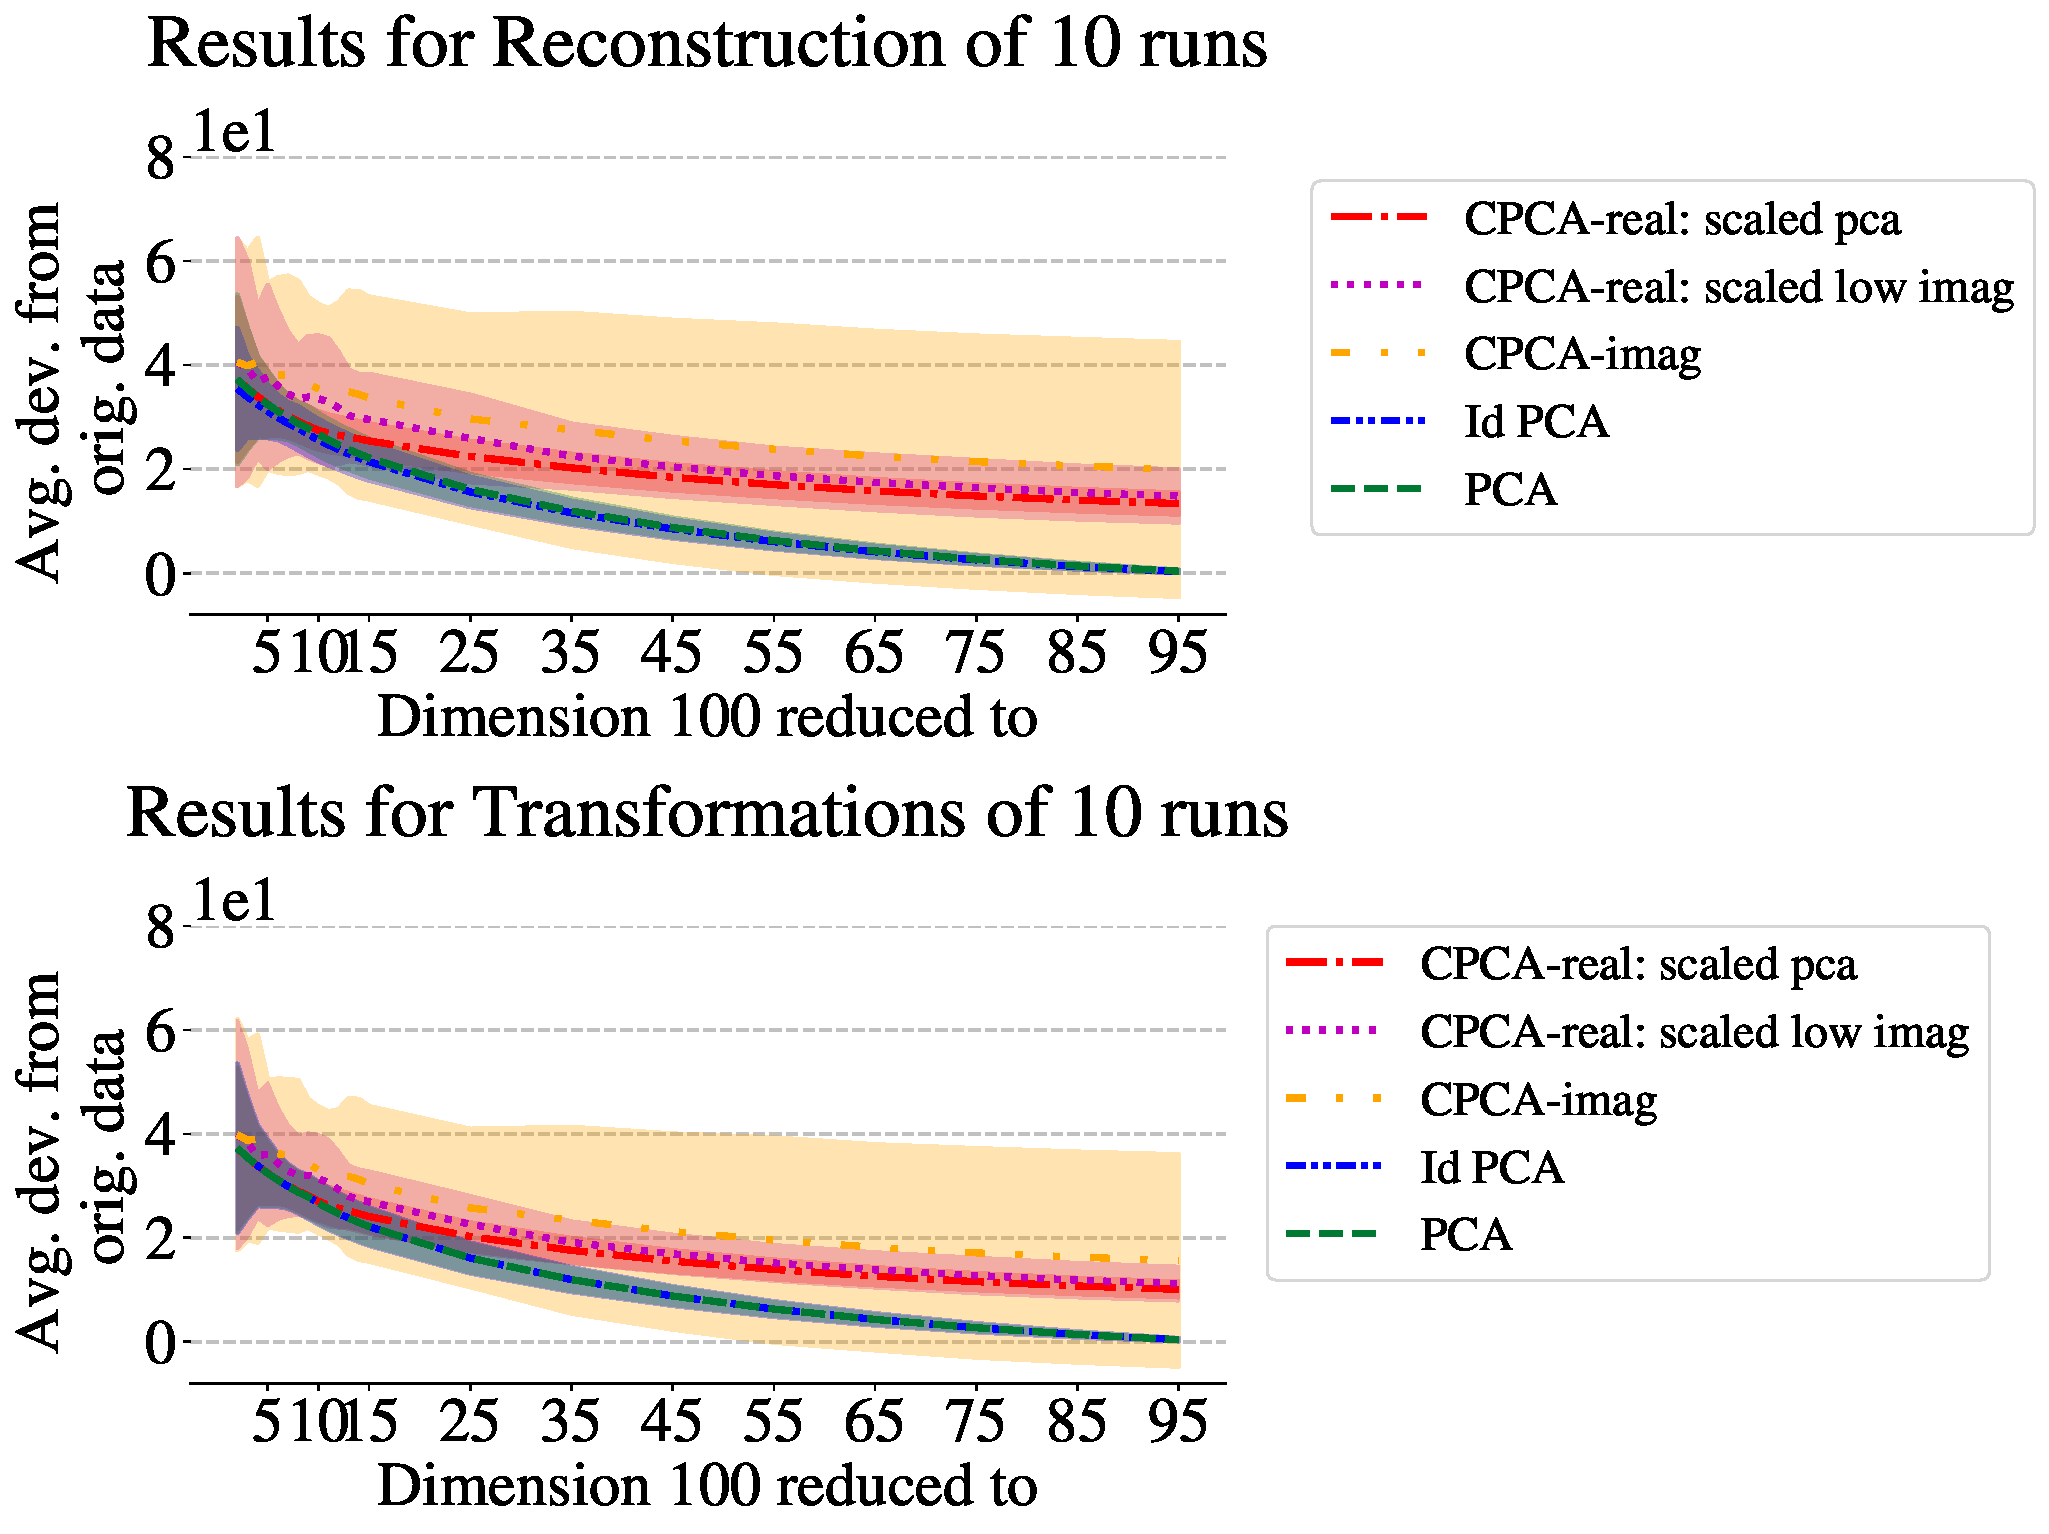
\includegraphics[width=7cm]{./images/multiple_runs/cpca/one_line/avg_dev_vs_dyn_low/5lines_100points_1neighbours_euclidean.pdf}}
    \subfigure[Neighbour-Relation Measure]{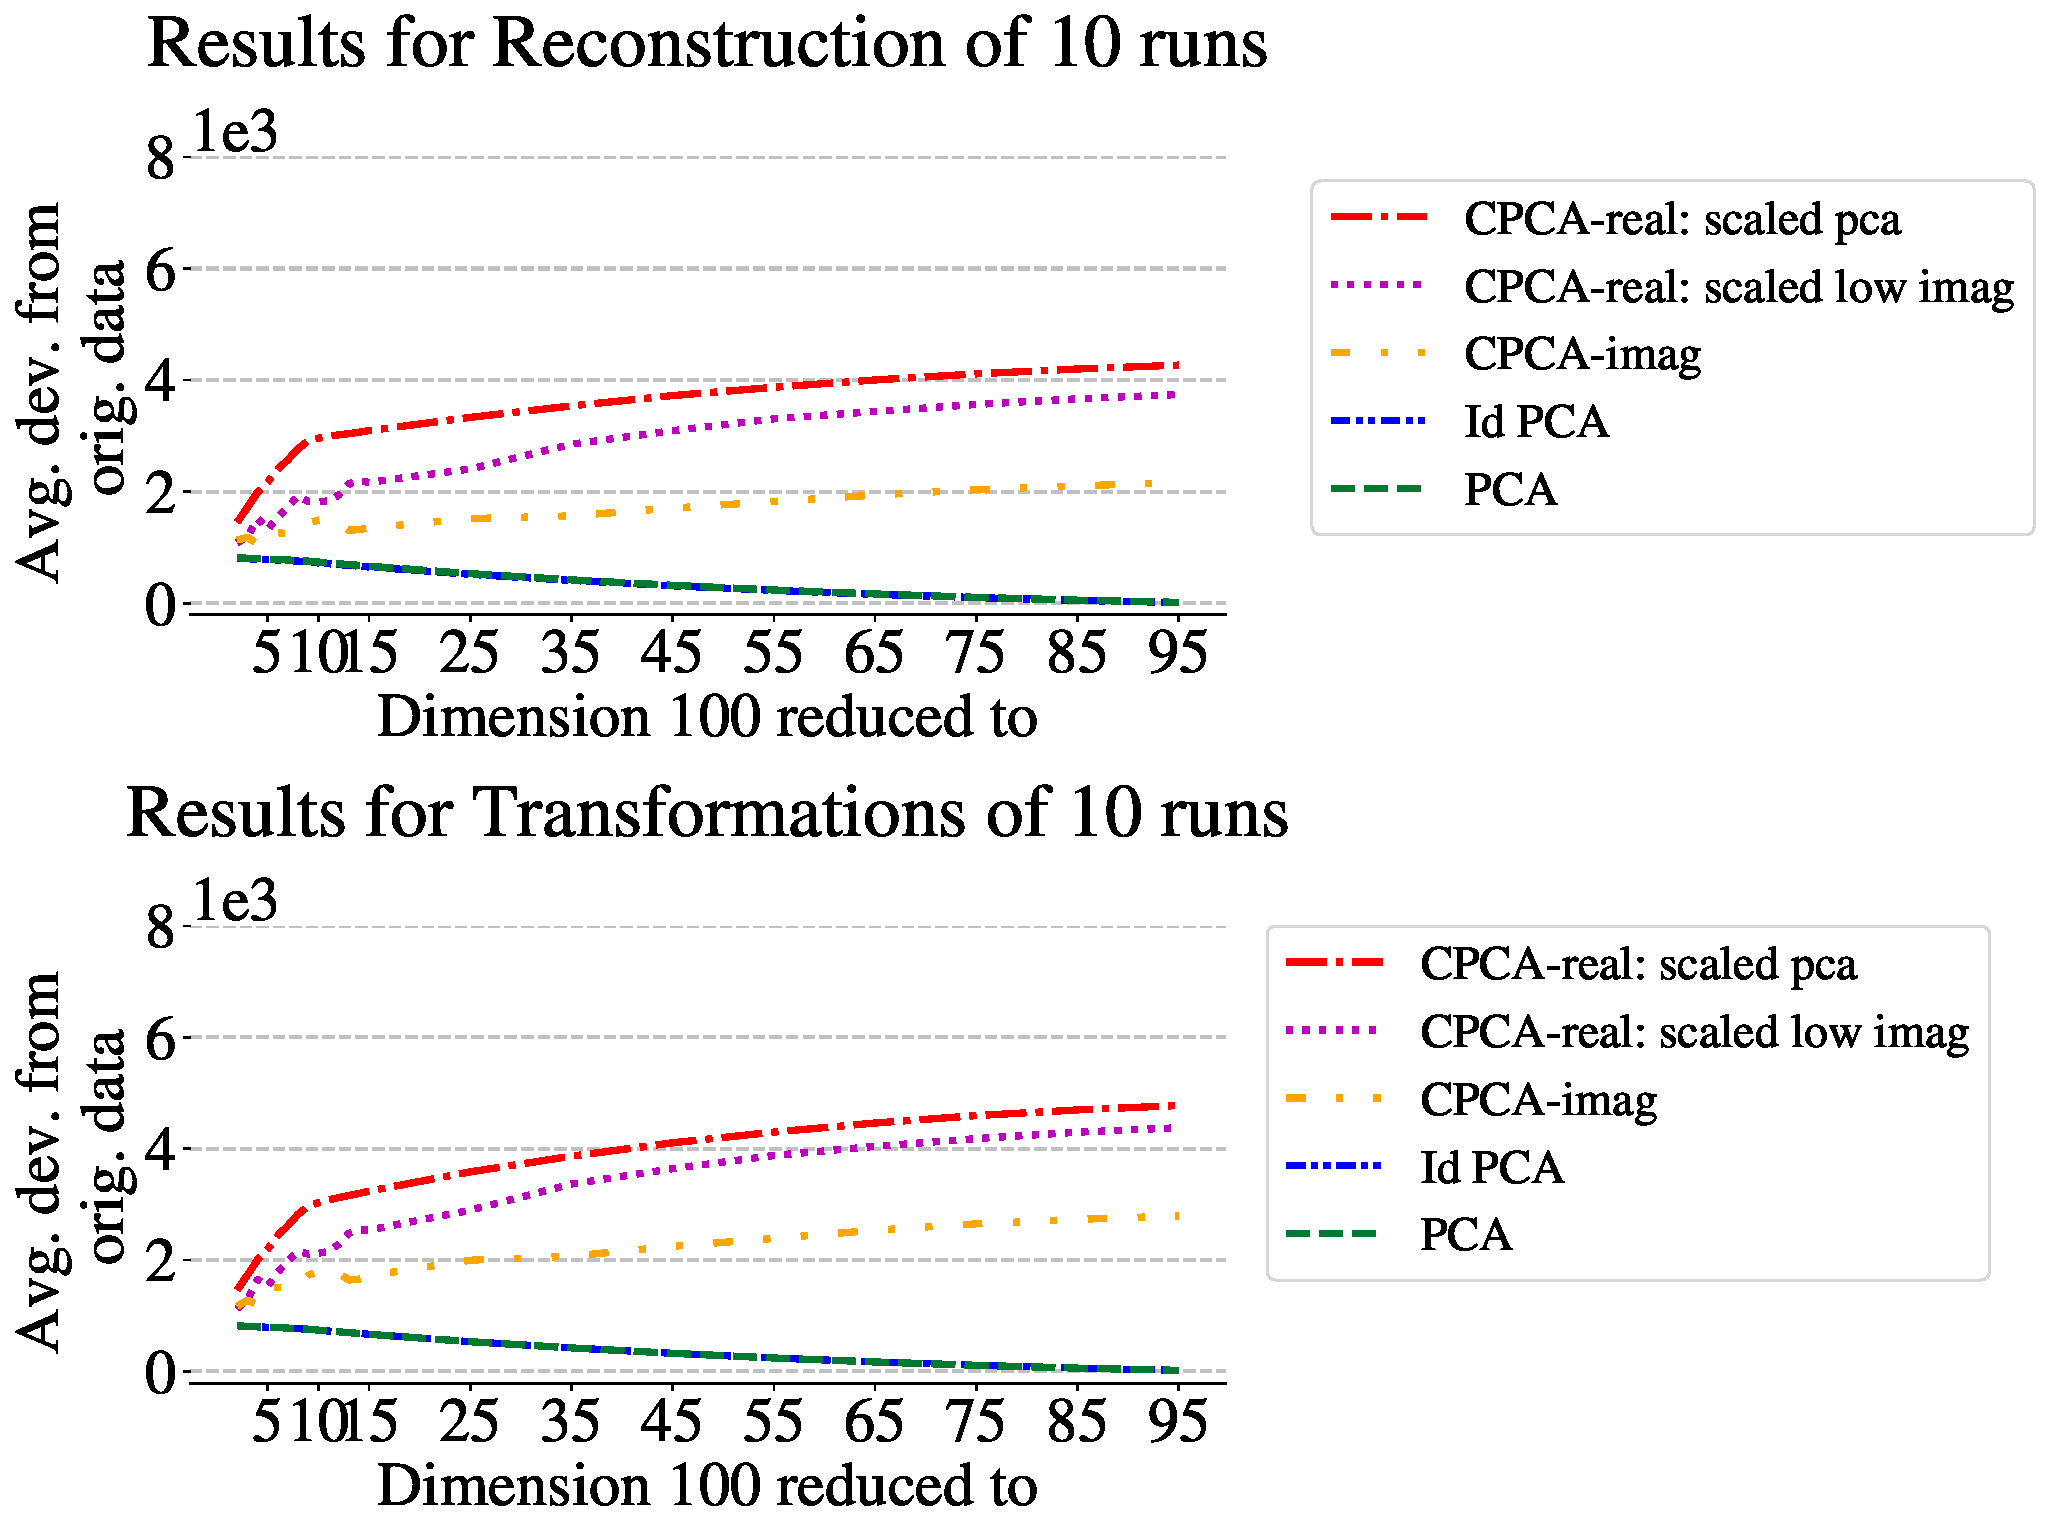
\includegraphics[width=7cm]{./images/multiple_runs/cpca/one_line/avg_dev_vs_dyn_low/5lines_100points_1neighbours_multiple_scalar_product.pdf}}
    \caption{Results for smoothly ordered data: comparing the summed distances between each predecessor and successor for data points in the original dataset and their reduced/reconstructed representations as dimensions increase}\label{fig:cpca-avg_dev_vs_high_dim-oneline}
\end{figure}
\begin{figure}[htb!]
    \subfigure[Neighbour-Distance Measure]{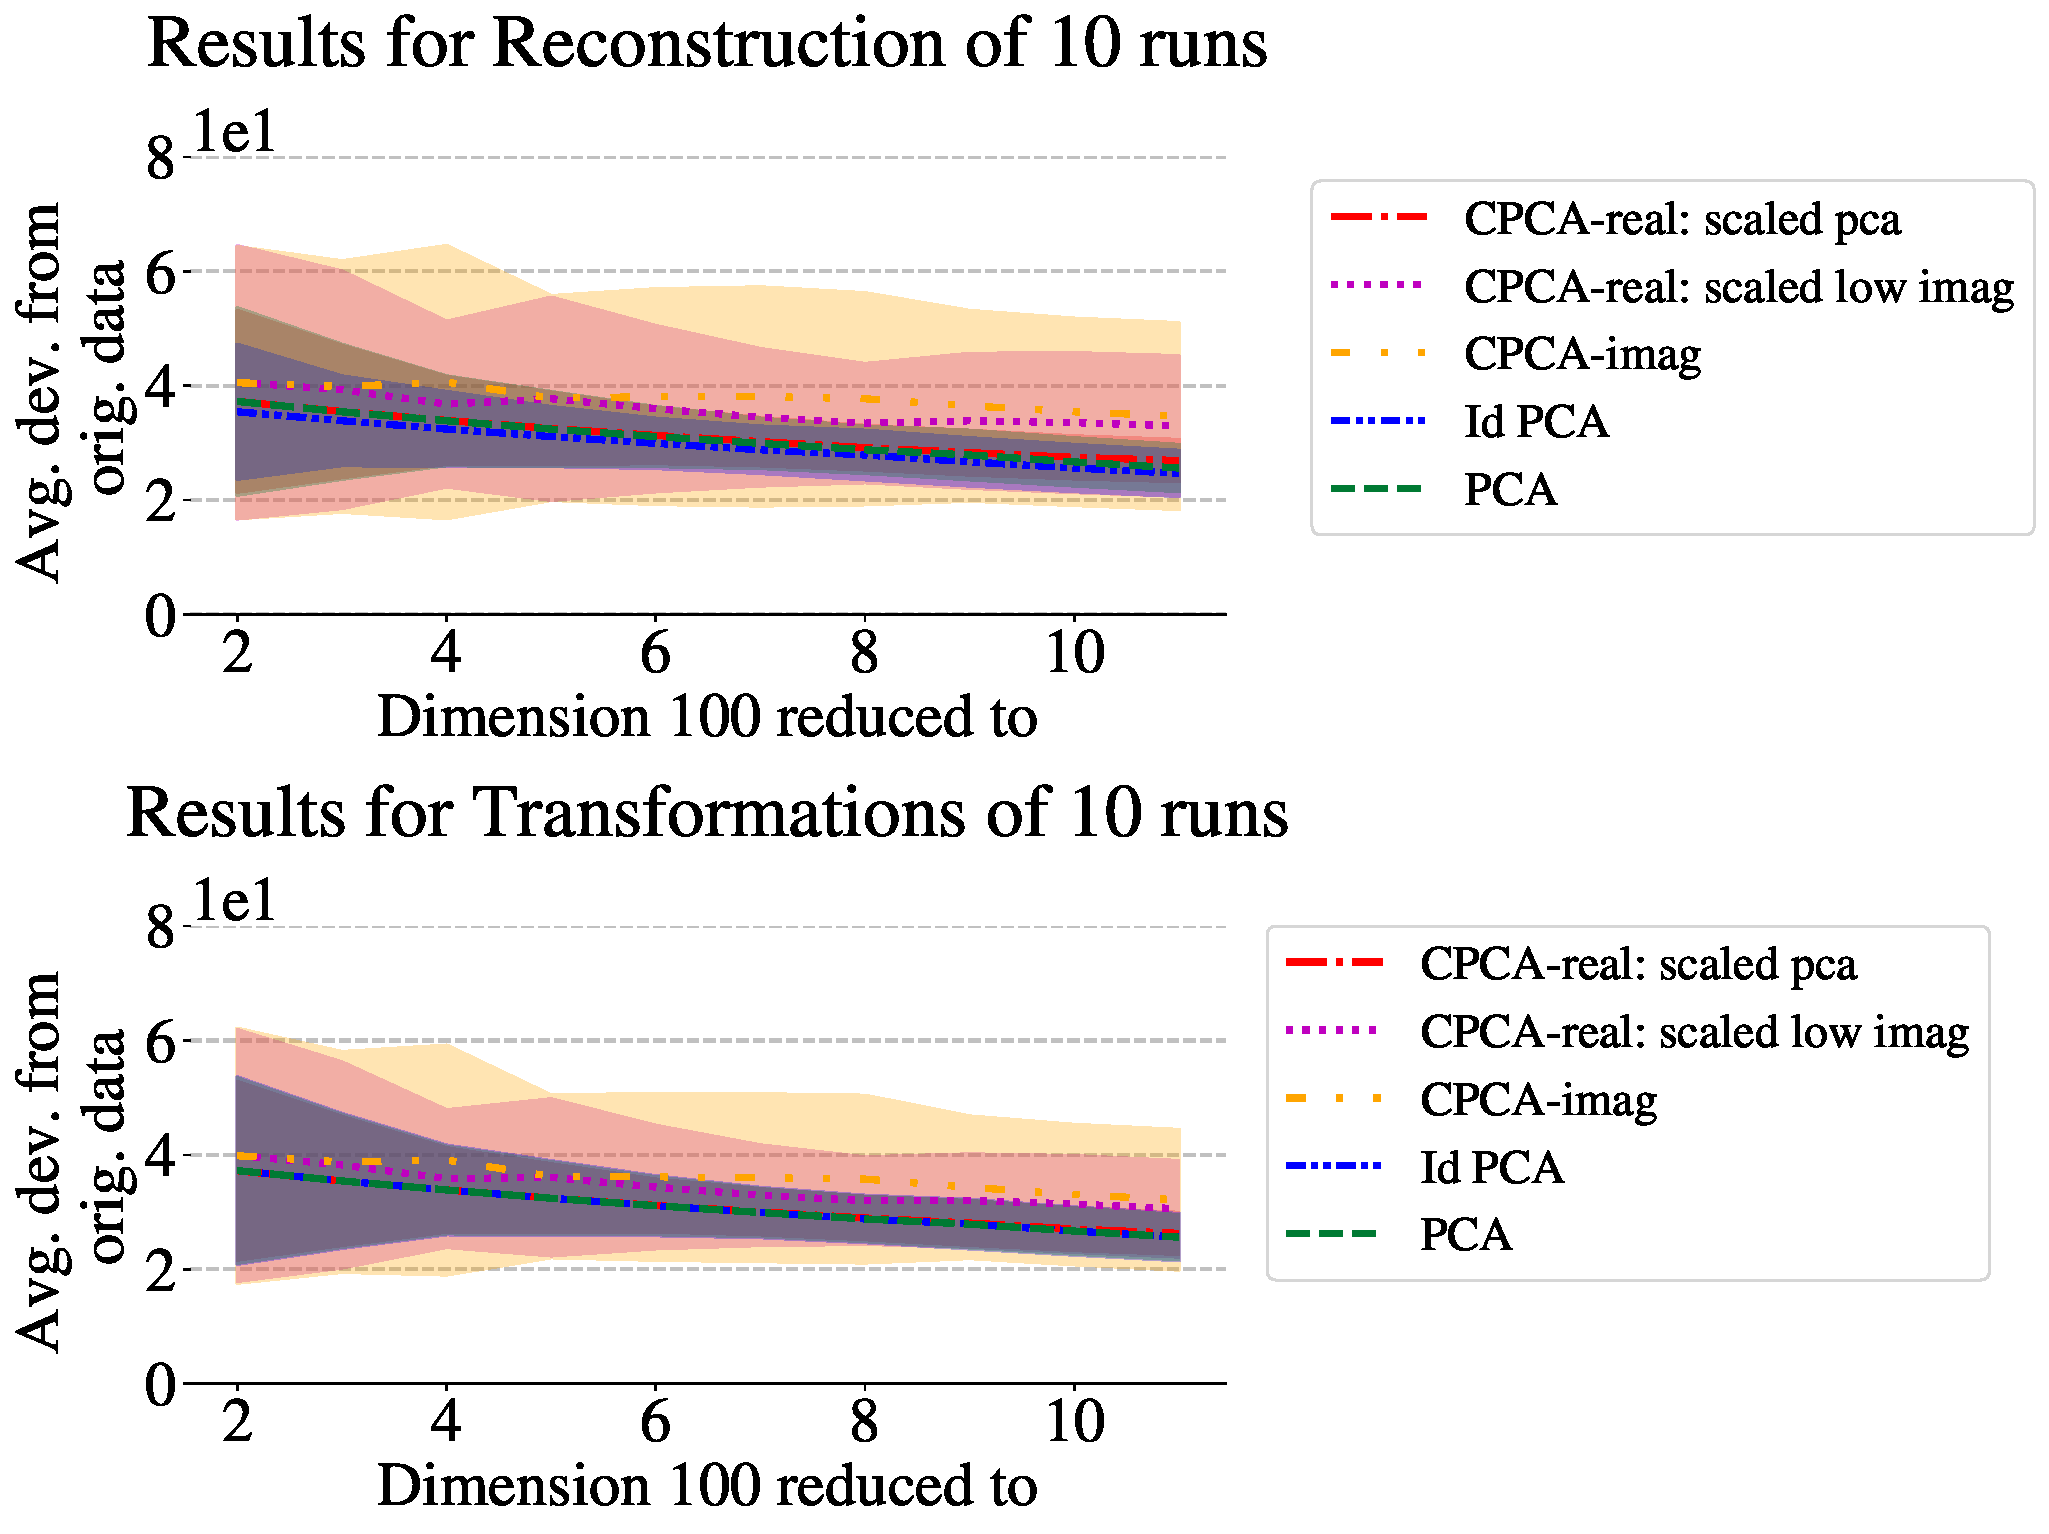
\includegraphics[width=7cm]{./images/multiple_runs/cpca/one_line/avg_dev_vs_dyn_low/5lines_100points_1neighbours_euclidean_cutk10.pdf}}
    \subfigure[Neighbour-Relation Measure]{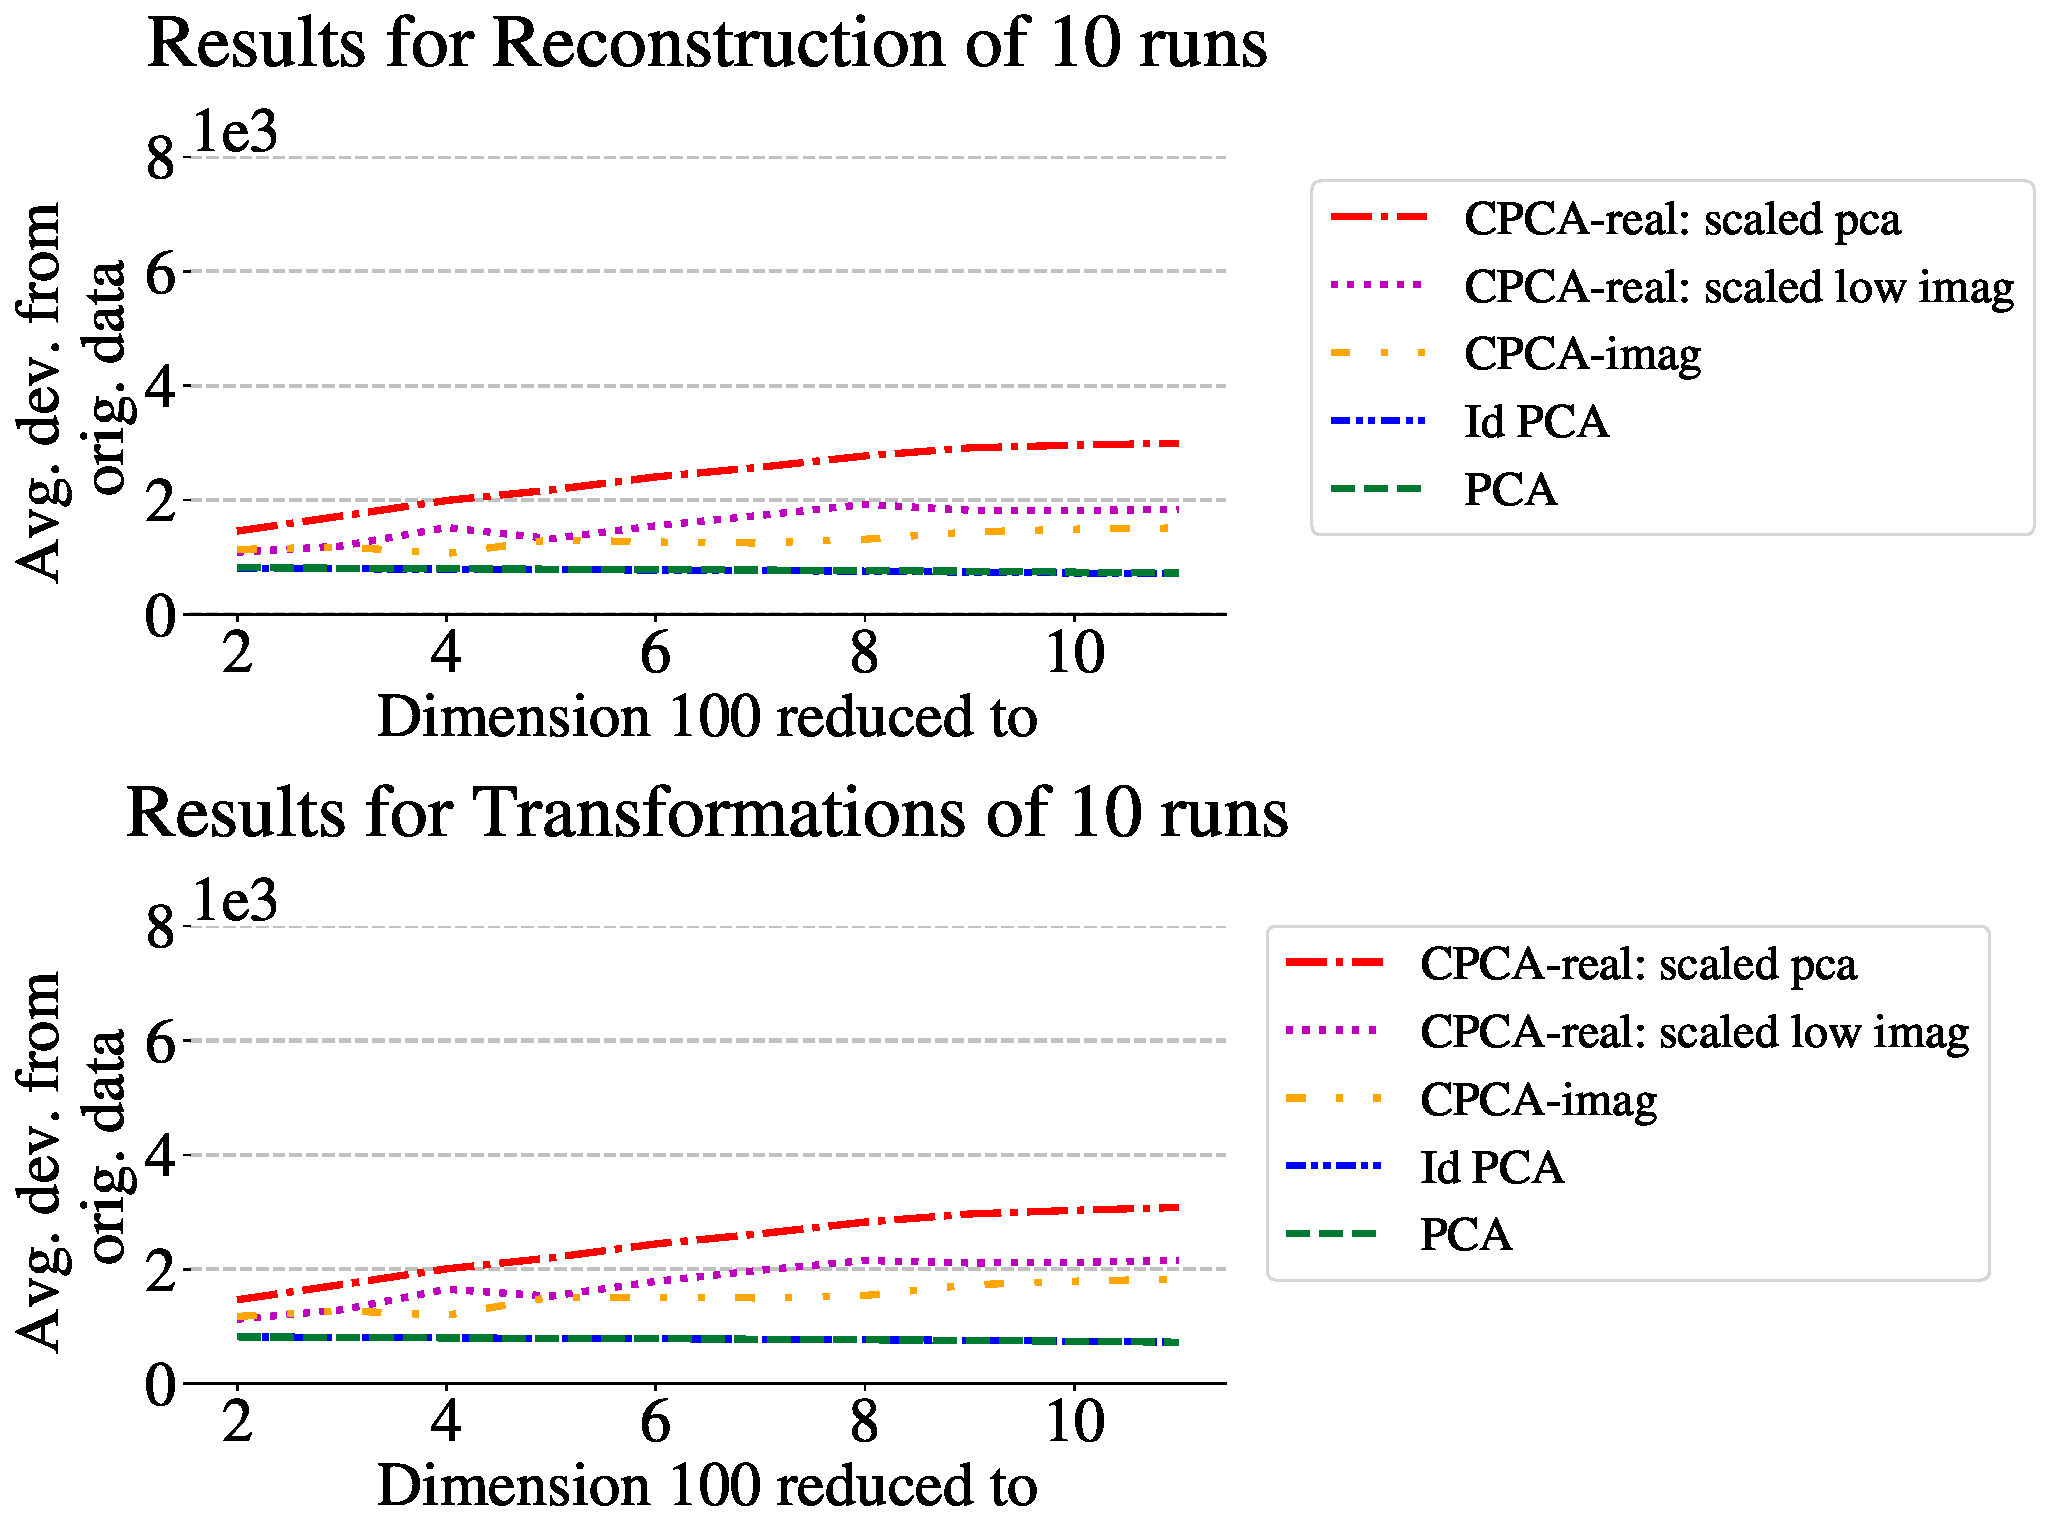
\includegraphics[width=7cm]{./images/multiple_runs/cpca/one_line/avg_dev_vs_dyn_low/5lines_100points_1neighbours_multiple_scalar_product_cutk10.pdf}}
    \caption{Results for smoothly ordered data for transformation dimensions between 2 and 10: comparing the summed distances between each predecessor and successor for data points in the original dataset and their reduced/reconstructed representations as dimensions increase}\label{fig:cpca-avg_dev_vs_high_dim-cut-oneline}
\end{figure}
% In Figure \ref{fig:cpca-avg_dev_vs_high_dim-oneline}, we observe similar mean values of the 10 runs for all three CPCA variants applied to smoothly ordered data.
% However, CPCA-imag exhibits high variance when we measure the euclidean distances between the first neighbours of each data point.
% However, CPCA-imag maintains order-based relations better than the other two variants.
% Overall maintain PCA and Id PCA similarly well distances and relations.

Applying the dimensionality reduction methods to data that is smoothly ordered gives similar results to them applied to zigzag data, see Figure~\ref{fig:cpca-avg_dev_vs_high_dim-oneline}.
Here the size of the variance of \textit{CPCA-imag} strikes as it is multiple times bigger than the variances of the results of the other dimensionality reduction methods measured with the ND measure.
Id PCA and PCA perform similarly well, with Id PCA maintaining the ND distances better for a lower number of dimensions but keeping the intra-point relations marginally worse in its reconstructed representation, see Figure~\ref{fig:cpca-avg_dev_vs_high_dim-cut-oneline}.

\begin{figure}[htb!]
    \subfigure[Neighbour-Distance Measure]{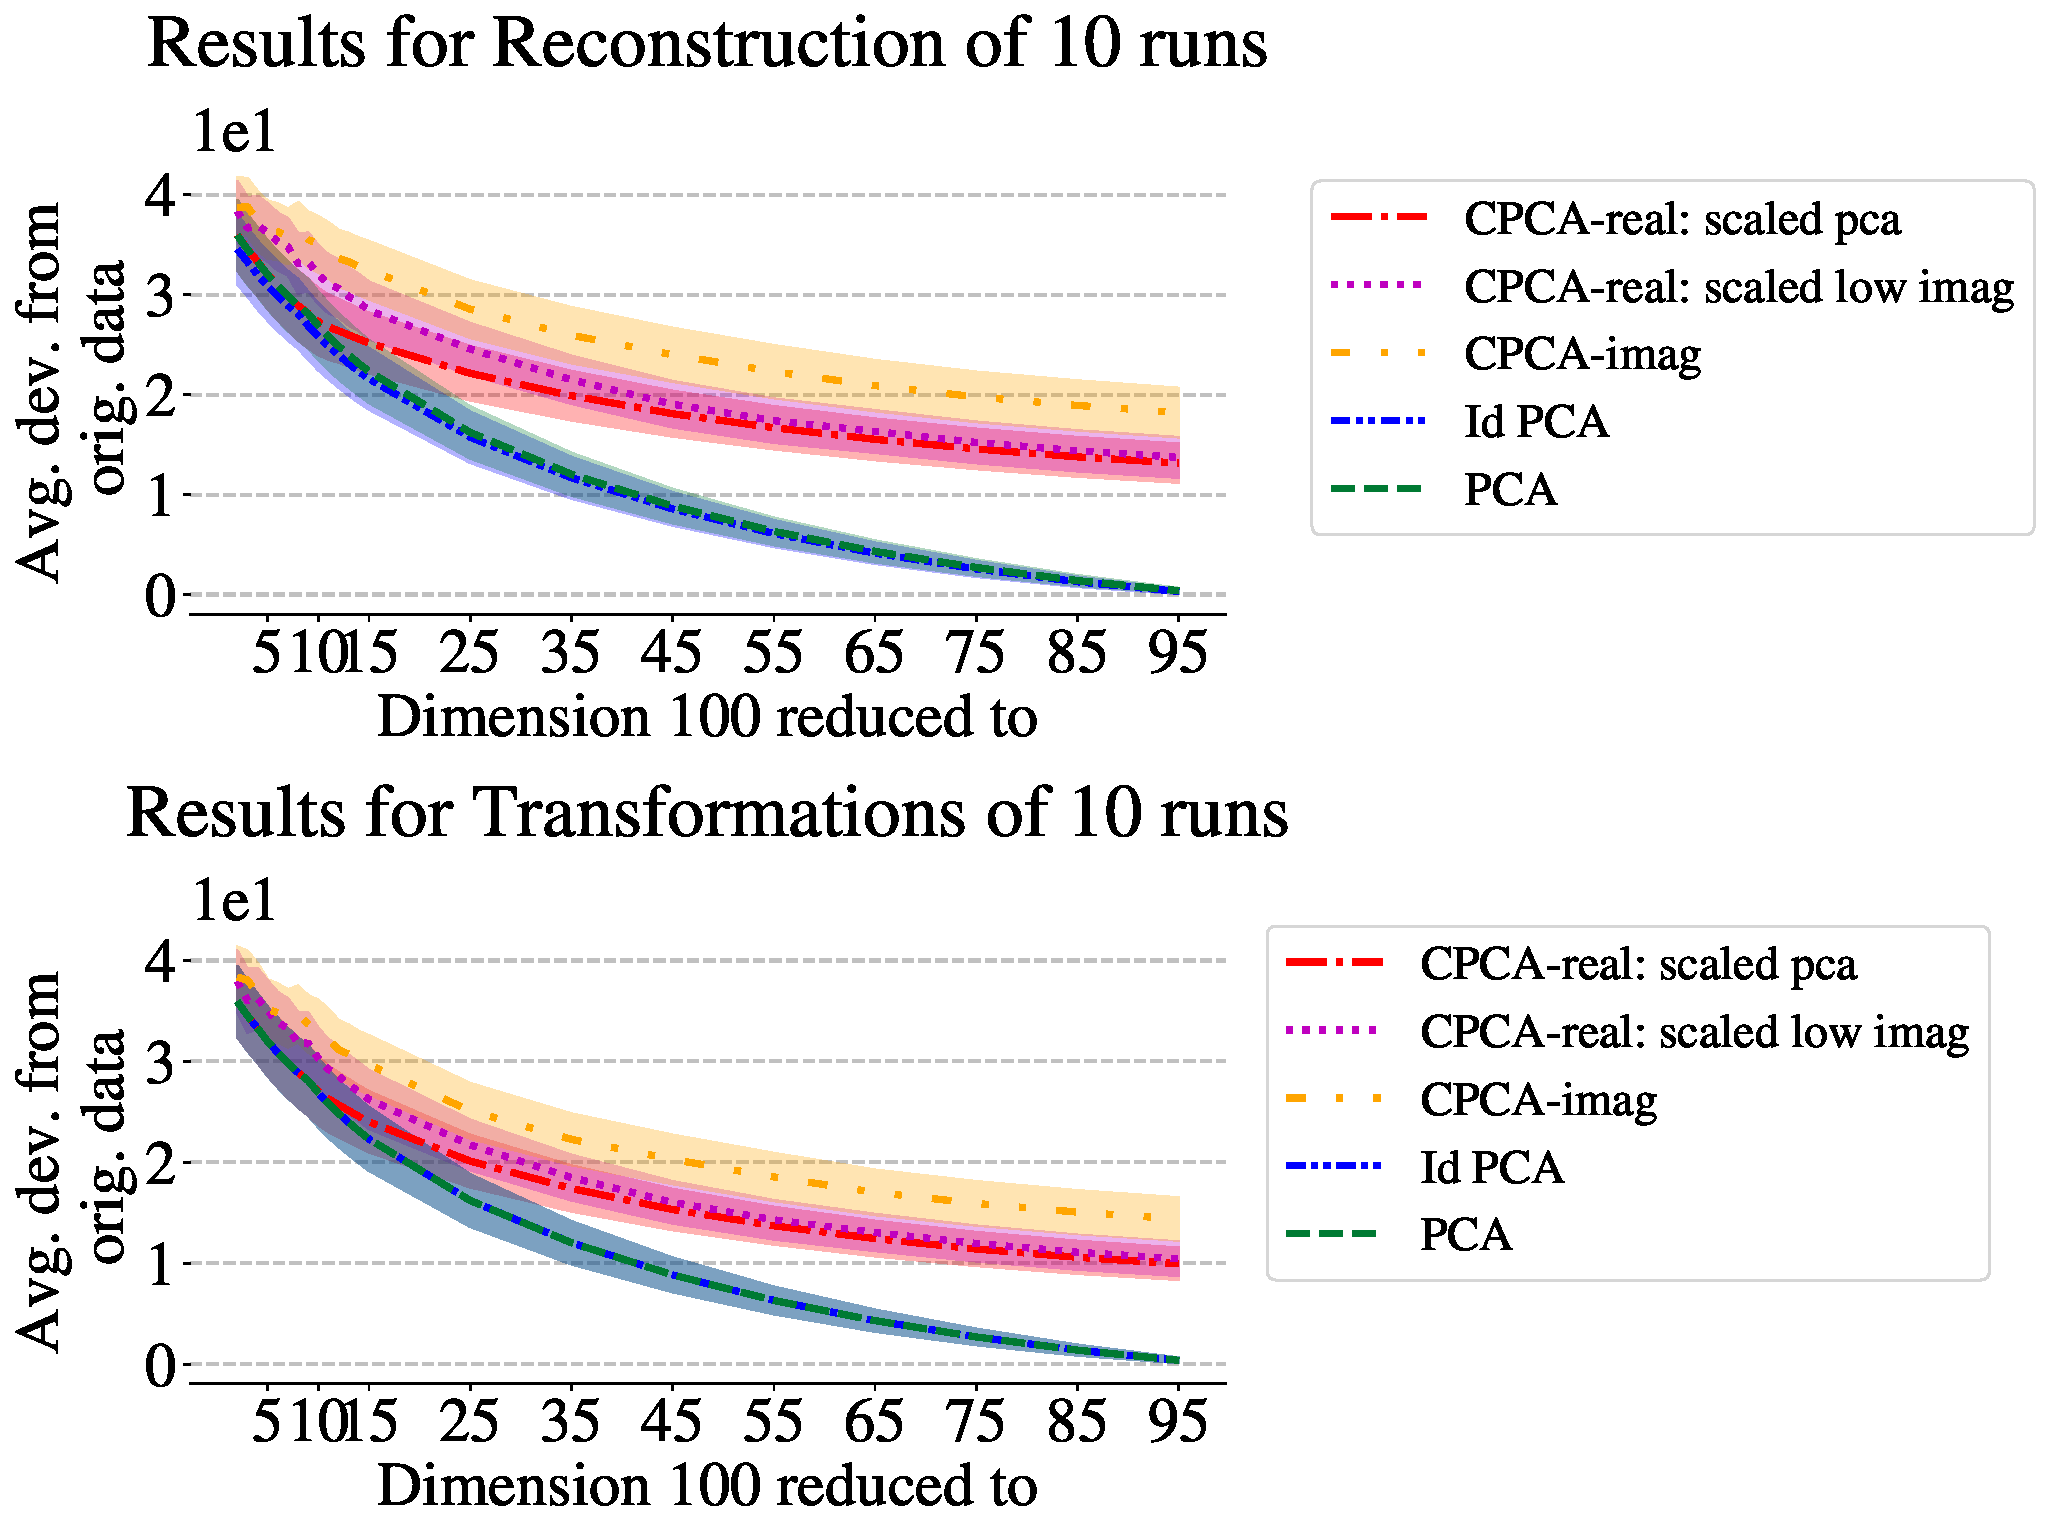
\includegraphics[width=7cm]{./images/multiple_runs/cpca/sep_lines/avg_dev_vs_dyn_low/5lines_100points_1neighbours_euclidean.pdf}}
    \subfigure[Neighbour-Relation Measure]{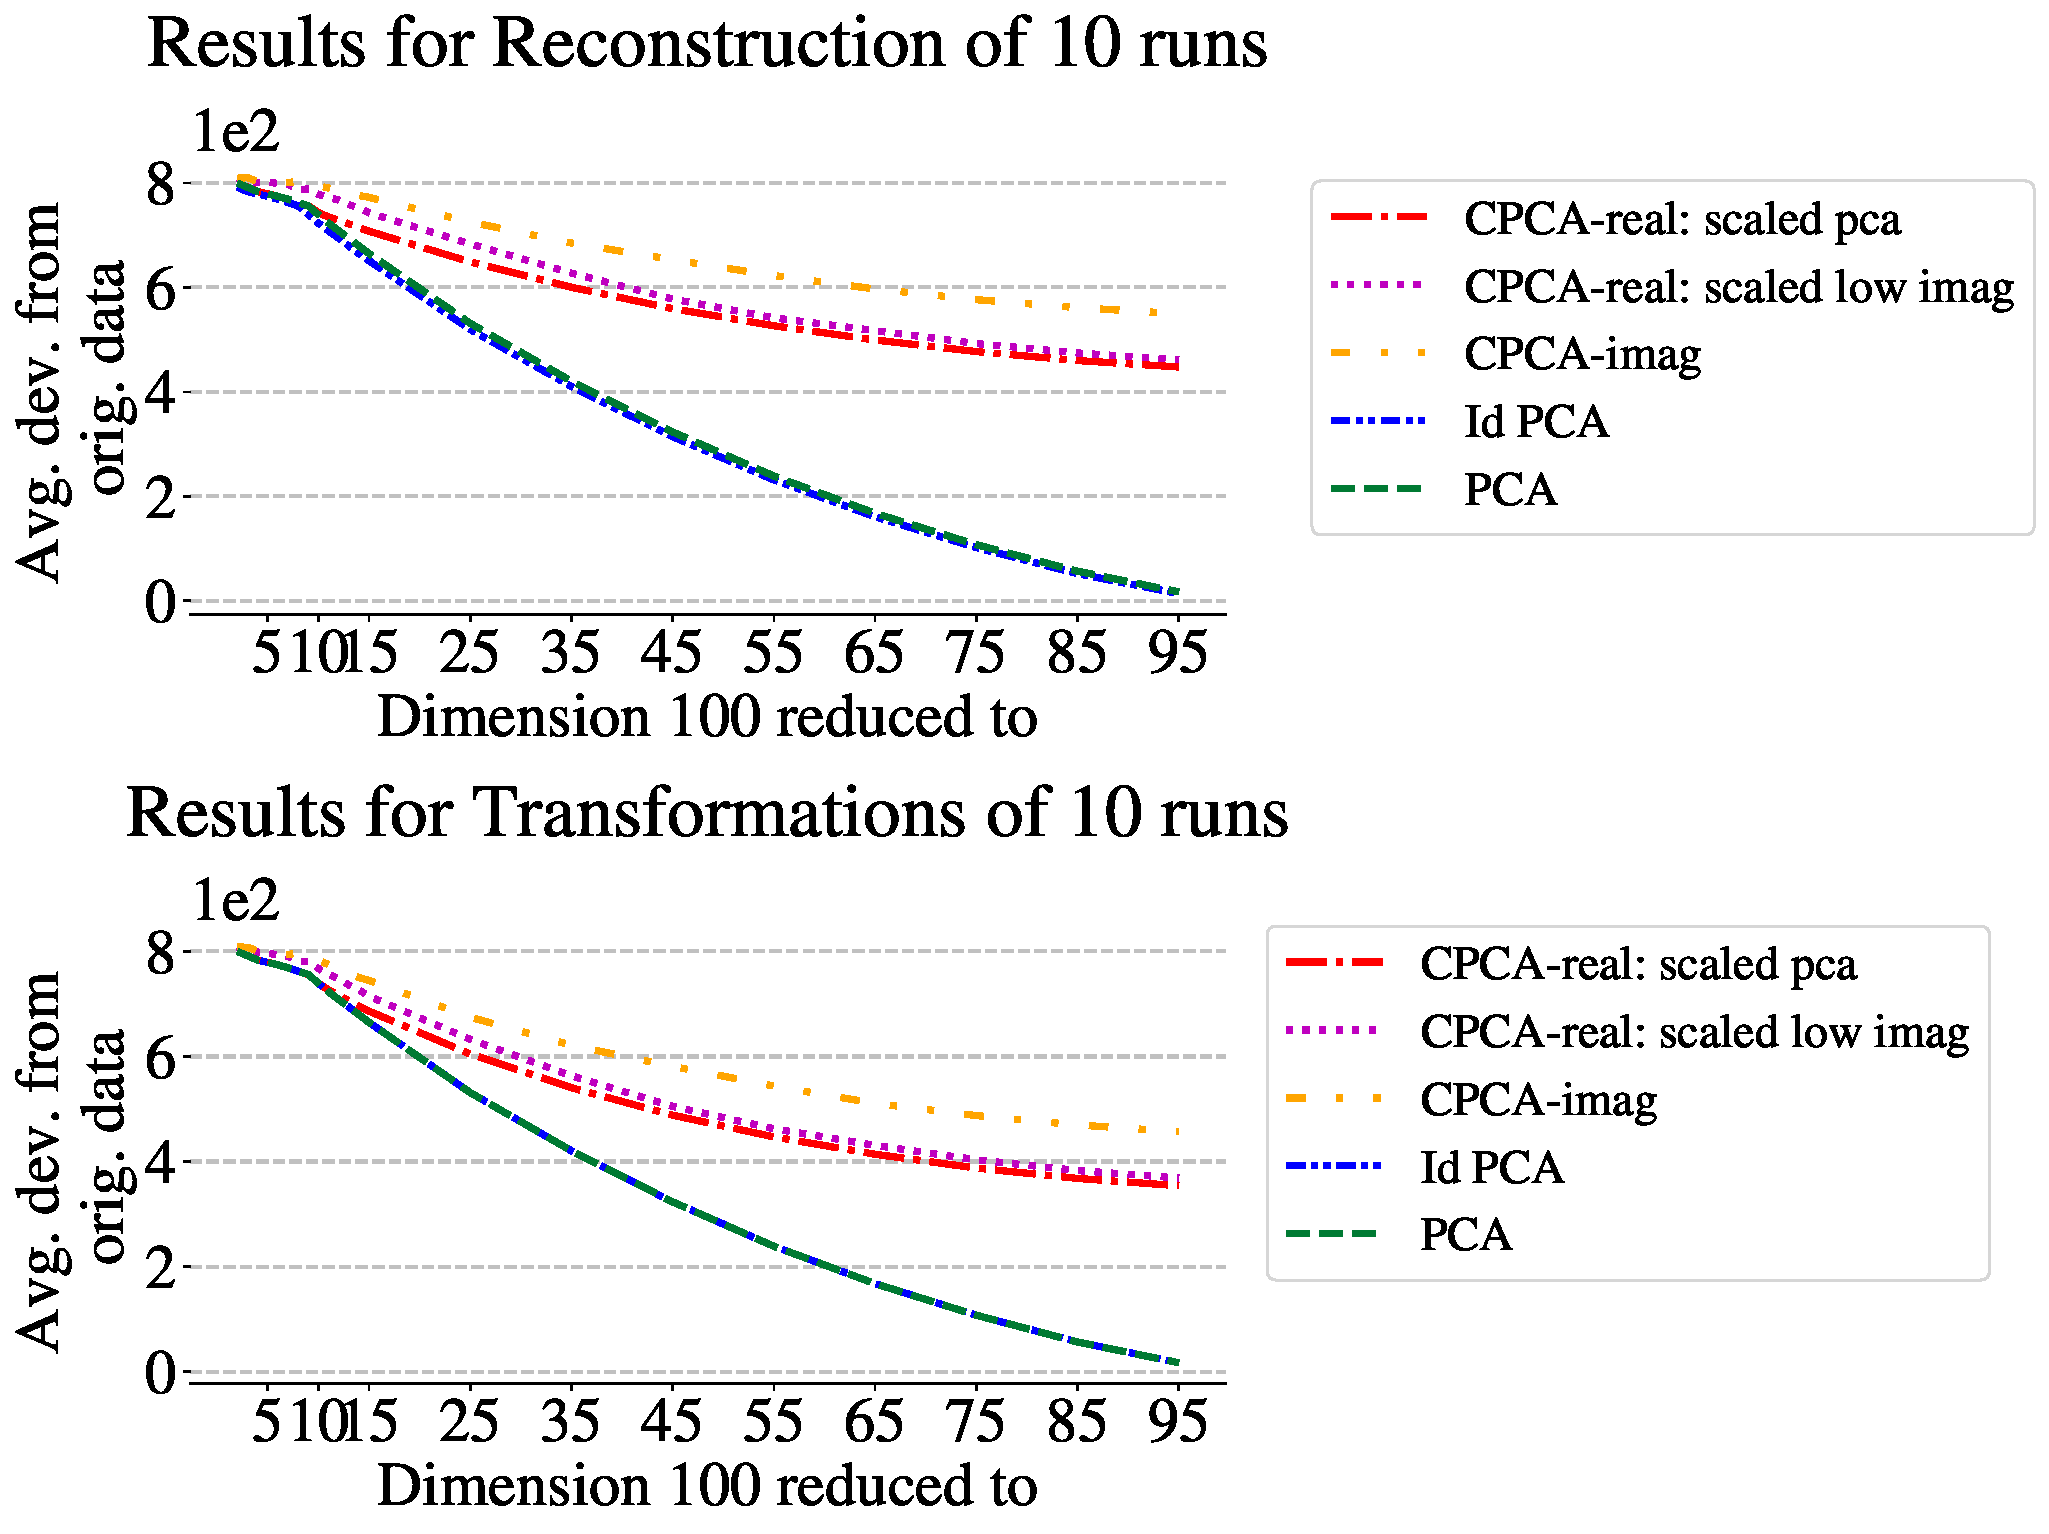
\includegraphics[width=7cm]{./images/multiple_runs/cpca/sep_lines/avg_dev_vs_dyn_low/5lines_100points_1neighbours_multiple_scalar_product.pdf}}
    \caption{Results for data in separate lines: comparing the summed distances between each predecessor and successor for data points in the original dataset and their reduced/reconstructed representations as dimensions increase}\label{fig:cpca-avg_dev_vs_high_dim-seplines}
\end{figure}

\begin{figure}
    \subfigure[Neighbour-Distance Measure]{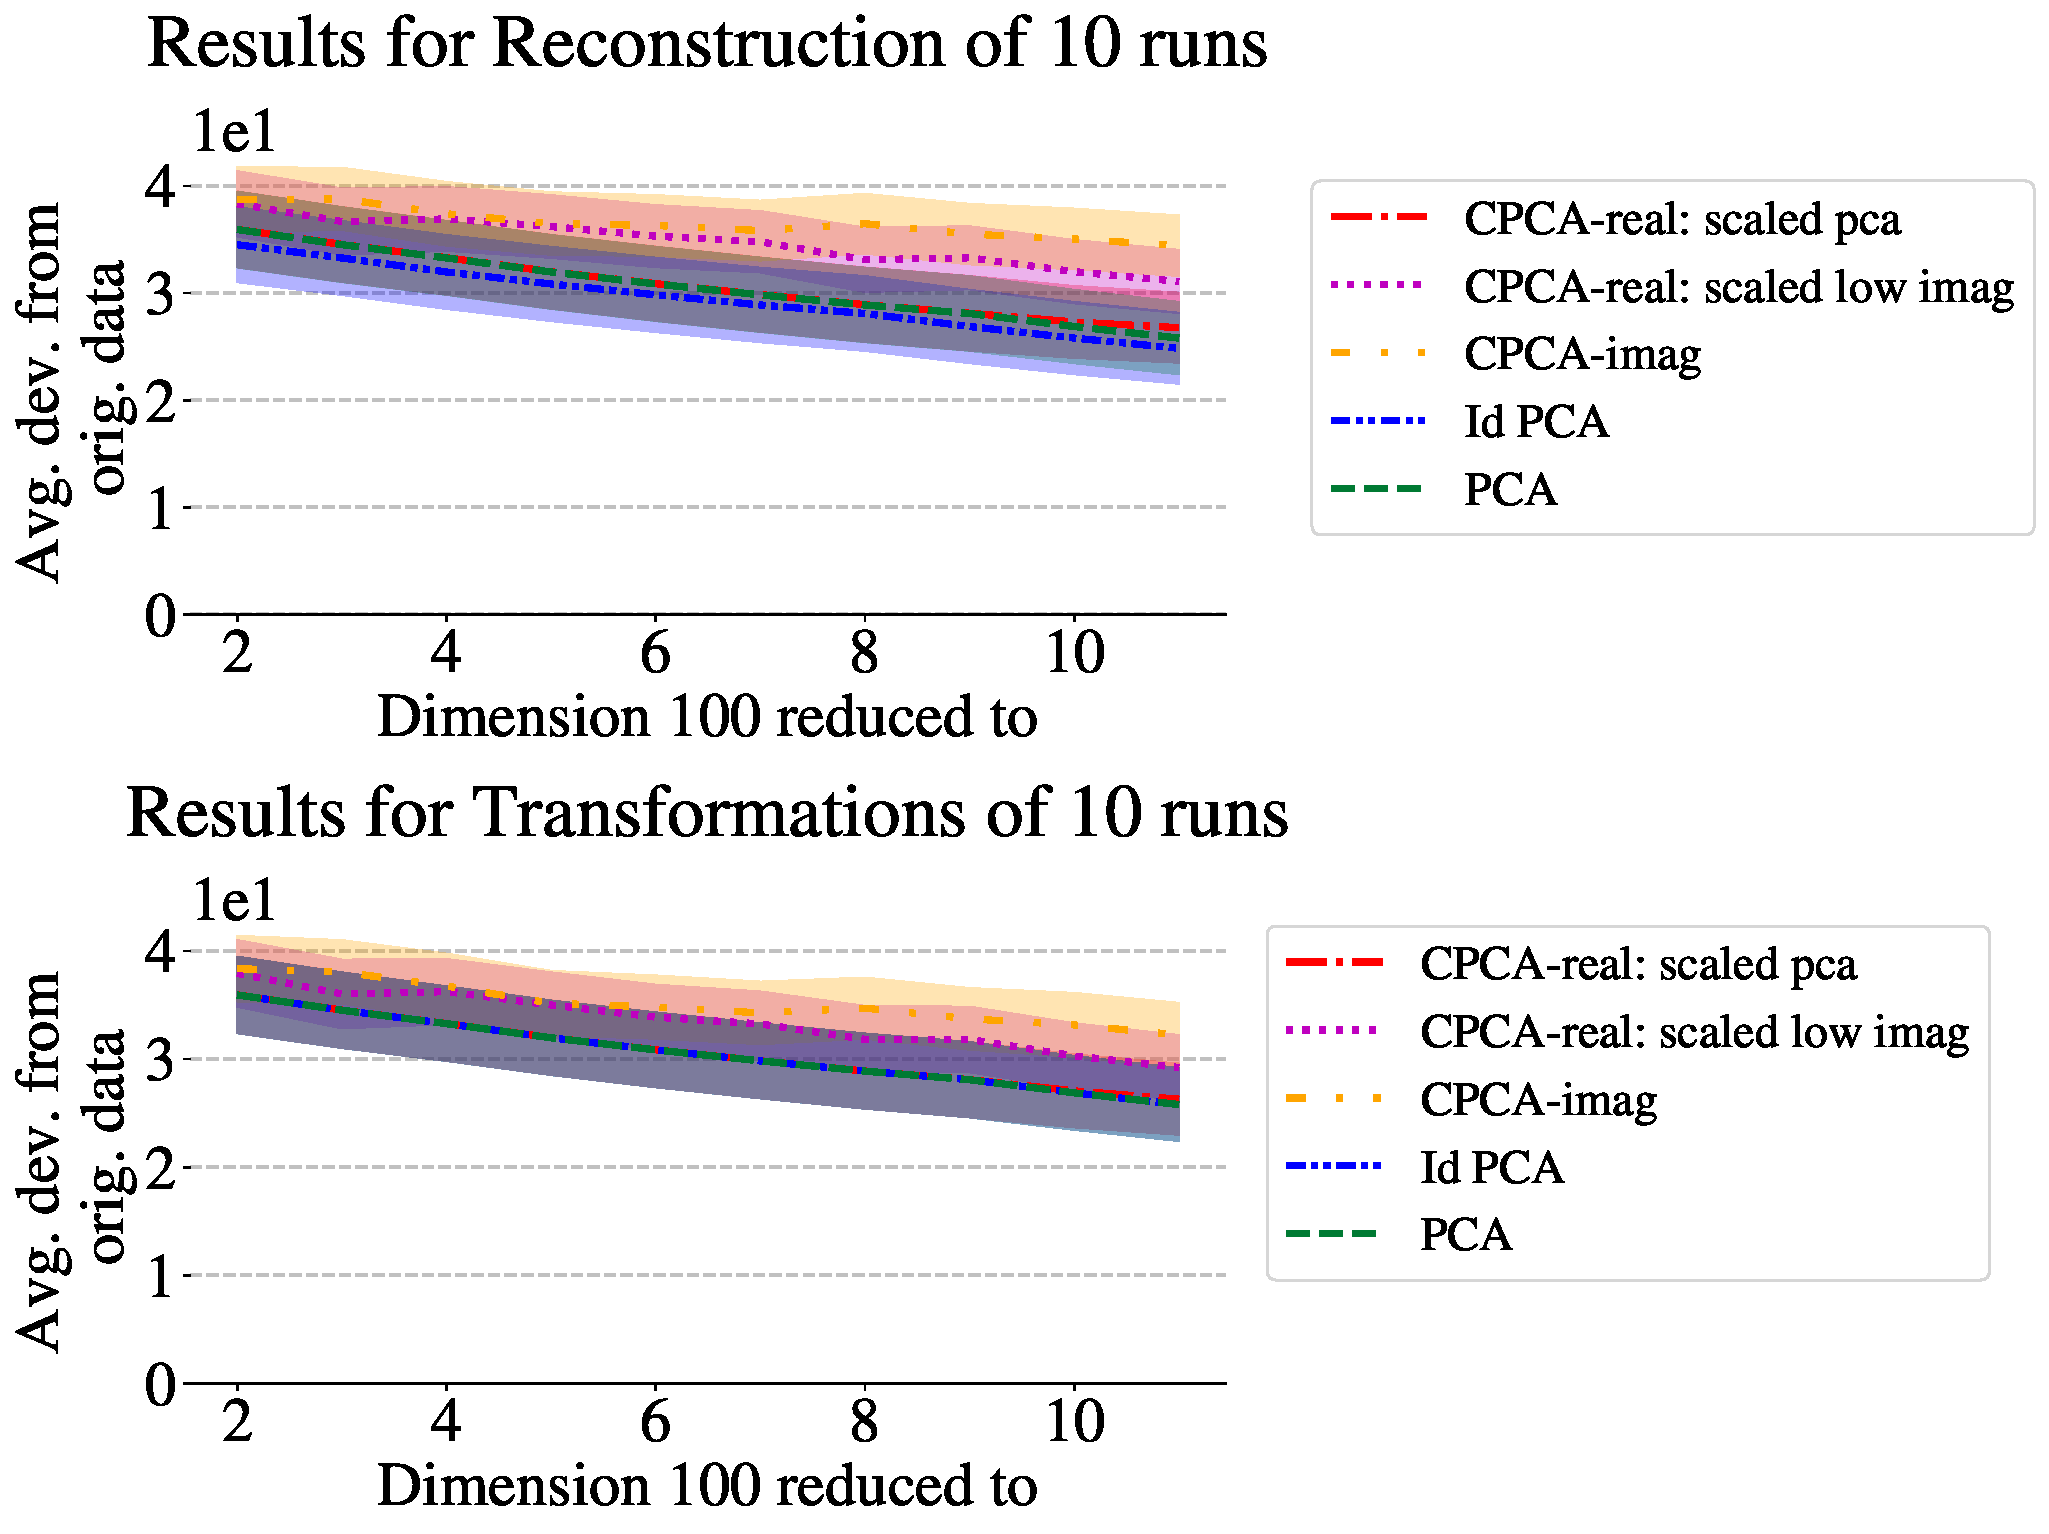
\includegraphics[width=7cm]{./images/multiple_runs/cpca/sep_lines/avg_dev_vs_dyn_low/5lines_100points_1neighbours_euclidean_cutk10.pdf}}
    \subfigure[Neighbour-Relation Measure]{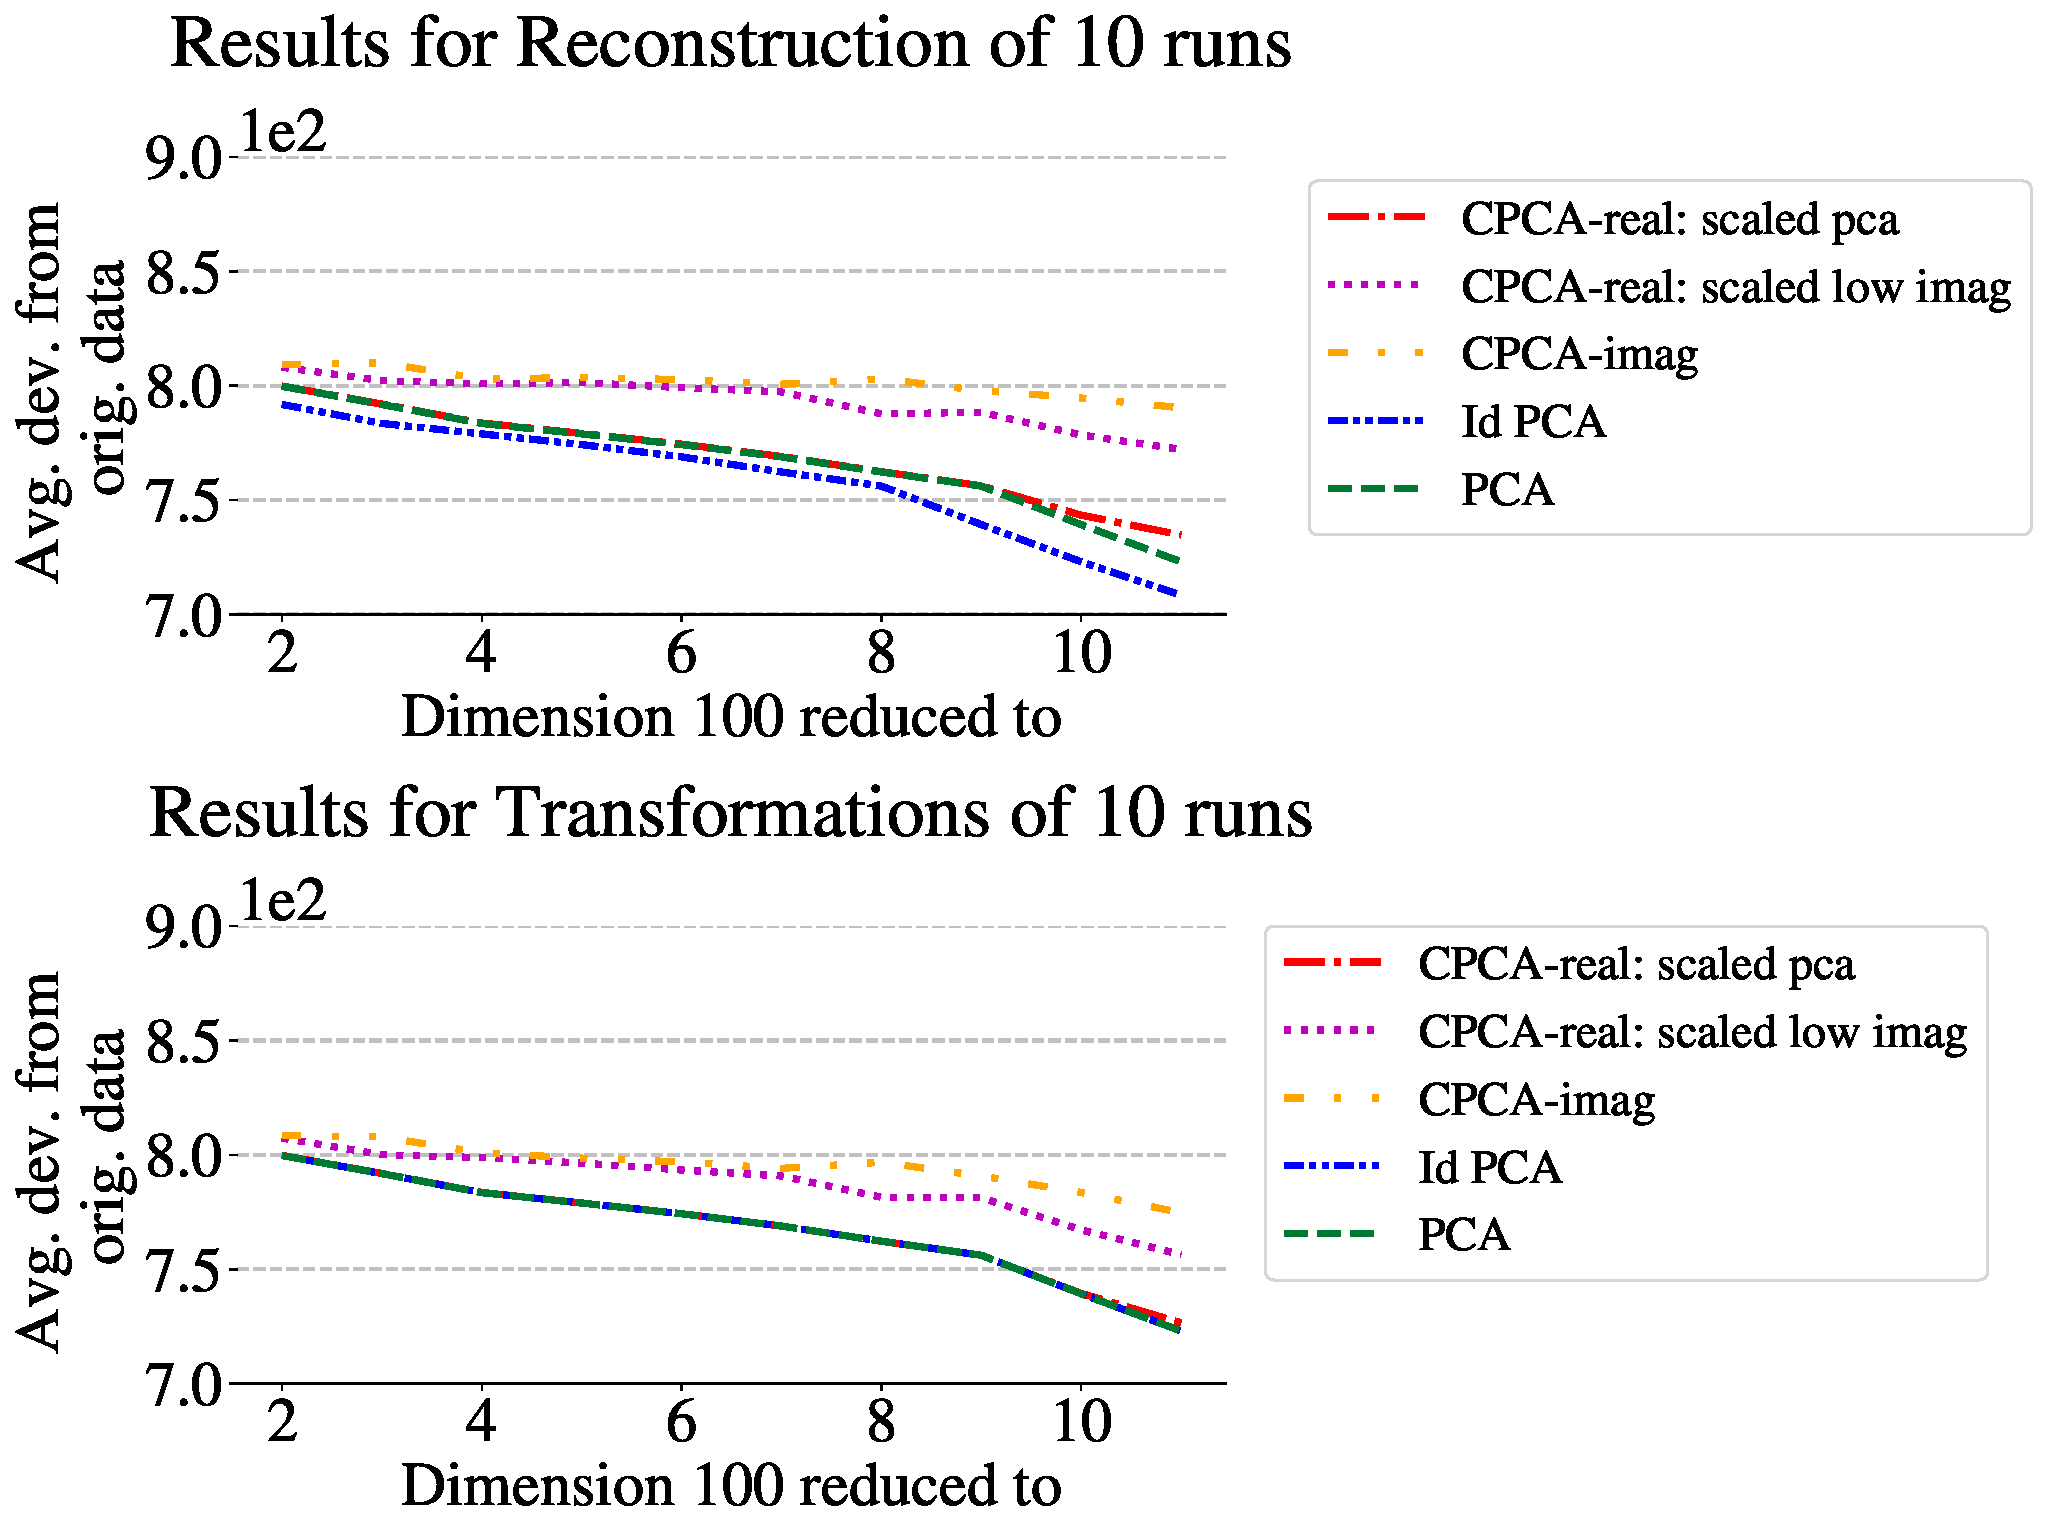
\includegraphics[width=7cm]{./images/multiple_runs/cpca/sep_lines/avg_dev_vs_dyn_low/5lines_100points_1neighbours_multiple_scalar_product_cutk10.pdf}}
    \caption{Results for data in separate lines for transformation dimensions between 2 and 10: comparing the summed distances between each predecessor and successor for data points in the original dataset and their reduced/reconstructed representations as dimensions increase}\label{fig:cpca-avg_dev_vs_high_dim-cut-seplines}
\end{figure}

All methods keep the order-based distances on separate lines similarly in both the reconstructed as well as the lower-dimensional embedding for both measures, see Figure~\ref{fig:cpca-avg_dev_vs_high_dim-seplines} and \ref{fig:cpca-avg_dev_vs_high_dim-cut-seplines}.

\FloatBarrier
\subsection{Exploration of Increasing Numbers of Neighbours}
To understand how the dimensionality reduction techniques impact the ordering of data points in a sequential data set, we explore in this experiment setting the quality of these techniques respective to an increasing number of predecessors and successors.
The data sets are reduced to dimensionality 2, as this dimensionality is often used to visualise data \cite{2d-often}.
Furthermore, we quantify the distances and relationships between the reconstructed as well as the transformed representation with the distances and relationships in the original data with an increasing number of neighbours for each run and present the averaged result.

\begin{figure}[htb!]
    \subfigure[Neighbour-Distance Measure]{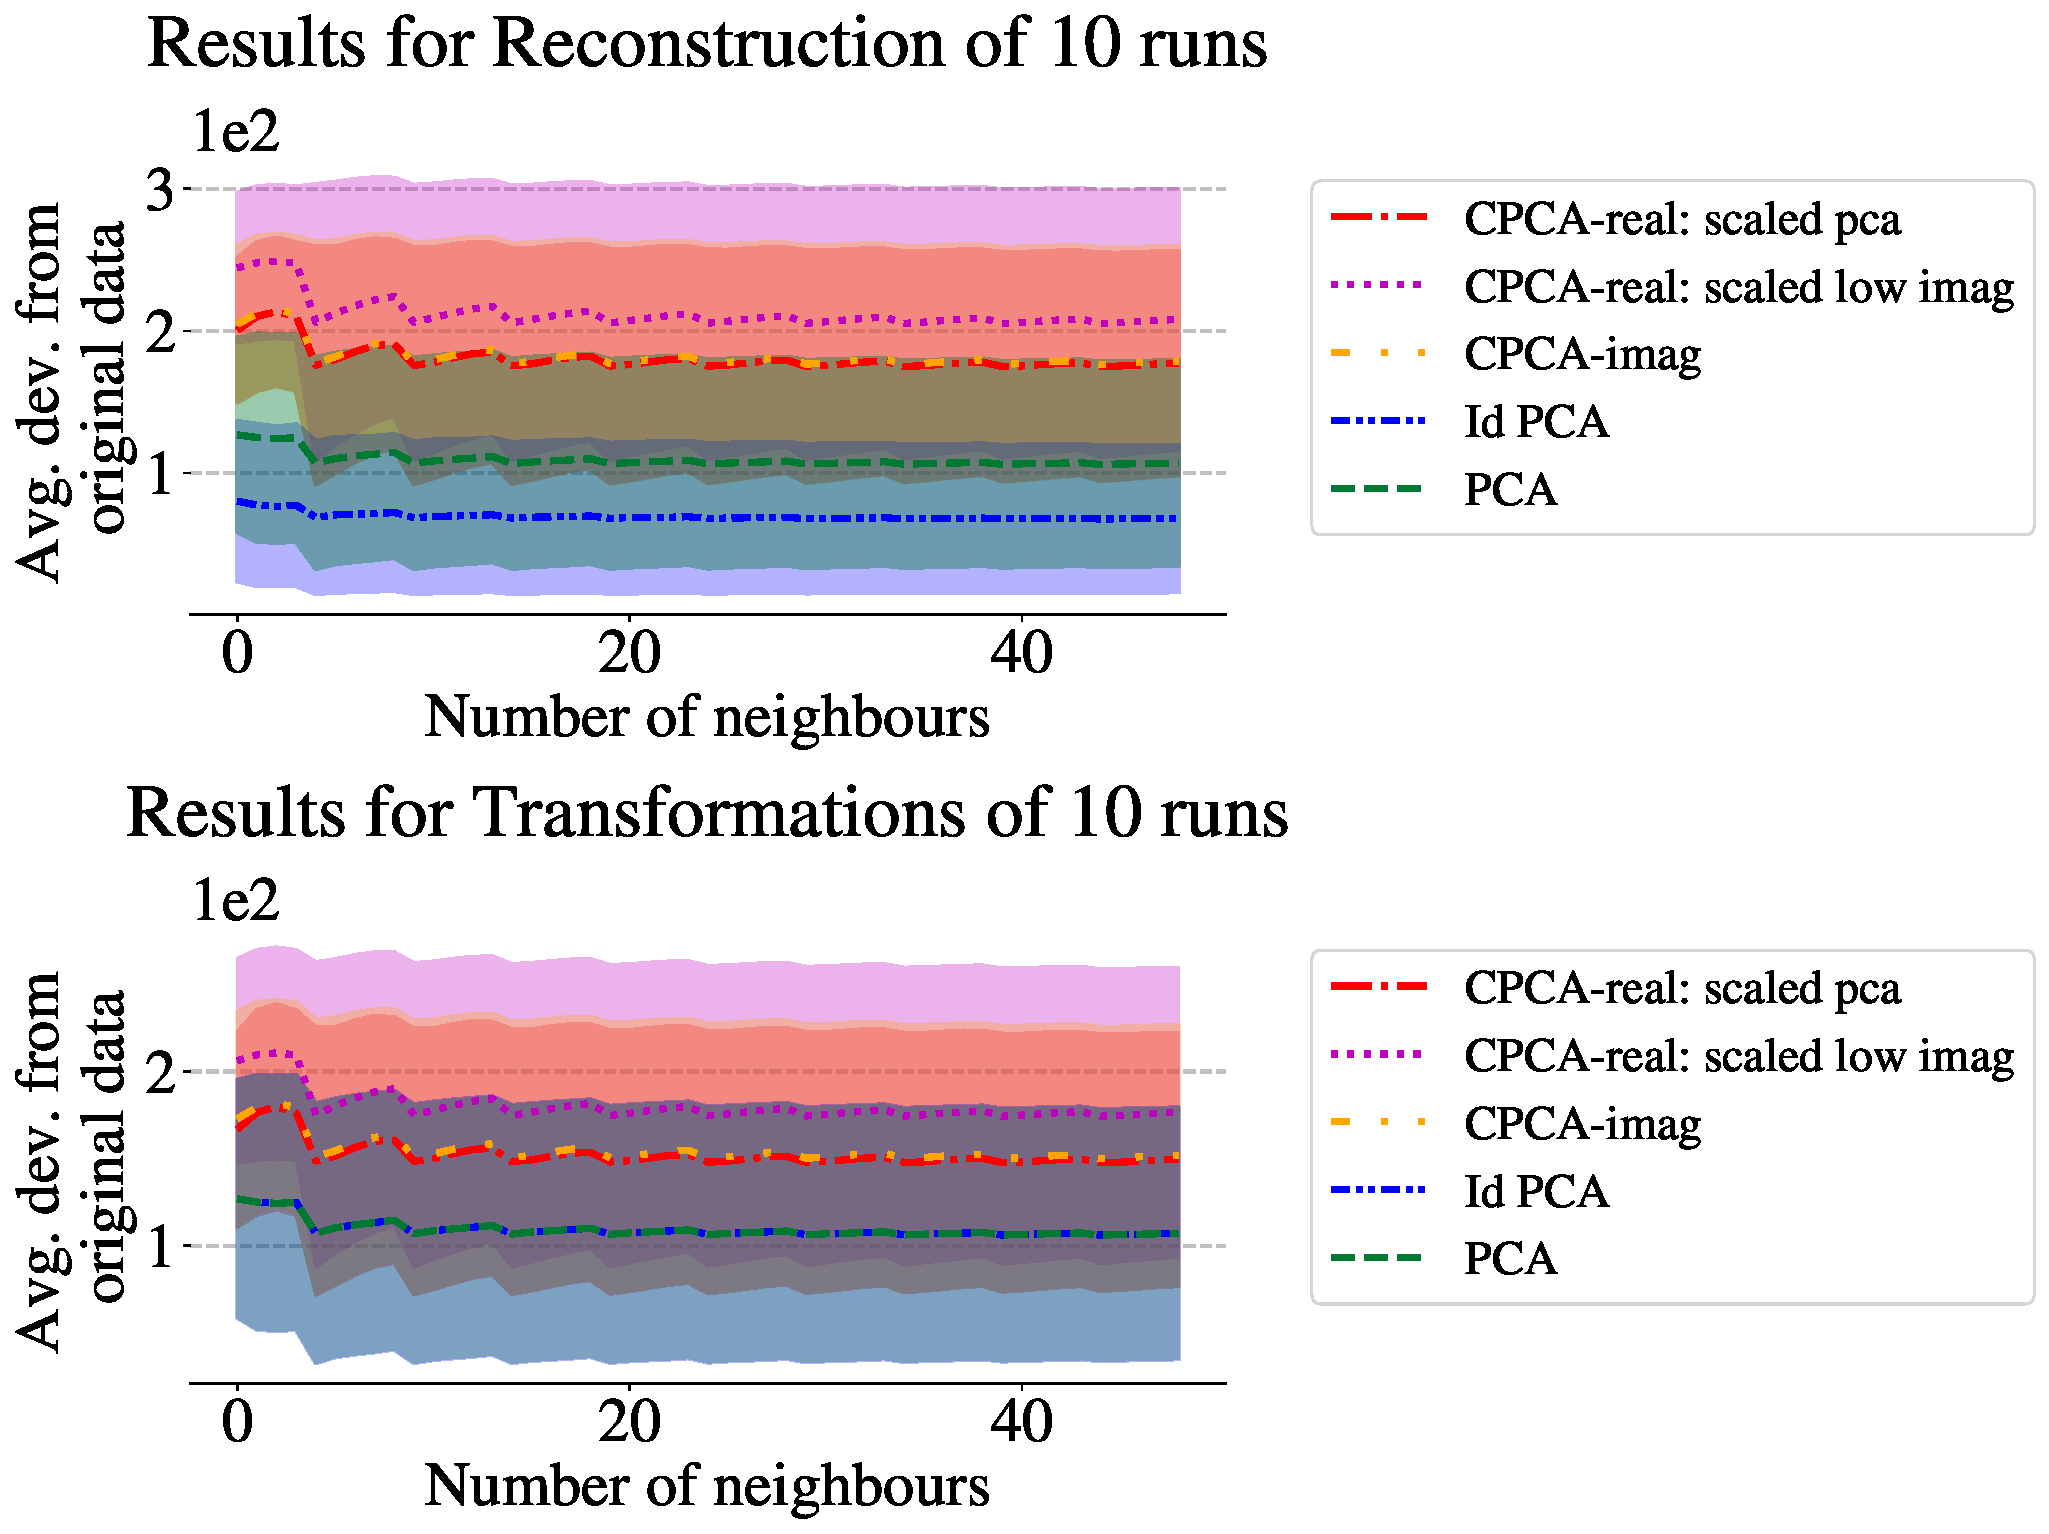
\includegraphics[width=7cm]{./images/multiple_runs/cpca/zigzag/num_neigh/5lines_100points_Noneneighbours_euclidean.pdf}}
    \subfigure[Neighbour-Relation Measure]{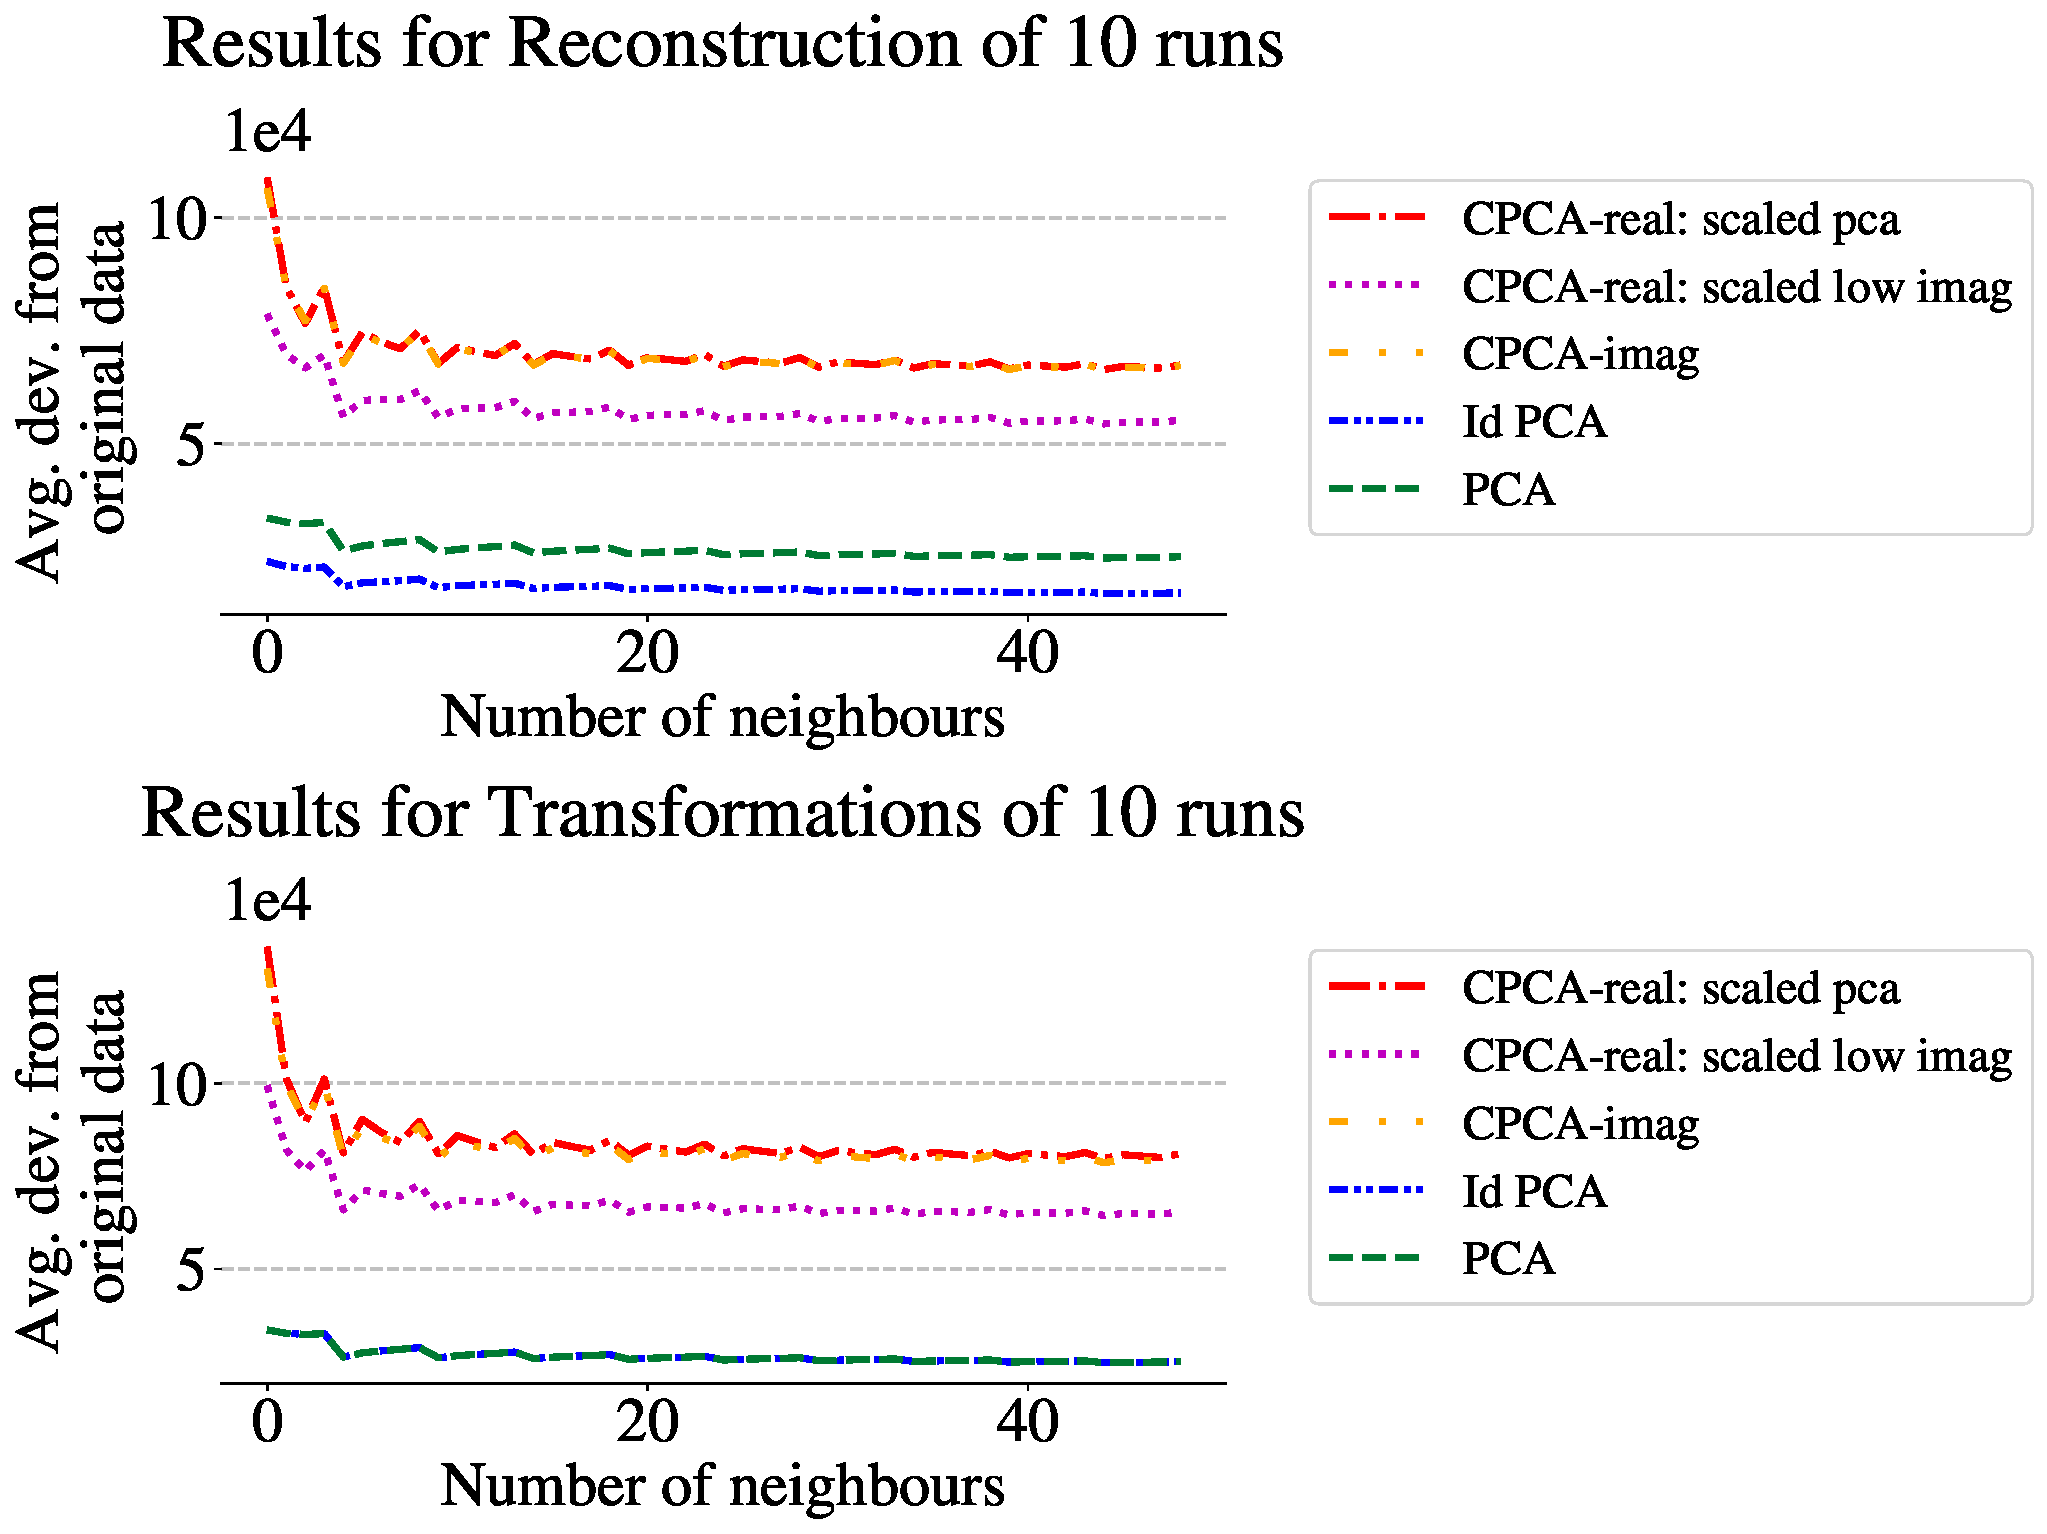
\includegraphics[width=7cm]{./images/multiple_runs/cpca/zigzag/num_neigh/5lines_100points_Noneneighbours_multiple_scalar_product.pdf}}
    \caption{Results for 10 runs for zigzag data: comparing the summed distances of an increasing number of predecessors and successors}\label{fig:cpca-num-neigh-zigzag}
\end{figure}

Similar to the previous experiment setting, the CPCA variants poorly maintain the relations and distances between each reconstructed and original as well as transformed and original data, see Figure~\ref{fig:cpca-num-neigh-zigzag}.
On the other hand, the result of Id PCA consistently outperforms PCA when comparing the distances and relationships between an increasing number of nearest neighbours in the sequence.
It preserves the distances and relationships equally well as PCA in the lower-dimensional space.
In Figure~\ref{fig:cpca-num_neigh_onelines}, we observe a high variance in the result for each variant for CPCA.
However, the means for all CPCA variants are roughly to those of PCA and Id PCA.
This trend also holds when comparing the relationships within the data using the MNR measure, where each dimensionality reduction method performs approximately similarly.

The same scenario is exhibited in Figure~\ref{fig:cpca_num_neigh-seplines}.
The variants of CPCA show high variance, but overall all methods maintain similar relations and distances in the sequences of the dataset.

\begin{figure}[htb!]
    \subfigure[Neighbour-Distance Measure]{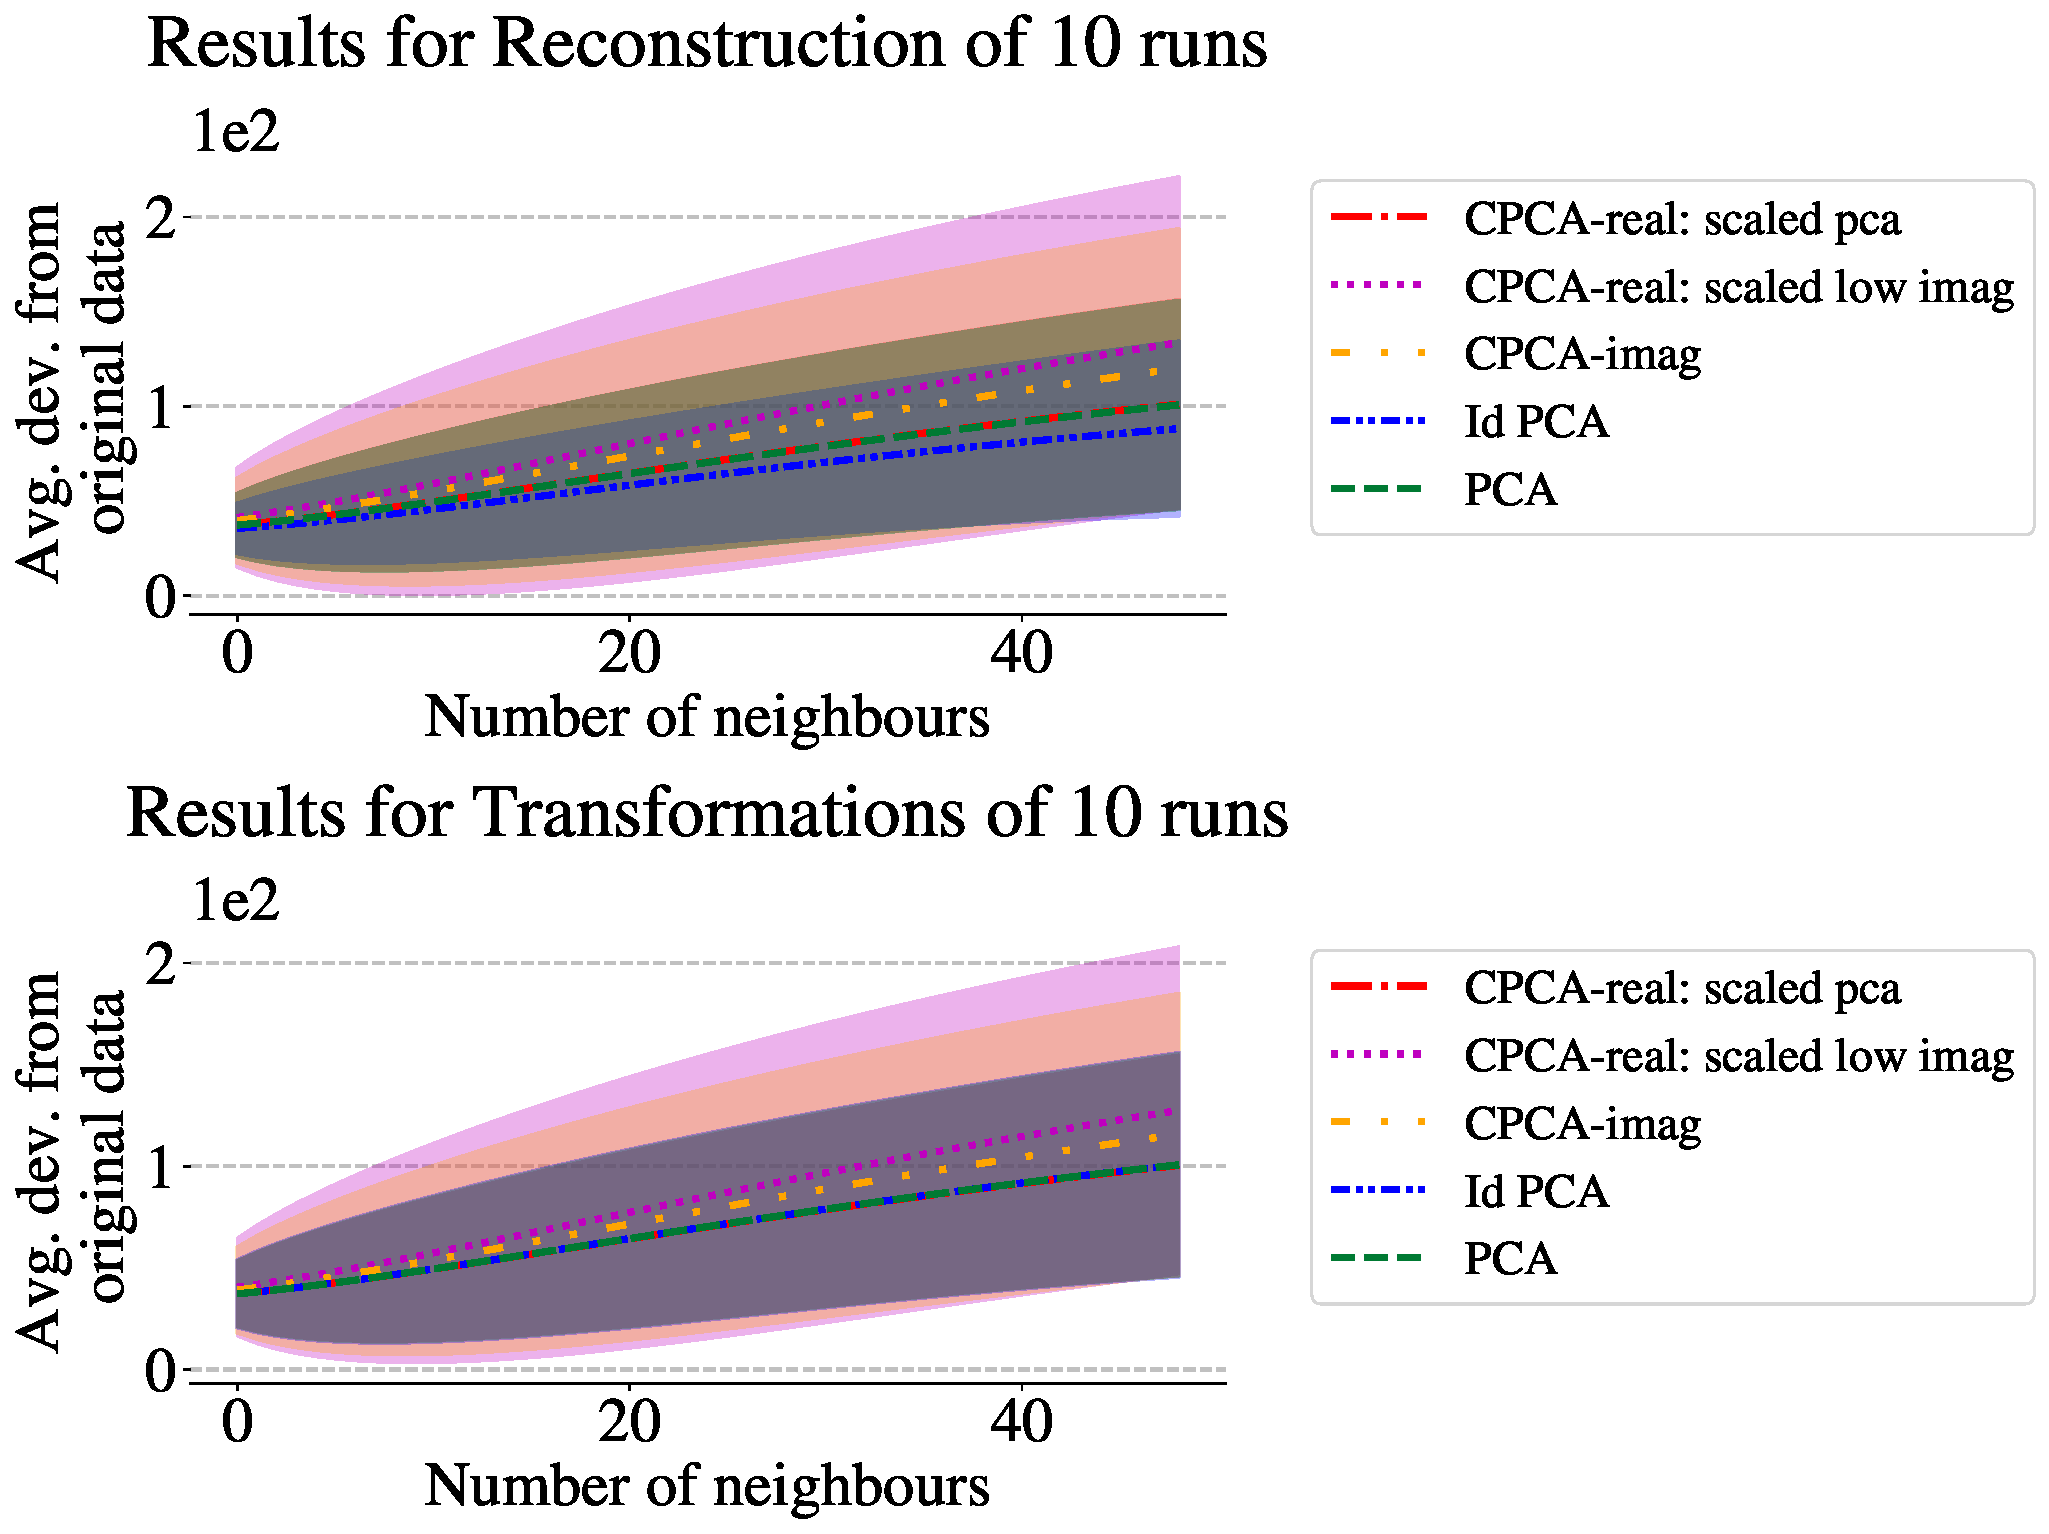
\includegraphics[width=7cm]{./images/multiple_runs/cpca/one_line/num_neigh/5lines_100points_Noneneighbours_euclidean.pdf}}
    \subfigure[Neighbour-Relation Measure]{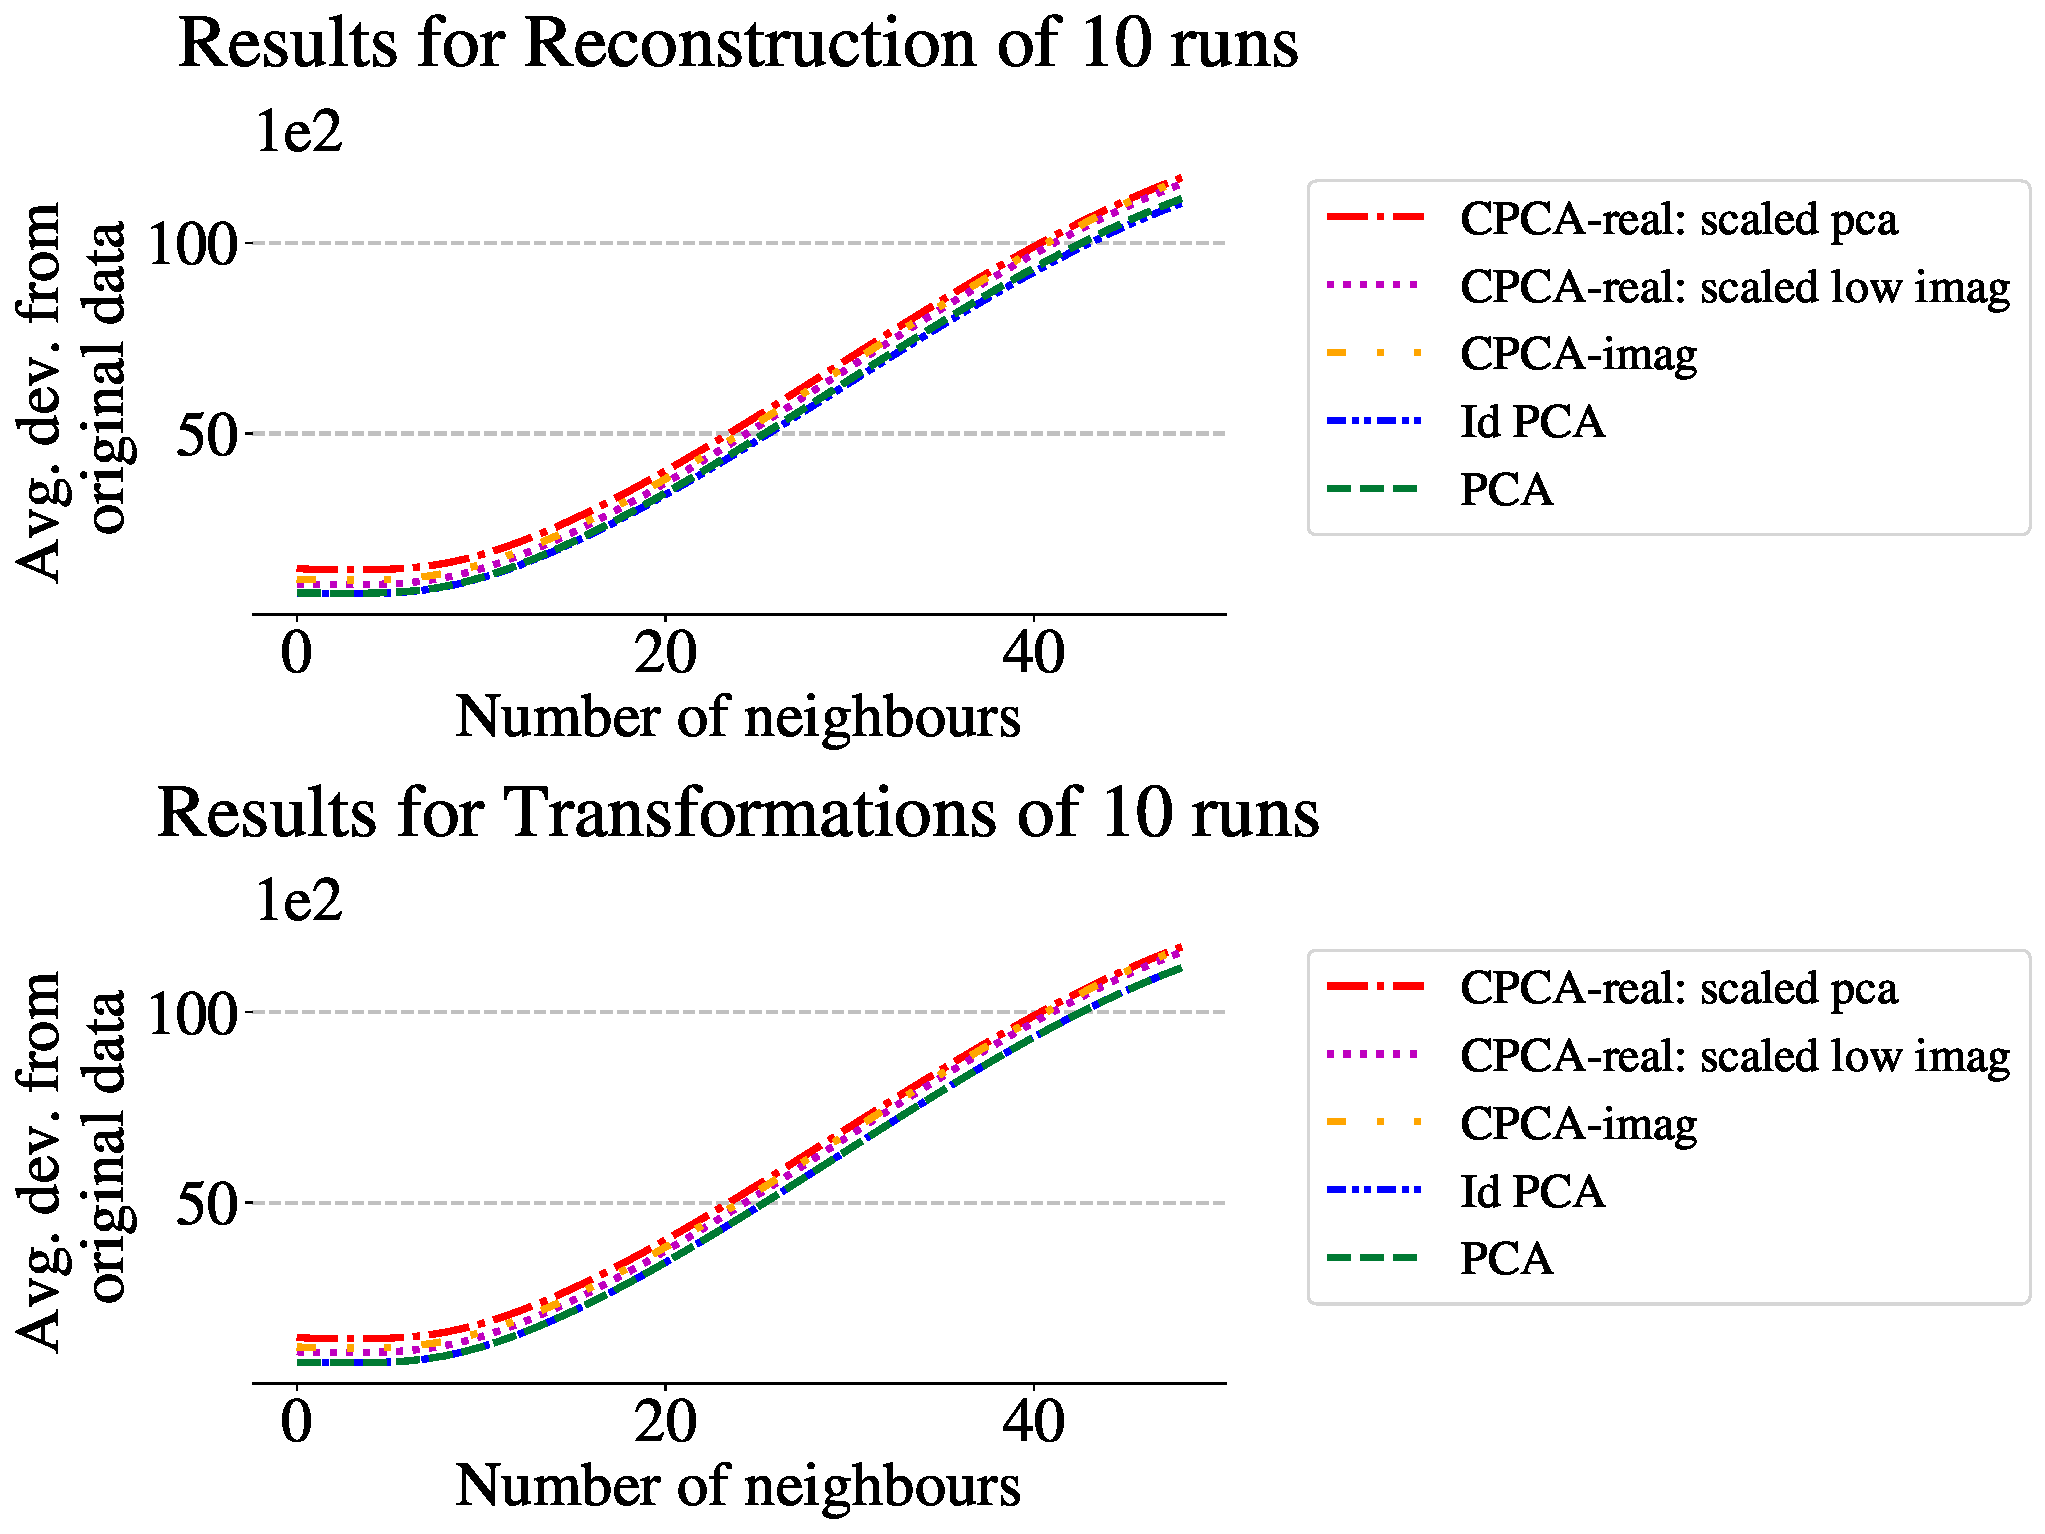
\includegraphics[width=7cm]{./images/multiple_runs/cpca/one_line/num_neigh/5lines_100points_Noneneighbours_multiple_scalar_product.pdf}}
    \caption{Results for 10 runs for smoothly ordered data: comparing the summed distances of an increasing number of predecessors and successors}\label{fig:cpca-num_neigh_onelines}
\end{figure}

\begin{figure}
    \subfigure[Neighbour-Distance Measure]{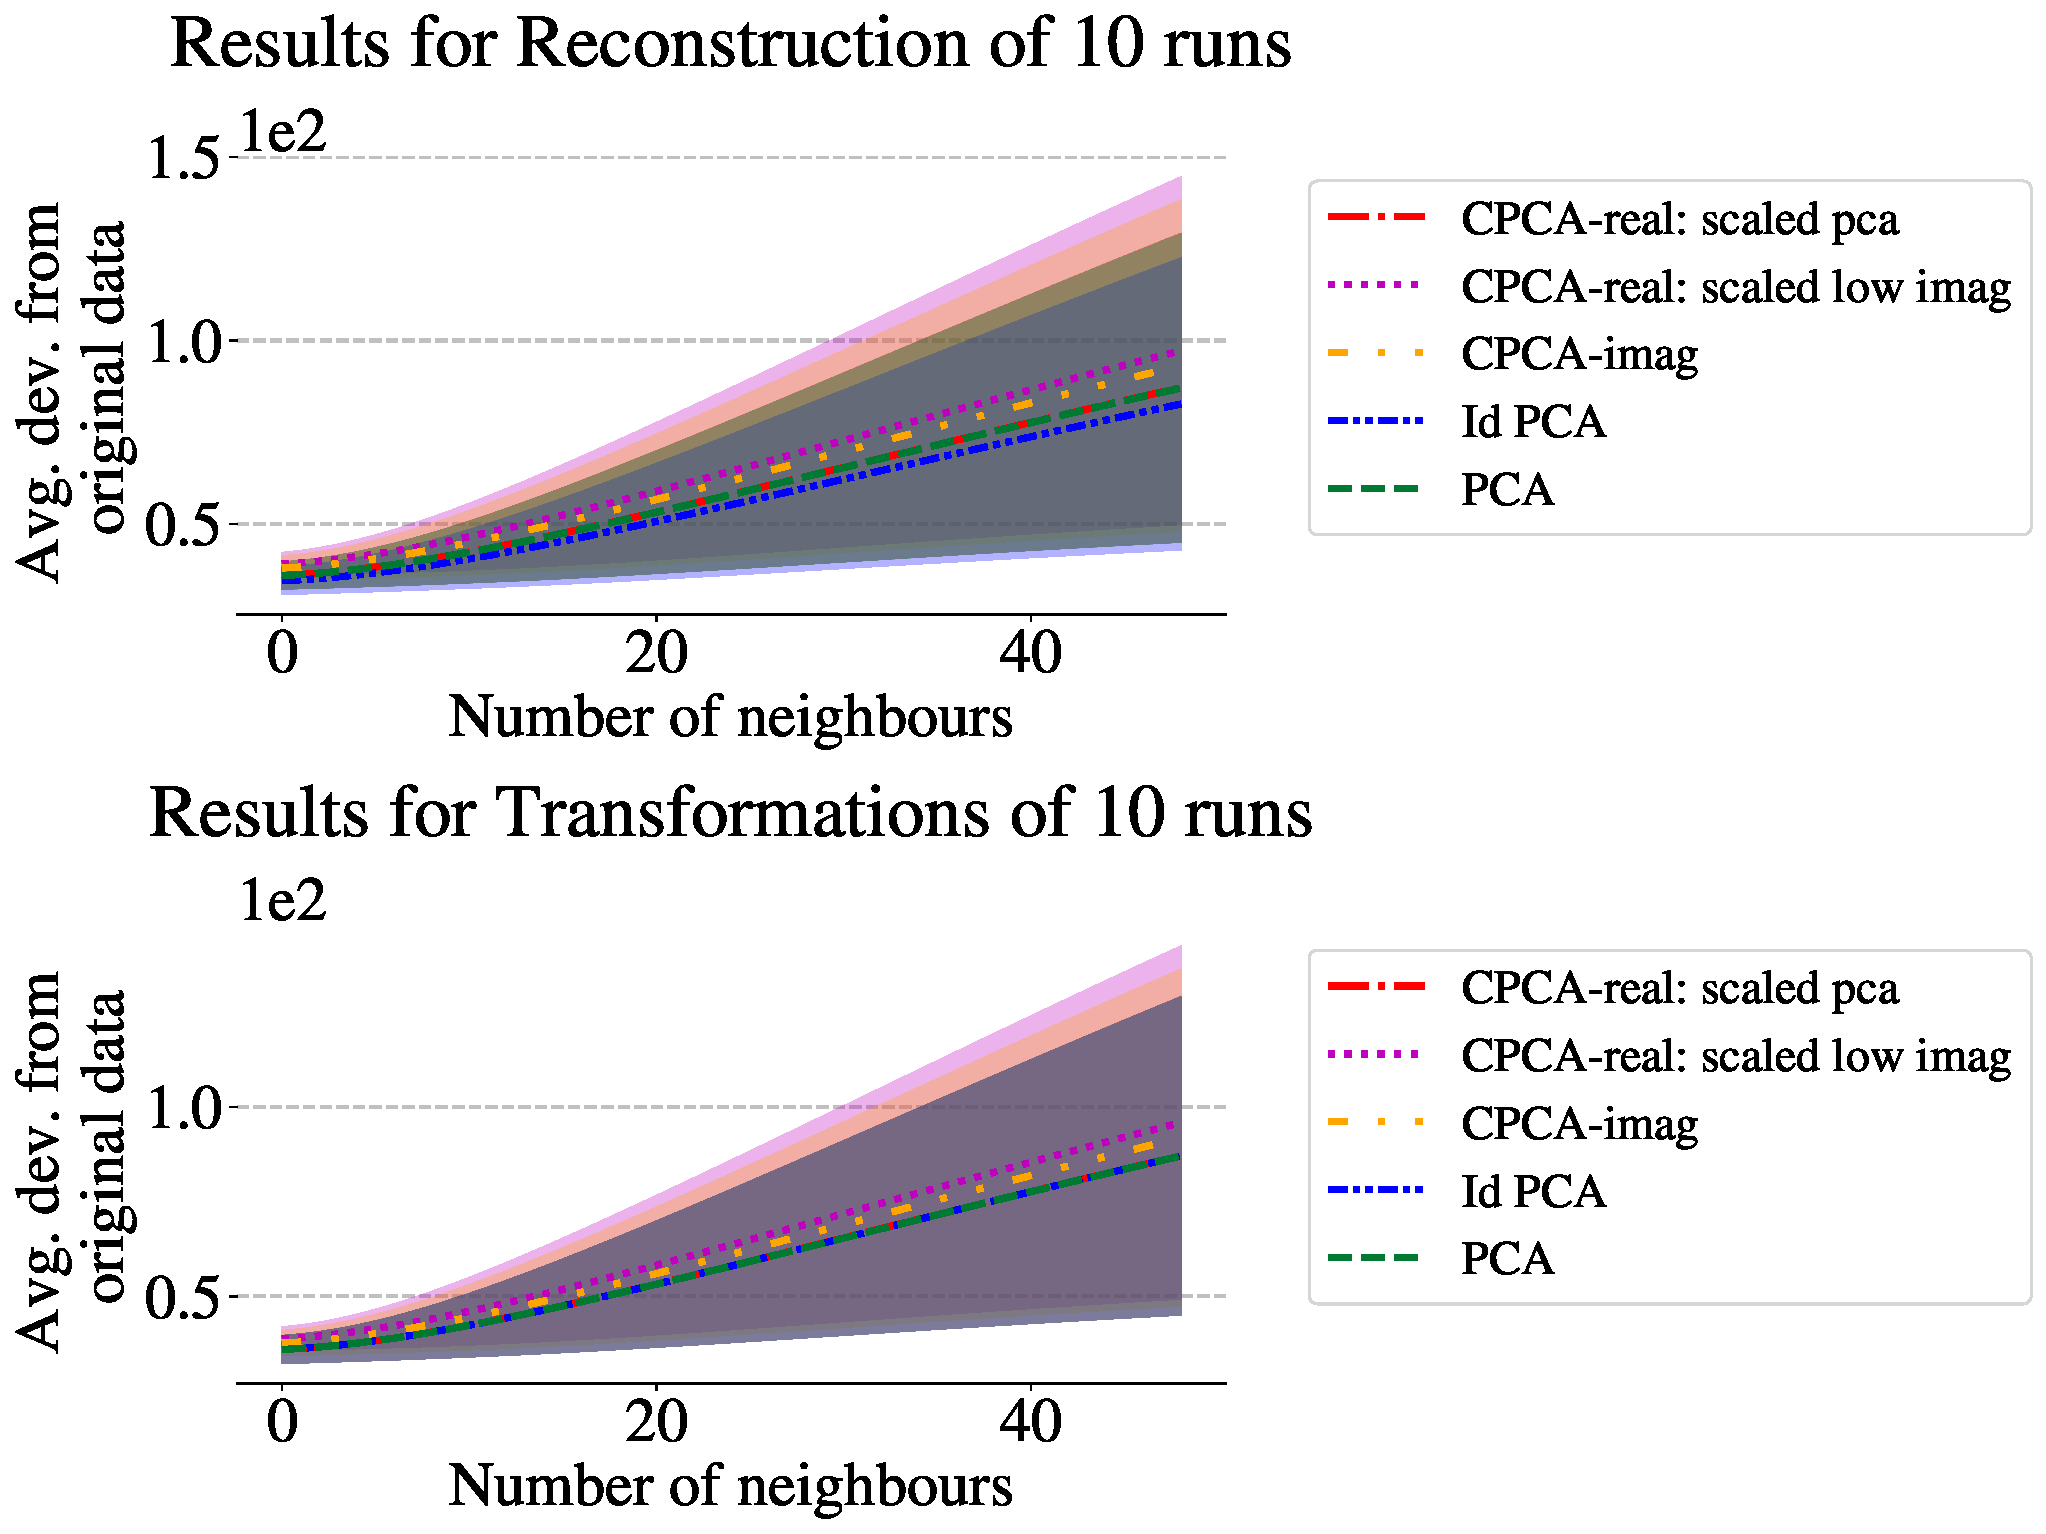
\includegraphics[width=7cm]{./images/multiple_runs/cpca/sep_lines/num_neigh/5lines_100points_Noneneighbours_euclidean.pdf}}
    \subfigure[Neighbour-Relation Measure]{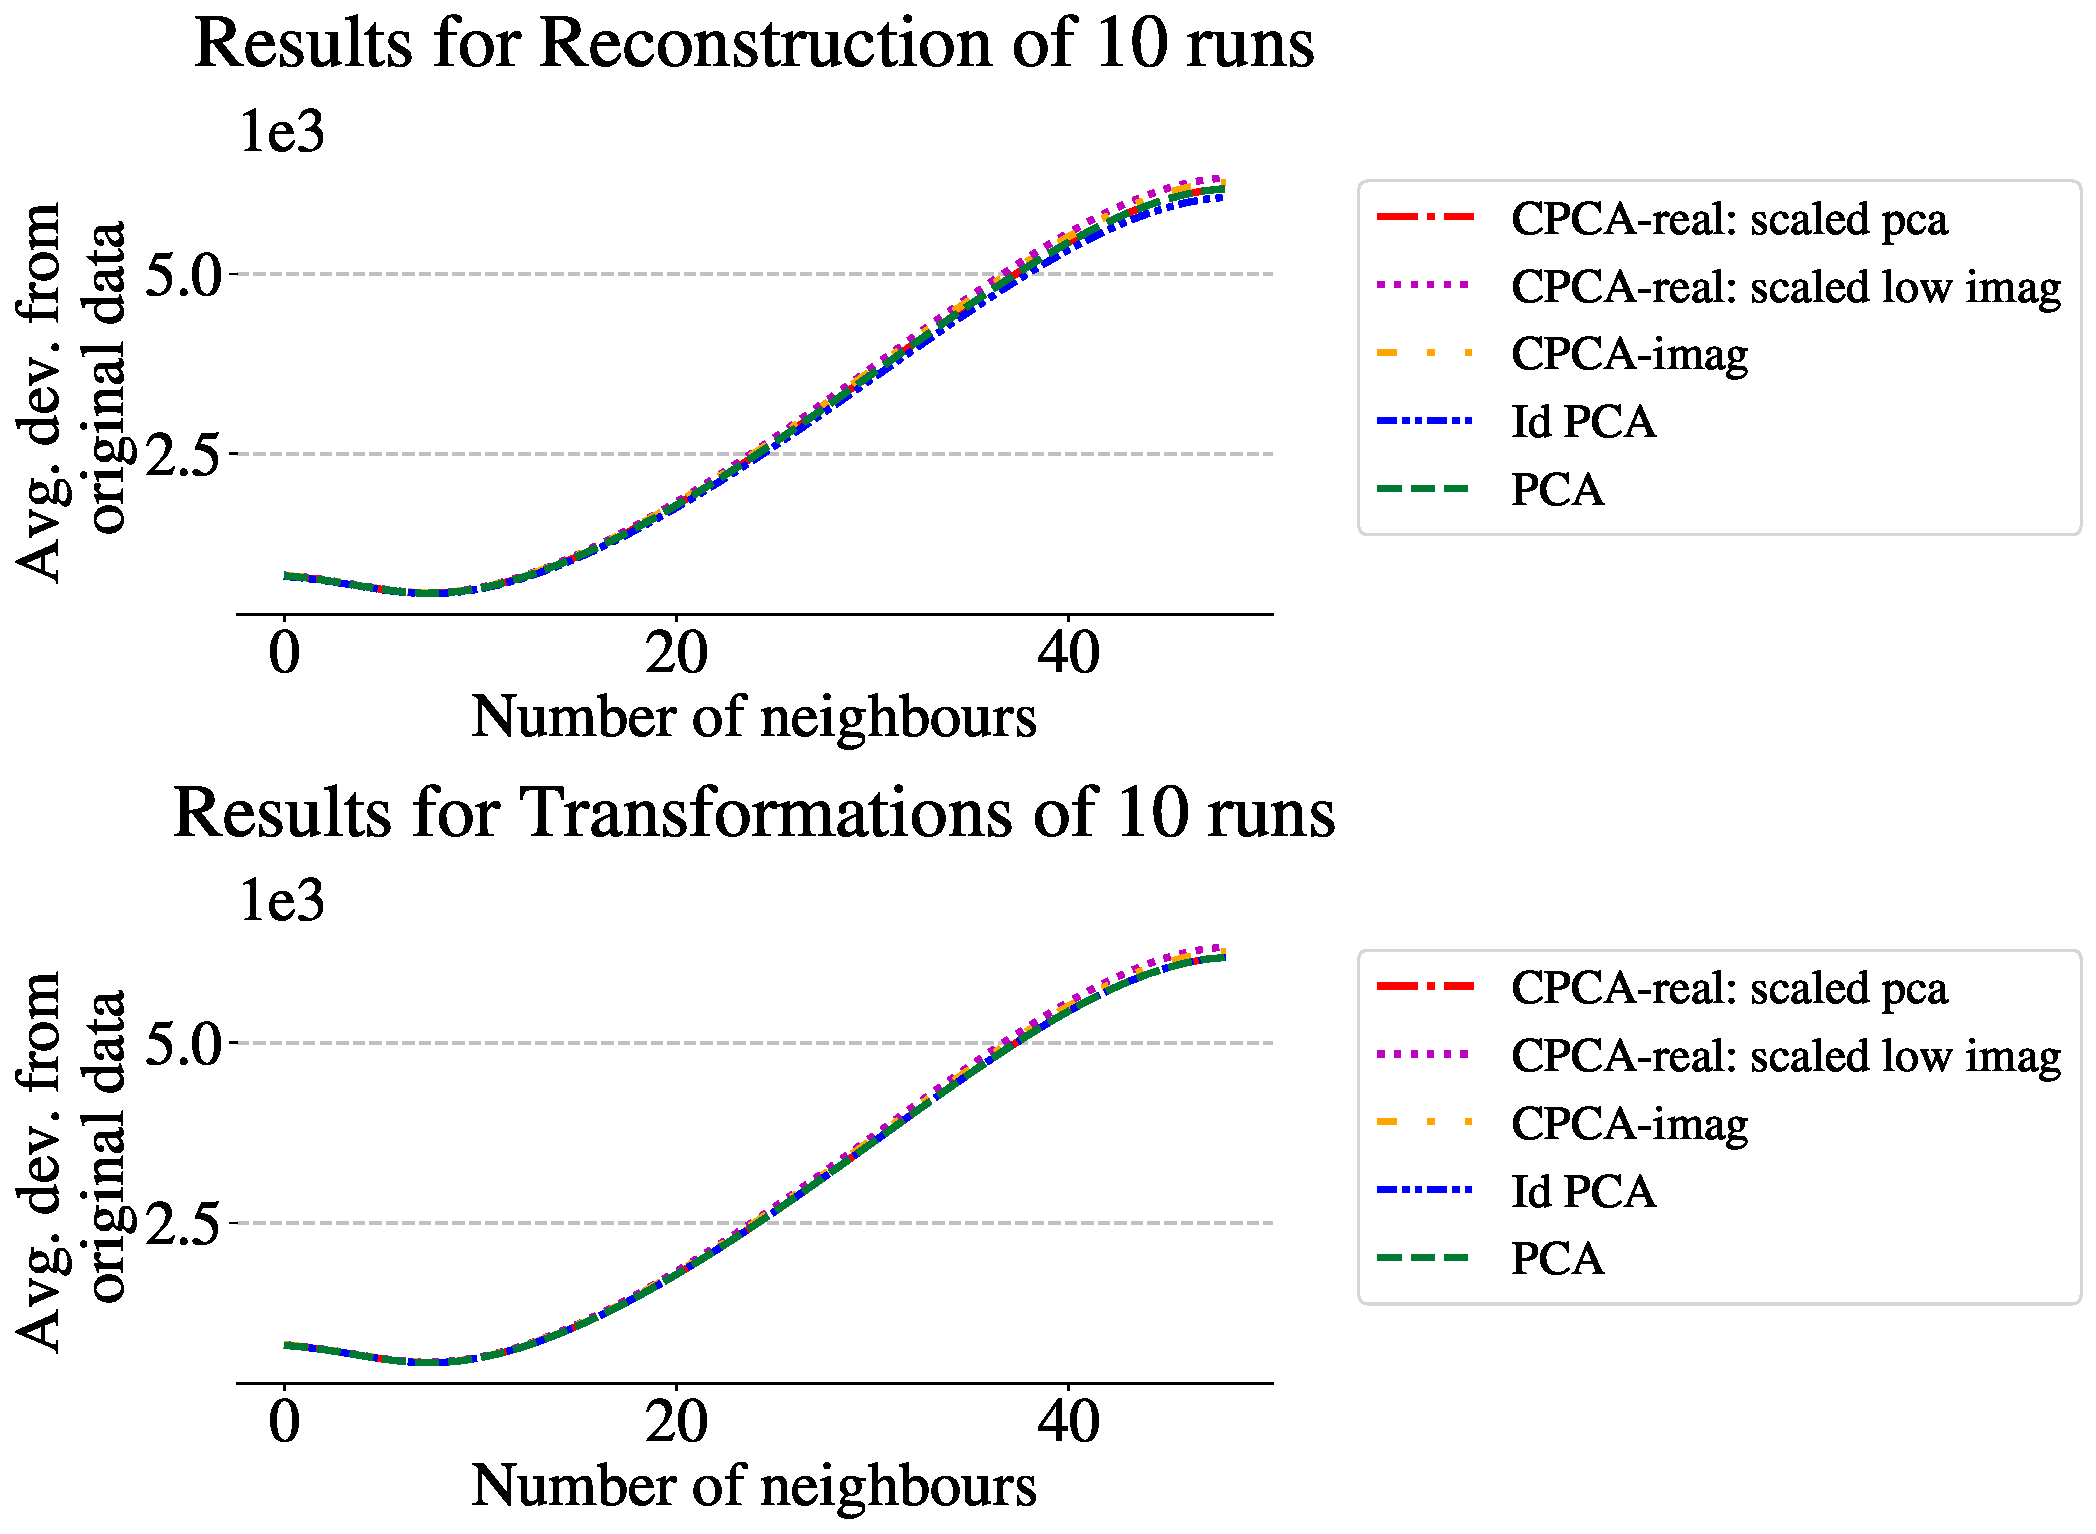
\includegraphics[width=7cm]{./images/multiple_runs/cpca/sep_lines/num_neigh/5lines_100points_Noneneighbours_multiple_scalar_product.pdf}}
    \caption{Results for data in separate lines: comparing the summed distances of an increasing number of predecessors and successors}\label{fig:cpca_num_neigh-seplines}
\end{figure}

\FloatBarrier

\subsection{Analysis of Growing Numbers of Neighbours and Transformation Dimensions}
In this experiment, we combine the previous experiments to explore the effects of reducing dimensionality to a growing number of dimensions while also increasing the number of neighbours examined compared to the original dataset.

Applying Id PCA, PCA and the variants of CPCA to zigzag data in this setting yields the results visualised in Figure~\ref{fig:cpca-num_neigh_vs_dyn_low-zigzag-euclidean} quantified by the ND measure.
We observe that while the results of the CPCA variants show slightly better order-based distance preservation in the transformational representation than the preservation in the reconstructed embedding, they are still inferior to the results of PCA and Id PCA.
Furthermore, we see the impact of the zigzag order of the data.
All CPCA variants maintain order-based distances somewhat poorly up to the four nearest predecessors and four nearest successors.
These data points do not lie on the same lines.
However, when comparing the five nearest neighbours in each direction of the sequence, we see an improvement.
This is because every fifth predecessor and successor lie on the same line as data was generated on five lines.
Analogously to the previous section, we observe that Id PCA performs slightly better than PCA in two dimensions in the reconstructed embedding.

We find a similar pattern when measuring the relations between a growing number of nearest neighbours in a sequence while transforming to an increasing number of dimensions, measured by MNR, see Figure~\ref{fig:cpca-num_neigh_vs_dyn_low-zigzag-mscal}.
For each CPCA variant, we notice a marginally better result for dimensionality 2, indicating a higher quality of order-based relation preservation than in higher dimensions.
Interestingly, all CPCA variants face significant challenges in maintaining order-based relations with the immediate predecessor and successor.

Applying the variants of CPCA to smoothly ordered data yields a similar result for all dimensionality reduction methods, with a worse result for \textit{CPCA-real+low imag} and \textit{CPCA-imag}, see Figure~\ref{fig:cpca-num_neigh_vs_dyn_low-oneline-euclidean}.

However, when evaluating the same transformations and reconstructions using the MNR measure, as shown in Figure~\ref{fig:cpca-num_neigh_vs_dyn_low-oneline-mscal}, we observe different outcomes.
Id PCA and PCA exhibit similar performance in maintaining relations within the data, whereas \textit{CPCA-imag} and \textit{CPCA-real+low imag} show slightly lower performances.
\textit{CPCA-real+scaled pca} underperforms in comparison to the other techniques.
Across all variants of CPCA, we notice that they better maintain relations within the data when the number of transformed dimensions is lower, while the number of neighbours does not significantly impact their performance.

PCA, \textit{CPCA real+aligned PCA} and Id PCA exhibit similar performance in preserving distances within consecutive data points in multiple sequences, as shown in Figure~\ref{fig:cpca-num_neigh_vs_dyn_low-seplines-euclidean}.
However, \textit{CPCA real+low imag} and \textit{CPCA imag} show comparatively less favourable results.
All of the tested techniques improve their performance, as the number of dimensions used for data transformation increases, while the quality tends to decrease with a growing number of neighbours.


Interestingly, both \textit{CPCA real+low imag} and \textit{CPCA imag} exhibit superior preservation of the Multiple-Neighbour-Relation (MNR) measure as the number of neighbours increases, in contrast to PCA, Id PCA and \textit{CPCA real+scaled PCA}, as depicted in Figure~\ref{fig:cpca-num_neigh_vs_dyn_low-seplines-mscal}.
This suggests that although the Euclidean distances are not as well preserved in comparison to PCA, the CPCA variants that retain a substantial part of their imaginary component, excel in preserving relations between up to 10 neighbours better than the other methods.
PCA, Id PCA and \textit{CPCA real+scaled PCA} follow a similar pattern: they exhibit suboptimal preservation of relations for up to four dimensions and for more than seven neighbouring data points in both directions of the sequences.
It is logical that these methods perform better in higher dimensions, as higher-dimensional transformations allow for the retention of more information but it is surprising that this stops the more neighbours we examine.

\begin{figure}
    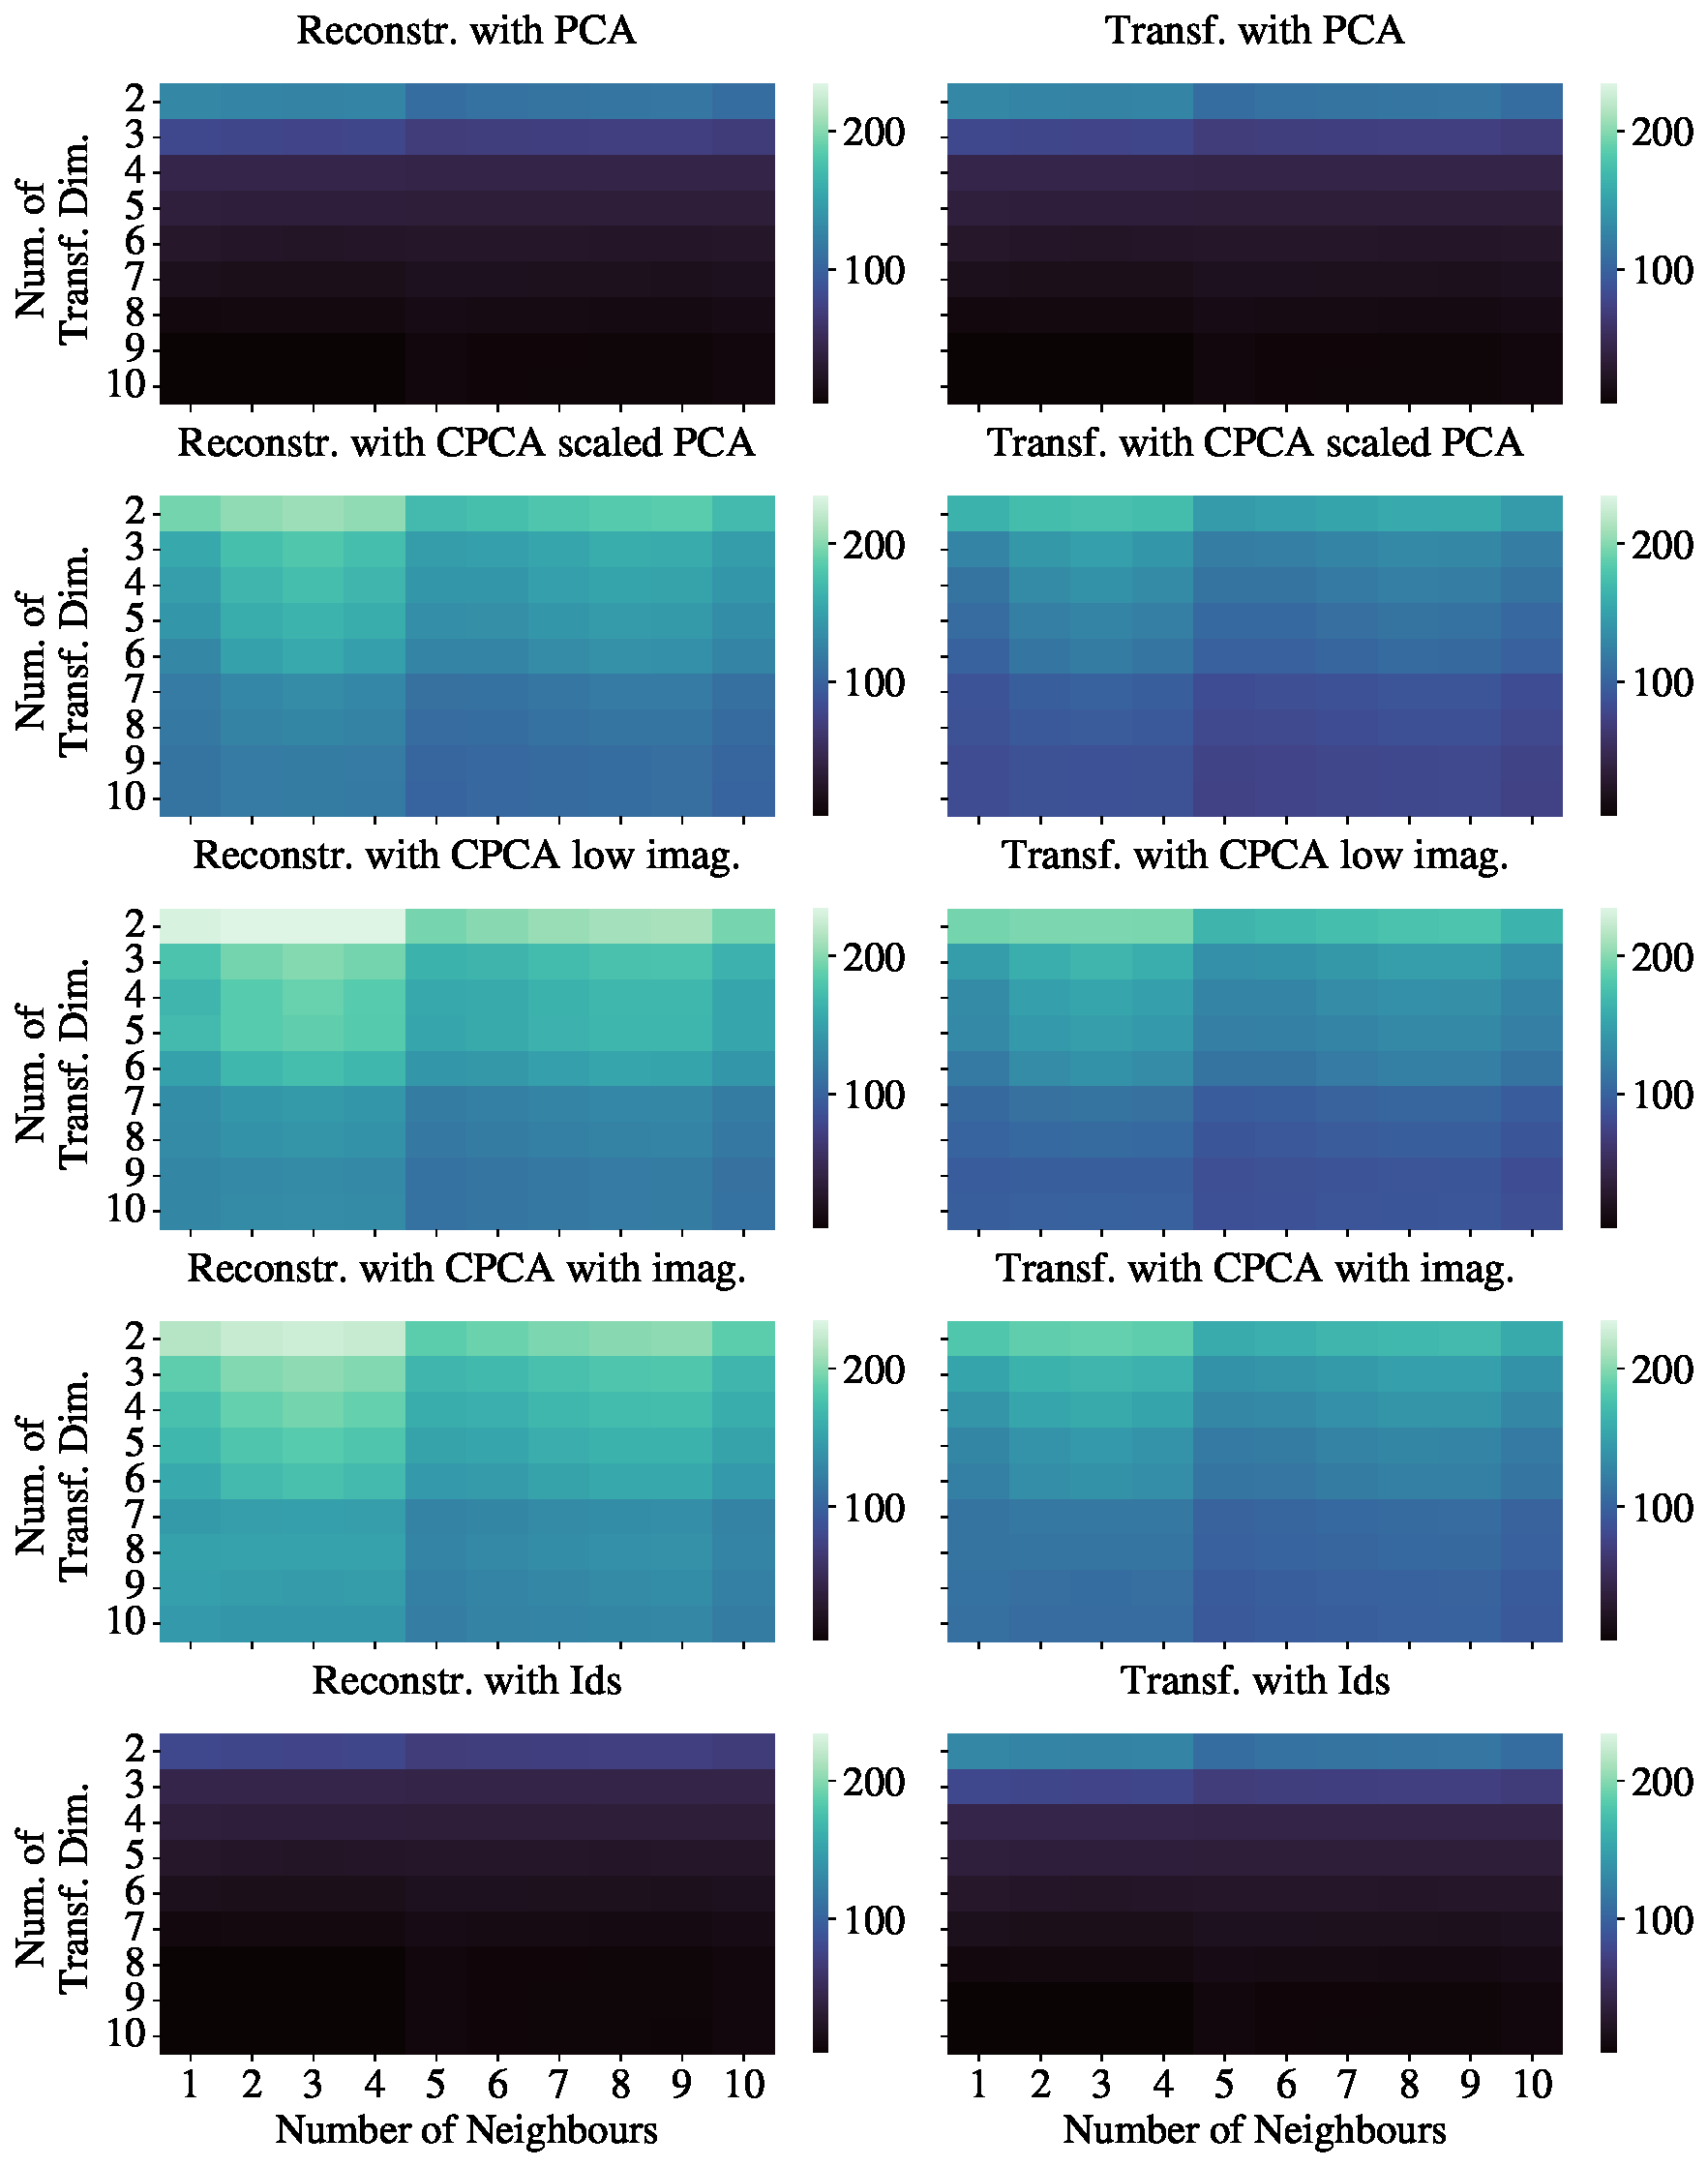
\includegraphics[width = \textwidth]{images/multiple_runs/cpca/zigzag/num_neigh_vs_dyn_low/euclidean_10runs_5lines_100points_10neighbours.pdf}
    \caption{Neighbour-Distance measure on zigzag data: comparing the results
     for increasing numbers of neighbours and dimensionality of the transformed space} \label{fig:cpca-num_neigh_vs_dyn_low-zigzag-euclidean}
\end{figure}

\begin{figure}
    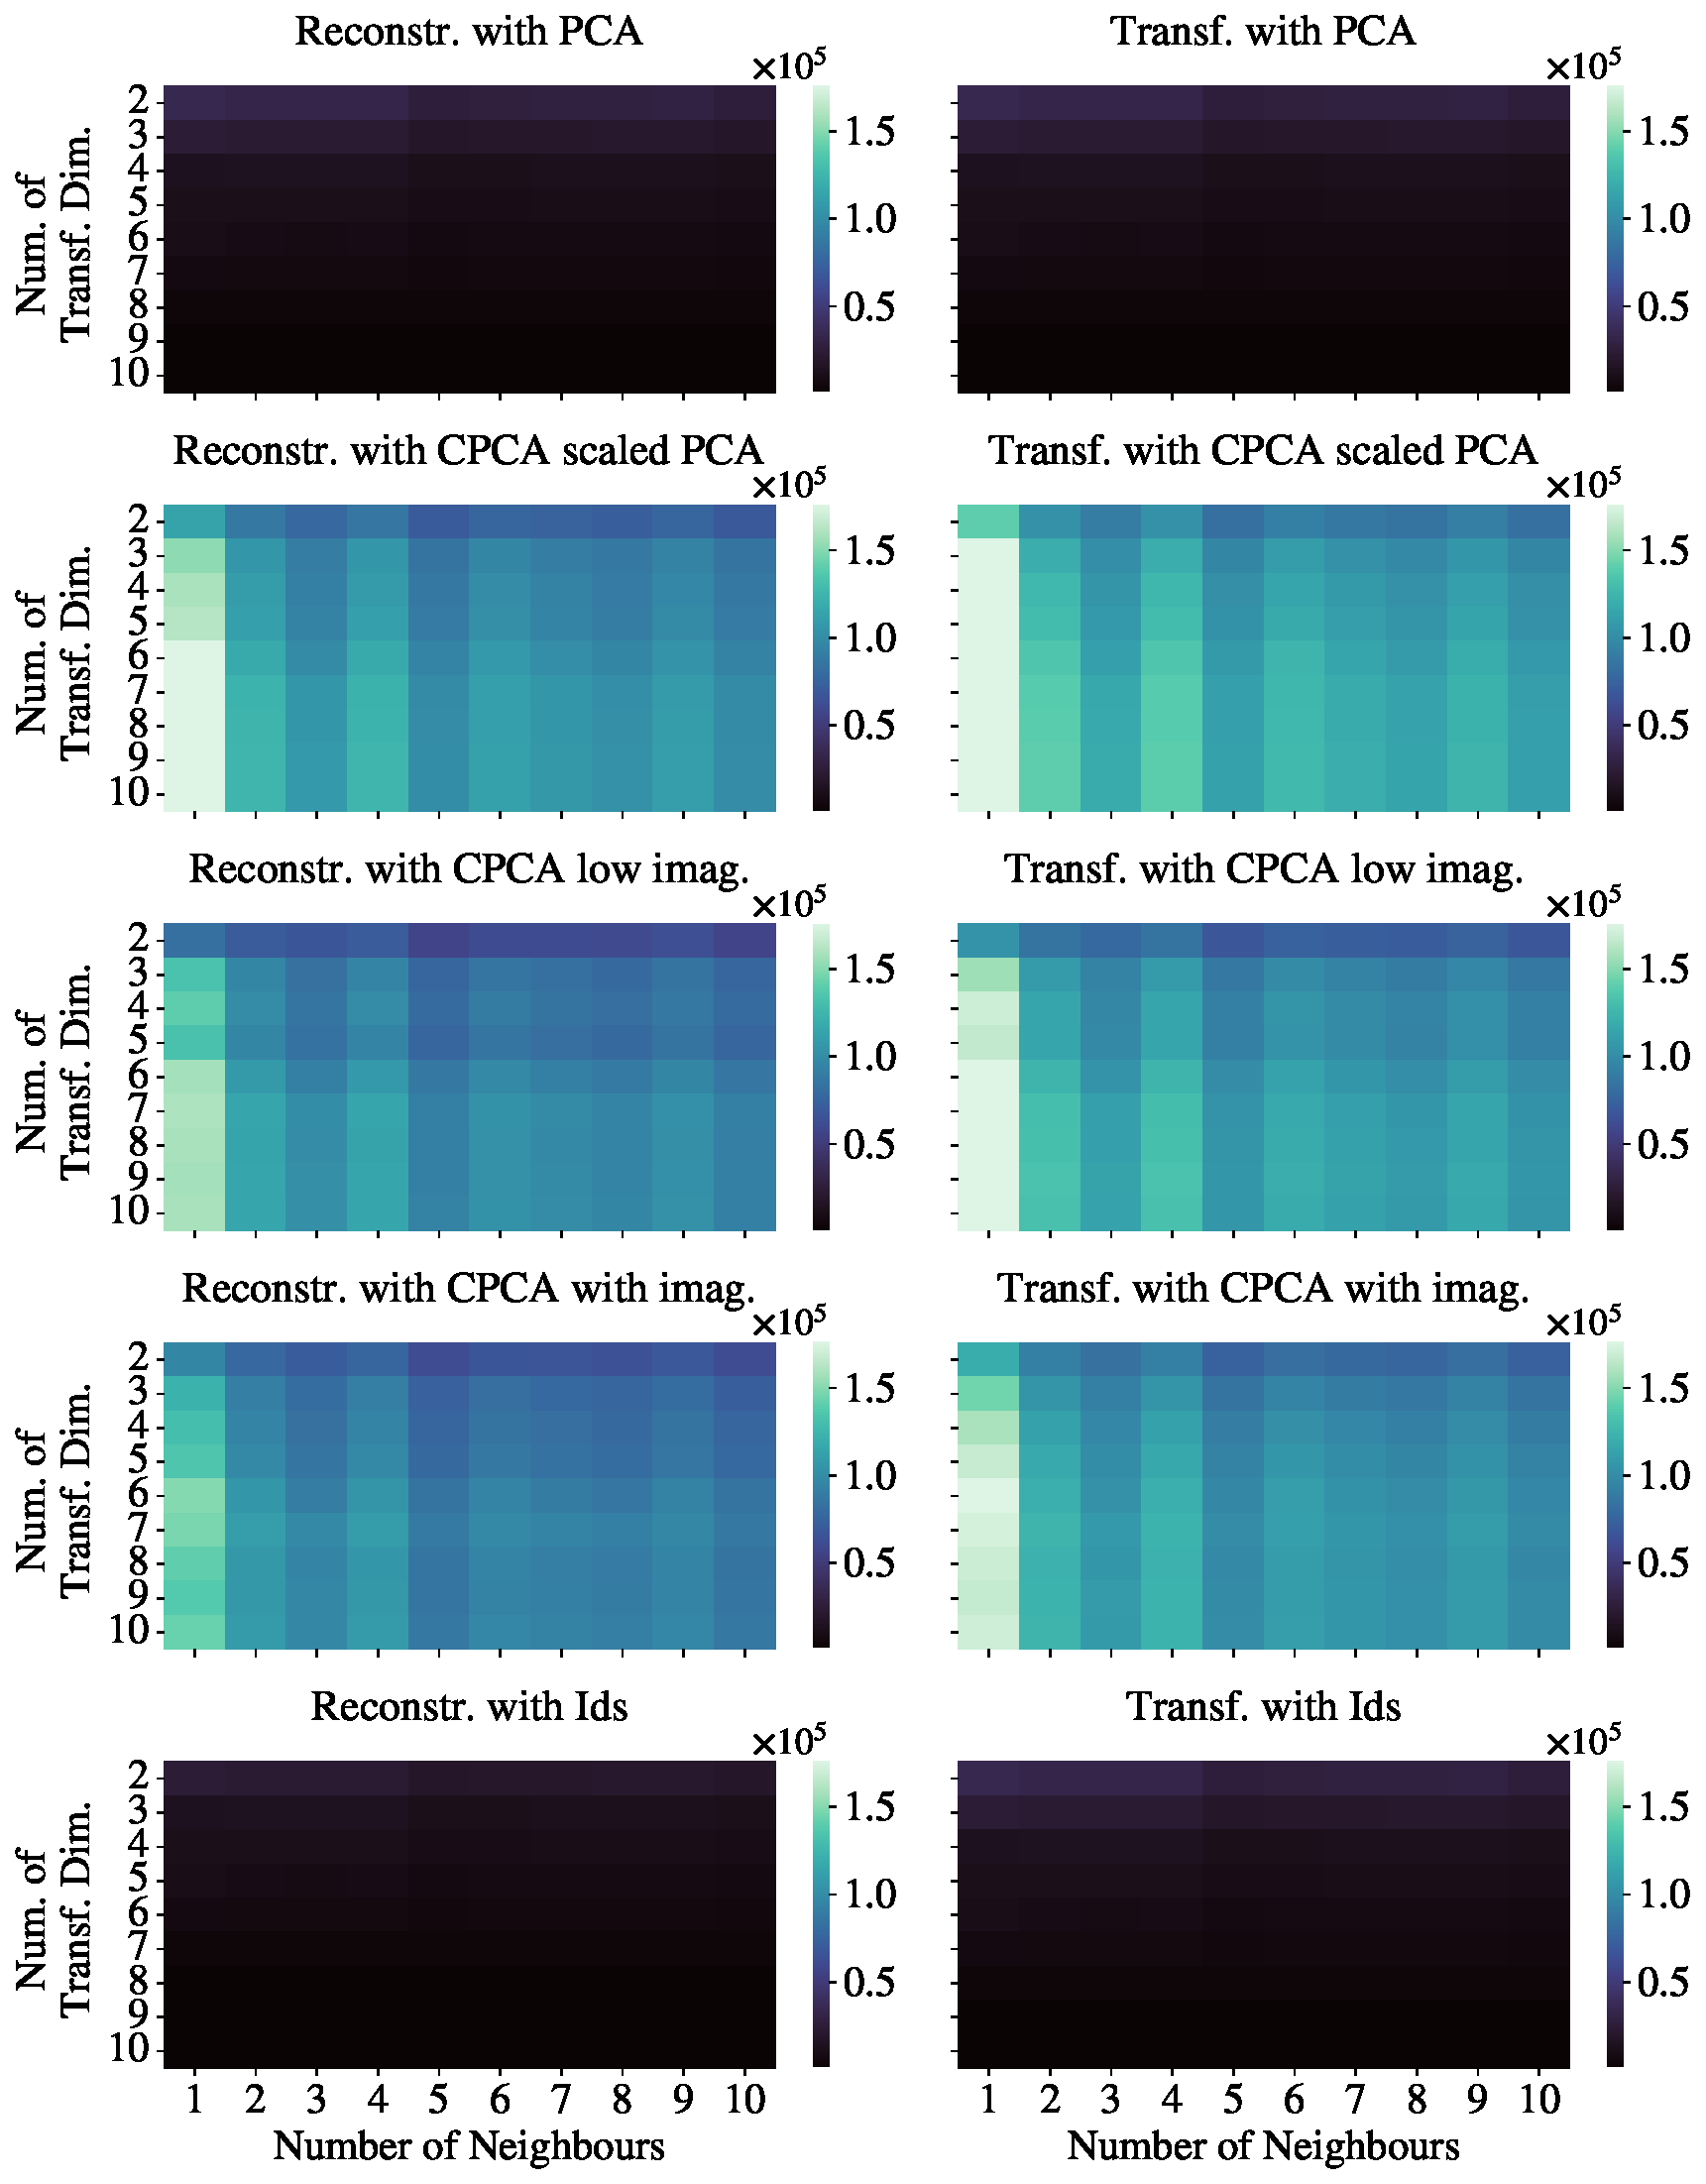
\includegraphics[width = \textwidth]{images/multiple_runs/cpca/zigzag/num_neigh_vs_dyn_low/multiple_scalar_product_10runs_5lines_100points_10neighbours.pdf}
    \caption{Multiple-Neighbour-Relations measure on zigzag data: comparing the results for increasing numbers of neighbours and dimensionality of the transformed space}\label{fig:cpca-num_neigh_vs_dyn_low-zigzag-mscal}
\end{figure}

\begin{figure}
    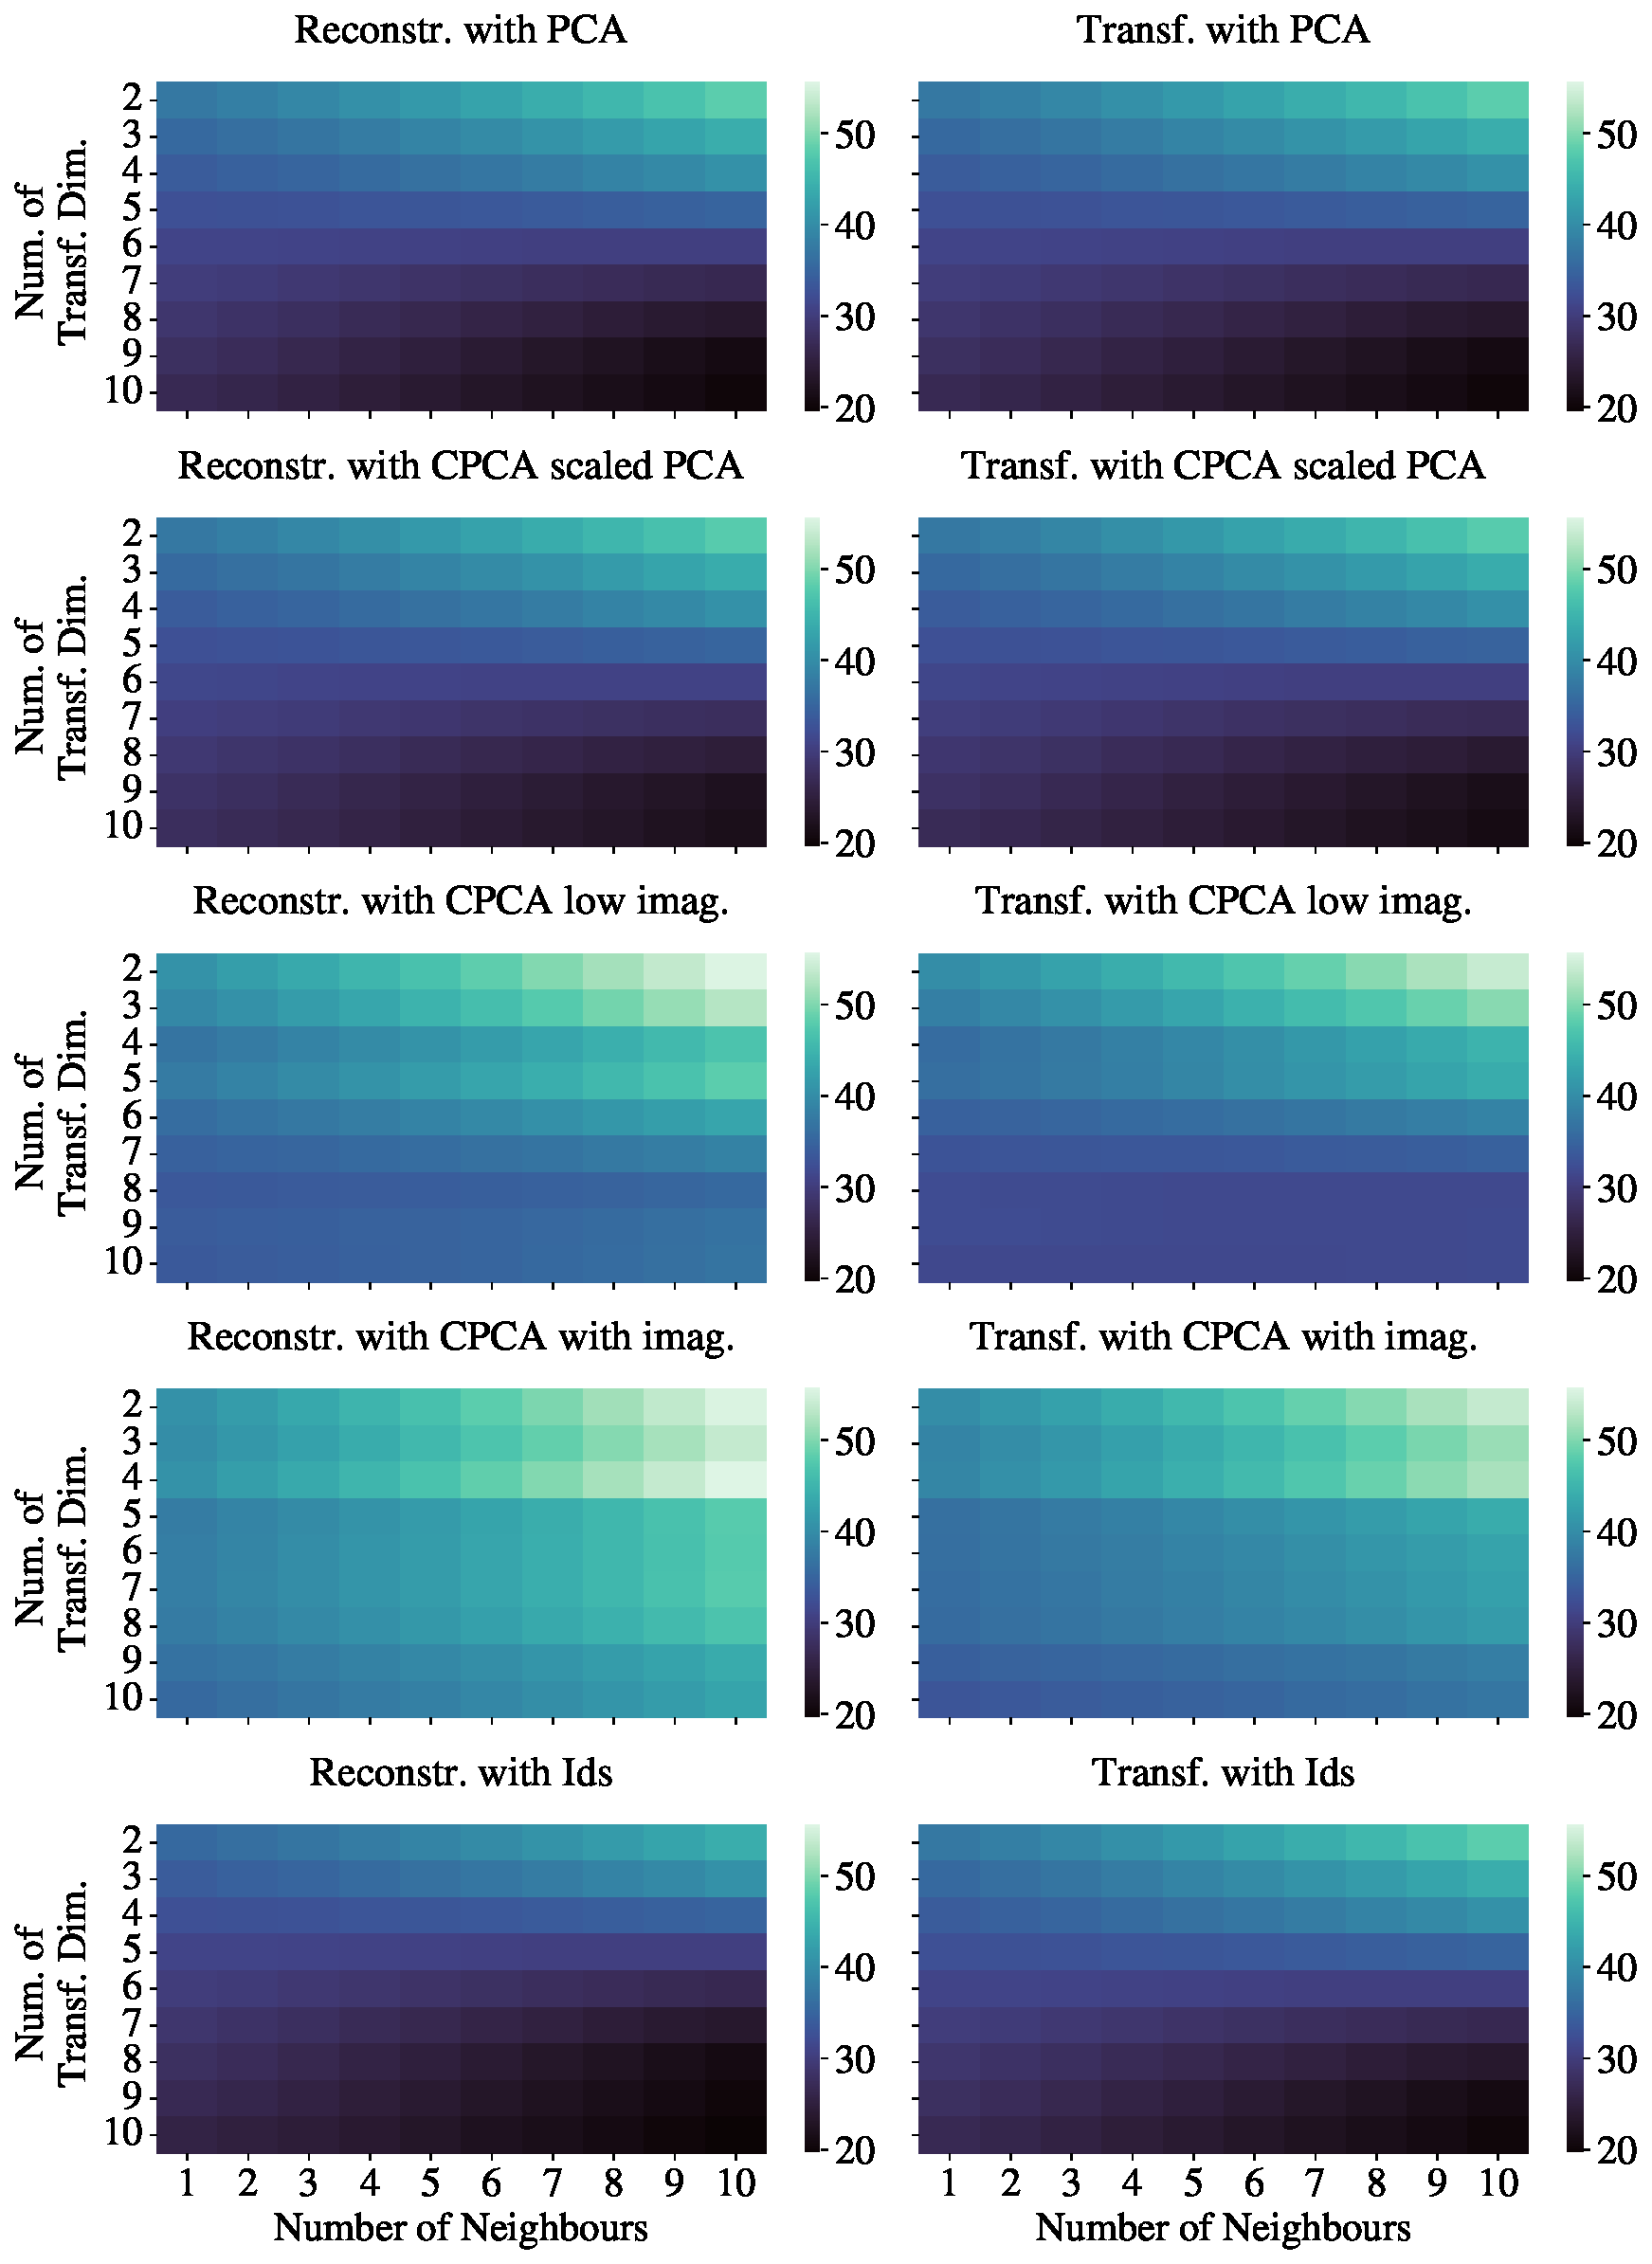
\includegraphics[width = \textwidth]{images/multiple_runs/cpca/one_line/num_neigh_vs_dyn_low/euclidean_10runs_5lines_100points_10neighbours.pdf}
    \caption{Neighbour-Distance measure on smoothly ordered data: comparing the results for increasing numbers of neighbours and dimensionality of the transformed space}\label{fig:cpca-num_neigh_vs_dyn_low-oneline-euclidean}
\end{figure}

\begin{figure}
    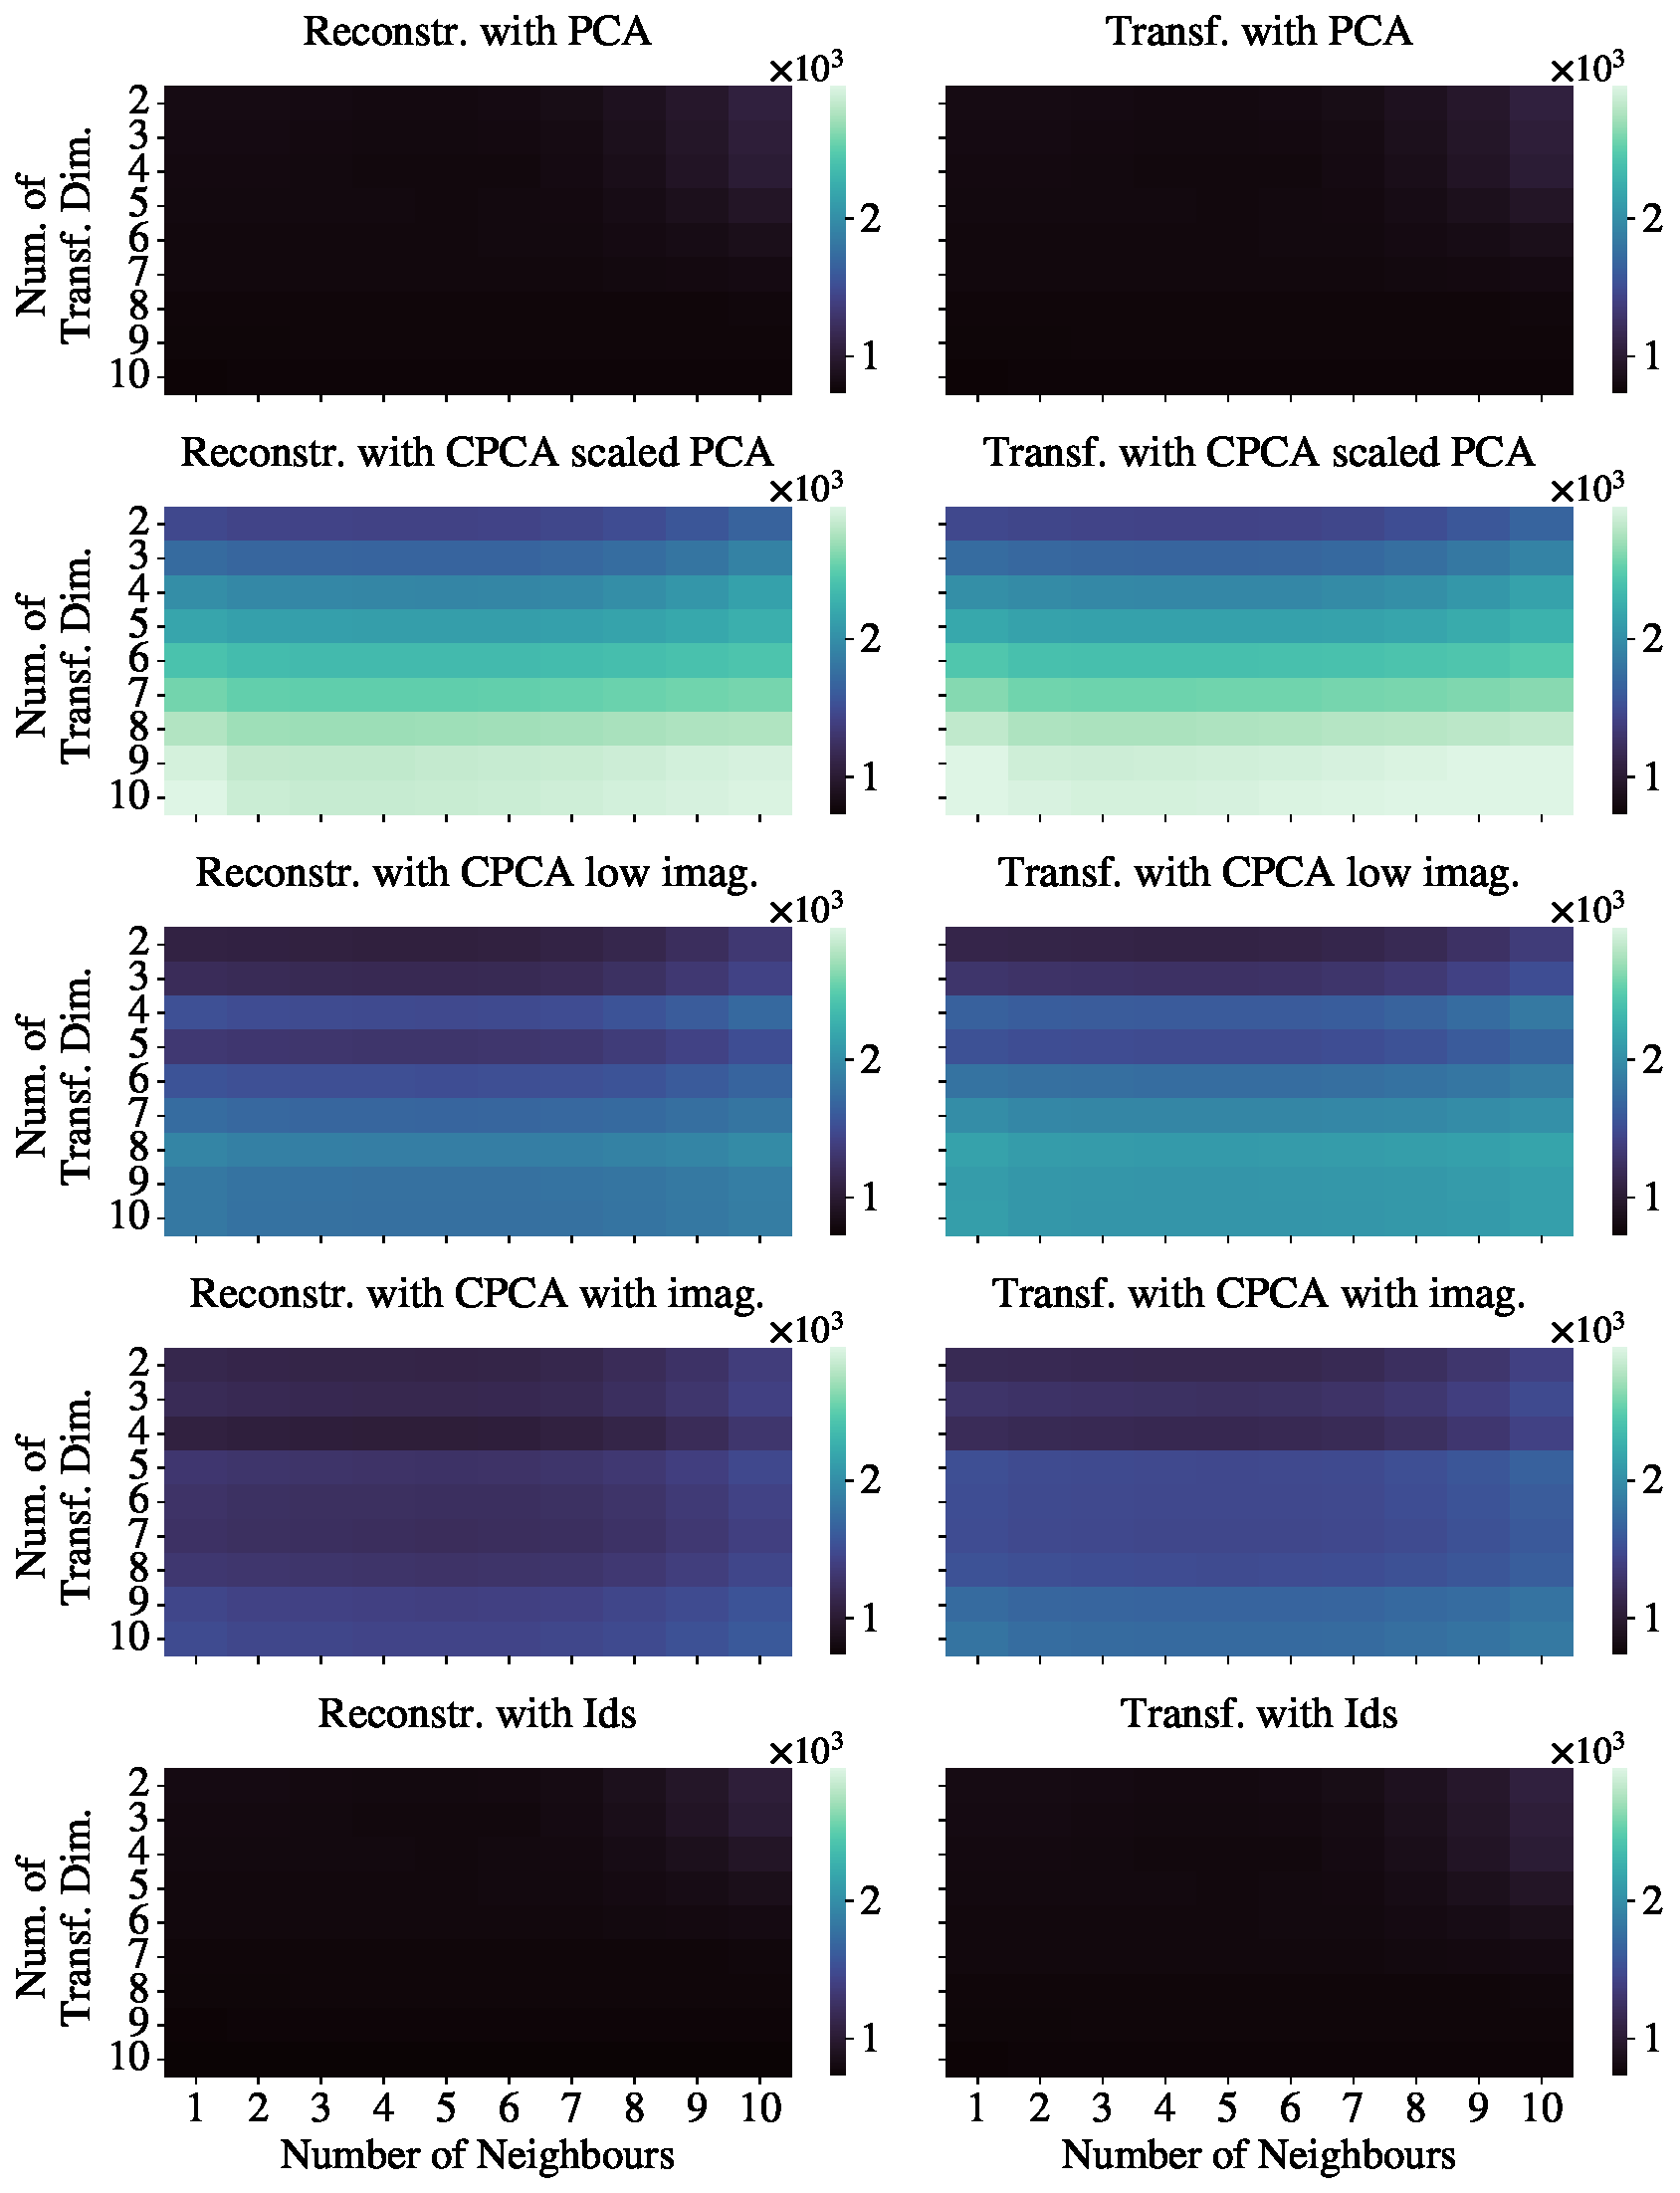
\includegraphics[width = \textwidth]{images/multiple_runs/cpca/one_line/num_neigh_vs_dyn_low/multiple_scalar_product_10runs_5lines_100points_10neighbours.pdf}
    \caption{Multiple-Neighbour-Relation measure on smoothly ordered data: comparing the results for increasing numbers of neighbours and dimensionality of the transformed space}\label{fig:cpca-num_neigh_vs_dyn_low-oneline-mscal}
\end{figure}

\begin{figure}
    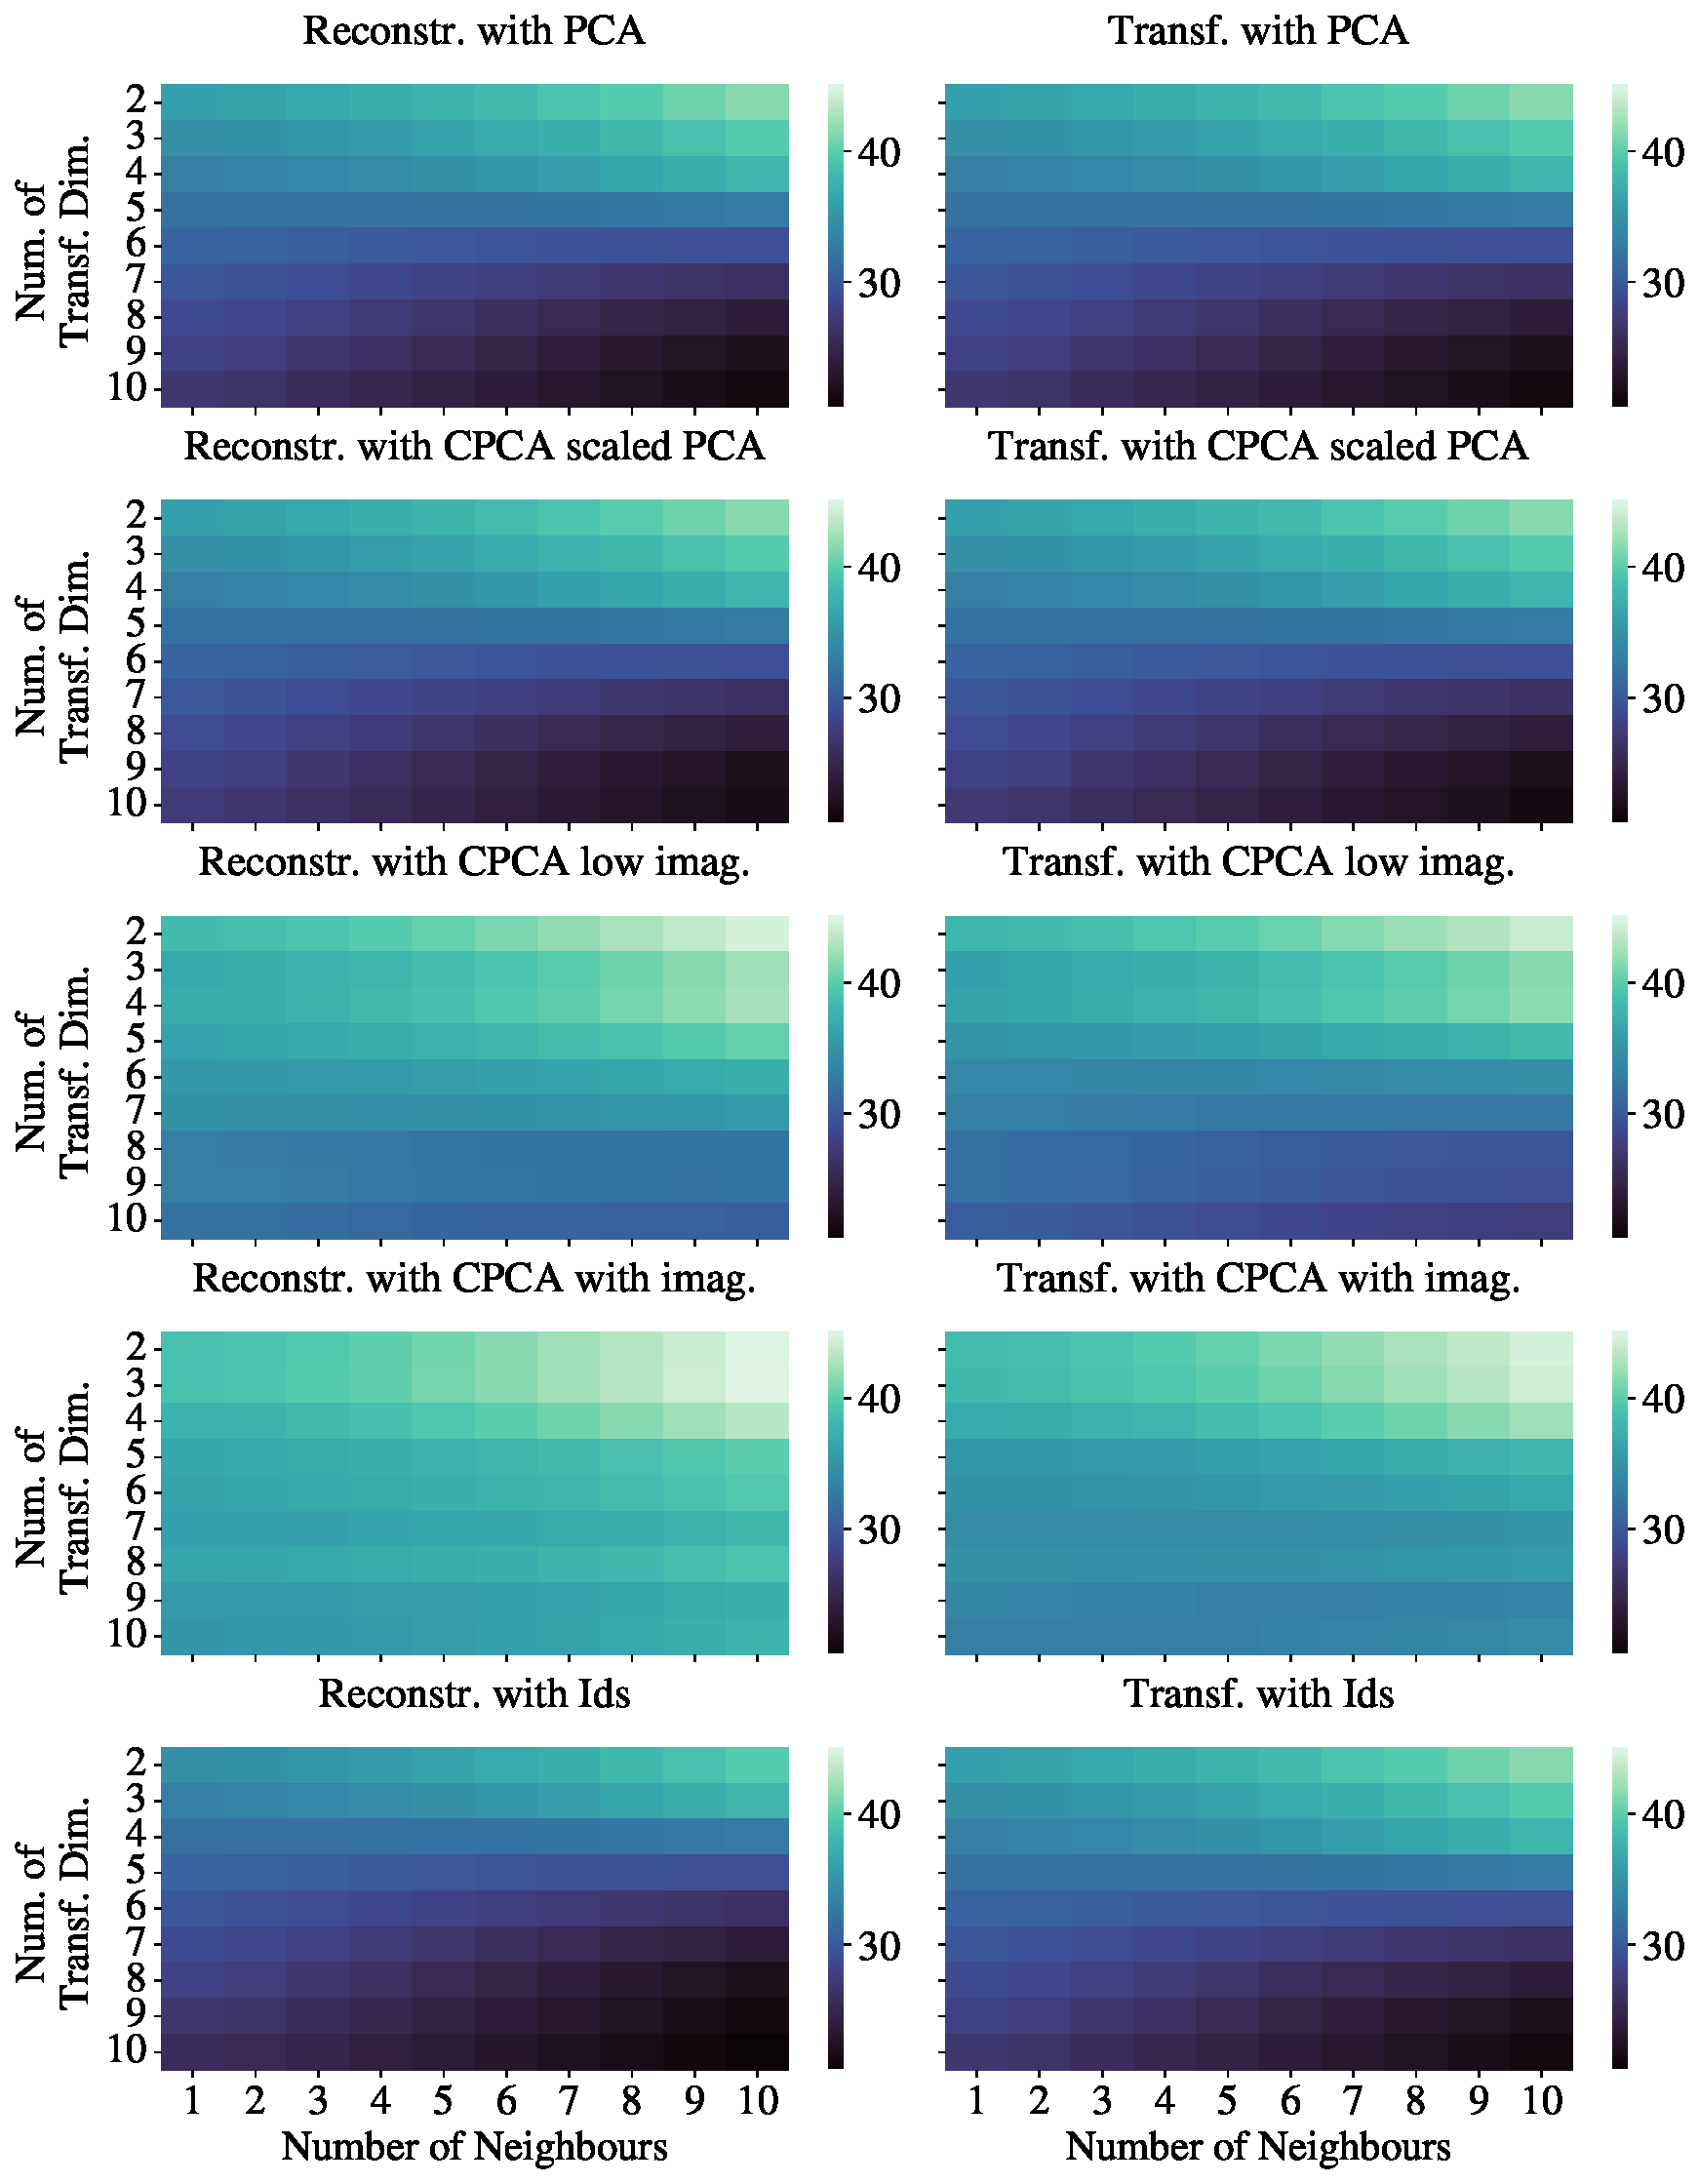
\includegraphics[width = \textwidth]{images/multiple_runs/cpca/sep_lines/num_neigh_vs_dyn_low/euclidean_10runs_5lines_100points_10neighbours.pdf}
    \caption{Neighbour-Distance measure on data on separate lines: comparing the results for increasing numbers of neighbours and dimensionality of the transformed space} \label{fig:cpca-num_neigh_vs_dyn_low-seplines-euclidean}
\end{figure}


\begin{figure}
    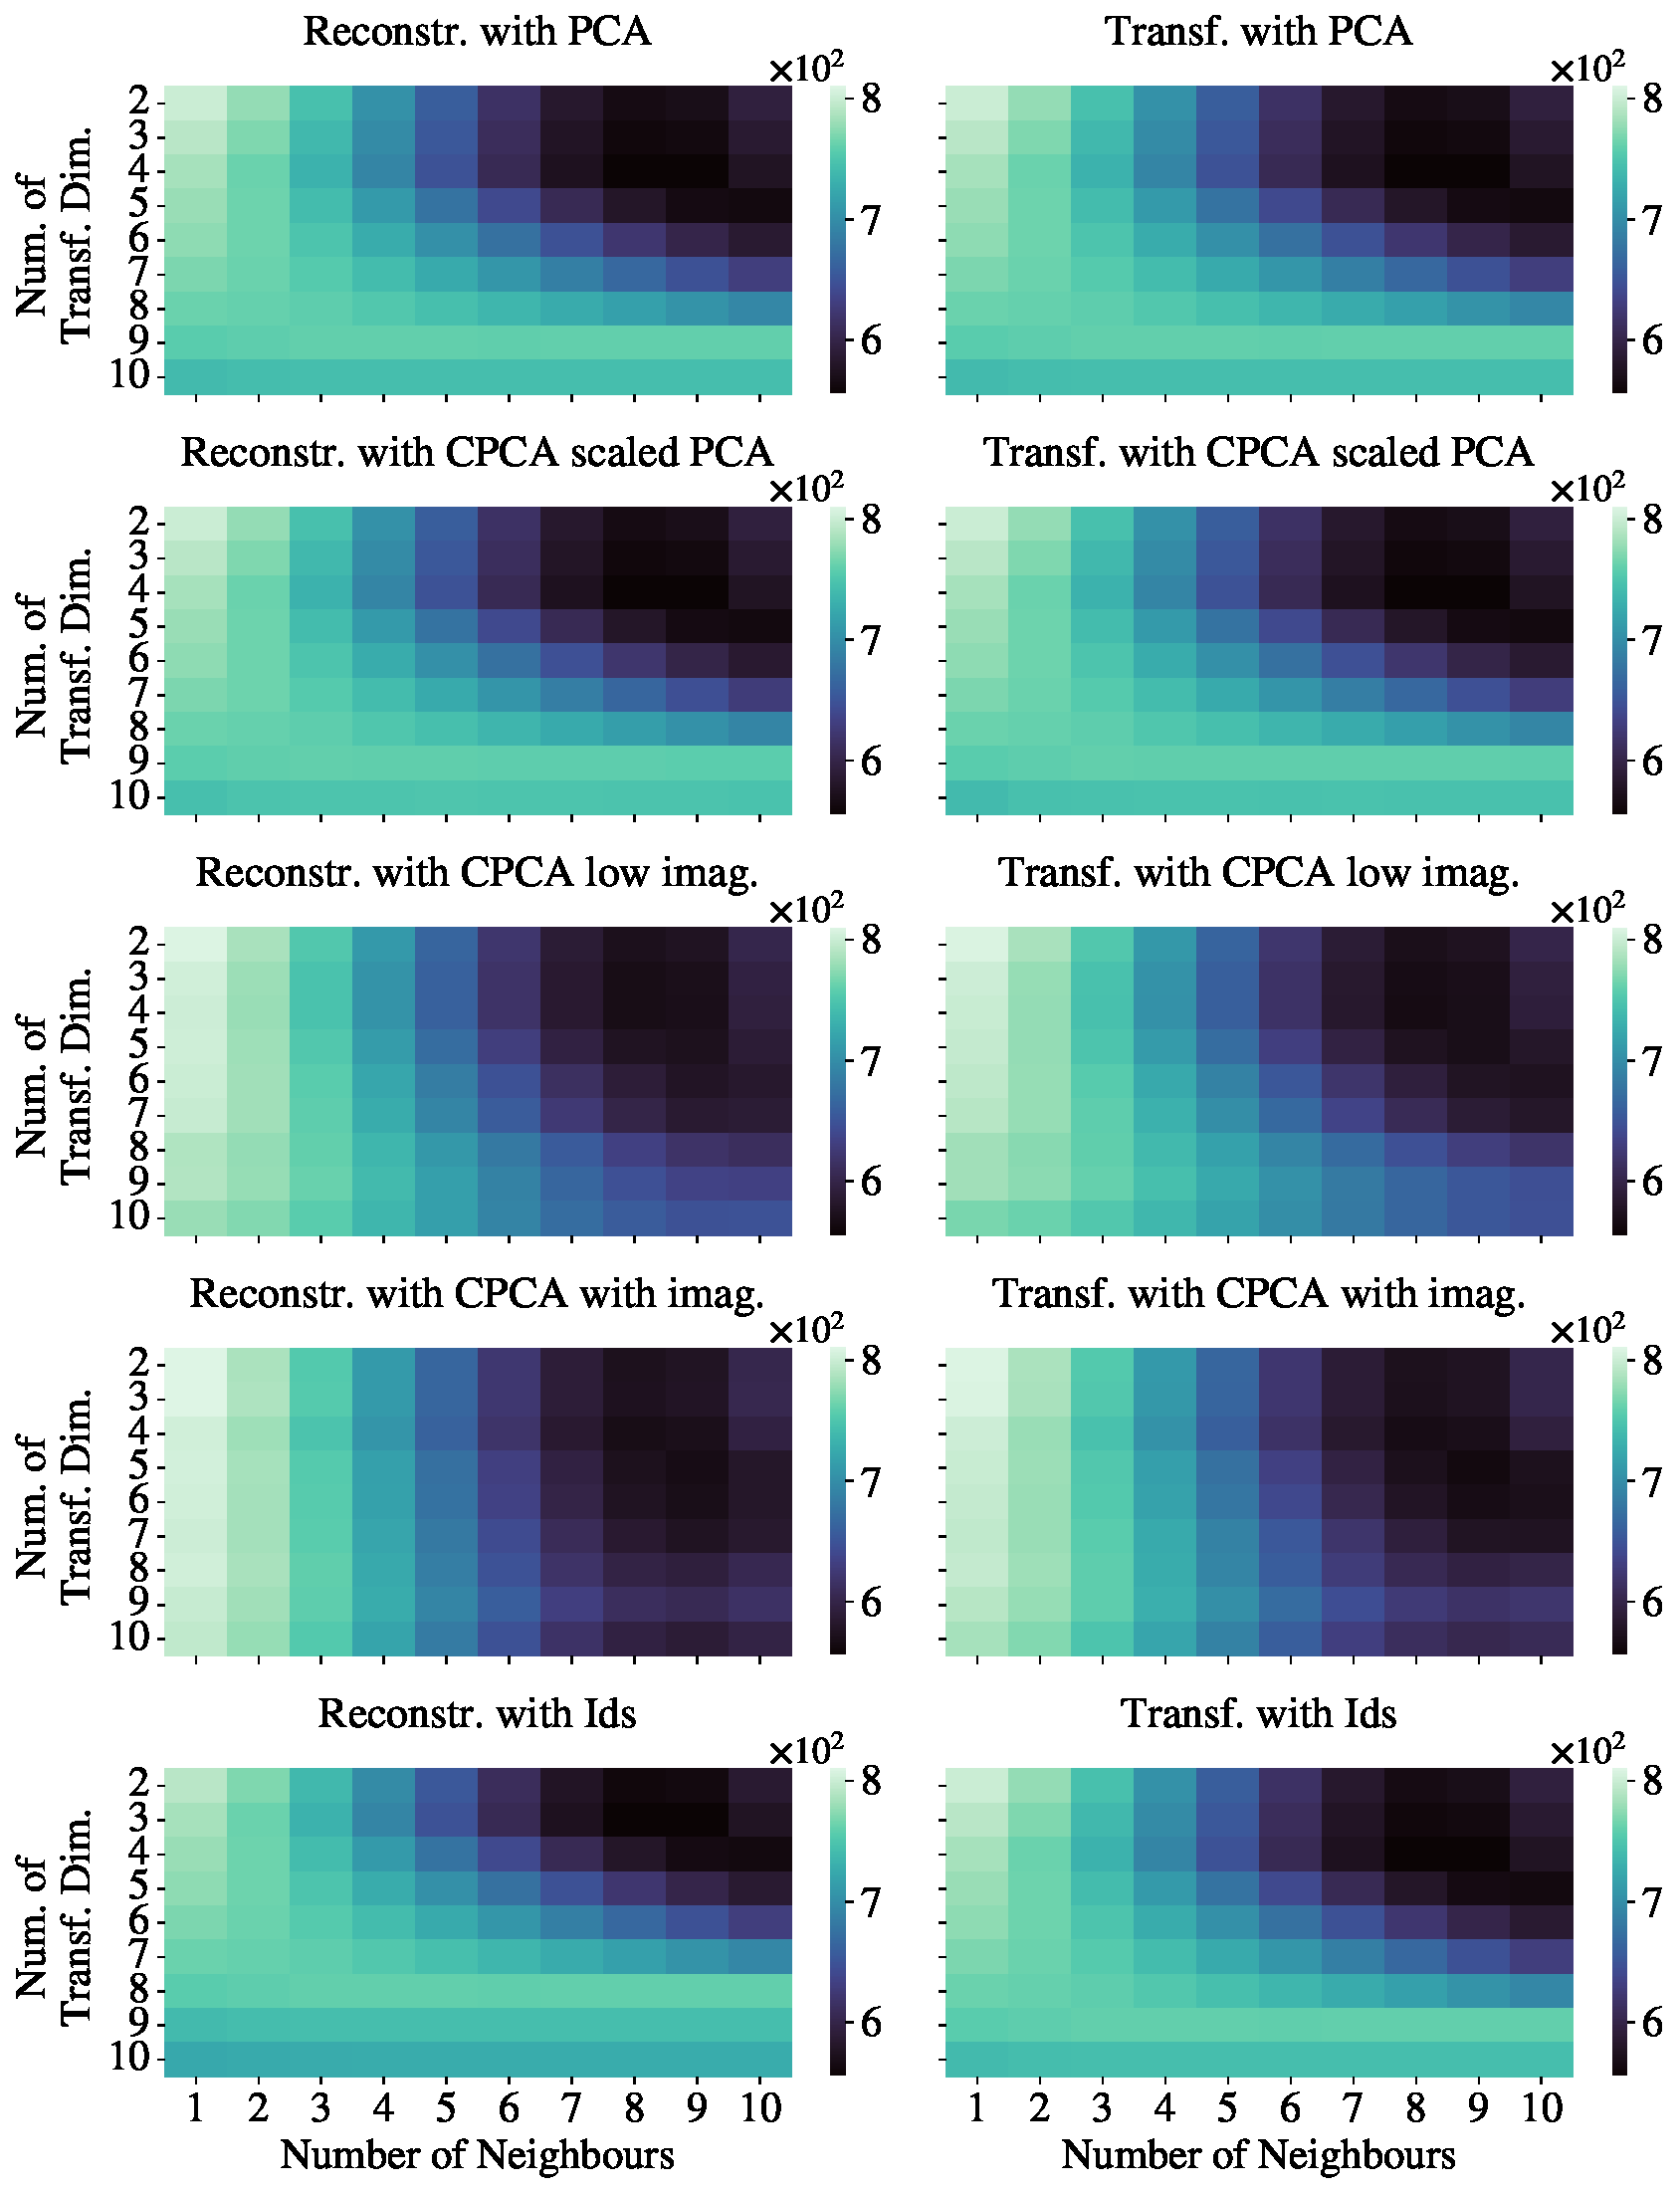
\includegraphics[width = \textwidth]{images/multiple_runs/cpca/sep_lines/num_neigh_vs_dyn_low/multiple_scalar_product_10runs_5lines_100points_10neighbours.pdf}
    \caption{Multiple-Neighbour-Relation measure on data in separate lines: comparing the results for increasing numbers of neighbours and dimensionality of the transformed space}\label{fig:cpca-num_neigh_vs_dyn_low-seplines-mscal}
\end{figure}

\FloatBarrier

\section{Evaluation with PCA* on Synthetic Data} \label{sec:evaluation-synthetic}
In this section, we directly compare PCA* with other commonly used dimensionality reduction techniques.
Based on the promising results obtained from initial experiments with PCA*, we have chosen to prioritise it as the primary dimensionality reduction method for our extended analyses.
We evaluate PCA* alongside other methods across four distinct kinds of experiments using the generated data, outlined in Section~\ref{generated_data}.

Analogously to the previous experiments, we generate 10 different datasets consisting of 5 lines, each entailing 100 data points with jitter.
These datasets strongly depend on the seed with which they are generated.
The original space resides in a 100-dimensional space unless otherwise specified.
For visibility reasons, we omit to display the variance of the Neighbour-Relation (NR) and Multiple-Neighbour-Relation (MNR) measures since it remained equally large for each observation across all experiments.
When the data is organised in separate lines, we evaluate each line individually.
In the following experiments, we present a side-by-side comparison of how well distances are preserved using the Neighbour-Distance (ND) measure and how well relationships are maintained using either the NR or MNR measure, see Definitions \ref{Neighbour-Distance-Measure} and \ref{Multiple-Neighbour-Relation-Measure}.
In every evaluation, we compare the distances and relations in both, transformed and reconstructed embeddings, with the distances and relations within the original data.

Furthermore, $k$-nearest neighbours denote in this setting, the $k$-nearest neighbours on the sequence in both directions resulting in $2k$ neighbours when using the ND measure.

\subsection{Increasing the Number of Dimensions of the Original Space} \label{subsec:avg_dev_vs_dyn_high}

We explore the average deviation between the original and transformed distances while the number of dimensions of the original higher-dimensional space increases from two onward.
Therefore, by enlarging the dimensionality of the original space, we control the complexity of the data.
Then we measure the quality of the dimensionality reduction methods applied with the quality measures described in Section~\ref{quality-measures}.
We compare the relations between each preceding and succeeding data point for each element in the dataset in the original space and to its representation for the reconstructed data and respectively its lower-dimensional embedding with different metrics.
% Therefore, for the neighbour-distance measure (ND measure), we compare the summed distances to the preceding and succeeding data points on the order for all elements in the data and hence assume $k = 2$.
\begin{figure}[!htb]
    \subfigure[Neighbour-Distance Measure]{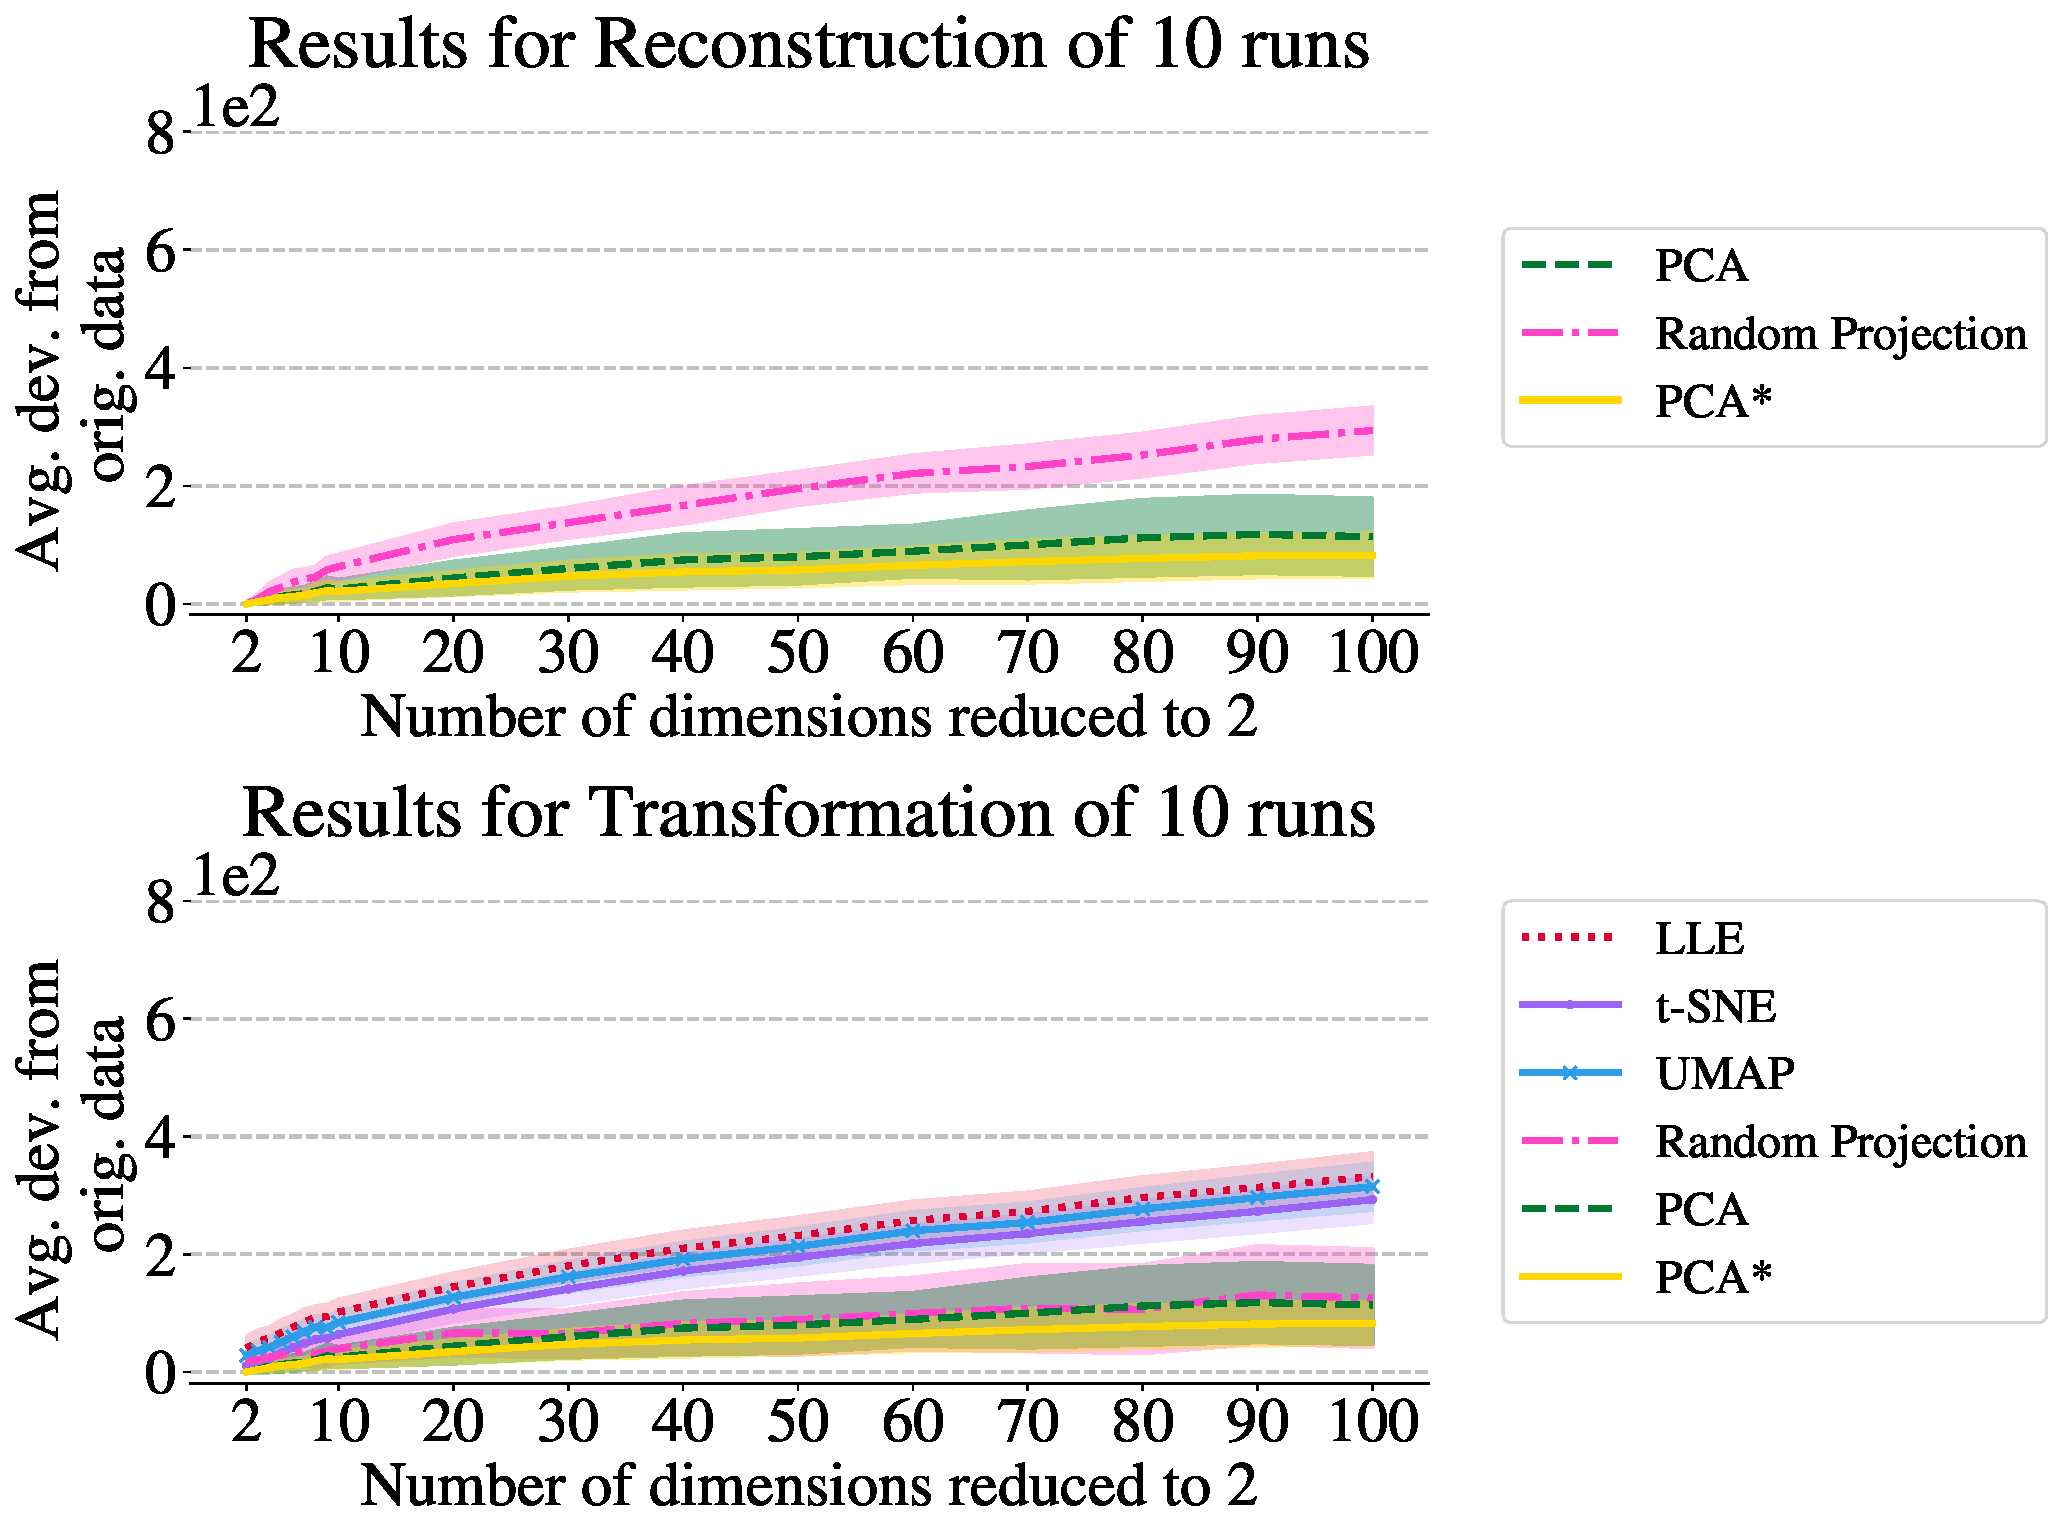
\includegraphics[width=7cm]{./images/multiple_runs/zigzag/avg_dev_vs_dyn_high/5lines_100points_1neighbours_euclidean.pdf}}
    \subfigure[Neighbour-Relation Measure]{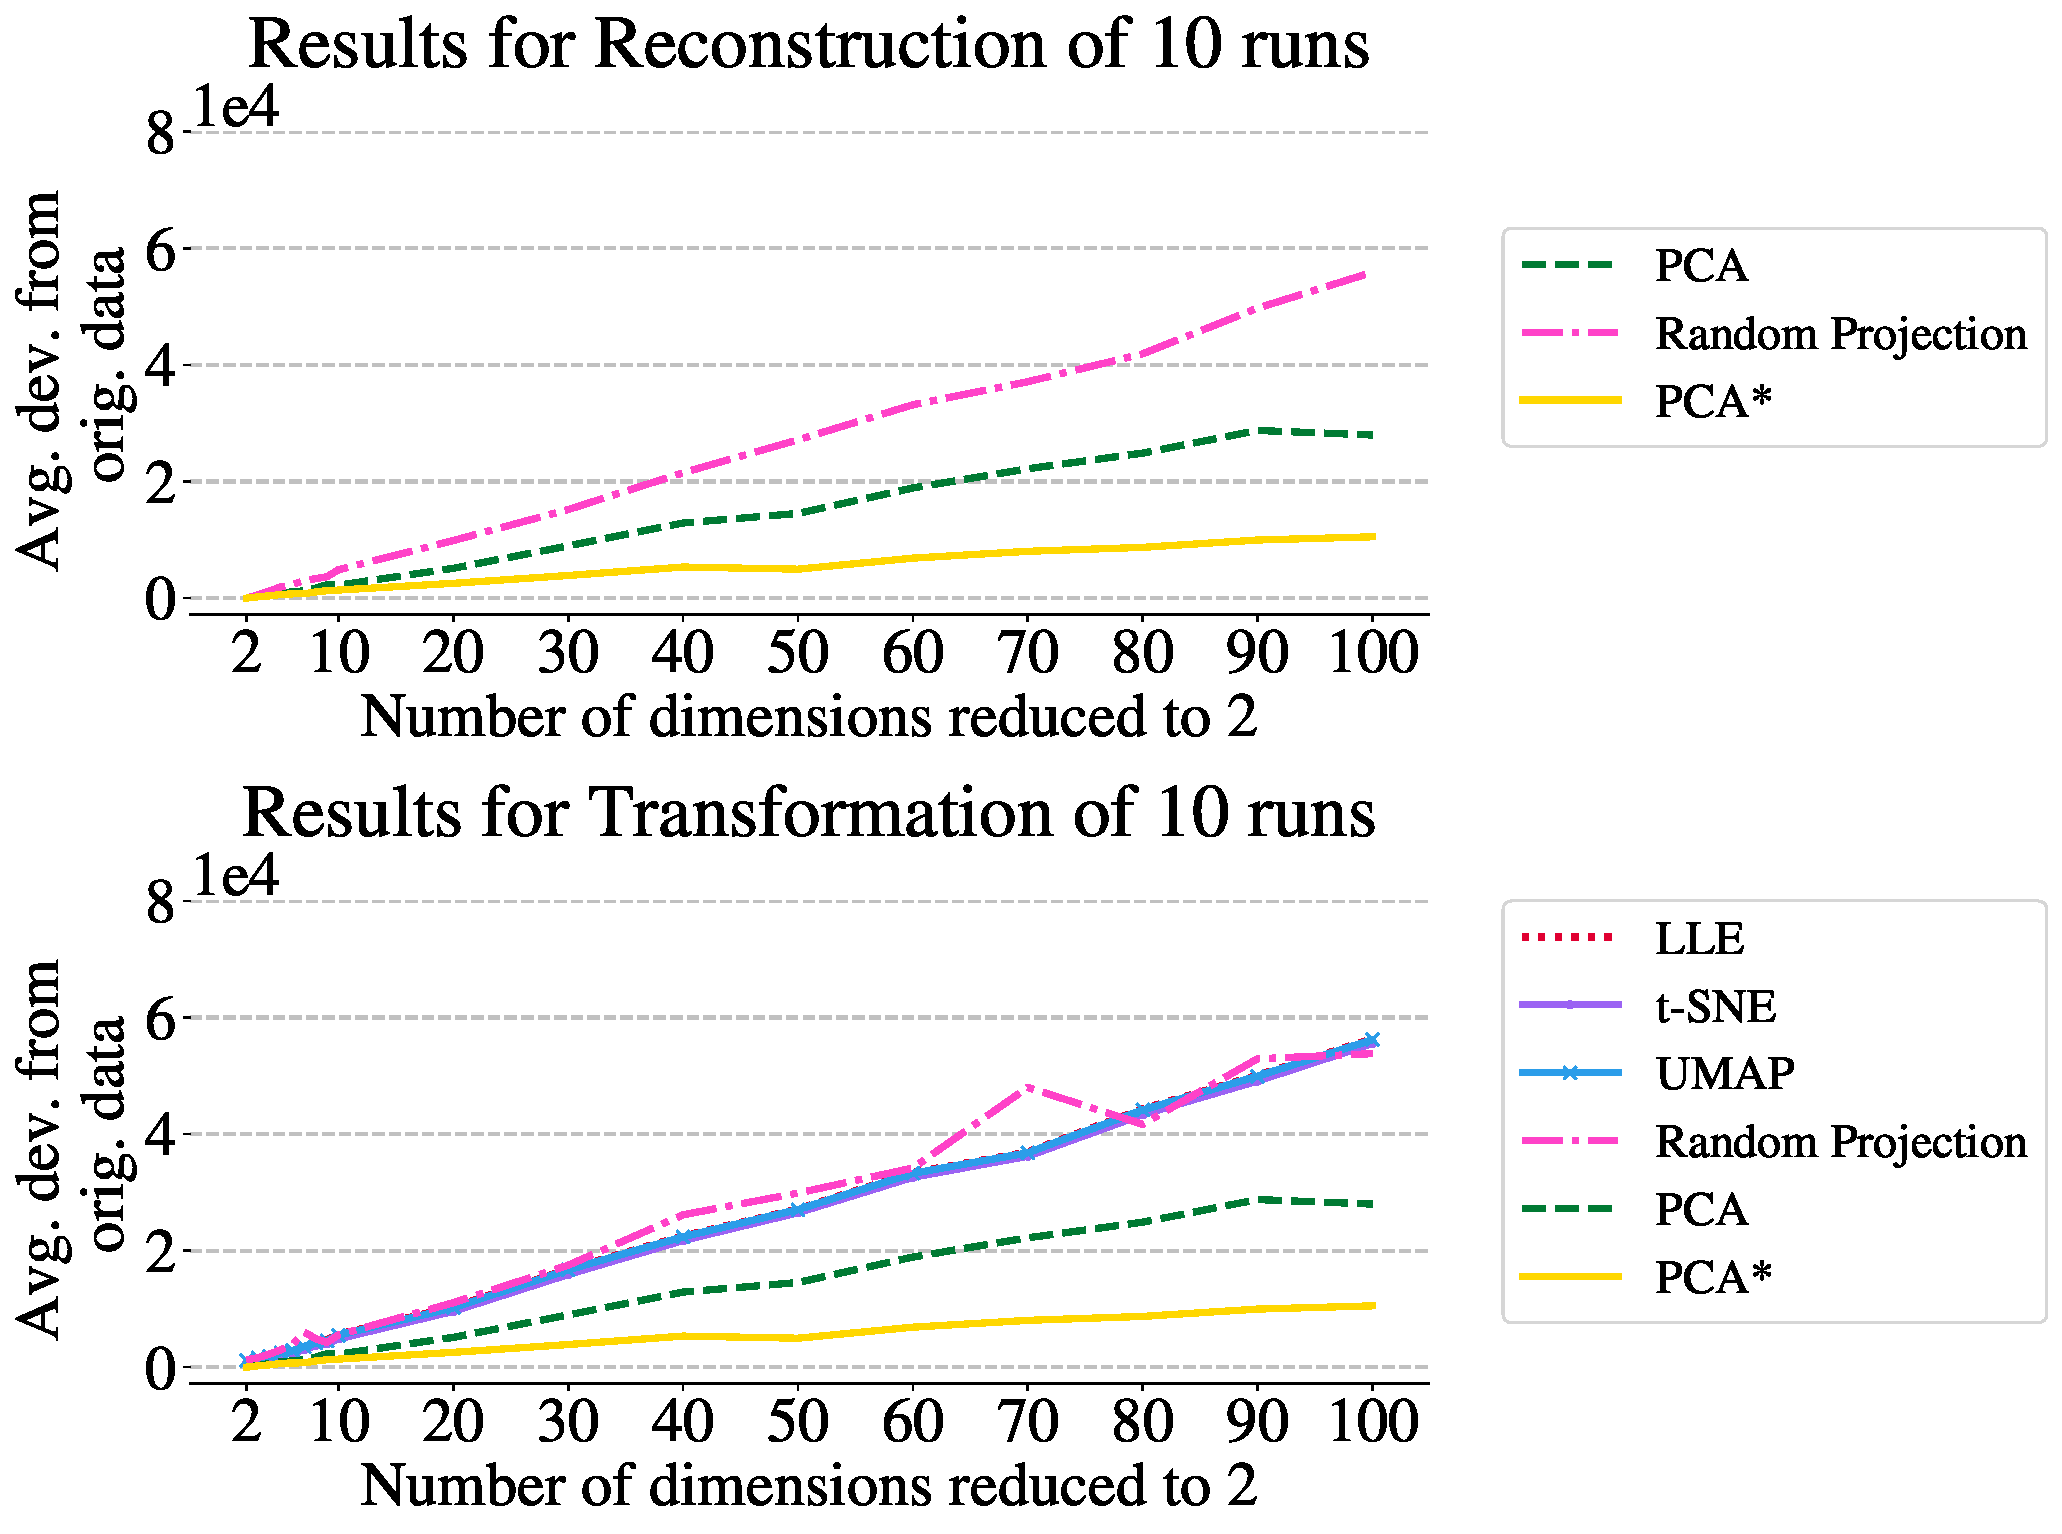
\includegraphics[width=7cm]{./images/multiple_runs/zigzag/avg_dev_vs_dyn_high/5lines_100points_1neighbours_scalar_product.pdf}}
    \caption{Results zigzag data: increasing the number of dimensions of the original data}\label{fig:avg_dev_vs_high_dim-zigzag}
\end{figure}

Figure \ref{fig:avg_dev_vs_high_dim-zigzag} presents the outcomes of dimensionality reduction methods applied to zigzag data.
Notably, PCA* stands out by preserving both distance and relations with respect to its first neighbours on the sequence more effectively than other methods, as evidenced by its lower results for both measures.
In contrast, random projection lags behind PCA and PCA* and is similar to LLE, t-SNE and UMAP.
LLE, t-SNE, and UMAP exhibit comparable results

\begin{figure}[!htb]
    \subfigure[Neighbour-Distance Measure]{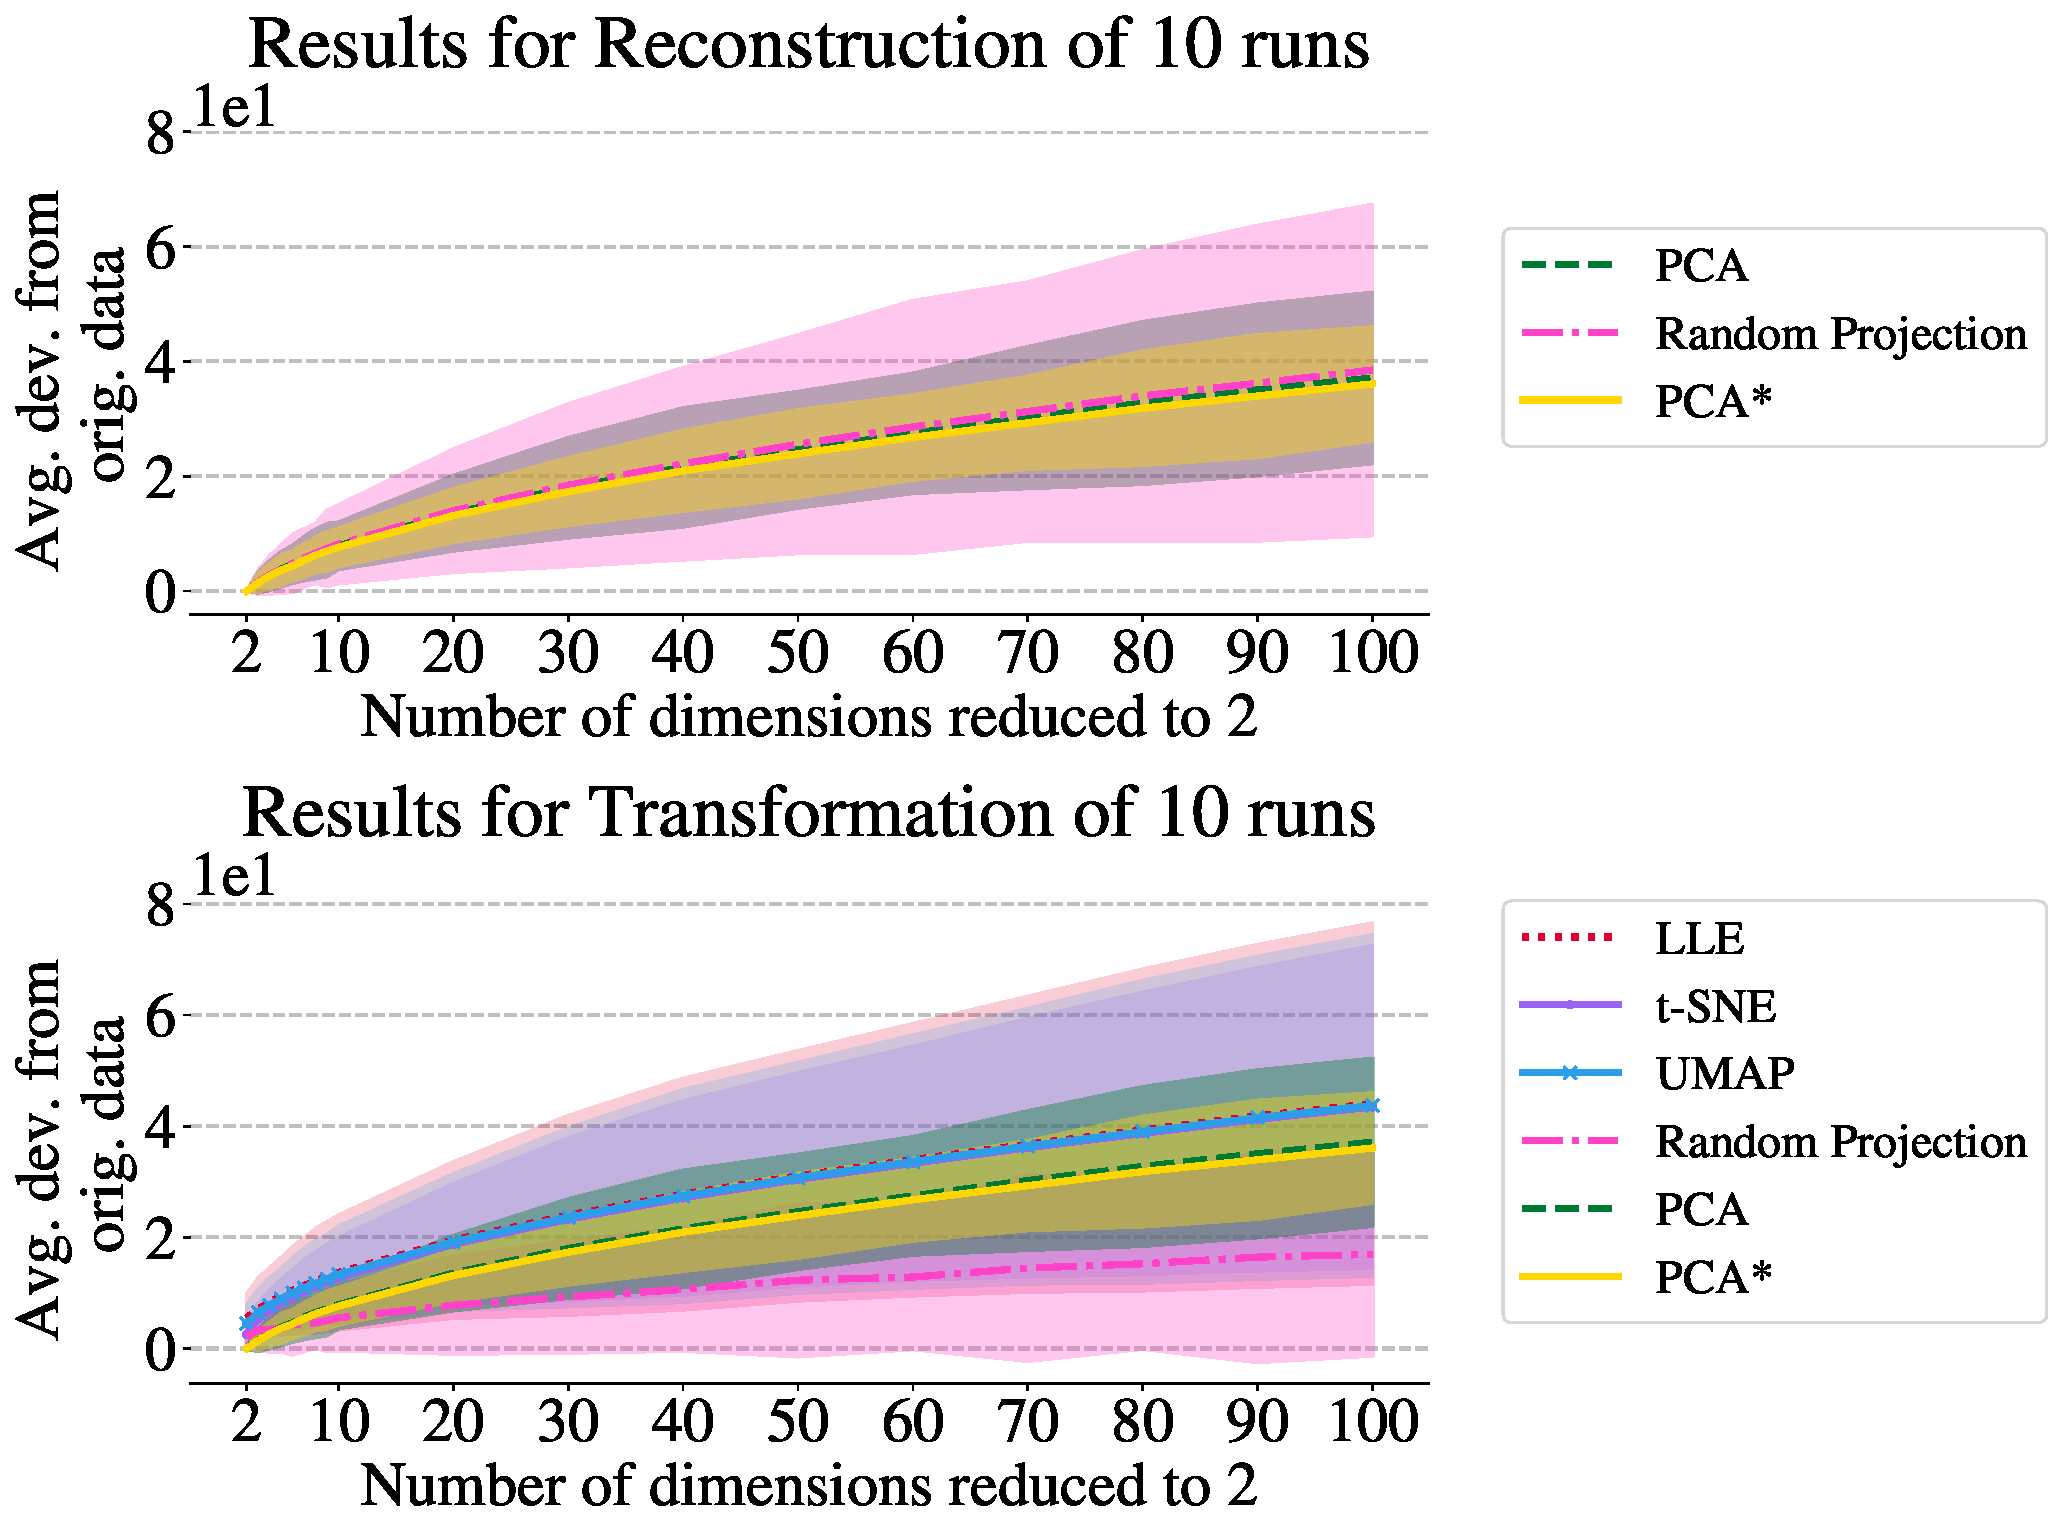
\includegraphics[width=7cm]{./images/multiple_runs/one_line/avg_dev_vs_dyn_high/5lines_100points_1neighbours_euclidean.pdf}}
    \subfigure[Neighbour-Relation Measure]{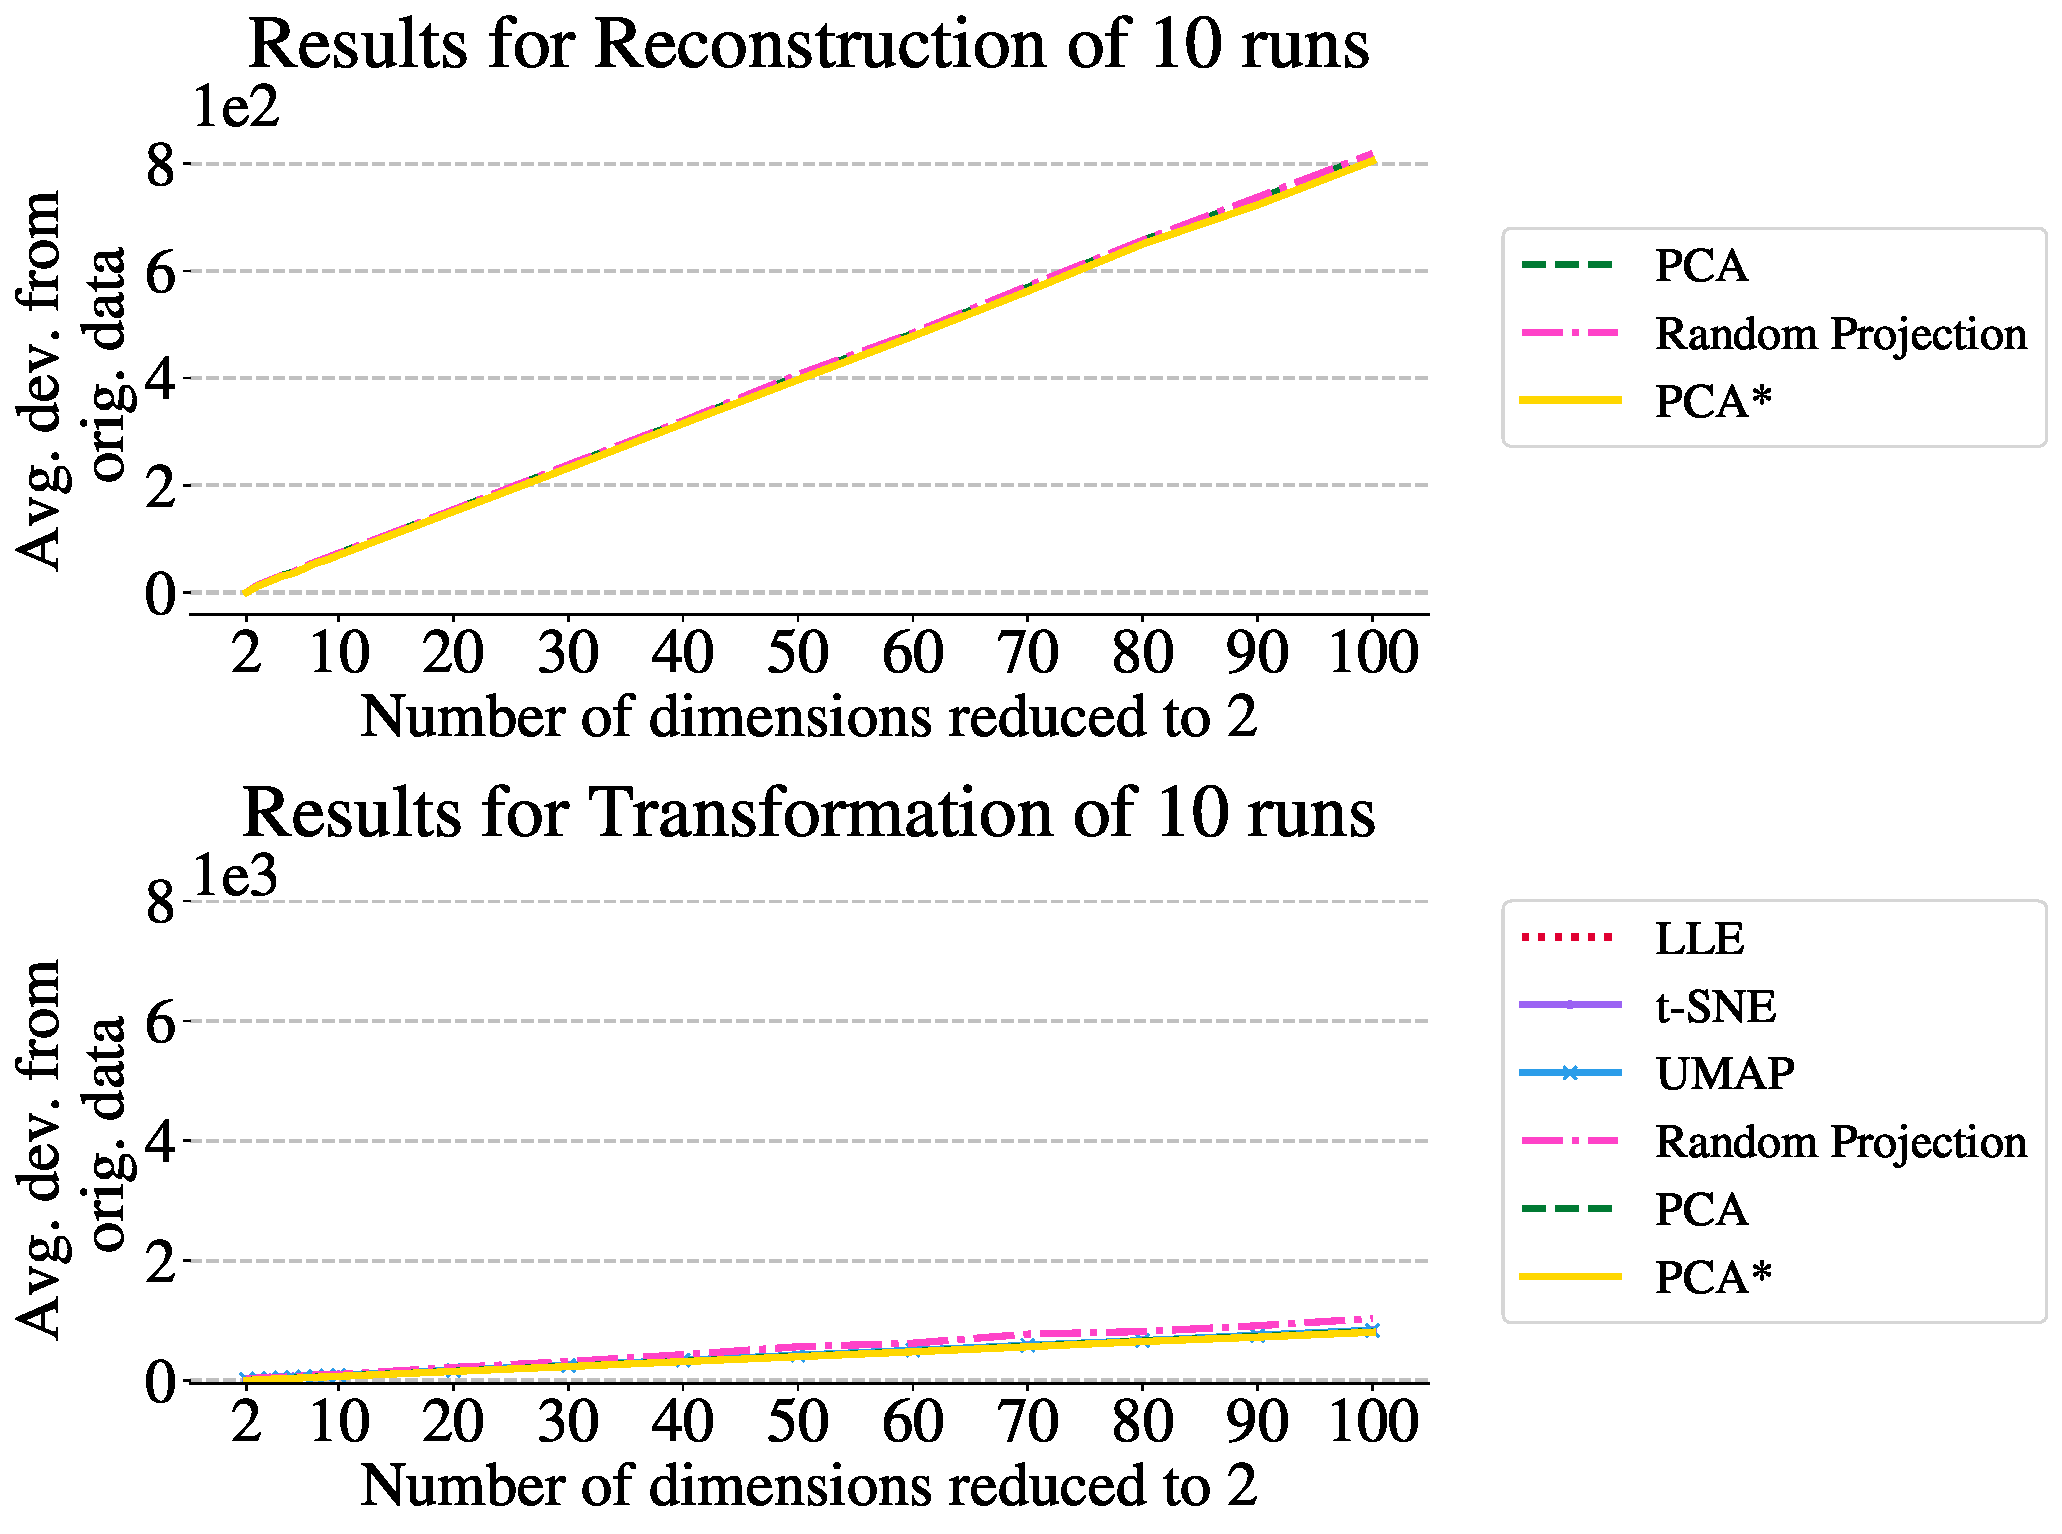
\includegraphics[width=7cm]{./images/multiple_runs/one_line/avg_dev_vs_dyn_high/5lines_100points_1neighbours_multiple_scalar_product.pdf}}
    \caption{Results for smoothly-ordered data: increasing the number of dimensions of the original data}\label{fig:avg_dev_vs_high_dim-oneline}
\end{figure}

Comparing these results to the outcomes of dimensionality reduction methods applied to data connected by a smooth line, we see that PCA* yields a mean result similar to PCA but with lower variance, as illustrated in Figure~\ref{fig:avg_dev_vs_high_dim-oneline}.
Interestingly, random projection performs well in the lower-dimensional representation, as measured with the ND measure.
This is because random projection falls under the category of local structure-preserving dimensionality reduction techniques, and when the data consists of roughly straight lines, the local structure aligns with the order-based distances.
However, it is worth noting that due to its random nature, random projection exhibits significantly higher variance than PCA*.
When assessing its results with the NR measure, it becomes evident that random projection does not preserve angular relations as effectively as PCA*, LLE, and other methods in the lower-dimensional space.
Overall all methods keep the order-based relations similarly well.

\begin{figure}[!htb]
    \subfigure[Neighbour-Distance Measure]{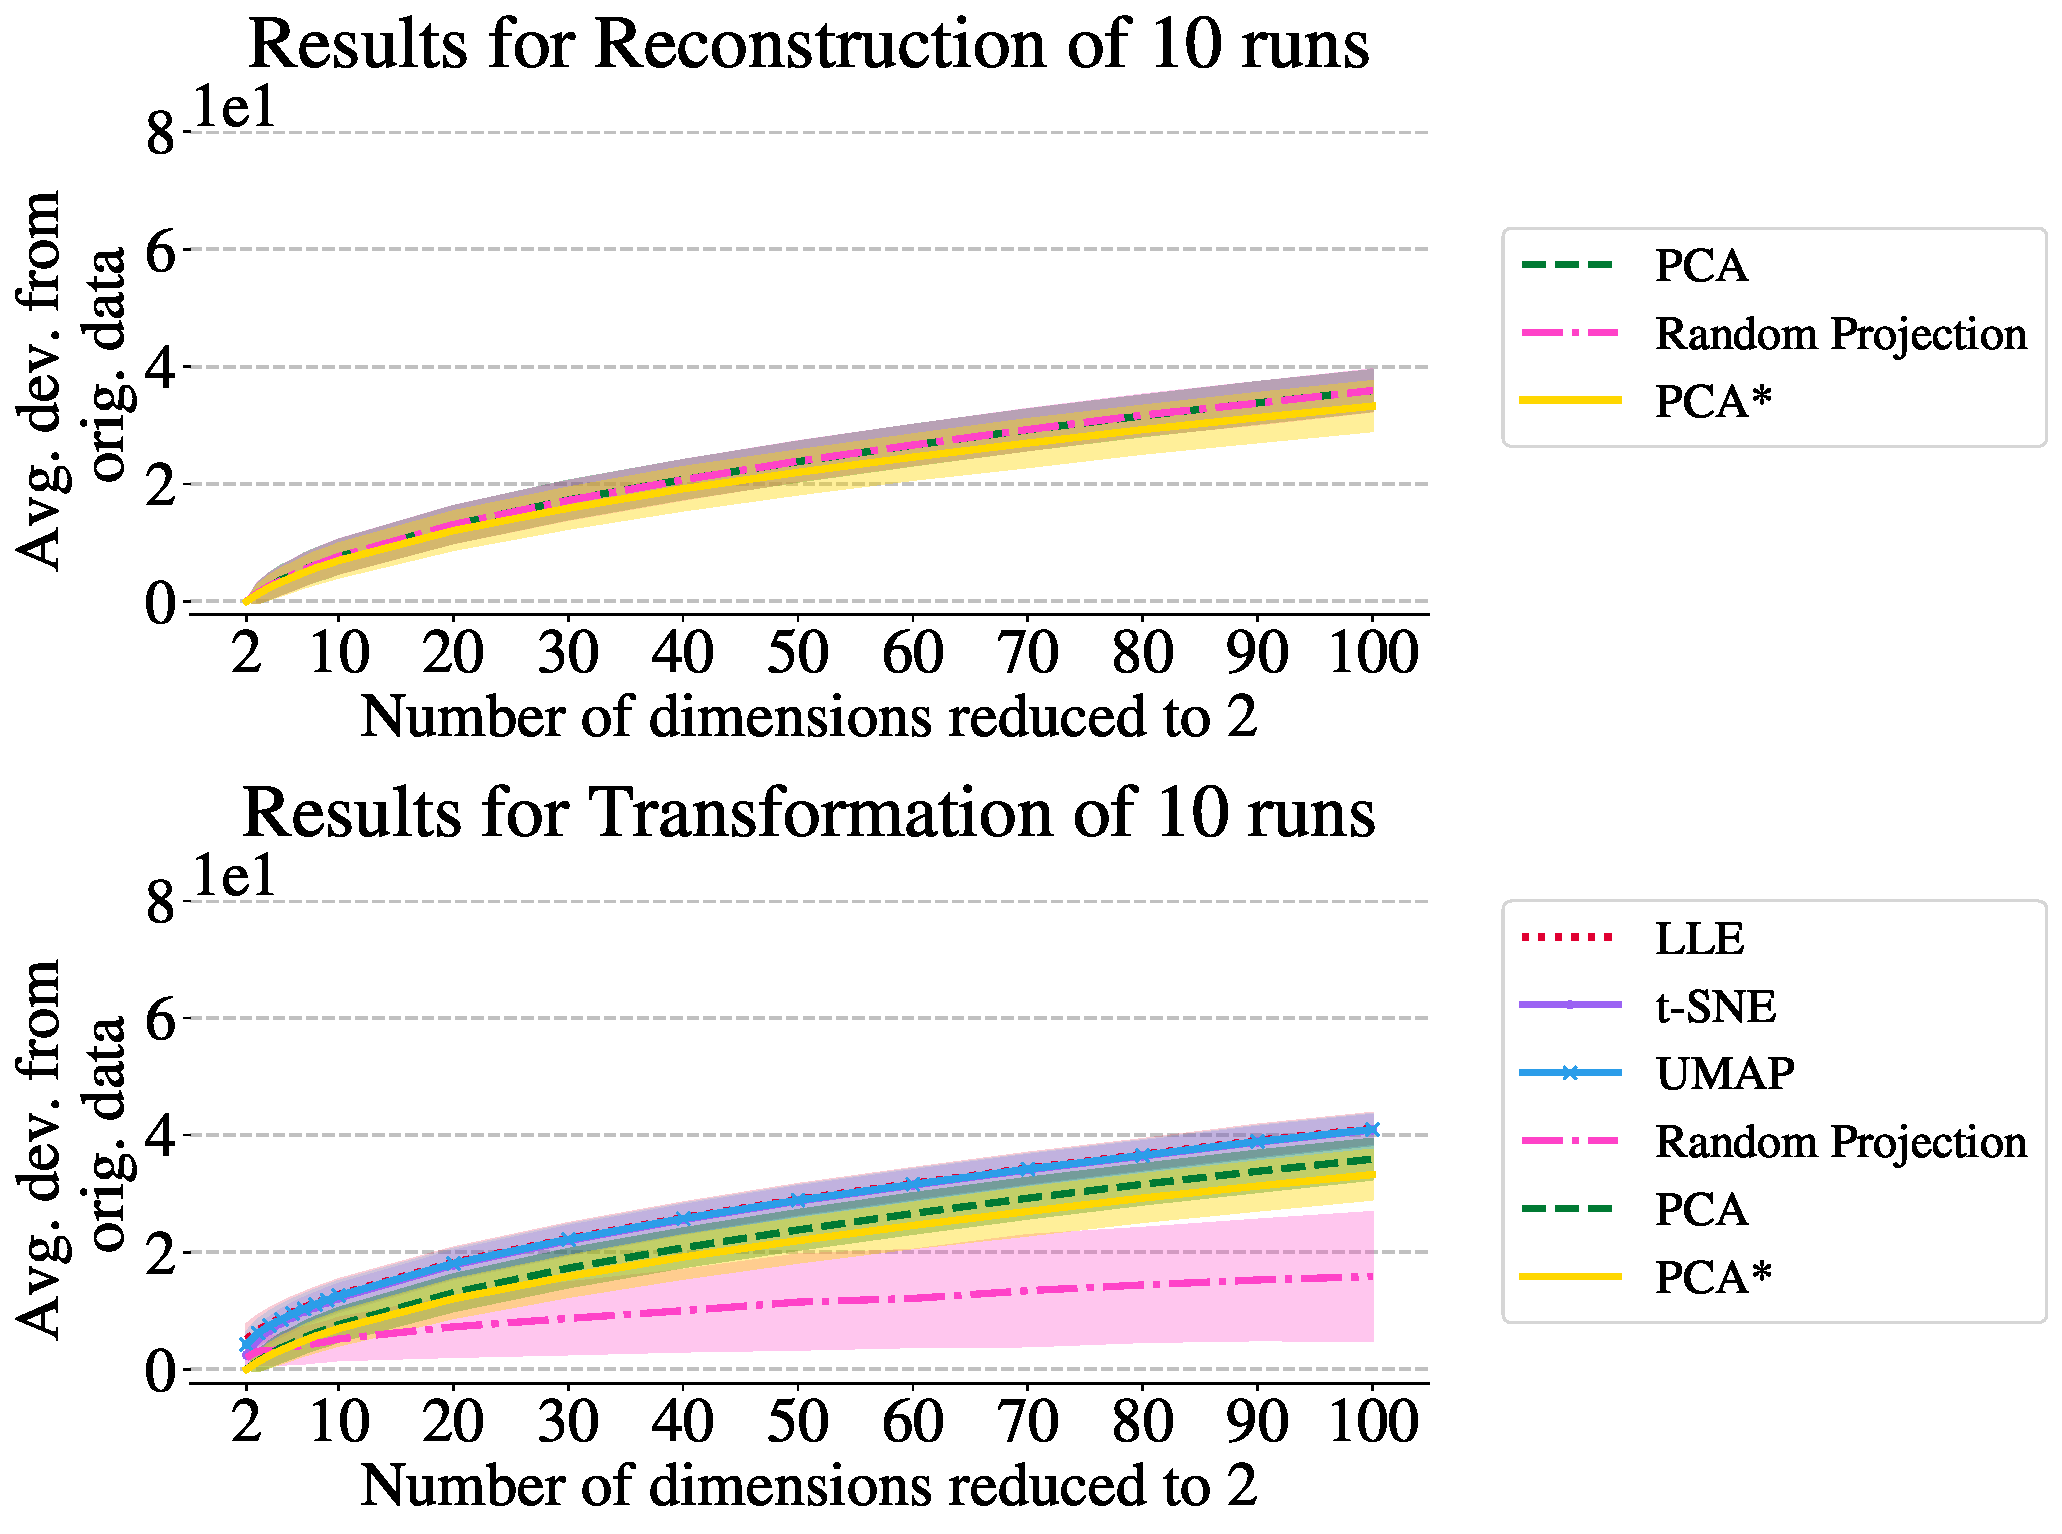
\includegraphics[width=7cm]{./images/multiple_runs/sep_lines/avg_dev_vs_dyn_high/5lines_100points_1neighbours_euclidean.pdf}}
    \hfill
    \subfigure[Neighbour-Relation Measure]{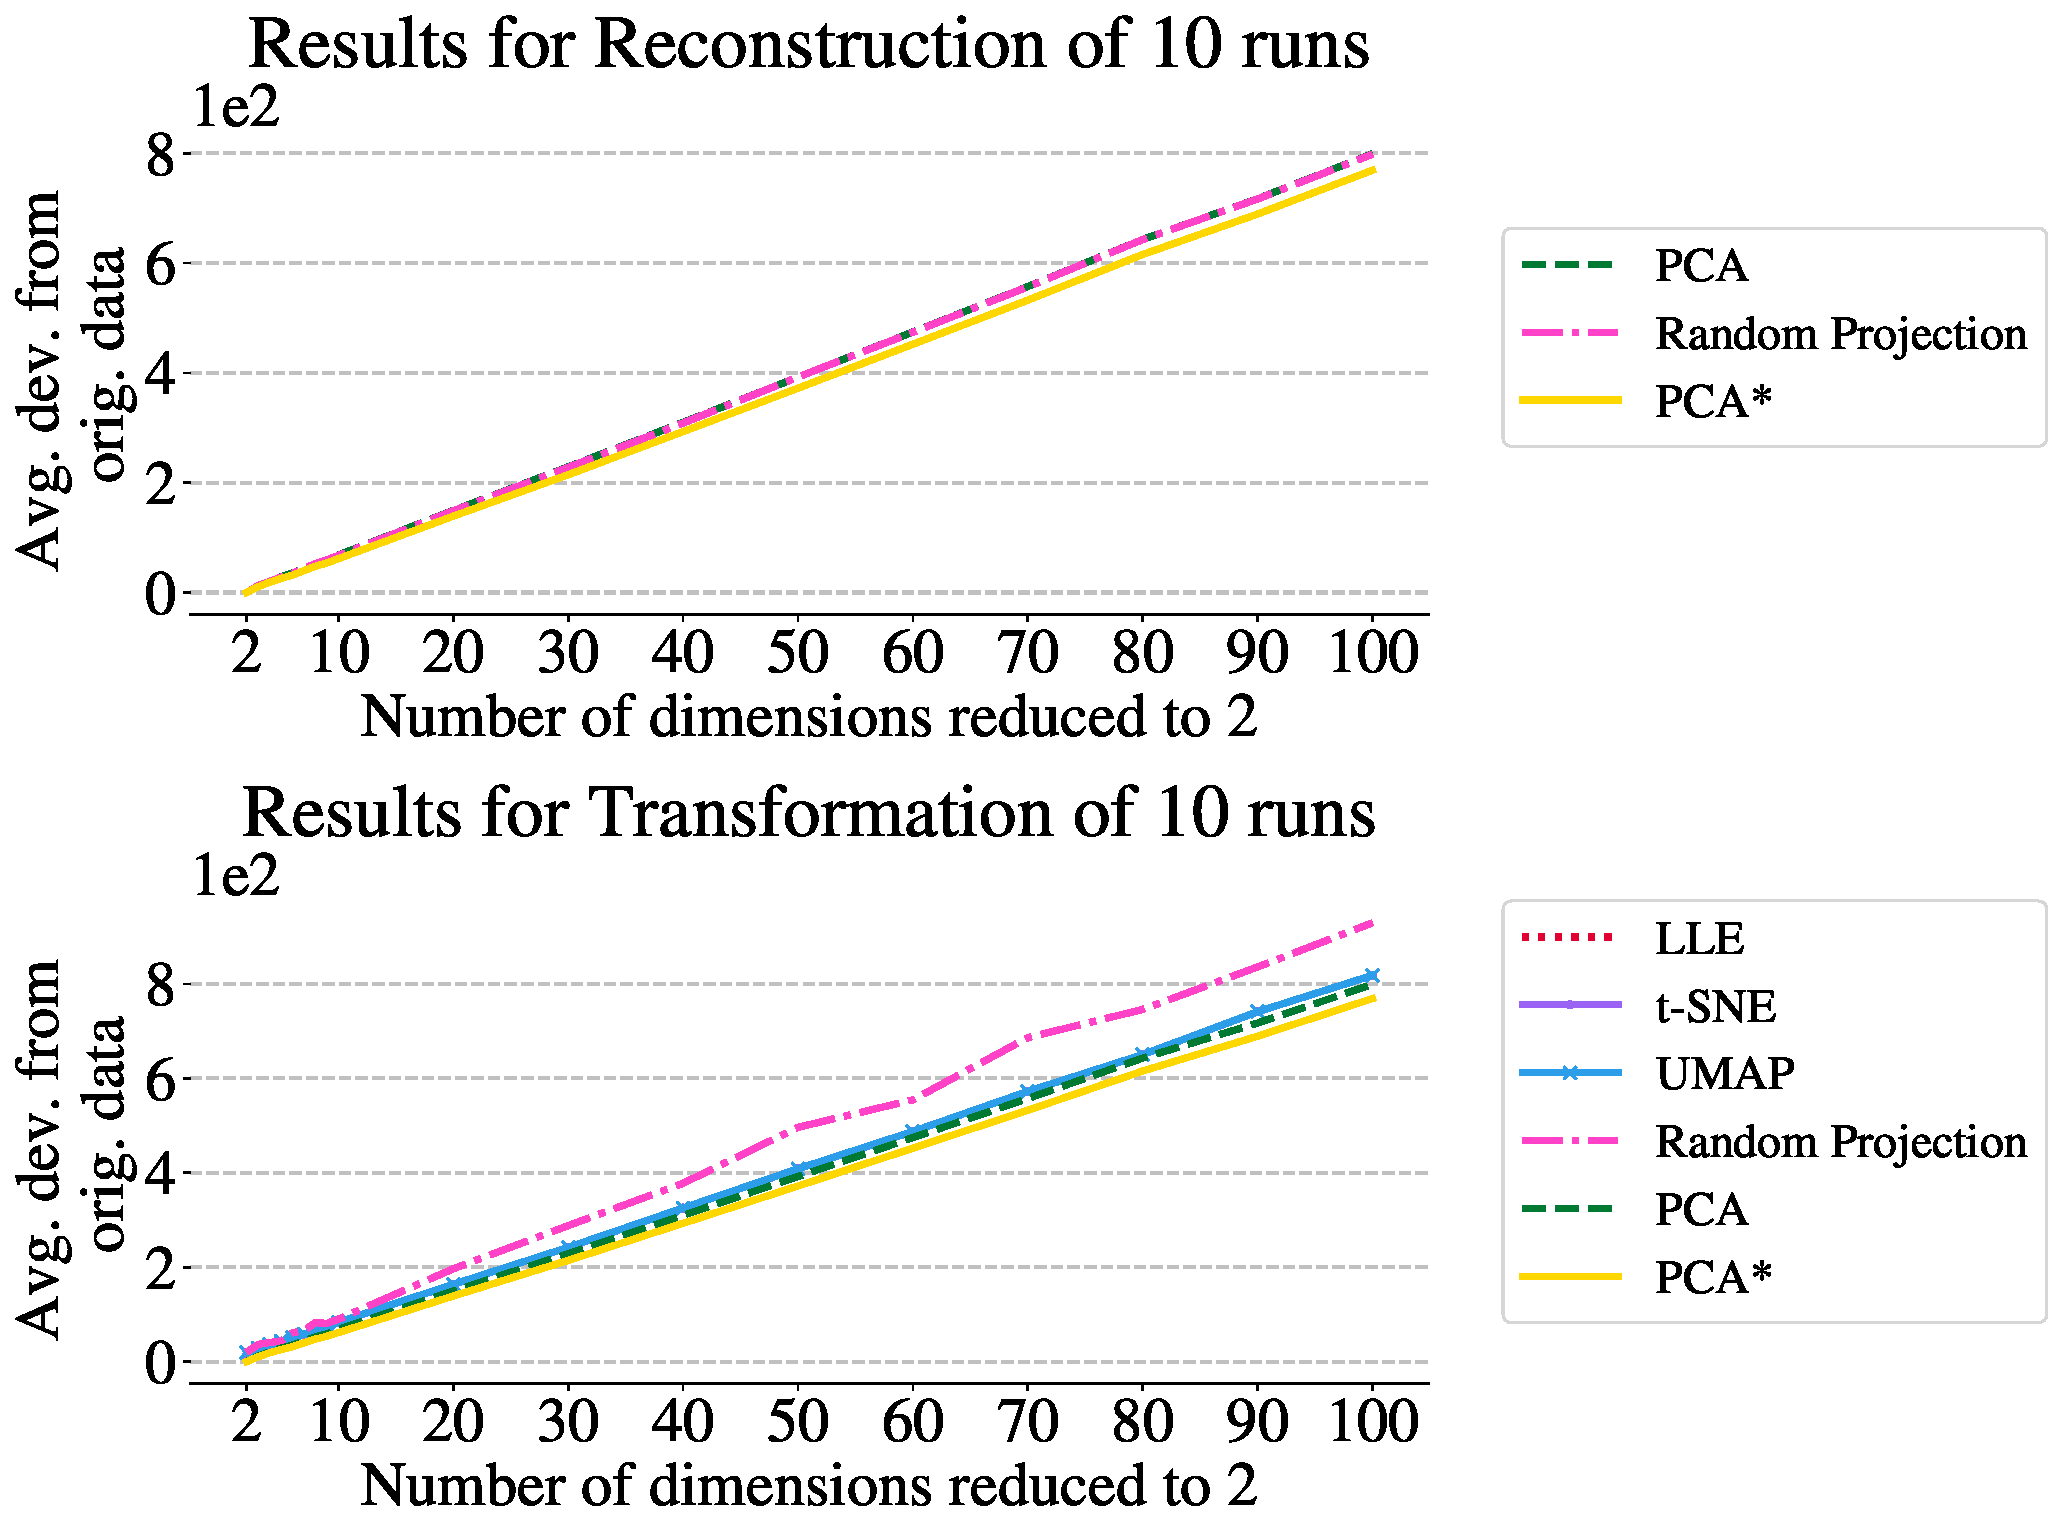
\includegraphics[width=7cm]{./images/multiple_runs/sep_lines/avg_dev_vs_dyn_high/5lines_100points_1neighbours_multiple_scalar_product.pdf}}
    \caption{Results for data in 5 separate lines: increasing the number of dimensions of the original data}\label{fig:avg_dev_vs_high_dim-seplines}
\end{figure}

Figure \ref{fig:avg_dev_vs_high_dim-seplines} presents similar results for data arranged in separate lines.
When compared to PCA, LLE, t-SNE and UMAP, PCA* shows marginally lower mean results for each measure.
As mentioned earlier, random projection prioritises local structure preservation, making it better at maintaining distances compared to PCA*, given that the order of the data is similar to their spatial distances.
However, as seen in previous results, random projection falls short in preserving relations in the transformed space compared to other observed methods. 
Additionally, its random nature is reflected in the transformed space, with higher variance than any other dimensionality reduction method.

\begin{figure}[!htb]
    \subfigure[Zigzag data]{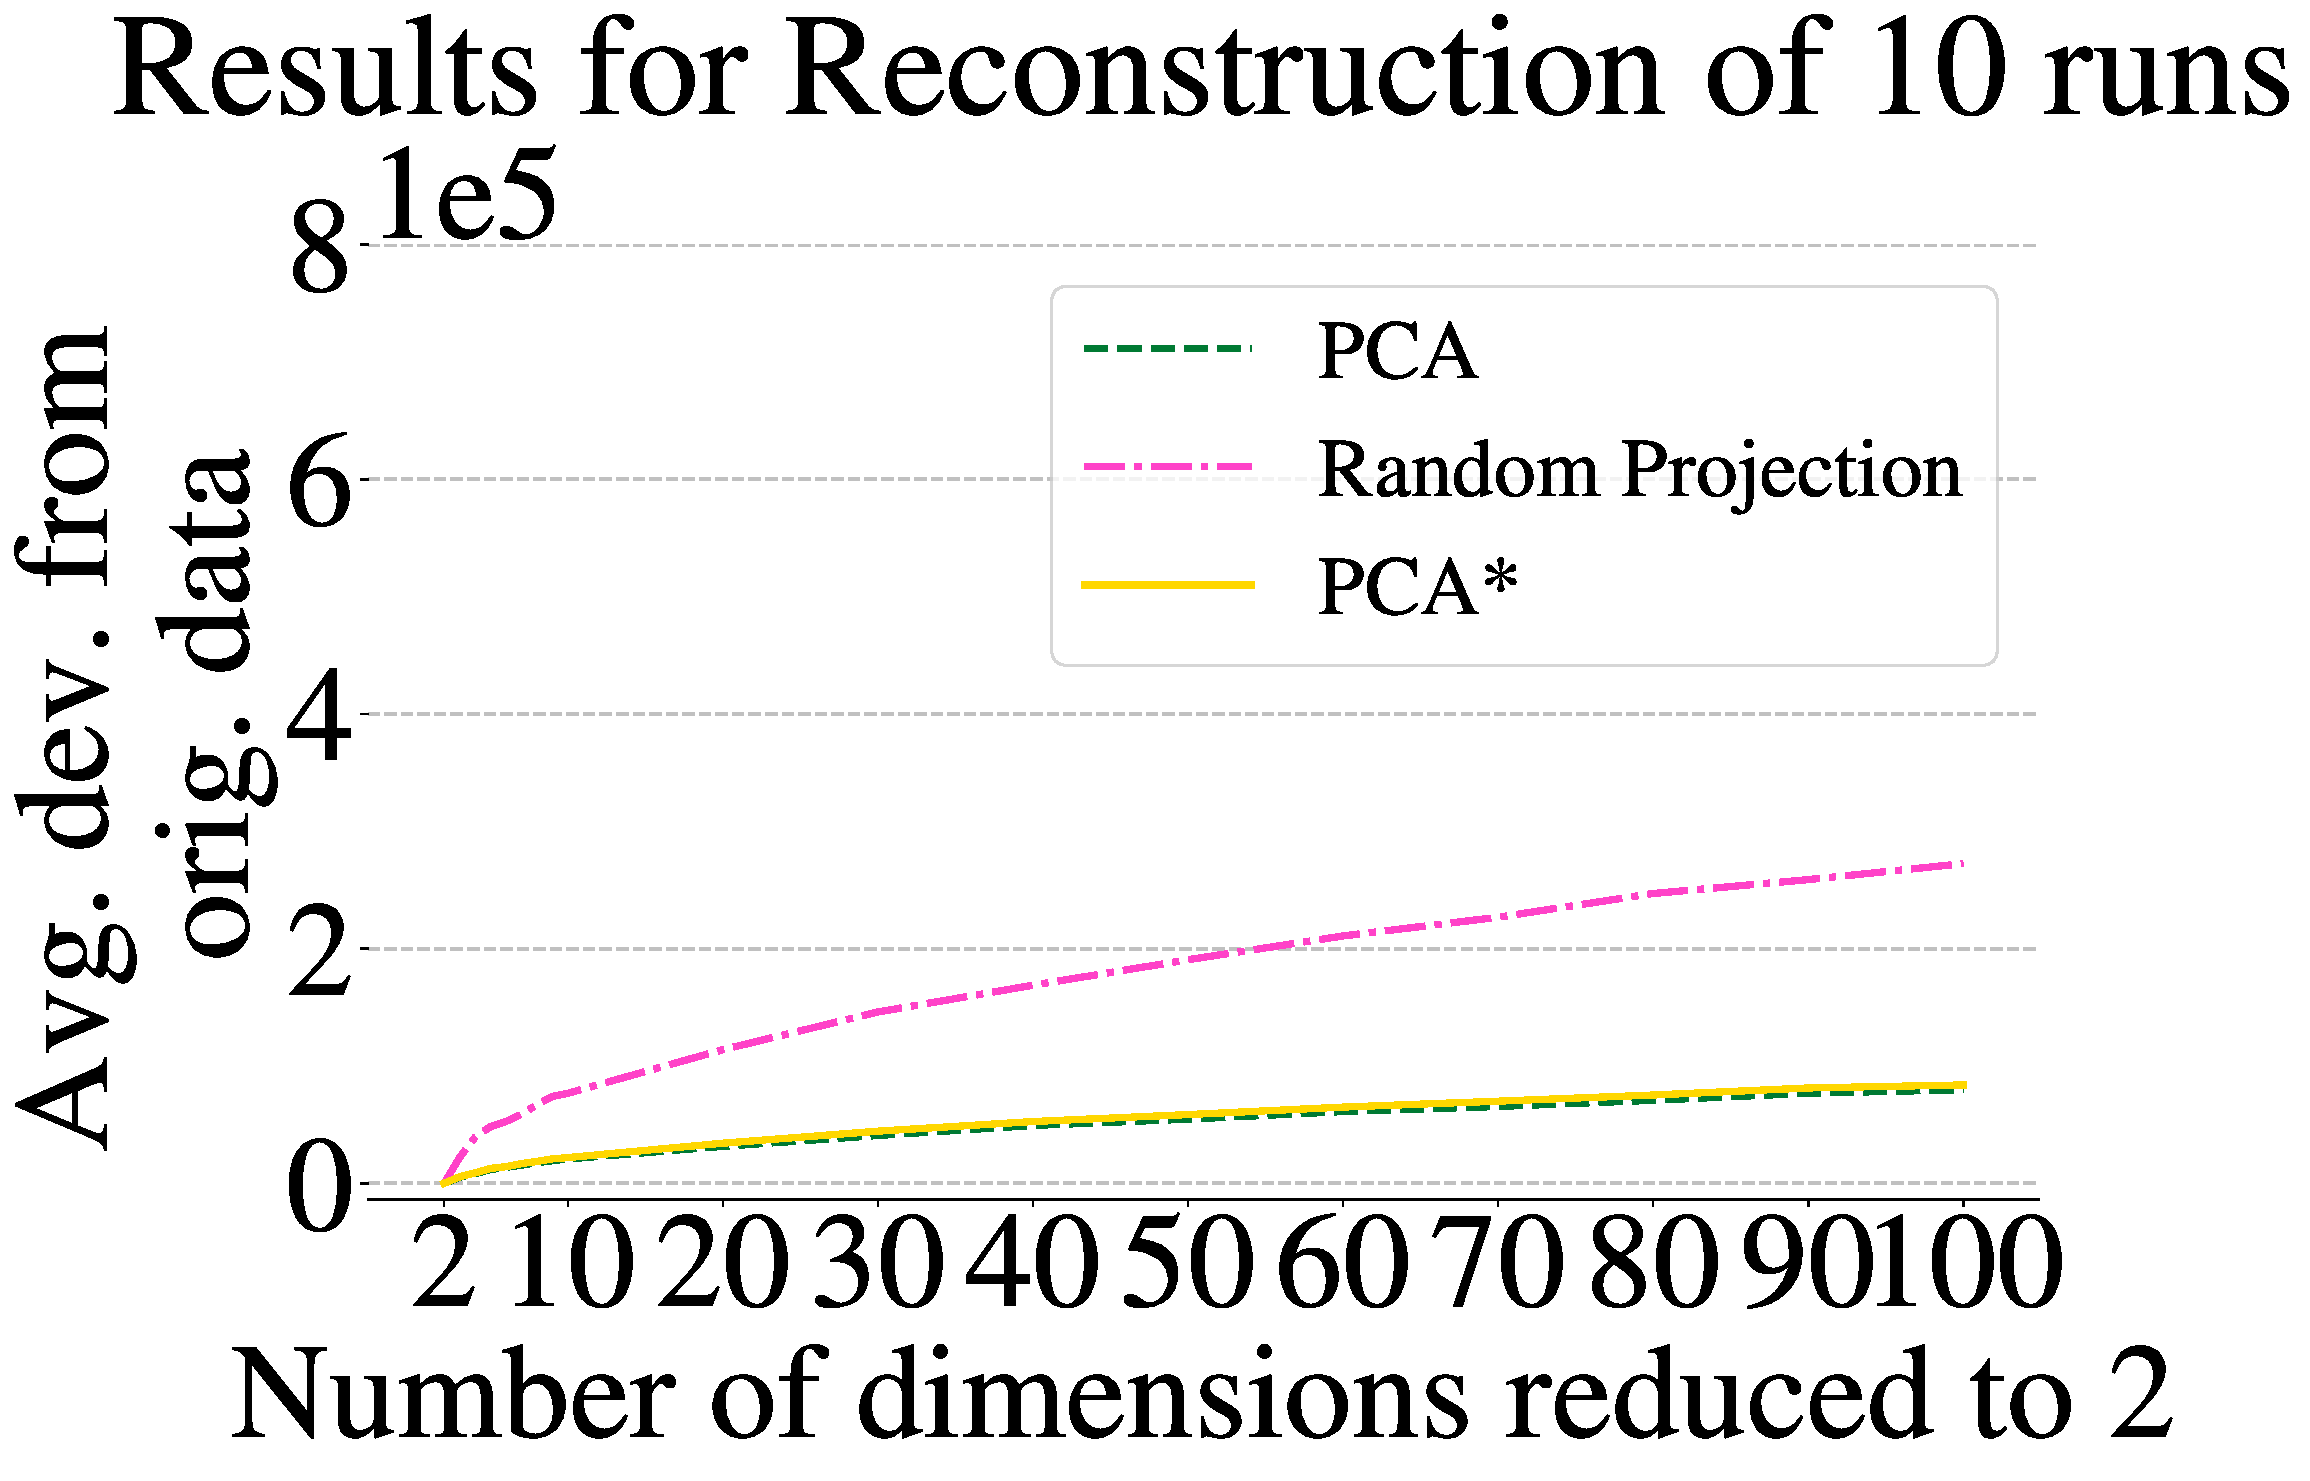
\includegraphics[width=4.45cm]{./images/multiple_runs/zigzag/avg_dev_vs_dyn_high/5lines_100points_1neighbours_dtw.pdf}}
    \subfigure[One-line data]{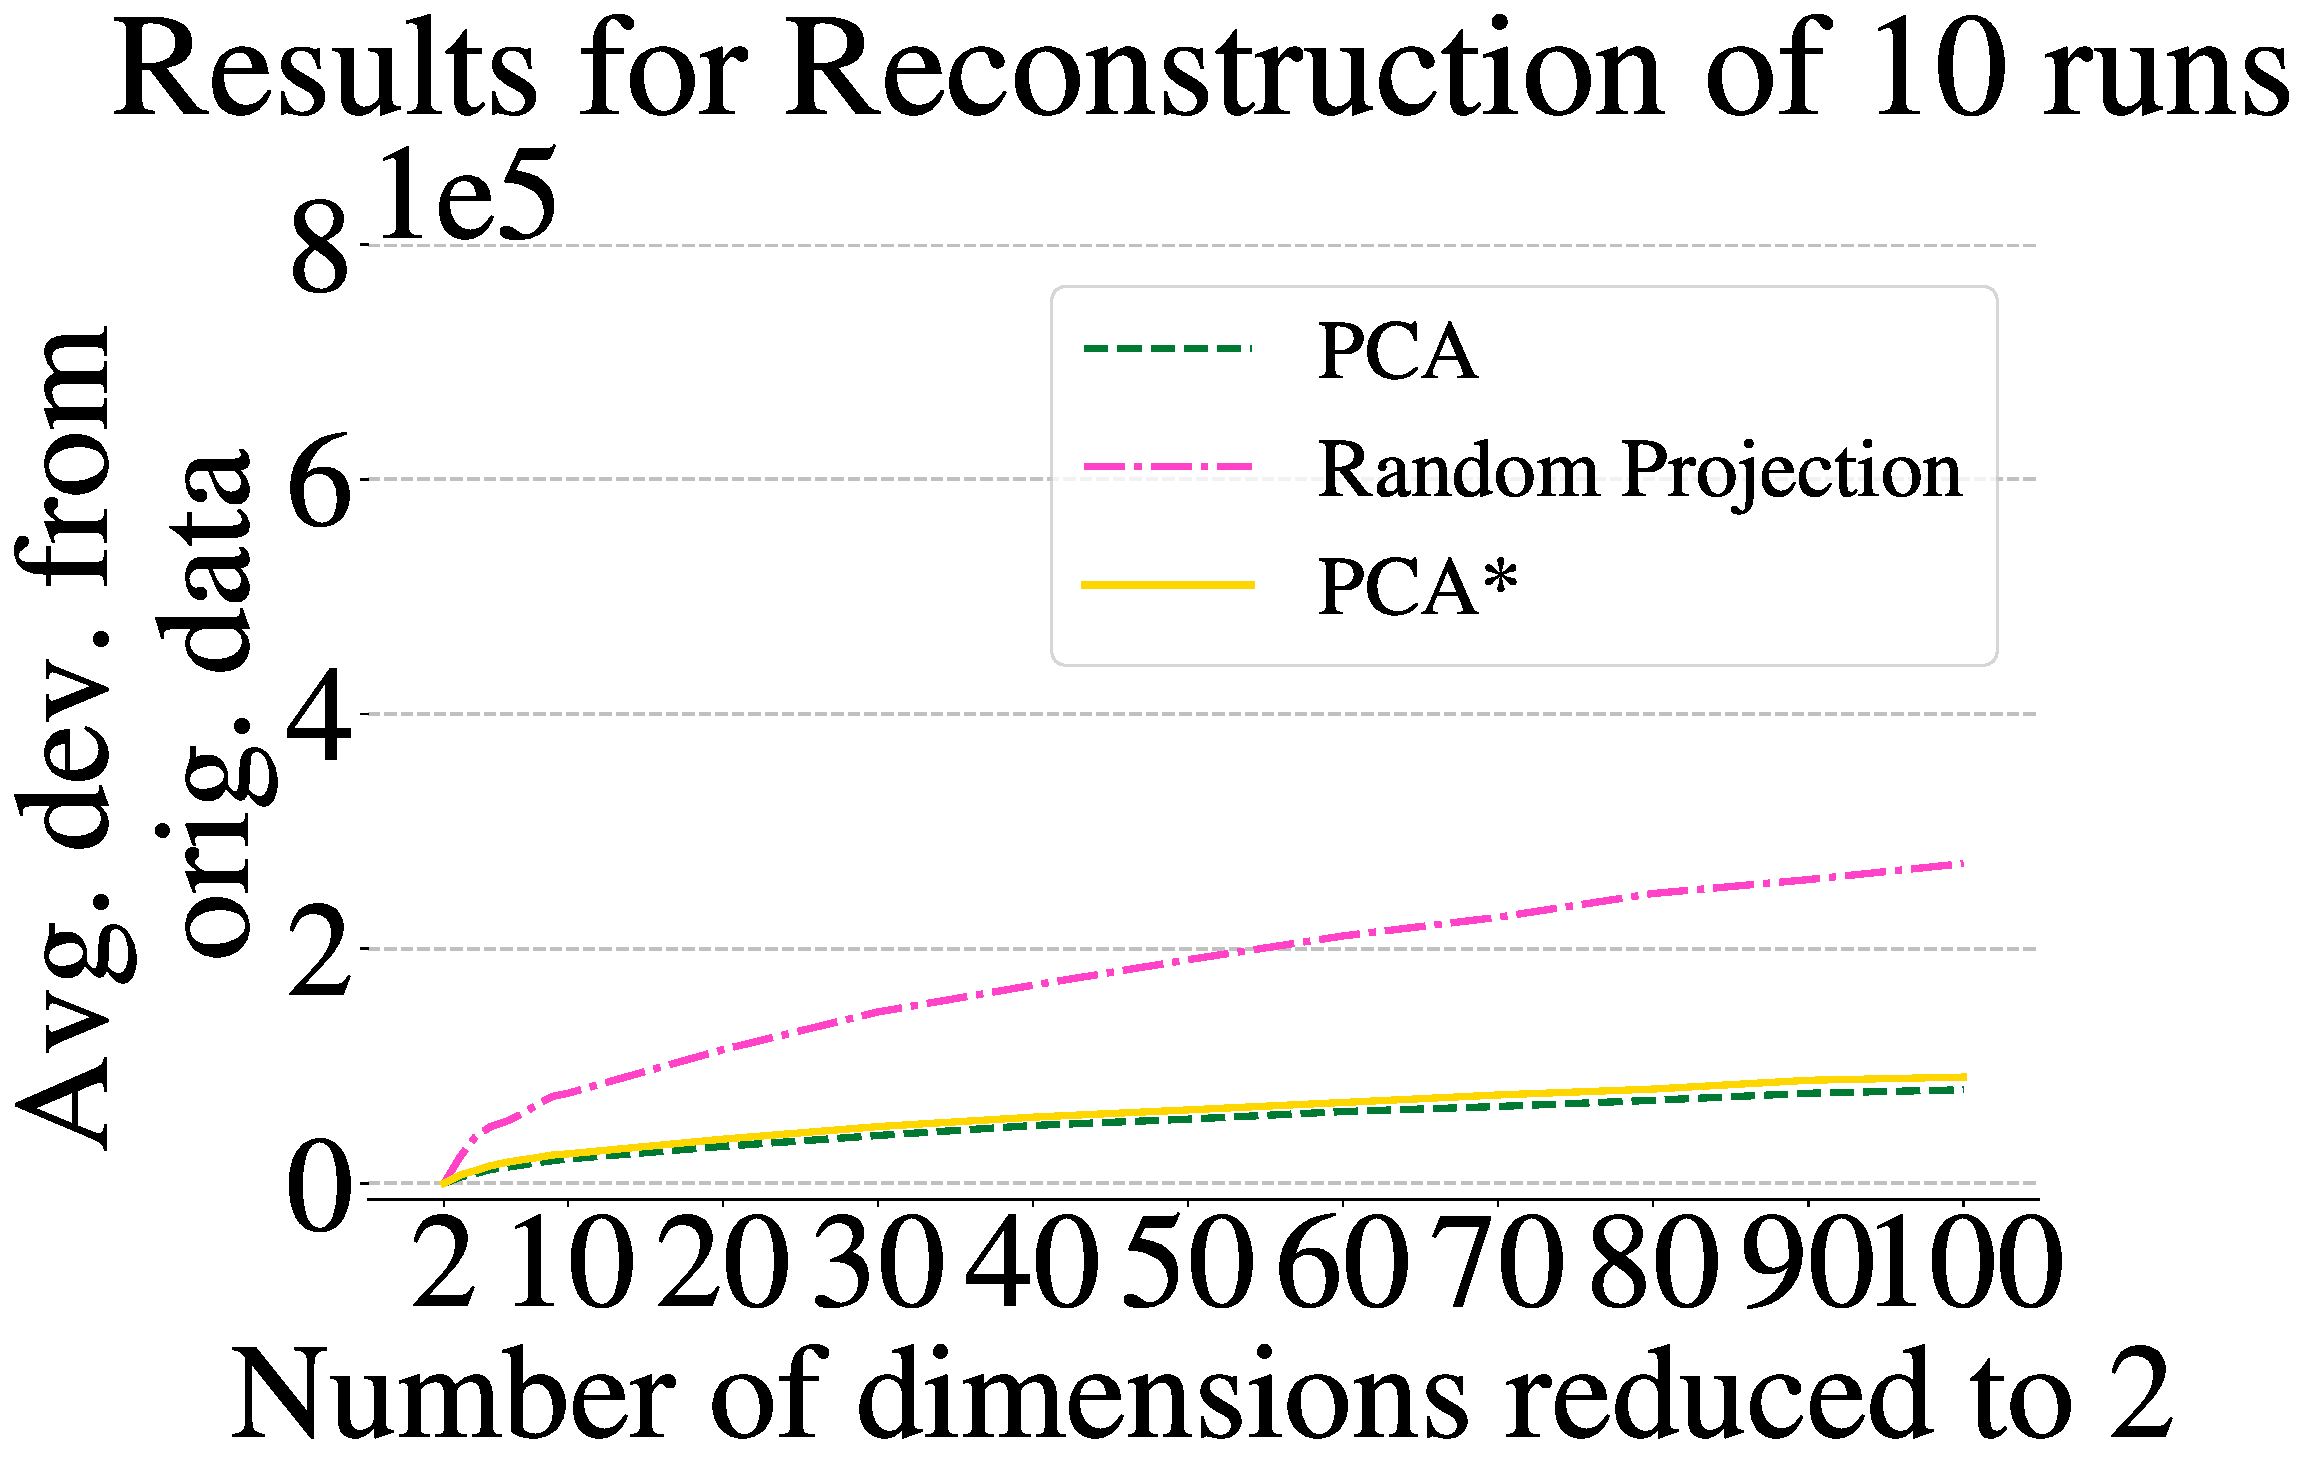
\includegraphics[width=4.45cm]{./images/multiple_runs/one_line/avg_dev_vs_dyn_high/5lines_100points_1neighbours_dtw.pdf}}
    \subfigure[Data in separate lines]{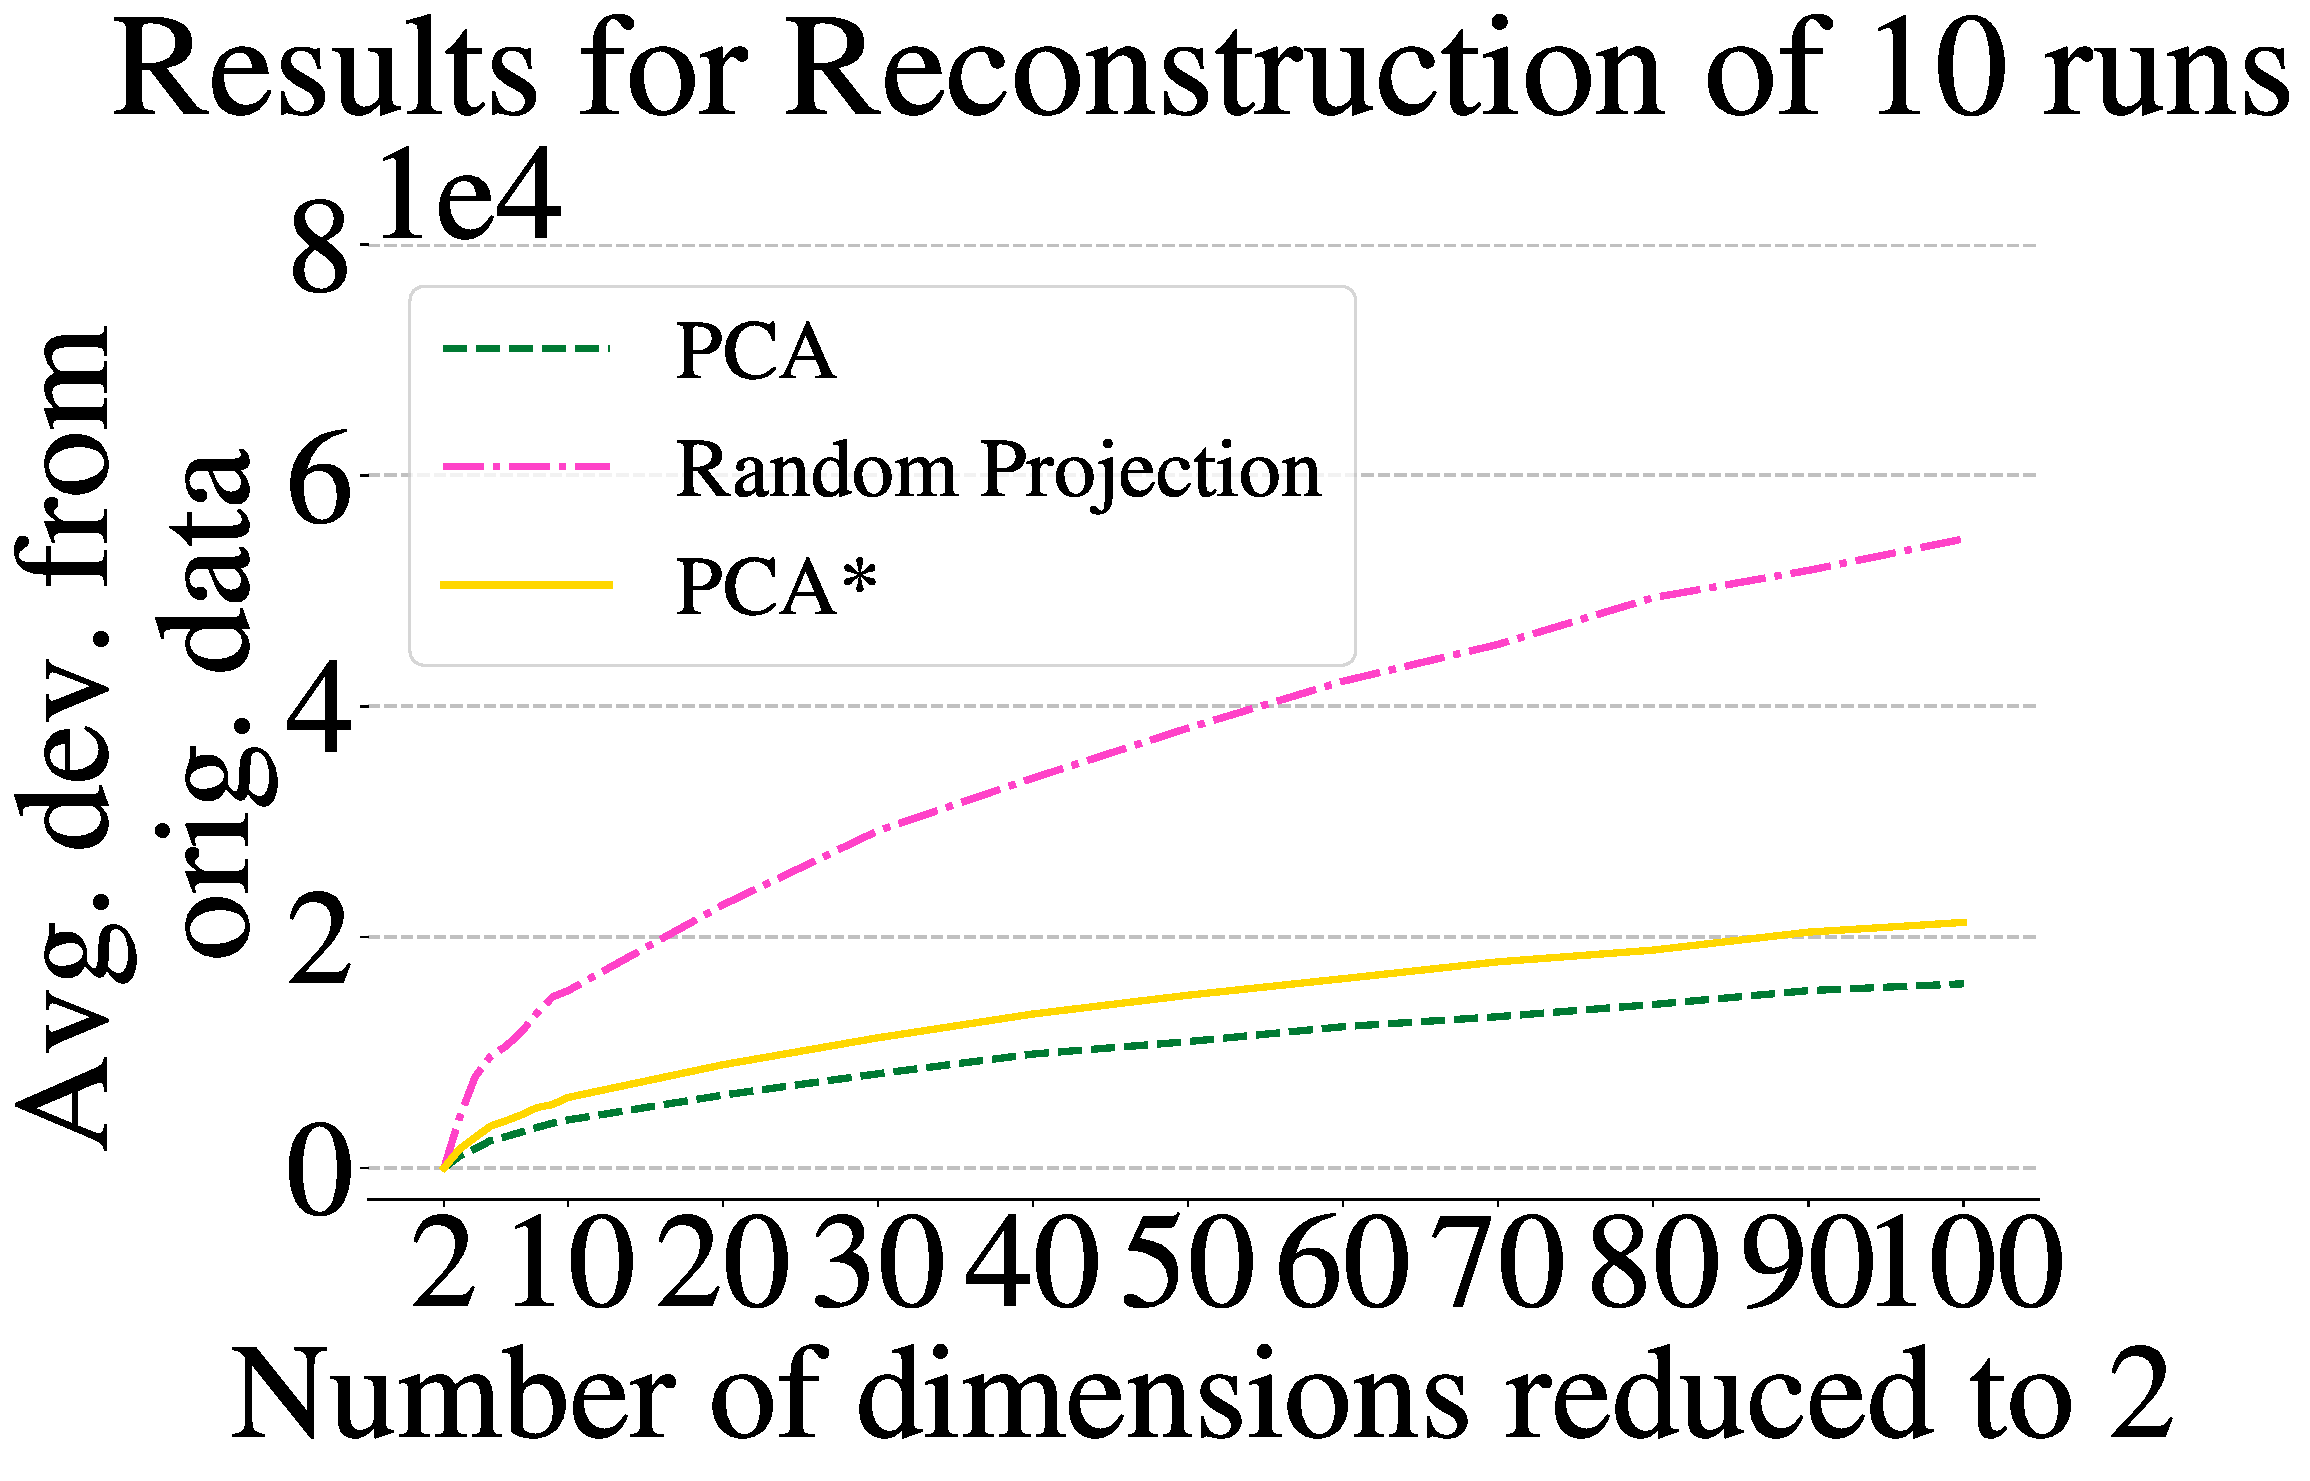
\includegraphics[width=4.45cm]{./images/multiple_runs/sep_lines/avg_dev_vs_dyn_high/5lines_100points_1neighbours_dtw.pdf}}
    \caption{Results for data in different orders measured with DTW: increasing the number of dimensions of the original data}\label{fig:avg_dev_vs_high_dim-dtw}
\end{figure}
\FloatBarrier

Finally, we compare the results of the dimensionality reduction methods with DTW, see Figure~\ref{fig:avg_dev_vs_high_dim-dtw}.
For each order, PCA* shows similar results as PCA whereas random projection exhibits substantially worse results.
This may be because random projection transforms data onto lower-dimensional space by applying random linear transformation without taking into account the intrinsic structure of the data.

\subsection{Expanding the Dimensionality of the Transformation} \label{sec:avg_dev_vs_dyn_low_dims}

In this experiment, we apply dimensionality reduction methods to the 100-dimensional dataset while systematically increasing the number of dimensions in the transformed space.
We start with a reduced dimensionality of two and gradually increase it up to the original number of dimensions.
To assess the quality of the dimensionality reduction techniques, we conduct a comparison between the transformed and original data, and analogously the reconstructed and original data.
This evaluation involves computing the average deviation for each summed distance between each point and its predecessor and successor, employing the quality measures in Section~\ref{quality-measures}.
With this experiment, we determine the optimal number of dimensions to which the dataset should be transformed.
By varying the dimensionality, we gain insights into how dimensionality reduction impacts the dataset's overall quality and structure.

\begin{figure}[!htb]
    \subfigure[Neighbour-Distance Measure]{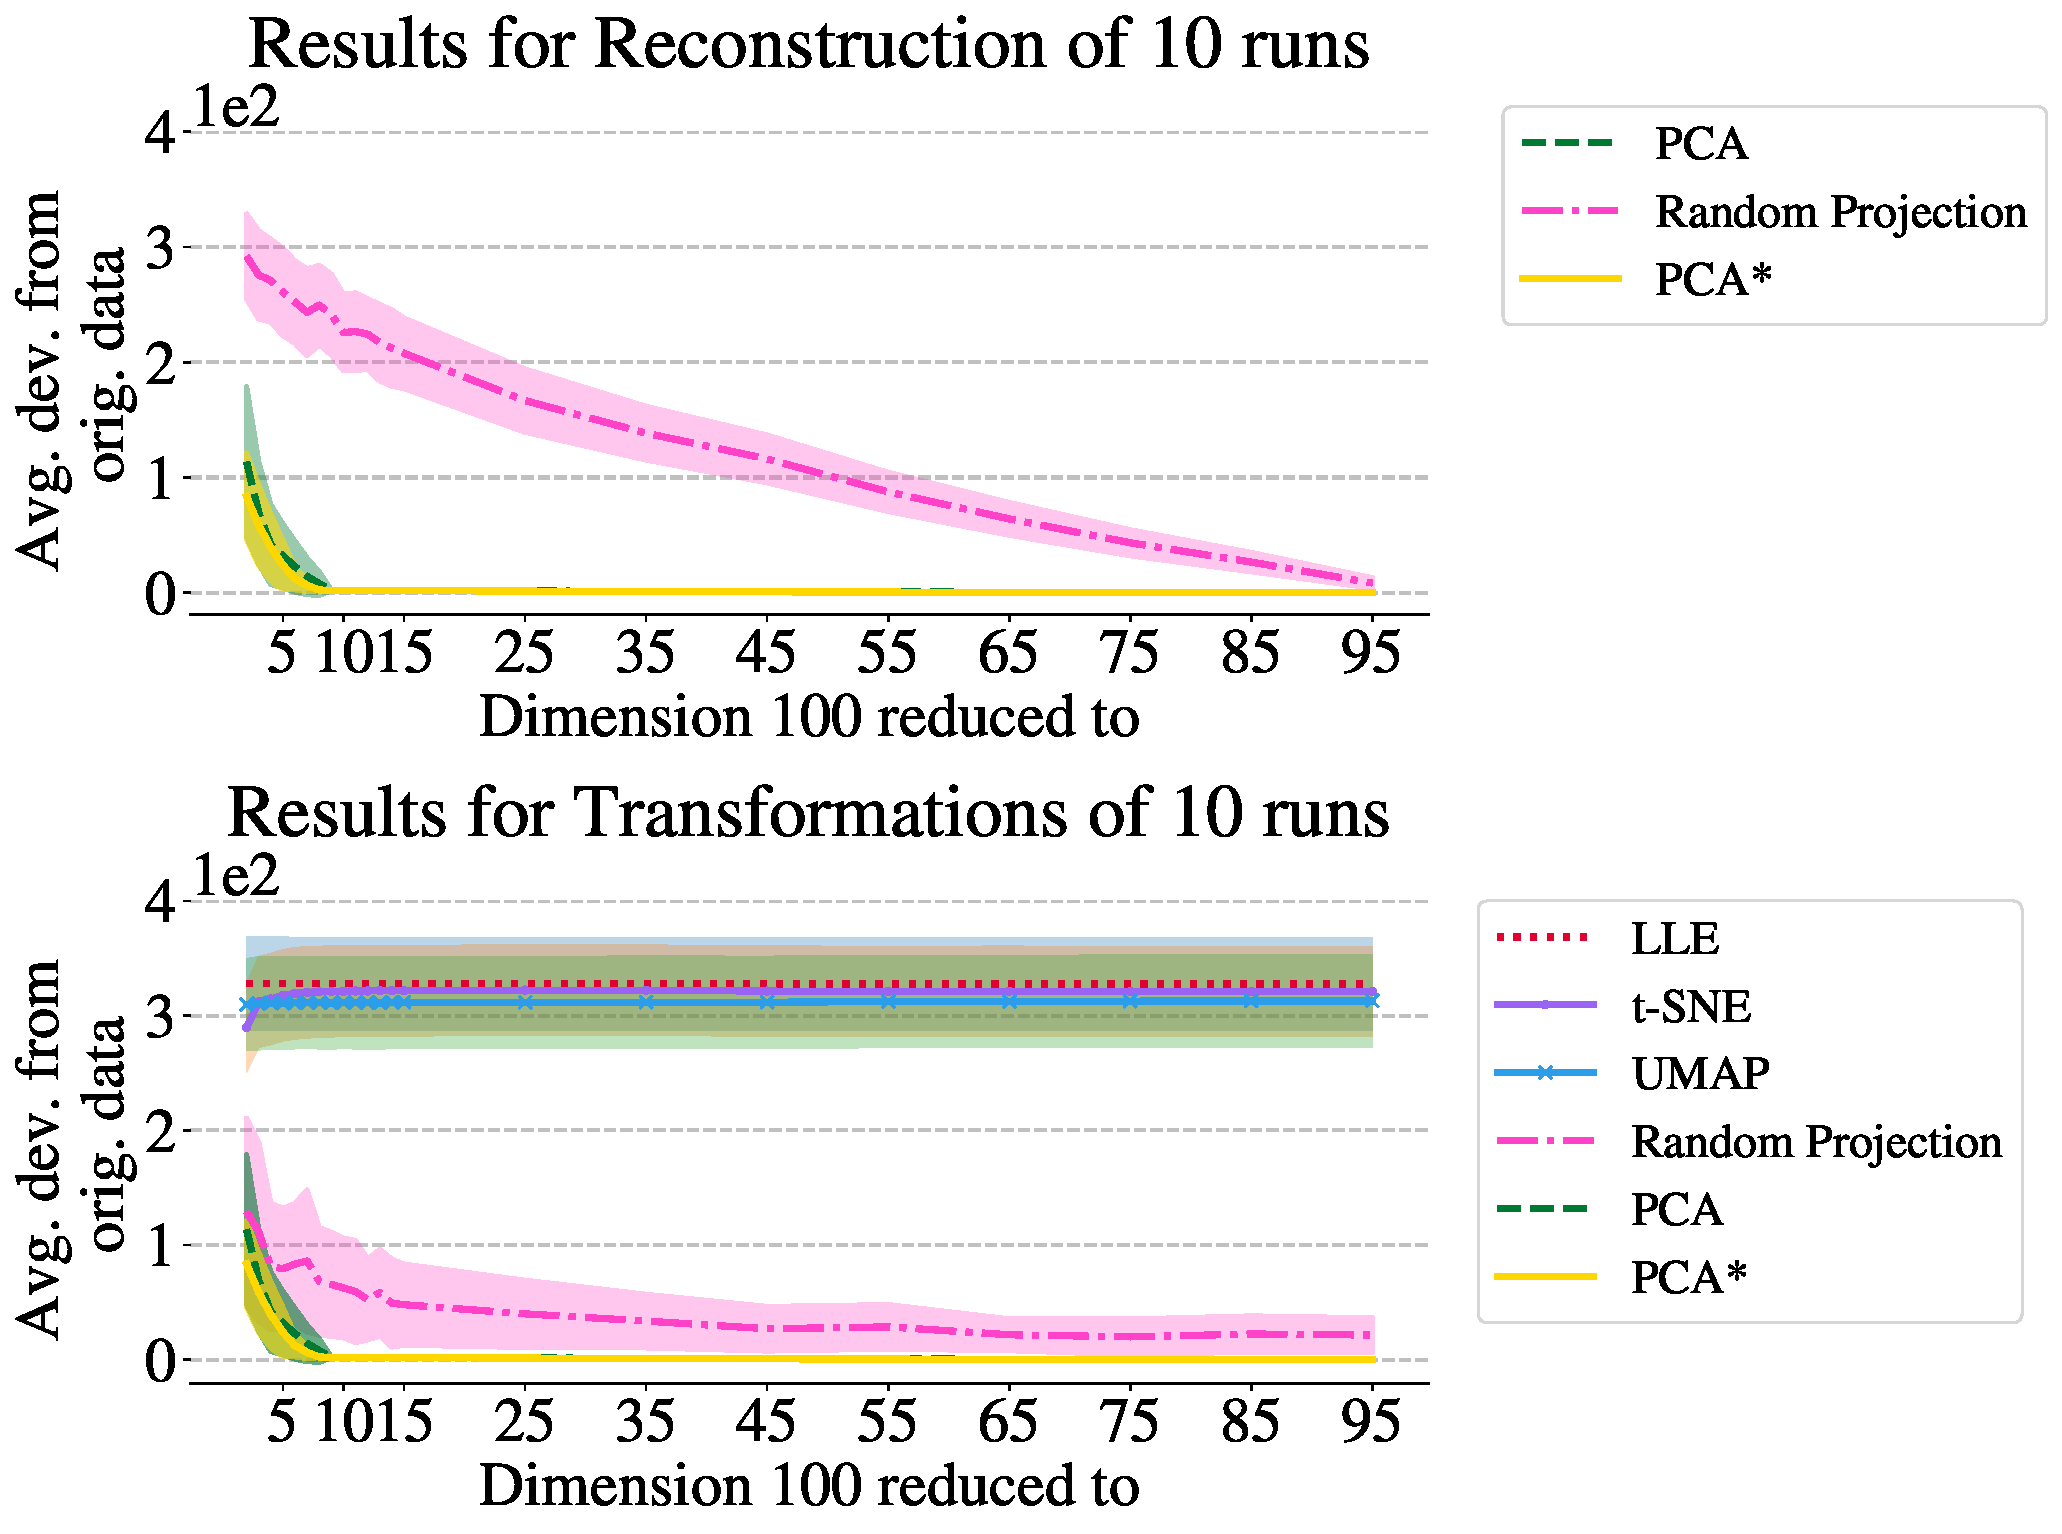
\includegraphics[width=8cm]{./images/multiple_runs/zigzag/avg_dev_vs_dyn_low/5lines_100points_1neighbours_euclidean.pdf}}
    \subfigure[Neighbour-Relation measure]{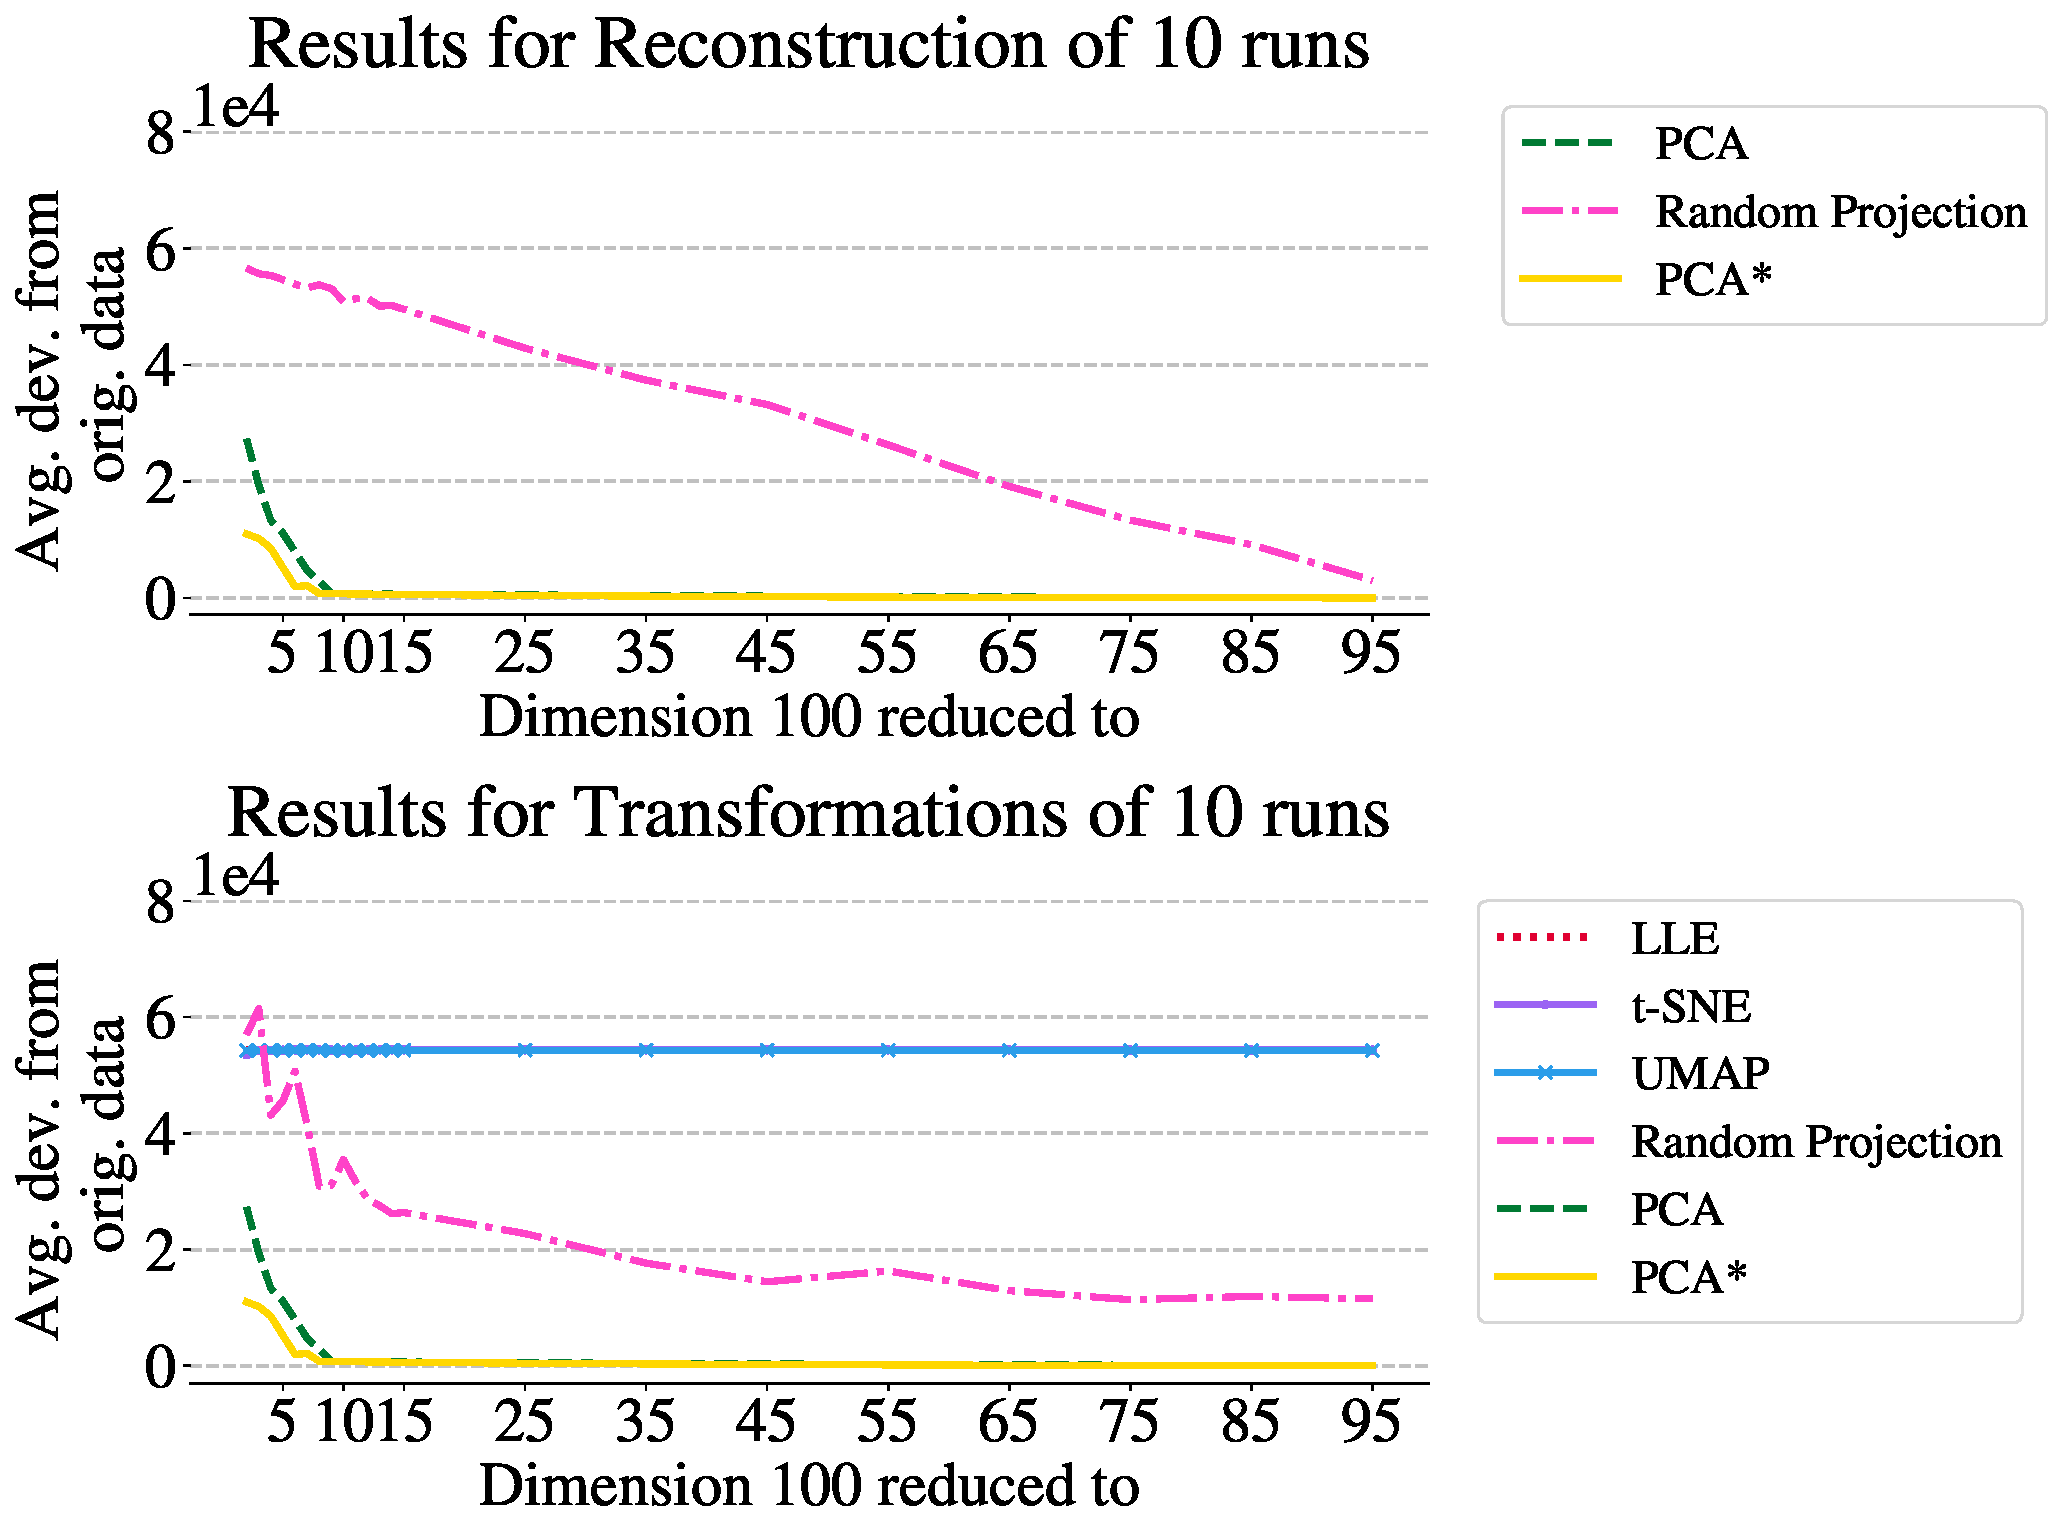
\includegraphics[width=8cm]{./images/multiple_runs/zigzag/avg_dev_vs_dyn_low/5lines_100points_1neighbours_scalar_product.pdf}}
    \caption{Results for zigzag data: increasing the number of dimensions of the lower-dimensional space}\label{fig:avg_dev_dyn_low_zigzag}
\end{figure}

When we compare all dimensionality reduction techniques applied to zigzag data, we observe that random projection performs less effectively than both PCA and PCA*, as shown in Figure~\ref{fig:avg_dev_dyn_low_zigzag}.
Interestingly, the results of LLE, t-SNE and UMAP do exhibit significant variations.
This could be attributed to the fact that we did not fine-tune the parameters of these techniques and instead relied on default values.
For instance, sklearn's implementation of t-SNE uses a default perplexity value of 30, which is associated with the number of the spatial nearest neighbours considered in other dimensionality reduction methods \cite{website-tsne}.
Given that LLE, t-SNE and UMAP are local structure-preserving methods, they tend to maintain distances to spatially nearest neighbours.
In other words, these methods try to maintain the distance to the spatially nearest neighbours, they aim to keep the same distance for all lower dimensionalities.
Therefore the results remain constant for each number of dimensions to which the data is transformed.

\begin{figure}[!htb]
    \subfigure[Neighbour-Distance Measure]{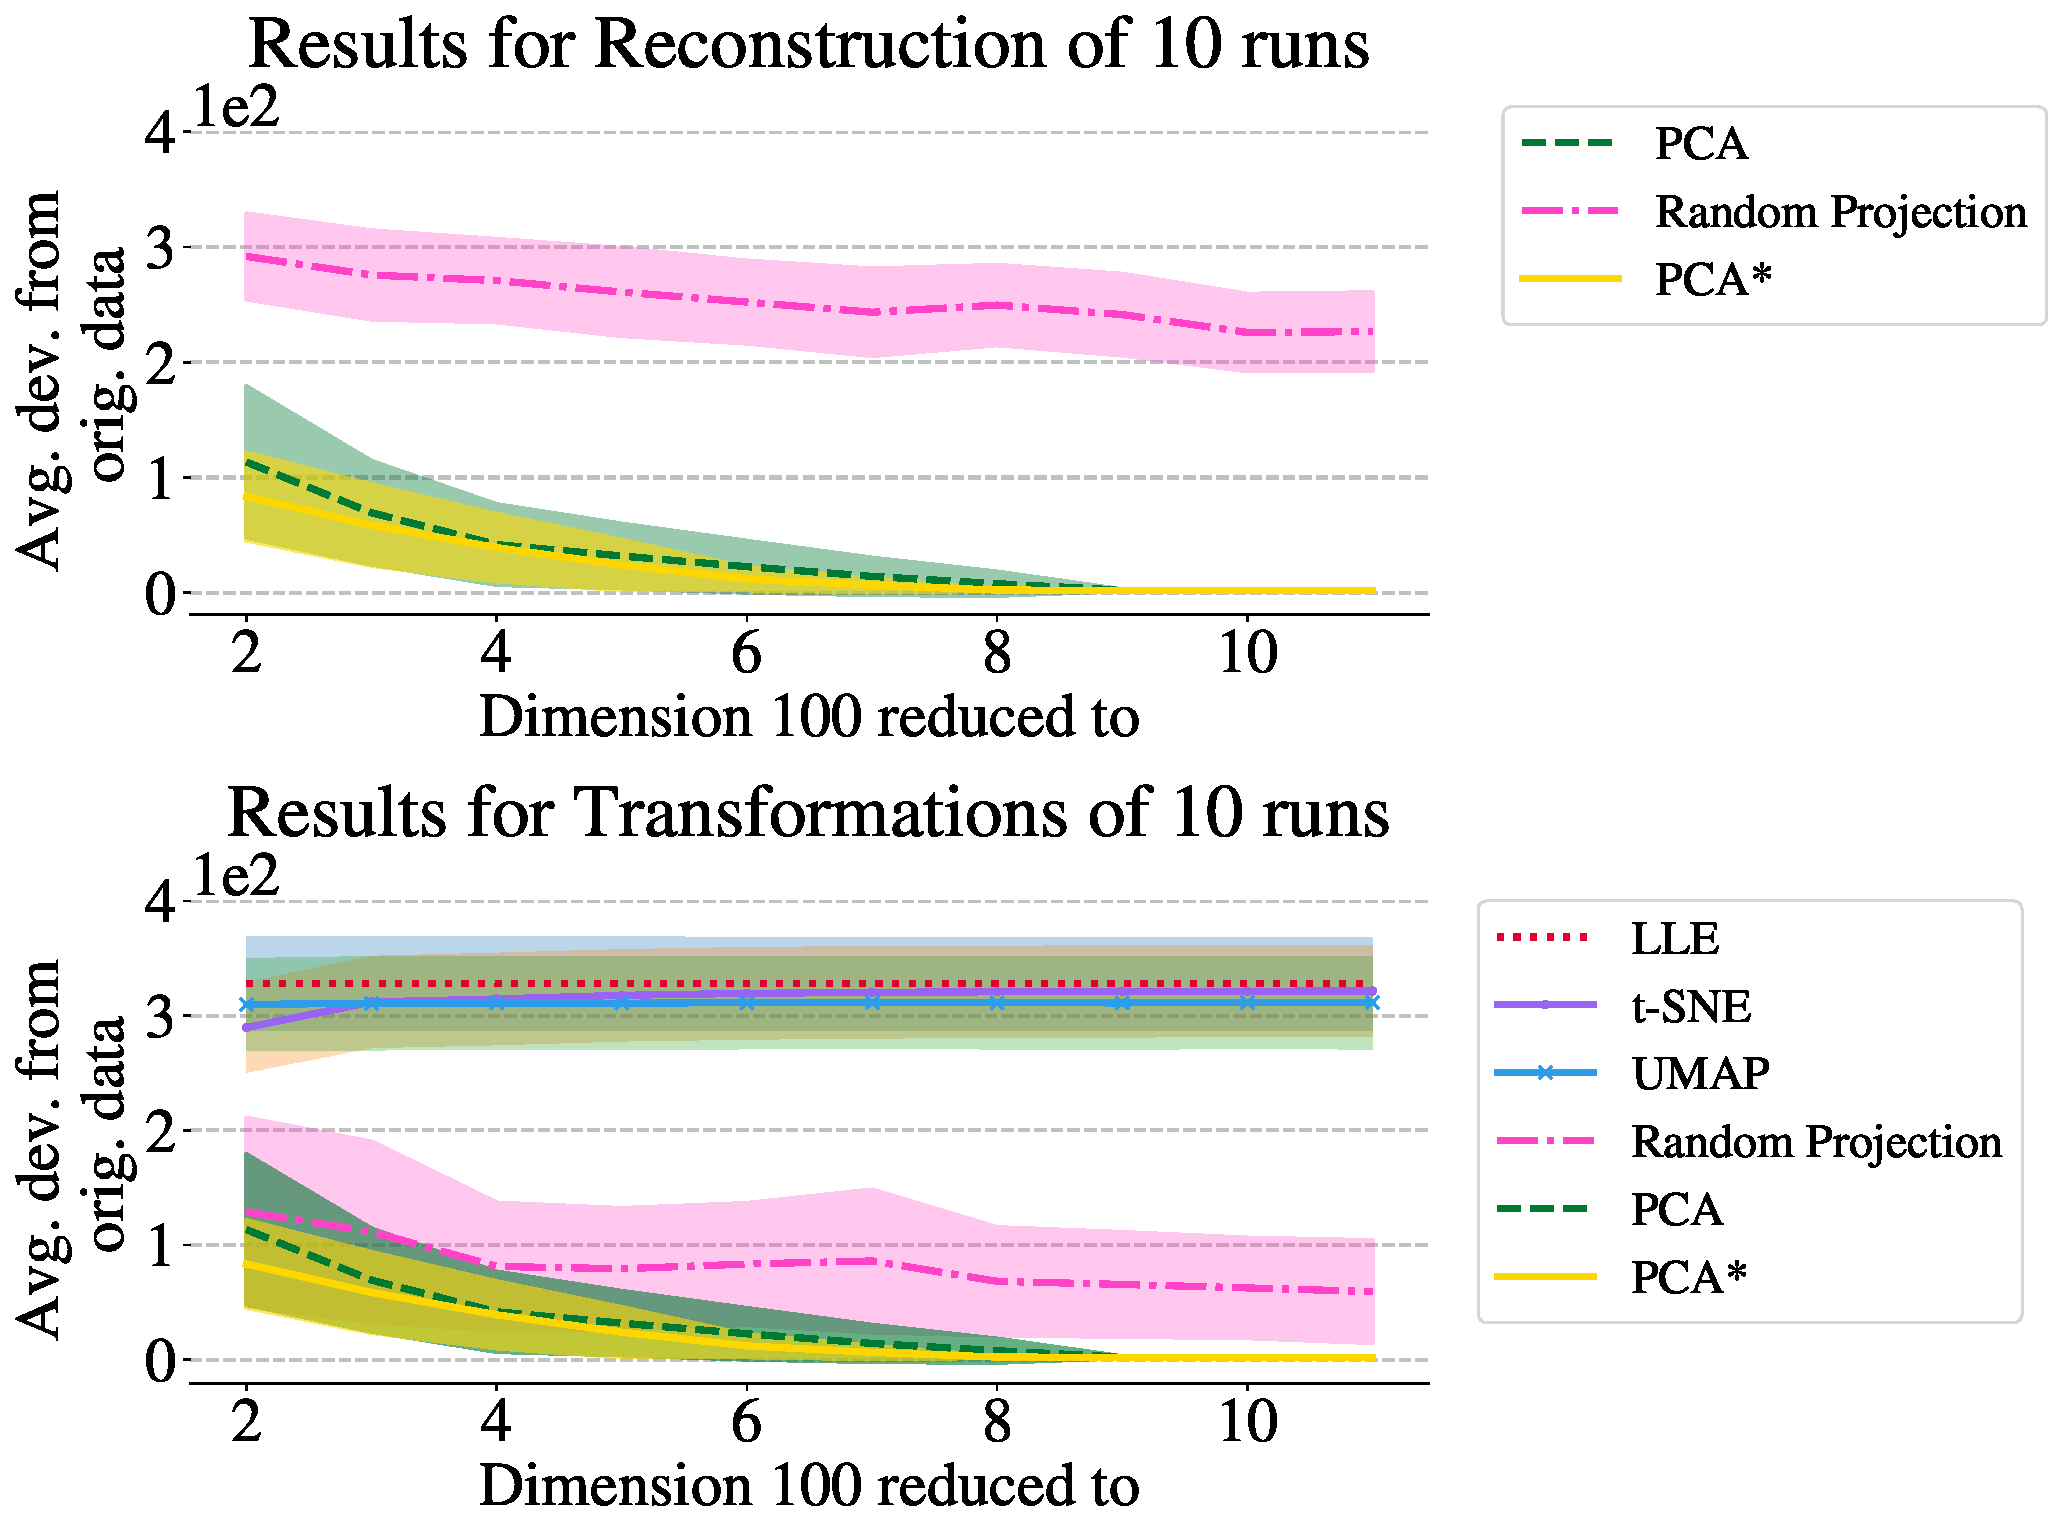
\includegraphics[width=7cm]{./images/multiple_runs/zigzag/avg_dev_vs_dyn_low/5lines_100points_1neighbours_euclidean_cutk10.pdf}}
    \subfigure[Neighbour-Relation measure]{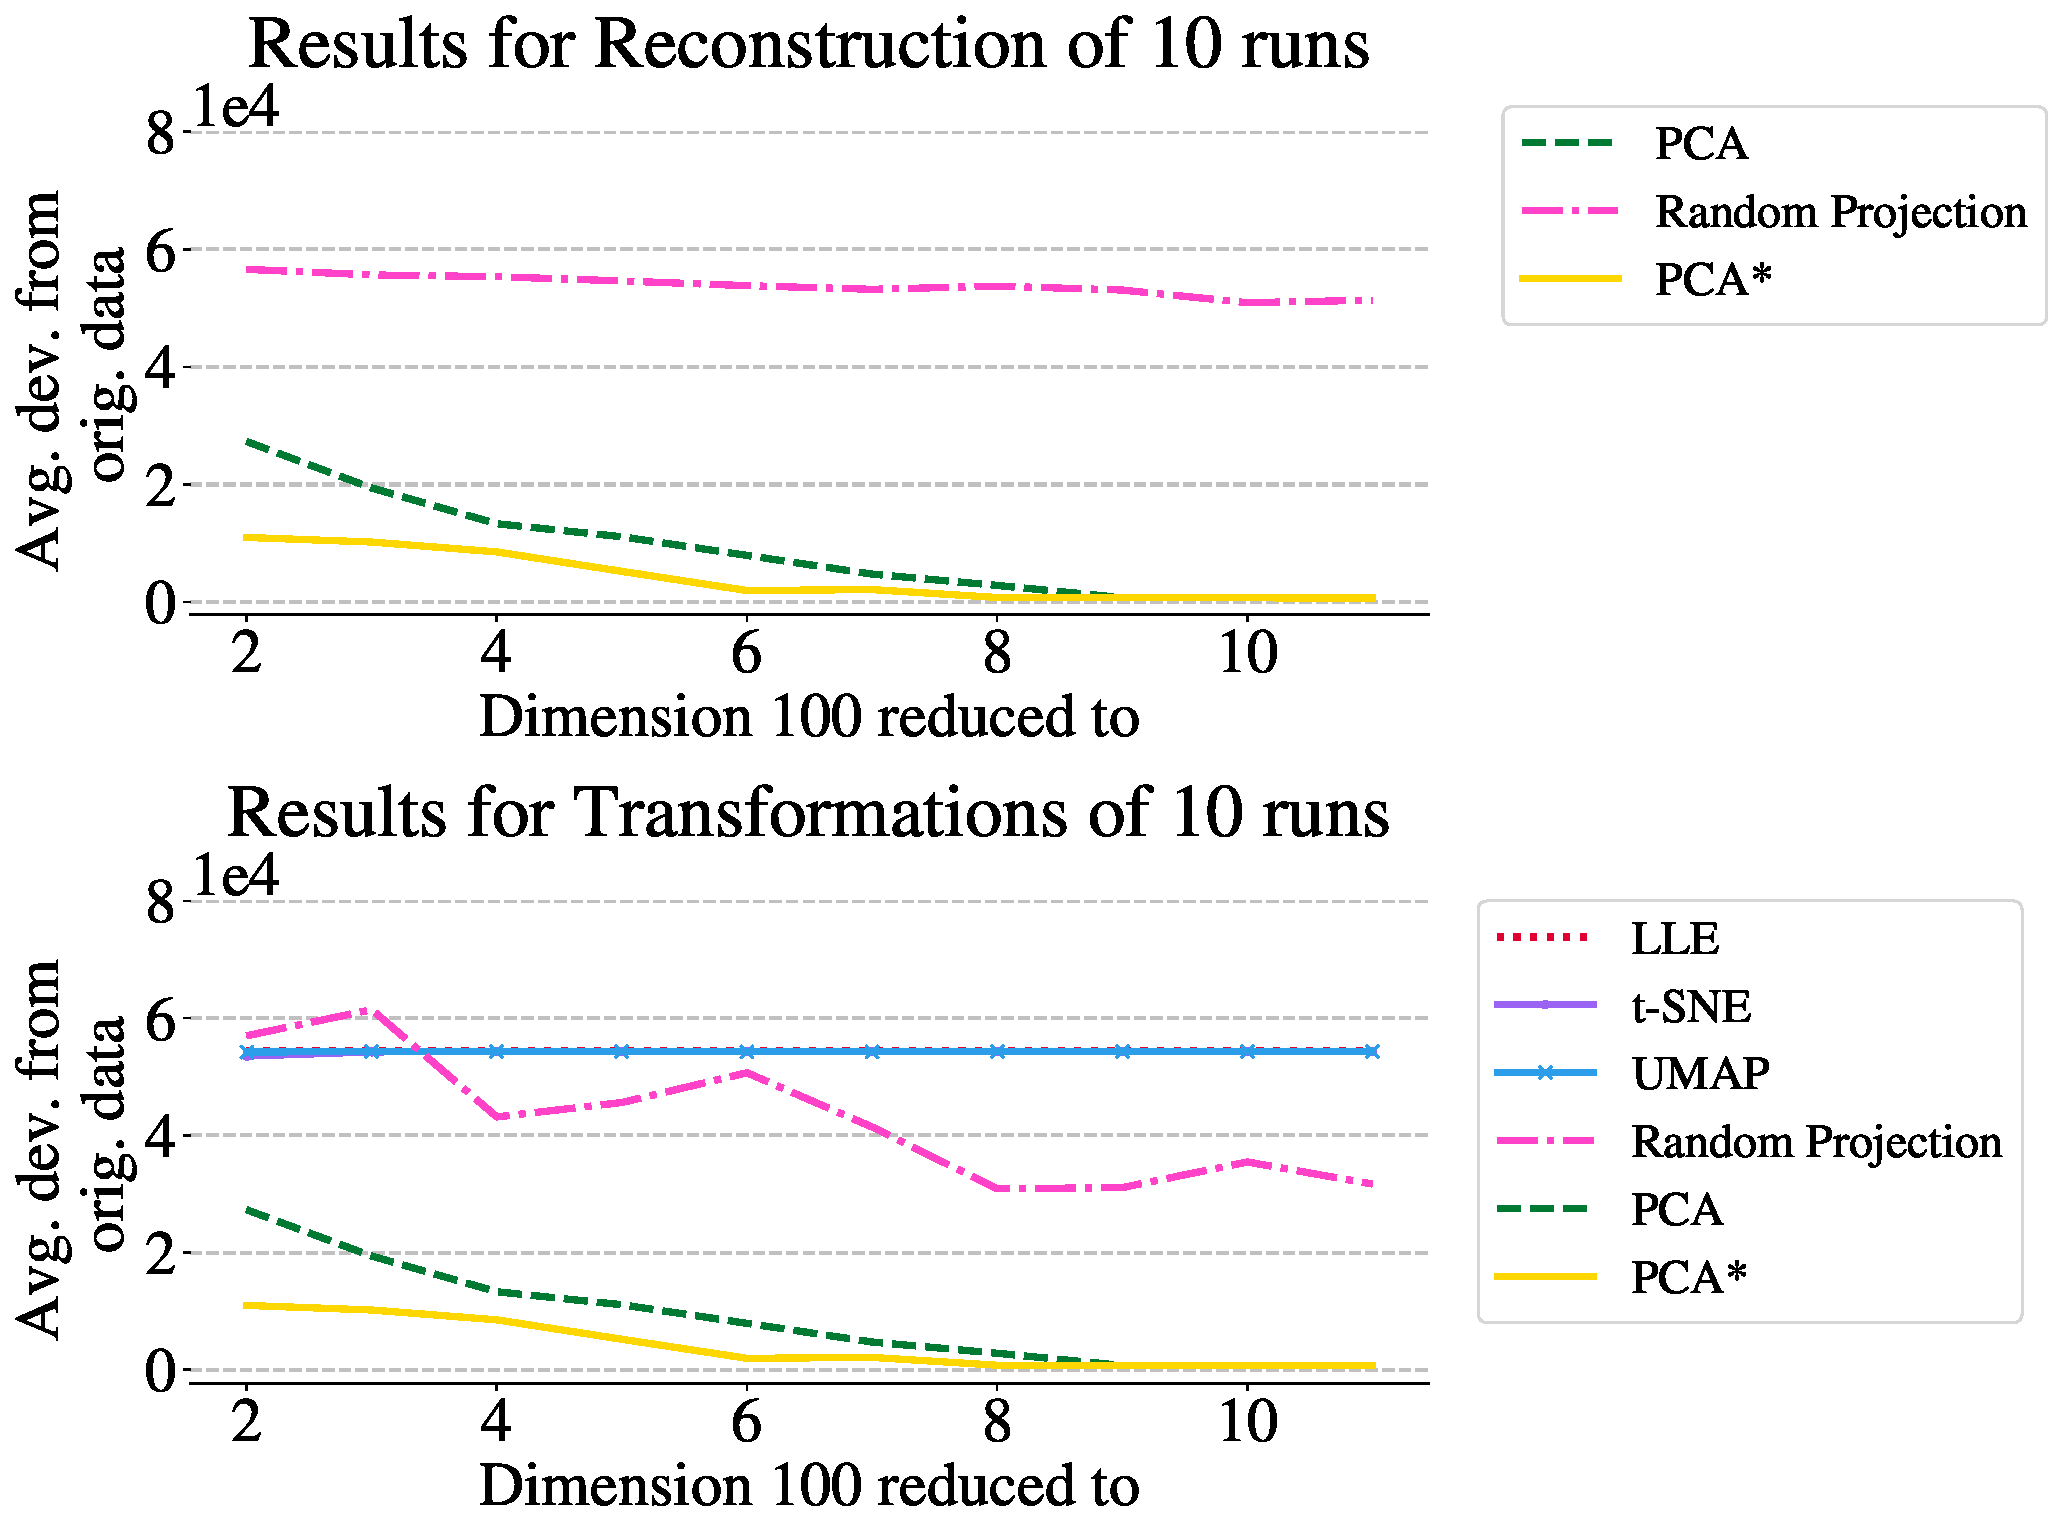
\includegraphics[width=7cm]{./images/multiple_runs/zigzag/avg_dev_vs_dyn_low/5lines_100points_1neighbours_scalar_product_cutk10.pdf}}
    \caption{Results for zigzag data: increasing the number of dimensions between 2 and 10 for the lower-dimensional space}\label{fig:avg_dev_dyn_low_zigzag_zoom}
\end{figure}
As data visualisation is only feasible in lower than 3 dimensions, we explore the range from 2 to 10 in Figure~\ref{fig:avg_dev_dyn_low_zigzag_zoom}.
PCA* outperforms PCA and random projection for lower dimensions, exhibiting lower variance in the ND measure.
This holds for both measures, especially for lower dimensions up to approximately eight.

\begin{figure}[!htb]
    \subfigure[Neighbour-Distance Measure]{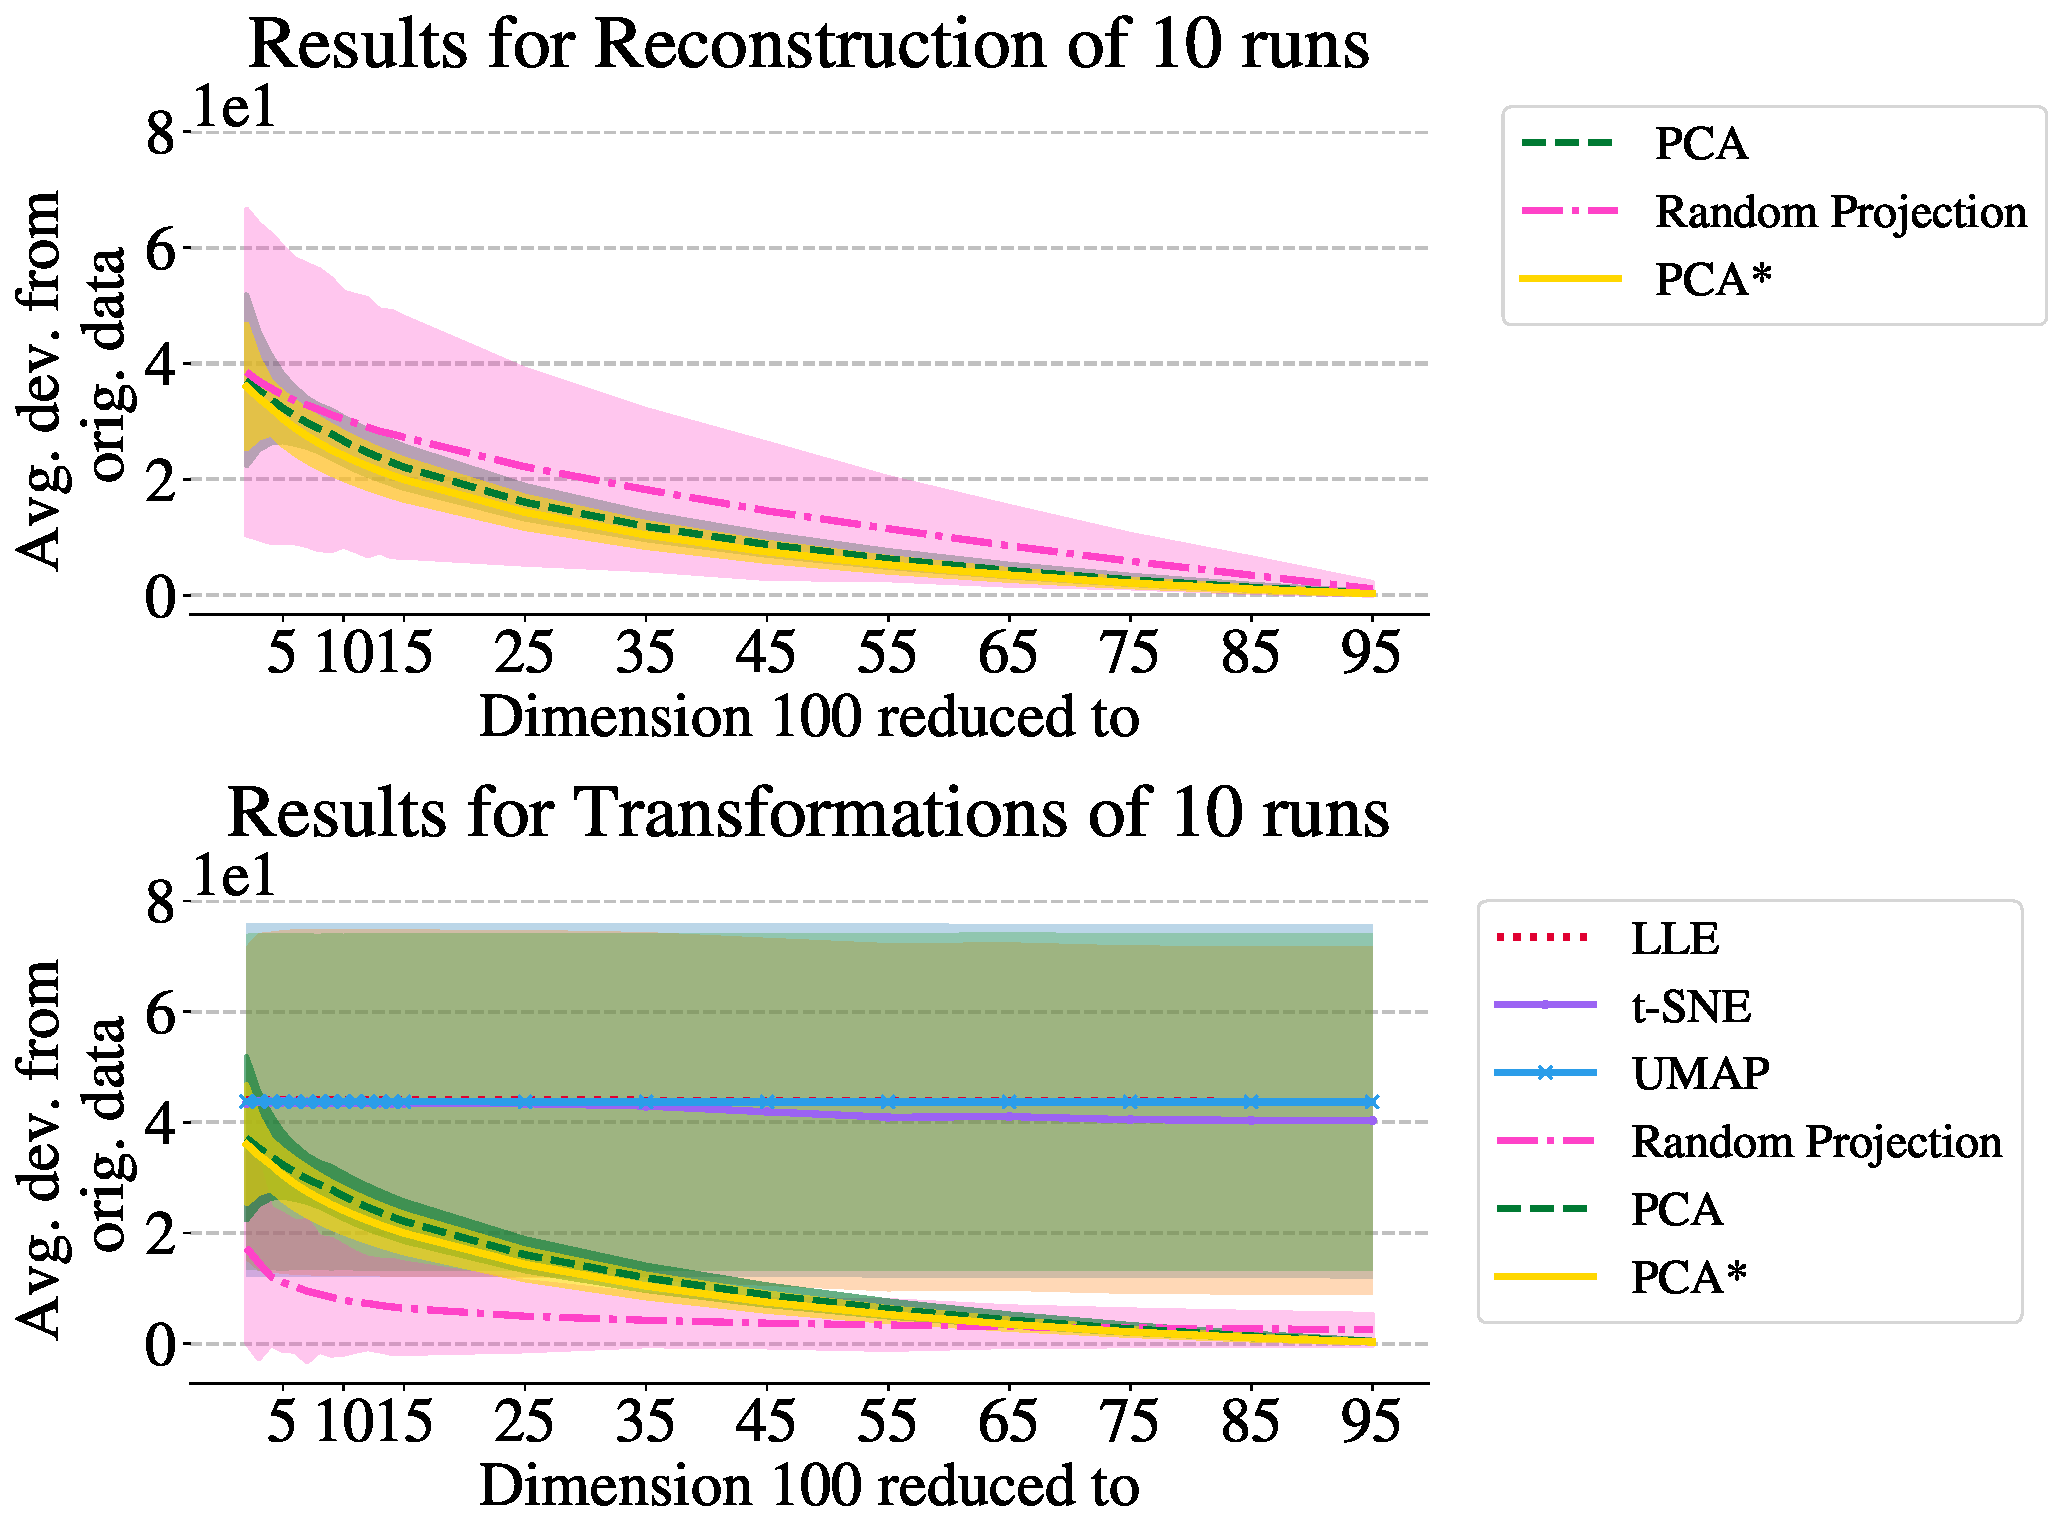
\includegraphics[width=7cm]{./images/multiple_runs/one_line/avg_dev_vs_dyn_low/5lines_100points_1neighbours_euclidean.pdf}}
    % \hfill
    \subfigure[Neighbour-Relation measure]{\includegraphics[width=7cm]{./images/multiple_runs/one_line/avg_dev_vs_dyn_low/5lines_100points_1neighbours_multiple_scalar_product.pdf}}
    \caption{Results for smoothly ordered data: increasing the number of dimensions of the lower-dimensional space}\label{fig:avg_dev_dyn_low_oneline}
\end{figure}

Comparing the results of the dimensionality reduction methods applied to smoothly ordered data, we observe that LLE, t-SNE and UMAP are again stable but with a lower variable than the ones on zigzag data, as shown in Figure~\ref{fig:avg_dev_dyn_low_oneline}.
This improvement may be attributed to the smoother data order, which is more akin to the spatial structure.
Similarly, the reconstruction of data transformed by random projection yields results comparable with PCA and PCA*.
However, concerning the transformed data, random projection outperforms PCA*.
PCA*s variance is nevertheless the smallest to all other compared techniques.
Moreover, it shows for both spaces improving results and measured with MNR, we see PCA* outperforming PCA and random projection for their reconstructed representation.

\begin{figure}[!htb]
    \subfigure[Neighbour-Distance Measure]{\includegraphics[width=7cm]{./images/multiple_runs/one_line/avg_dev_vs_dyn_low/5lines_100points_1neighbours_euclidean_cutk10.pdf}}
    % \hfill
    \subfigure[Neighbour-Relation measure]{\includegraphics[width=7cm]{./images/multiple_runs/one_line/avg_dev_vs_dyn_low/5lines_100points_1neighbours_multiple_scalar_product_cutk10.pdf}}
    \caption{Results for one-line data: increasing the number of dimensions between 2 and 10 for the lower-dimensional space}\label{fig:avg_dev_dyn_low_oneline_zoom}
\end{figure}

Zooming into the first 10 dimensions, we see in Figure~\ref{fig:avg_dev_dyn_low_oneline_zoom} PCA* displaying enhanced results compared to the other dimensionality reduction methods for both tested measures as well as for both reconstructed and transformed embeddings. 
In this case, the random projection transformed data maintains the averaged distances better in the mean.

\begin{figure}[!htb]
    \subfigure[Neighbour-Distance Measure]{\includegraphics[width=7cm]{./images/multiple_runs/sep_lines/avg_dev_vs_dyn_low/5lines_100points_1neighbours_euclidean.pdf}}
    \subfigure[Neighbour-Relation measure]{\includegraphics[width=7cm]{./images/multiple_runs/sep_lines/avg_dev_vs_dyn_low/5lines_100points_1neighbours_multiple_scalar_product.pdf}}
    \caption{Results for data in 5 separate lines: increasing the number of dimensions of the lower-dimensional space}\label{fig:avg_dev_dyn_low_seplines}
\end{figure}

These results are comparable to the outcomes of applying the dimensionality reduction methods to data in separate lines, as illustrated in Figure~\ref{fig:avg_dev_dyn_low_seplines}.
The performance of PCA* is overall enhanced, apart from the case of comparing respective distances between consecutive data points of the transformed data with the original data.
Here random projection outperforms with a higher variance.

\begin{figure}[!htb]
    \subfigure[Neighbour-Distance Measure]{\includegraphics[width=7cm]{./images/multiple_runs/sep_lines/avg_dev_vs_dyn_low/5lines_100points_1neighbours_euclidean_cutk10.pdf}}
    \subfigure[Neighbour-Relation measure]{\includegraphics[width=7cm]{./images/multiple_runs/sep_lines/avg_dev_vs_dyn_low/5lines_100points_1neighbours_multiple_scalar_product_cutk10.pdf}}
    \caption{Results for data in 5 separate lines: increasing the number of dimensions between 2 and 10 for the lower-dimensional space}\label{fig:avg_dev_dyn_low_seplines_zoom}
\end{figure}

Exploring a lower number of dimensions for each transformation, we see PCA* maintaining the order-based distances better than PCA, LLE, t-SNE and UMAP for the reconstruction and transformation measured with both measures ND and MNR.
Compared to random projection, we see PCA* having lower results when quantifying the distances and relations of consecutive data points in the order of the reconstructed data, as depicted in Figure~\ref{fig:avg_dev_dyn_low_seplines_zoom}.
In the case of transformed data, the representation of random projection maintains the pairwise distances computed with ND measure better overall, with a higher variance.
If we compare the results calculated by the MNR measure, we see PCA* keeping the relations between consecutive data points in dimensions lower than four better than random projection.
After that, random projection outperforms all of the other dimensionality reduction methods.

\begin{figure}[!htb]
    \subfigure[Zigzag data]{\includegraphics[width=4.6cm]{./images/multiple_runs/zigzag/avg_dev_vs_dyn_low/5lines_100points_1neighbours_dtw.pdf}}
    \subfigure[One-line data]{\includegraphics[width=4.6cm]{./images/multiple_runs/one_line/avg_dev_vs_dyn_low/5lines_100points_1neighbours_dtw.pdf}}
    \subfigure[Data in separate lines]{\includegraphics[width=4.6cm]{./images/multiple_runs/sep_lines/avg_dev_vs_dyn_low/5lines_100points_1neighbours_dtw.pdf}}
    \caption{Results for data in different orders measured with DTW} \label{fig:avg_dev_dyn_low_dtw}
\end{figure}

Figure \ref{fig:avg_dev_dyn_low_dtw} visualises the results for reconstructions of PCA*, PCA and random projection computed with DTW.
We see that similarly to the previous section, PCA and PCA* have comparable results for the reconstruction of zigzag data, whereas the reconstruction of data smoothly ordered or ordered in separate lines shows poorer results than PCA.
However, random projection does not keep the DTW distances as well as PCA and PCA*.

\FloatBarrier

\subsection{Exploration of Increasing Numbers of Neighbours} \label{subsec:increasing-neighb-synthetic}
As dimensionality reduction methods with the local-structure preserving property rely on the concept of nearest neighbours, we evaluate the effect of dimensionality reduction on the data with an increasing number of observed neighbours.
We first apply dimensionality reduction methods to the 100-dimensional data to reduce the dimensions to two.
We then measure the quality of the transformations for an increasing number of neighbours by quantifying how different the transformed data is compared to the original data.
% Therefore, we assess how the relationships between an increasing number of neighbours affect the original and the transformed data.
Thus this scenario helps us understand how well the dimensionality reduction method preserves the sequential structure within the data.
As our focus lies on order-based distance preservation, we define neighbours as data points which are close to each other in the sequential order of the data.
% We use the Neighbour-Distance measure (ND measure) as the measure to quantify the deviation of the distances of each neighbour within the original and the transformed space, and analogously the Multiple-Neighbour-Relation measure (MNR measure) for the relations.

In the following context, when we refer to observing $k$ neighbours, we are specifying that we are considering $k$ predecessors and $k$ successors that appear within the sequence.

\begin{figure}[!htb]
    \subfigure[Neighbour-Distance Measure]{\includegraphics[width=7cm]{./images/multiple_runs/zigzag/neighb_error/5lines_100points_5neighbours_euclidean.pdf}}
    \subfigure[Multiple-Neighbour-Relation Measure]{\includegraphics[width=7cm]{./images/multiple_runs/zigzag/neighb_error/5lines_100points_5neighbours_multiple_scalar_product.pdf}}
    \caption{Results for data in zigzag order: increasing the number of observed neighbours} \label{fig:num_neigh_zigzag}
\end{figure}

Comparing the average deviations for an increasing number of neighbours on zigzag data between its reconstructed and original data and respectively transformed representation with the original data, highlights PCA*'s ability to maintain the distances and relations to its predecessor and successor, see Figure~\ref{fig:num_neigh_zigzag}.
For more than two neighbours, the results of PCA and PCA* become more comparable.
Random projection, however, shows similar results to the other local structure-preserving methods LLE, t-SNE and UMAP.
Each of them performs stable for up to four neighbours and then increases in quality.

\begin{figure}[!htb]
    \subfigure[Neighbour-Distance Measure]{\includegraphics[width=7cm]{./images/multiple_runs/one_line/neighb_error/5lines_100points_5neighbours_euclidean.pdf}}
    \subfigure[Multiple-Neighbour-Relation Measure]{\includegraphics[width=7cm]{./images/multiple_runs/one_line/neighb_error/5lines_100points_5neighbours_multiple_scalar_product.pdf}}
    \caption{Results for smoothly ordered data: increasing the number of observed neighbours}\label{fig:num_neigh_oneline}
\end{figure}

Now, applying the same analysis to the data connected in a smooth line, we observe the means of PCA and PCA* being similar, as shown in Figure~\ref{fig:num_neigh_oneline}.
Random projection outperforms PCA* mean-wise in the lower-dimensional projection.
However, PCA* exhibits a much lower variance compared to the other methods included in the comparison.
When quantifying the results using the MNR measure, we notice a significant improvement for PCA* over PCA, the more neighbours we compare in the original dimensional space.
In the lower-dimensional embedding, the results of random projection are, compared to the other methods, strongly increasing, implying that random projection does not maintain the angular relations within the data as well.
This observation aligns with findings from previous experiments.

\begin{figure}[!htb]
    \subfigure[Neighbour-Distance Measure]{\includegraphics[width=7cm]{./images/multiple_runs/sep_lines/neighb_error/5lines_100points_5neighbours_euclidean.pdf}}
    \subfigure[Multiple-Neighbour-Relation Measure]{\includegraphics[width=7cm]{./images/multiple_runs/sep_lines/neighb_error/5lines_100points_5neighbours_multiple_scalar_product.pdf}}
    \caption{Results for data in separate lines: increasing the number of observed neighbours}\label{fig:num_neigh_seplines}
\end{figure}

Moving onto the analysis of dimensionality reduction methods applied to data ordered in separate lines, as illustrated in Figure~\ref{fig:num_neigh_seplines}.
In this scenario, we observe a consistently strong performance by PCA* relative to other dimensionality reduction methods for both measures, with one exception.
In the lower-dimensional representation, random projection excels at preserving the distances between consecutive points compared to PCA*, for example.
Nevertheless, when we examine the relations with the MNR measure, we once again notice that random projection struggles to maintain the connections between these data pairs effectively.

\FloatBarrier

\subsection{Analysis of Growing Numbers of Neighbours and Transformation Dimensions} \label{subsec:num_neigh_vs_dyn_low}

In this scenario, we apply dimensionality reduction methods to a 100-dimensional dataset.
We systematically increase the number of dimensions for the transformation while observing a growing number of neighbours.
The process involves reducing the dimensionality of the data and then comparing the average deviation in the relationships between nearby data points in both the original and transformed spaces. Essentially, this scenario combines elements from the second and third settings.
To quantify the results, we use the two quality measures defined in Section~\ref{quality-measures}: Neighbour-Distance measure (ND measure) and Multiple-Neighbour-Relation measure (MNR measure).

\begin{figure}[htb!]
    \includegraphics*[width= \textwidth]{images/multiple_runs/zigzag/dyn_low_dim_vs_num_neigh/euclidean/all_methods_10runs_5lines_100points_5neighbours.pdf}
    \caption{ND measure for zigzag data: Comparing the results of different dimensionality reduction methods for increasing numbers of neighbours and dimensionalities of the transformed space} \label{fig:dyn_low_dim_vs_num_neigh_zigzag}
\end{figure}

We begin by comparing the results of applying dimensionality reduction methods to zigzag-ordered data and quantifying them using the ND measure, as shown in figure \ref{fig:dyn_low_dim_vs_num_neigh_zigzag}.
In the higher-dimensional space, we observe that PCA and PCA* exhibit similar performance, with PCA* outperforming PCA when reducing the data to two dimensions and comparing the first predecessor and successor of each data point.
In contrast, random projection demonstrates poor results in the higher-dimensional space and marginally poorer performance in the lower-dimensional space than PCA* and PCA.
Thus, each of these methods keeps the distance to the nearest five neighbours comparably low, except from random projection in higher-dimensional space.
However, LLE, t-SNE, and UMAP encounter challenges in preserving the order-based distances within the data.
Due to their focus on local structure preservation, we see an improved result for comparing the results up to the fifth predecessor and successor.


\begin{figure}[htb!]
    \includegraphics*[width= \textwidth]{images/multiple_runs/zigzag/dyn_low_dim_vs_num_neigh/multiple_scalar_product/all_methods_10runs_5lines_100points_5neighbours.pdf}
    \caption{MNR measure for zigzag data: Comparing the results of different dimensionality reduction methods for increasing numbers of neighbours and dimensionalities of the transformed space} \label{fig:dyn_low_dim_vs_num_neigh_zigzag_scal}
\end{figure}

Similar to these results, PCA and PCA* produce roughly equal results for the MNR measure, but PCA* outperforms PCA for only one predecessor and successor while underperforming for up to three neighbours on both sides, as shown in Figure~\ref{fig:dyn_low_dim_vs_num_neigh_zigzag_scal}.
In higher dimensionality, the quality of results for random projection is poorer compared to PCA and PCA*.
Random projection, LLE, t-SNE and UMAP exhibit their local structure preservation effect, similar to the case before.
However, random projection starts with worse performance in lower dimensions for the transformations and shows improved performance for more than 55 dimensions. 
In contrast,  LLE, t-SNE and UMAP maintain consistently similar results across different dimensions.

\begin{figure}[htb!]
    \includegraphics*[width= \textwidth]{images/multiple_runs/one_line/dyn_low_dim_vs_num_neigh/euclidean/all_methods_10runs_5lines_100points_5neighbours.pdf}
    \caption{ND measure for smoothly ordered data: Comparing the results of different dimensionality reduction methods for increasing numbers of neighbours and dimensionalities of the transformed space} \label{fig:dyn_low_dim_vs_num_neigh_oneline}
\end{figure}

Figure \ref{fig:dyn_low_dim_vs_num_neigh_oneline} displays the performance of dimensionality reduction methods applied to smoothly ordered data, with results quantified using the ND measure.
We see again that PCA and PCA* yield similar outcomes, with PCA* exhibiting a slight advantage, particularly in lower dimensions.
On the other hand, random projection performs worse in its reconstructed form but excels in lower-dimensional settings compared to PCA, PCA*, LLE, t-SNE, and UMAP.
In the context of smoothly ordered data, LLE, t-SNE, and UMAP demonstrate poor results in preserving distances for various numbers of neighbours.


\begin{figure}[htb!]
    \includegraphics*[width= \textwidth]{images/multiple_runs/one_line/dyn_low_dim_vs_num_neigh/multiple_scalar_product/all_methods_10runs_5lines_100points_5neighbours.pdf}
    \caption{MNR measure for smoothly ordered data: Comparing the results of different dimensionality reduction methods for increasing numbers of neighbours and dimensionalities of the transformed space} \label{fig:dyn_low_dim_vs_num_neigh_oneline_scal}
\end{figure}

Assessing the quality of dimensionality reduction techniques using the MNR measure on smoothly ordered data reveals slightly better results for PCA* compared to PCA and random projection in higher dimensionality settings.
However, on transformed dimensionality, the result of random projection slightly outperforms PCA*.
In contrast, LLE, t-SNE, and UMAP consistently produce similar results across different dimensions and numbers of neighbours, as shown in Figure~\ref{fig:dyn_low_dim_vs_num_neigh_oneline_scal}.

\begin{figure}[htb!]
    \includegraphics*[width= \textwidth]{images/multiple_runs/sep_lines/dyn_low_dim_vs_num_neigh/euclidean/all_methods_10runs_5lines_100points_5neighbours.pdf}
    \caption{ND measure for data in separate lines: Comparing the results of different dimensionality reduction methods for increasing numbers of neighbours and dimensionalities of the transformed space} \label{fig:dyn_low_dim_vs_num_neigh_seplines}
\end{figure}

Similarly, the results for dimensionality reduction methods applied to data ordered on separate lines, show for PCA and PCA* similar results, with PCA* showing slight improvements, particularly when considering the first neighbours and lower dimensions.
Random projection, on the other hand, performs slightly worse than PCA and PCA* in the reconstructed embedding but surpasses them in the transformed representation.
In contrast, LLE, t-SNE, and UMAP consistently underperform when compared to PCA, PCA*, and random projection, as depicted in Figure~\ref{fig:dyn_low_dim_vs_num_neigh_seplines}.

\begin{figure}[htb!]
    \includegraphics*[width= \textwidth]{images/multiple_runs/sep_lines/dyn_low_dim_vs_num_neigh/multiple_scalar_product/all_methods_10runs_5lines_100points_5neighbours.pdf}
    \caption{MNR measure for data in separate lines: Comparing the results of different dimensionality reduction methods for increasing numbers of neighbours and dimensionalities of the transformed space} \label{fig:dyn_low_dim_vs_num_neigh_seplines_scal}
\end{figure}

Similar to the previous figures, Figure~\ref{fig:dyn_low_dim_vs_num_neigh_seplines_scal} reveals a marginal improvement for PCA* for the reconstructed data when compared to PCA and random projection.
PCA and random projection exhibit similar reconstruction quality. 
When comparing the transformations, we see random projection outperforming PCA*.
LLE, t-SNE, and UMAP consistently produce poorer outcomes compared to PCA.

\FloatBarrier

\subsection{Number of Lines Versus the Number of Neighbours}
To explore the impact of data complexity on the performance of dimensionality reduction methods, we generate datasets comprising 100-dimensional data points organised on a gradually increasing number of lines.
As the number of lines increases, the data's complexity also grows, allowing us to examine how different dimensionality reduction methods cope with varying levels of data intricacy.
We then apply various dimensionality reduction techniques to these datasets and assess their performance using the quality measures outlined in Section~\ref{quality-measures}:  Neighbour-Distance (ND) and Multiple-Neighbour-Relation (MNR).
Additionally, we analyze the results for different numbers of neighbours.
This experimental setup enables us to identify parameter combinations that provide insights into which dimensionality reduction method best preserves order-based distances and relations for an increasing number of neighbours in increasingly complex scenarios.

\begin{figure}[htb!]
    \includegraphics[width=\textwidth]{./images/multiple_runs/zigzag/num_lines_vs_num_neigh/euclidean/all_methods_10runs_10lines_100points_5neighbours.pdf}
    \caption{Zigzag data with ND measure: comparing the results of different dimensionality reduction methods for varying numbers of neighbours and numbers of lines} \label{fig:num_neigh_vs_num_lines_zigzag}
\end{figure}

We begin our analysis by examining the results of dimensionality reduction techniques applied to zigzag data using the ND measure.
The results are visualised in Figure~\ref{fig:num_neigh_vs_num_lines_zigzag}.
It becomes evident that PCA* demonstrates superior performance in preserving distances between each data point and its predecessor and successor when compared to PCA, random projection as well as LLE, t-SNE, and UMAP.
Apart from this, PCA* has a similar result to PCA.
Random projection struggles with order-based distance preservation in the reconstructed space but displays similar results to PCA in its transformation.
Additionally, Figure~\ref{fig:num_neigh_vs_num_lines_zigzag} illustrates that t-SNE yields better results than both LLE and UMAP but remains unable to match the order-based distance preservation achieved by PCA and PCA*. 
This observation aligns with the local structure-preserving nature of these techniques, as they aim to maintain distances that reflect the local context.


\begin{figure}[htb!]
    \includegraphics[width=\textwidth]{./images/multiple_runs/zigzag/num_lines_vs_num_neigh/multiple_scalar_product/all_methods_10runs_10lines_100points_5neighbours.pdf}
    \caption{Zigzag data with MNR measure: comparing the results of different dimensionality reduction methods for varying numbers of neighbours and numbers of lines}\label{fig:num_neigh_vs_num_lines_zigzag_scal}
\end{figure}

Figure \ref{fig:num_neigh_vs_num_lines_zigzag_scal} presents results for the dimensionality reduction methods to zigzag data, using the MNR measure to assess order-based relation preservation across varying numbers of neighbours and lines in both the reconstructed and transformed representations.
PCA* outperforms PCA in retaining relationships with the first neighbours on the order for both directions, while exhibiting similar overall performance.
In contrast, random projection fares less favourably, showing reduced preservation of order-based distances in both higher and lower-dimensional representations compared to PCA and PCA*. 
Random projection, LLE, t-SNE, and UMAP perform well when data is distributed along a single line but struggle to maintain relationships in the presence of complex zigzag patterns.
This is consistent with their strengths in preserving local distances.

\begin{figure}[htb!]
    \includegraphics[width=\textwidth]{./images/multiple_runs/one_line/num_lines_vs_num_neigh/euclidean/all_methods_10runs_10lines_100points_5neighbours.pdf}
    \caption{Smoothly ordered data with ND measure: comparing the results of different dimensionality reduction methods for varying numbers of neighbours and numbers of lines} \label{fig:num_neigh_vs_num_lines_oneline}
\end{figure}

Applying our analysis to data ordered connected with a smooth line, we observe generally better results for PCA* when there are more than two lines, as shown in Figure~\ref{fig:num_neigh_vs_num_lines_oneline}.
PCA outperforms PCA* for one and two lines.
However, as the number of lines increases, PCAs performance declines.
In contrast, random projection maintains the order-based distances less effectively in its reconstructed form but excels in its lower-dimensional embedding, a pattern consistent with other settings.
LLE, t-SNE, and UMAP exhibit poor performance in preserving order-based distances as the number of lines and neighbours grows.

\begin{figure}[htb!]
    \includegraphics[width=\textwidth]{./images/multiple_runs/one_line/num_lines_vs_num_neigh/multiple_scalar_product/all_methods_10runs_10lines_100points_5neighbours.pdf}
    \caption{Smoothly ordered data with MNR measure: comparing the results of different dimensionality reduction methods for varying numbers of neighbours and numbers of lines}\label{fig:num_neigh_vs_num_lines_oneline_scal}
\end{figure}

Figure \ref{fig:num_neigh_vs_num_lines_oneline_scal} reveals a significant difference between PCA, PCA* and random projection.
While random projection's results are roughly comparable to PCA* in the higher-dimensional space, its respective transformation shows poor results compared to PCA and PCA*.
Comparing the results of PCA and PCA*, we see that PCA* outperforms PCA for one line and more neighbours but resembles more and more the result of PCA as the number of lines and neighbours increases.
Similarly, LLE, t-SNE and UMAP also perform well in this experiment and are thereby comparable to PCA*.

\begin{figure}[htb!]
    \includegraphics[width=\textwidth]{./images/multiple_runs/sep_lines/num_lines_vs_num_neigh/euclidean/all_methods_10runs_10lines_100points_5neighbours.pdf}
    \caption{Separate lines data with ND measure: comparing the results of different dimensionality reduction methods for varying numbers of neighbours and numbers of lines} \label{fig:num_neigh_vs_num_lines_seplines}
\end{figure}

Similar to the results of ND measure on data which is connected with one line, the results of applying various dimensionality reduction methods on data which is ordered on separate lines, show that PCA* generally better maintains the order-based distances than PCA, see Figure~\ref{fig:num_neigh_vs_num_lines_seplines}, except from data being in only one line.
Random projection, as previously, exhibits worse results in the original space with its reconstructed data, but in the lower-dimensional space, it performs well.
LLE, t-SNE, and UMAP also display equally poor results compared to PCA, PCA*, and random projection.

\begin{figure}[htb!]
    \includegraphics[width=\textwidth]{./images/multiple_runs/sep_lines/num_lines_vs_num_neigh/multiple_scalar_product/all_methods_10runs_10lines_100points_5neighbours.pdf}
    \caption{Separate lines data with MNR measure: comparing the results of different dimensionality reduction methods for varying numbers of neighbours and numbers of lines}\label{fig:num_neigh_vs_num_lines_seplines_scal}
\end{figure}

For the same experimental setting but using the MNR measure, we observe marginally better results for PCA* compared to PCA for 3 or more lines, with PCA performing better on one and two lines, as seen in Figure~\ref{fig:num_neigh_vs_num_lines_seplines_scal}.
Random projection demonstrates similar results in the original space to PCA but performs better for one or two lines.
In the transformed space, it exhibits poor results, as it fails to retain the relations between connections as effectively as PCA and PCA*. 
Additionally, each of the tested methods performs slightly better for a lower number of neighbours.


\FloatBarrier

\section{Evaluation on Real-World and Simulated Data} \label{real-world-experiments}
Due to noise, missing data points or outliers, real-world and simulated data may often be more complex than the generated data.
In this section, we expand our analysis to three real-world datasets: Russell2000, MTS Flights and air pollution data in Japan.
% Russell2000 and the air pollution data are real-world data, while the MTS Flight data is a simulated dataset containing information about 10 flights.
These datasets vary in dimensionality, ranging from very high dimensional (over 1000 dimensions) to lower dimensions (29).
For this analysis, we will primarily focus on using PCA* as it has shown promising results in previous experiments, outperforming both PCA and the variants of CPCA.  

\subsection{Expanding the Dimensionality of the Transformation}
\FloatBarrier
In the following, the average deviation from each reconstruction and transformation of real-world and simulated data in comparison to the original data.
Average deviation is defined as the mean of all summed differences between each data point and its predecessor and successor.
As we have seen in Subsection~\ref{sec:avg_dev_vs_dyn_low_dims}, the results of LLE, t-SNE and UMAP remained constant.
Therefore, we omit these techniques in this experiment.


In Figure~\ref{fig:avg_dev_vs_low_dim-russell}, we observe a notable difference in the variances and mean values between random projection, PCA and PCA*.
Random projection exhibits a significant overall spread, indicating a wider range of variability in the results.
Both embeddings of random projection diverge much more on average from the original data than the results of PCA and PCA*.
When we focus on the comparison between PCA and PCA*, we observe that PCA* performs marginally better than PCA.
This implies in both terms of mean and variance suggesting that PCA* maintains slightly better pairwise distances within the data.
On the other hand, comparing the results of the methods with the NR measure we see PCA* demonstrating improvement over PCA in ranges 2 to roughly 480.
Beyond this range, PCA continues to excel in maintaining relationships among data points.
In all scenarios within this experiment, it is evident that both PCA and PCA* exhibit a sharp improvement as the dimensionality increases up to 400.
This is due to the dataset having more dimensions than data points and consisting of 504 observations, enabling PCA and PCA* to effectively preserve order-based distances well.
Interestingly, the outcome of random projections only exhibits a gradual decrease, even when transforming to a higher dimension than the dataset contains data points.

When applying the dimensionality reduction methods to the MTS dataset, we observe remarkably high performances achieved by both PCA and PCA*.
The exceptional results may be due to the inherent limitations of this dataset, see the paragraph on real-world and simulated data in Section~\ref{real-world-data}.
Notably, PCA* constantly outperforms PCA, suggesting a slightly better preservation for both distances and relations among data points.
In contrast, random projection exhibits consistently suboptimal results across all dimensions to which the data was reduced, as illustrated in Figure~\ref{fig:avg_dev_vs_low_dim-flights}.

When we transform the air pollution data to an increasing number of dimensions, we observe that random projection consistently produces poor results when comparing the relations of its reconstructed representation to the original data, see Figure~\ref{fig:avg_dev_vs_low_dim-air}.
However, when comparing the transformed data, we find that it yields better results than PCA and PCA*.
This scenario resembles the setting in which we applied the dimensionality reduction methods to smoothly ordered data.
This similarity suggests that this dataset may exhibit lower fluctuations.
Across all settings, PCA* consistently outperforms PCA in preserving relationships and distances between consecutive data points.

\begin{figure}[htb!]
    \includegraphics[width=7cm]{./images/real-world/russell2000_stock/avg_dev_vs_dyn_low/reconstructed_1lines_504points_euclidean.pdf}
    \includegraphics[width=7cm]{./images/real-world/russell2000_stock/avg_dev_vs_dyn_low/reconstructed_1lines_504points_multiple_scalar_product.pdf}
    \includegraphics[width=7cm]{./images/real-world/russell2000_stock/avg_dev_vs_dyn_low/transformed_1lines_504points_euclidean.pdf}
    \includegraphics[width=7cm]{./images/real-world/russell2000_stock/avg_dev_vs_dyn_low/transformed_1lines_504points_multiple_scalar_product.pdf}
    \caption{Russell2000 data: Comparing the results of different dimensionality reduction methods for an increasing number of transformation dimensionality} \label{fig:avg_dev_vs_low_dim-russell}
\end{figure}

\begin{figure}[htb!]
    \includegraphics[width=7cm]{./images/real-world/flights/avg_dev_vs_dyn_low/reconstructed_10lines_4660points_euclidean.pdf}
    \includegraphics[width=7cm]{./images/real-world/flights/avg_dev_vs_dyn_low/reconstructed_10lines_4660points_multiple_scalar_product.pdf}
    \includegraphics[width=7cm]{./images/real-world/flights/avg_dev_vs_dyn_low/transformed_10lines_4660points_euclidean.pdf}
    \includegraphics[width=7cm]{./images/real-world/flights/avg_dev_vs_dyn_low/transformed_10lines_4660points_multiple_scalar_product.pdf}
    \caption{MTS flights data: Comparing the results of different dimensionality reduction methods for an increasing number of transformation dimensionality. Variance is omitted due to visibility reasons.} \label{fig:avg_dev_vs_low_dim-flights}
\end{figure}
\begin{figure}
    \includegraphics[width=7cm]{./images/real-world/air_pollution/avg_dev_vs_dyn_low/reconstructed_1lines_4380points_euclidean.pdf}
    \includegraphics[width=7cm]{./images/real-world/air_pollution/avg_dev_vs_dyn_low/reconstructed_1lines_4380points_multiple_scalar_product.pdf}
    \includegraphics[width=7cm]{./images/real-world/air_pollution/avg_dev_vs_dyn_low/transformed_1lines_4380points_euclidean.pdf}
    \includegraphics[width=7cm]{./images/real-world/air_pollution/avg_dev_vs_dyn_low/transformed_1lines_4380points_multiple_scalar_product.pdf}
    \caption{Air-pollution data: Comparing the results of different dimensionality reduction methods for an increasing number of transformation dimensionality}\label{fig:avg_dev_vs_low_dim-air}
\end{figure}



\FloatBarrier

\subsection{Exploration of Increasing Numbers of Neighbours} \label{subsec:increasing-neighb-real}


\FloatBarrier
Similar to Subsection~\ref{subsec:increasing-neighb-synthetic}, we now investigate how PCA, PCA*, and random projection reduce the dimensionality of real-world data from their original high dimensionalities to 2 dimensions.
We then quantify, for an increasing number of neighbours in each sequence direction, how effectively these methods preserve both distances and relations.
We use the Neighbour-Distance (ND) to measure how well distances are kept and the Multiple-Neighbour Relation (MNR) for assessing the preservation of relationships in this analysis.
These measures are described in Section~\ref{quality-measures}. 

Analogously to the separate lines, we measure the distances and relations within each flight of the MTS-flights data separately.


\begin{figure} [htb!]
    \includegraphics[width=7cm]{./images/real-world/russell2000_stock/num_neigh/transformed_1lines_504points_euclidean.pdf}
    \includegraphics[width=7cm]{./images/real-world/russell2000_stock/num_neigh/transformed_1lines_504points_multiple_scalar_product.pdf}
    \caption{Russell2000 data: Comparing the results of different dimensionality reduction methods for varying numbers of neighbours} \label{fig:num_neigh-russell}
\end{figure}
\begin{figure}[htb!]
    \includegraphics[width=7cm]{./images/real-world/flights/num_neigh/transformed_10lines_4660points_euclidean.pdf}
    \includegraphics[width=7cm]{./images/real-world/flights/num_neigh/transformed_10lines_4660points_multiple_scalar_product.pdf}
    \caption{MTS flights: Comparing the results of different dimensionality reduction methods for varying numbers of neighbours}\label{fig:num_neigh-flights}
\end{figure}

When applying dimensionality reduction methods to both the Russell2000 and the MTS flight data, we observe similar outcomes, as depicted in Figure~\ref{fig:num_neigh-russell} and Figure~\ref{fig:num_neigh-flights}.
Notably, random projection exhibits poor performance in preserving distances and relations between different numbers of successors and predecessors, in contrast to PCA and PCA*.
Interestingly, LLE, t-SNE and UMAP yield even worse results than random projection.
However, PCA* demonstrates a marginal improvement over PCA in preserving distances and significantly outperforms both PCA and other methods in maintaining relations within the data.

\begin{figure}
    \includegraphics[width=7cm]{./images/real-world/air_pollution/num_neigh/transformed_1lines_4380points_euclidean.pdf}
    \includegraphics[width=7cm]{./images/real-world/air_pollution/num_neigh/transformed_1lines_4380points_multiple_scalar_product.pdf}
    \caption{Air-pollution data: Comparing the results of different dimensionality reduction methods for varying numbers of neighbours}
    \label{fig:num_neigh-air}
\end{figure}

On the air pollution data, every dimensionality reduction method maintains the distances within the data similarly, apart from the lower-dimensional transformation of random projection, which keeps distances almost constantly low for all increasing neighbours, as illustrated in Figure~\ref{fig:num_neigh-air}.
On the other hand, comparing the relations within both embeddings with the relations within the original data shows that PCA* is the best dimensionality reduction method and random projection the worst.

\FloatBarrier
\subsection{Analysis of Growing Numbers of Neighbours and Transformation Dimensions}

Analogous to previous subsections, we explore the effects of changing two key parameters in the transformation and reconstruction evaluation: the number of successors and predecessors, and the number of dimensions used to transform the data.
In every dimensionality reduction step, we quantify the order-based distance and relation preservation for a growing number of neighbours on the sequence with the Neighbour-Distance (ND) and Multiple-Neighbour-Relation (MNR) measure compared to the distances and relations in the original data, see Section~\ref{quality-measures}.
By comparing the results with the original data, we gain insights into the trade-offs between order-based distance and relation preservation when applying dimensionality reduction techniques to sequential data.


Comparing the quality of the results of dimensionality reduction methods that transformed the Russell2000 data to an increasing number of dimensions juxtaposed to the number of neighbours examined, we see similar results measured with ND and MNR measures, see Figure~\ref{fig:num_neigh_vs_dyn_low-eucl-russel} and \ref{fig:num_neigh_vs_dyn_low-mscal-russel}.
PCA* marginally improves the order-based distances and relations within the data of PCA, see figures \ref{fig:num_neigh_vs_dyn_low-eucl-russel_zoom} and \ref{fig:num_neigh_vs_dyn_low-mscal-russel_zoom}.

Analogously to previous experiments, random projection maintains order-based distances and relations better than its reconstructed counterpart.
LLE, t-SNE and UMAP are comparably suboptimal, as they maintain the distances and relations to the first neighbours better and then decrease in quality the more neighbours we observe.

When we apply dimensionality reduction methods to the MTS flight data, we observe similar results for both PCA and PCA* when assessed with ND and MNR measures, as illustrated in figures \ref{fig:num_neigh_vs_dyn_low-eucl-flights} and \ref{fig:num_neigh_vs_dyn_low-mscal-flights}.
For a more detailed comparison between PCA and PCA* figures \ref{fig:num_neigh_vs_dyn_low-eucl-flights-zoom} and \ref{fig:num_neigh_vs_dyn_low-mscal-flights-zoom} depict their results with a separate scale.
With the ND measure, both PCA and PCA* perform similarly.
However, when using the MNR measure, we observe that PCA* outperforms PCA, especially for transformations to two dimensions.
The reconstruction of random projects underperformed compared to PCA and PCA*.
However, its transformations, while not as good as those of PCA and PCA*, are still better than the results achieved by LLE, t-SNE, and UMAP.
It's worth noting that t-SNE encountered issues with the flight dataset, particularly when the dataset contained rows with a standard deviation of zero. 
This limitation highlights one of the disadvantages of t-SNE, as other dimensionality reduction methods were able to handle this dataset successfully.

Figure \ref{fig:num_neigh_vs_dyn_low-eucl-air} shows comparable results for PCA and PCA*, with PCA* performing slightly better for the first two neighbours. 
The overall pattern is consistent with the observations made in the Russell2000 data scenario.

PCA* outperforms all other dimensionality reduction methods in all settings when applied to the air pollution data assessed with the MNR measure, see Figure~\ref{fig:num_neigh_vs_dyn_low-mscal-air}.


\begin{figure}
    \includegraphics[width = \textwidth]{images/real-world/russell2000_stock/dyn_low_dim_vs_num_neigh/euclidean/all_methods_1runs_1lines_504points_5neighbours.pdf}
    \caption{Neighbour-Distance measure on Russell2000 data: Comparing the results of different dimensionality reduction methods for increasing numbers of neighbours and dimensionality of the transformed space with the original data} \label{fig:num_neigh_vs_dyn_low-eucl-russel}
\end{figure}


\begin{figure}
    \includegraphics[width = \textwidth]{images/real-world/russell2000_stock/dyn_low_dim_vs_num_neigh/multiple_scalar_product/all_methods_1runs_1lines_504points_5neighbours.pdf}
    \caption{Multiple-Neighbour-Relation measure on Russell2000 data: Comparing the results of different dimensionality reduction methods for increasing numbers of neighbours and dimensionality of the transformed space with the original data} \label{fig:num_neigh_vs_dyn_low-mscal-russel}
\end{figure}

\begin{figure}
    \subfigure[Neighbour-Distance measure on Russell2000 data]{\includegraphics[width = \textwidth /2]{images/real-world/russell2000_stock/dyn_low_dim_vs_num_neigh/euclidean/onlypcas1runs_1lines_504points_5neighbours.pdf} \label{fig:num_neigh_vs_dyn_low-eucl-russel_zoom}}
    \hfill
    \subfigure[Neighbour-Distance measure on MTS flight data]{\includegraphics[width = \textwidth/2]{images/real-world/flights/dyn_low_dim_vs_num_neigh/euclidean/onlypcas1runs_10lines_4660points_5neighbours.pdf} \label{fig:num_neigh_vs_dyn_low-eucl-flights-zoom}}
    \hfill
    \subfigure[Multiple-Neighbour-Relation measure on Russell2000 data]{\includegraphics[width = \textwidth /2]{images/real-world/russell2000_stock/dyn_low_dim_vs_num_neigh/multiple_scalar_product/onlypcas1runs_1lines_504points_5neighbours.pdf} \label{fig:num_neigh_vs_dyn_low-mscal-russel_zoom}}
    \hfill
    \subfigure[Multiple-Neighbour-Relation measure on MTS flight data]{\includegraphics[width = \textwidth/2]{images/real-world/flights/dyn_low_dim_vs_num_neigh/multiple_scalar_product/onlypcas1runs_10lines_4660points_5neighbours.pdf} \label{fig:num_neigh_vs_dyn_low-mscal-flights-zoom}}
    \hfill
    \caption{Comparing the results of PCA and PCA* separately for increasing numbers of neighbours and dimensionality of the transformed space with the original data}
\end{figure}

\begin{figure}
    \includegraphics[width = \textwidth]{images/real-world/flights/dyn_low_dim_vs_num_neigh/euclidean/all_methods_1runs_10lines_4660points_5neighbours.pdf}
    \caption{Neighbour-Distance measure on MTS flights data: Comparing the results of different dimensionality reduction methods for increasing numbers of neighbours and dimensionality of the transformed space with the original data} \label{fig:num_neigh_vs_dyn_low-eucl-flights}
\end{figure}


\begin{figure}
    \includegraphics[width = \textwidth]{images/real-world/flights/dyn_low_dim_vs_num_neigh/multiple_scalar_product/all_methods_1runs_10lines_4660points_5neighbours.pdf}
    \caption{Multiple-Neighbour-Relation measure on MTS flights data: Comparing the results of different dimensionality reduction methods for increasing numbers of neighbours and dimensionality of the transformed space with the original data} \label{fig:num_neigh_vs_dyn_low-mscal-flights}
\end{figure}


\begin{figure}
    \includegraphics[width = \textwidth]{images/real-world/air_pollution/dyn_low_dim_vs_num_neigh/euclidean/all_methods_1runs_1lines_4380points_5neighbours.pdf}
    \caption{Neighbour-Distance measure on air-pollution data: Comparing the results of different dimensionality reduction methods for increasing numbers of neighbours and dimensionality of the transformed space with the original data} \label{fig:num_neigh_vs_dyn_low-eucl-air}
\end{figure}


\begin{figure}
    \includegraphics[width = \textwidth]{images/real-world/air_pollution/dyn_low_dim_vs_num_neigh/multiple_scalar_product/all_methods_1runs_1lines_4380points_5neighbours.pdf}
    \caption{Multiple-Neighbour-Relation measure on air-pollution data: Comparing the results of different dimensionality reduction methods for increasing numbers of neighbours and dimensionality of the transformed space with the original data}
    \label{fig:num_neigh_vs_dyn_low-mscal-air}
\end{figure}


\FloatBarrier
\section{Limitations of Experiments}
In our research, we introduce a new setting focused on order-based distance preservation.
It is important to note that as this field is new and broad, our experiments represent only a subset of the possible scenarios that can be tested in this setting.

Furthermore, we acknowledge that the toy examples used in our experiments have limitations.
Specifically, they are designed to begin in a relatively simplified setting: consisting of 5 lines, each containing 100 data points.

It is also worth highlighting that in the real world, data may not always exhibit the same patterns as our toy example.
For instance, the strict zigzag ordering or the smooth ordering in our experiments may not accurately reflect the complexity and diversity of real-world data distributions.
They were used to simulate extreme orders like zigzag data simulating scenarios with high fluctuations, whereas smoothly ordered data represented data, which consists of the same data points, but without the rapid variations.

We also conducted tests on three real-world datasets.
These datasets used to evaluate our methods exhibited diverse characteristics, like varying in terms of dimensionality.
Furthermore, these datasets also had a varying number of observations, indicating different sample sizes.
Additionally, one of the datasets was composed of multiple time series data, which were all measured separately.
While this provides valuable insights, we recognize that the diversity of real-world data is vast, and these three datasets are only a small part of what exists.
Nevertheless, they offer a promising outlook for the applicability of our methods in more complex and varied scenarios.

In the case of CPCA, where we augmented the data with vectors as the imaginary part to account for the sequential information, it is important to note that certain challenges arise.
These challenges become evident when dealing with consecutive non-unique data points, as adding a 0-vector to the data may signal the end of a sequence.
Given that our approach allows for the presence of multiple sequences with the data, handling such cases requires careful consideration and adaptation of the CPCA techniques.

\section{Experimental Results}
In the series of experiments, we explored dimensionality reduction techniques, with a particular focus on order-based distance preservation.
Our investigations covered a spectrum of datasets, including synthetic and real-world data, of which the data varied in order and complexity.
The primary focus was to assess the performance of PCA* and the variants of CPCA in terms of their ability to preserve order-based distances and relationships within the data.

Our initial experiments involved synthetic data, which allowed us to control the data's characteristics.
We discovered that all variants of CPCA maintained the distances and relations suboptimal in comparison to PCA.
PCA on data with Ids performed comparably to PCA.
In our second experiment, we compared PCA* with various other dimensionality reduction methods.
We saw that PCA* exhibited consistently a good preservation for data with high fluctuations, whereas the lower dimensional representation of random projection on smoothly ordered data and data in separate lines (because it did not fluctuate as much) maintained exceptionally well the compared distances.
In contrast, its reconstruction is poor compared to the reconstructions of PCA* and PCA.

We applied our dimensionality reduction methods to real-world datasets, including financial data from the Russell2000, flight data from NASA MTS dataset and data on air pollution in Japan.
Here, too PCA* emerged as a robust performer, consistently outshining PCA in preserving relationships and distances between consecutive data points.
Random projection, although stable, lagged behind in terms of maintaining these order-based characteristics, apart from applying it to the air pollution data, where similarly to the smoothly ordered data, its transformation kept more order-based distances.


\chapter{Future Work} \label{future-work}
As the results of our experiments lay a foundation for future explorations in the field of dimensionality reduction and order-based distance preservation, we give some suggestions on what we believe PCA* and order-based distance preservation, in general, have the potential to enhance various data analysis tasks.

\paragraph*{Clustering}
PCA can be used in clustering applications, see \cite{pca-clustering}.
Our experiments have shown the promise of order-based distance preservation of PCA*. 
Future research may apply PCA* specifically for clustering tasks, where maintaining the intrinsic sequential order of data can be critical for effective clustering.

\paragraph{NLP and Text Analysis}
In the realm of Natural Language Processing (NLP), sentences are often represented as vectors \cite{nlp-sentences}.
Given that sentences inherently possess sequential order, the application of order-based distance preservation techniques holds the potential to enhance the accuracy and interpretability of NLP models.

\paragraph{Multiple Sequential Orders}
While our experiments focused on data with a single clear order, real-world scenarios often involve multiple orders within the same dataset.
For example, molecular dynamics or pixel data, where both structural and temporal orders coexist.
Future investigations may extend PCA* to accommodate and preserve these multiple orders effectively.

\paragraph{Partially Ordered Data}
We have primarily focused on data which is totally-ordered.
In future work, it is interesting to investigate the application of PCA* to data that is not linearly ordered but exhibits partial order, such as a hierarchy or graphs.
This exploration can give insight into how our order-based distance-preserving technique performs in scenarios where the data's structure is more complex and includes branches.
Therefore, testing PCA* on this scenario can provide more information about its versatility and effectiveness on a broader range of datasets.

\paragraph{Variable-Length Data}
Analysing the data with multiple sequences of varying lengths poses an interesting challenge.
We primarily focus in this work on equally long sequences, but as the MTS data shows, real-world data may not always be so similar.

\paragraph{Further Explorations for CPCA}
While order-based distance preservation is not the primary focus for the variants of CPCA, there may be a specialised use case where its incorporation may be useful.
Future research may uncover these applications and refine the methods for this scenario.

\paragraph{Order-Based Distance Preservation in Local Structure Preserving Methods}
As LLE, for example, employs the $k$-nearest neighbour algorithm, to find the spatially nearest neighbours of each point, it would be interesting to explore its adaptation to aiming for order-based distance preservation.
Here we would not be taking the $k$-nearest neighbours in the space but the sequential $k$-nearest neighbours.
This adaptation could lead to a representation of data which maintains the inherent order better than LLE currently.


\chapter{Conclusion} \label{conclusion}
In this thesis, we investigate dimensionality reduction methods applied to ordered data.
We introduce and analyse variants of PCA tailored to ordered data, including PCA with Ids, Complex PCA on ordered data and PCA*.

Our experiments, conducted with synthetic and real-world datasets, provide valuable insights into the performance of these techniques.
We explore the impact of various aspects, like the increasing number of dimensionality or a growing number of observed neighbours.

Overall, our experiments provide evidence that PCA* is a valuable tool for dimensionality reduction, particularly when order-based distances and relationships need to be preserved in a dataset where the order shows high variability.
% While random projection and other conventional techniques have their strengths, PCA* stands out for preserving order-based distances.
However, the choice of method should be driven by the specific goals and characteristics of the data at hand.
PCA* offers a valuable alternative when order-based information is crucial.

In future work, it is essential to further explore the generalisability of PCA*.
For instance, the extension of PCA* to multiple sequential orders or the application on a partially ordered dataset is intriguing for future investigations. 

\appendix
\chapter{Technical Details on Experiments}
\begin{table}[htb!]
    \begin{tabular}{ |p{4cm}|p{5cm}|p{1.5cm}|p{1.5cm}|}
        \multicolumn{4}{c}{} \\
        \hline
        \hline
        Computer Generation & CPU & Kernel/ Threads & RAM \\
        \hline
        \hline
        Flüsse &  i5-4590 @ 3.3GHz & 4/4 & 32GB \\
        Edelsteine & i7-8700 @ 3.2GHz & 6/12 & 64GB \\
        Gesteine A & i9-9900 CPU @ 3.10GHz & 8/16 & 64GB \\
        Gesteine B  & i9-9900 CPU @ 3.10GHz &8/16 & 64GB \\
        \hline
    \end{tabular}
    \caption{Generally available computing resources at the IFI \cite{cip-computers}}
\end{table}

%\listoffigures

%\listoftables

\bibliographystyle{plain} 
\bibliography{thesis}


\end{document}